\documentclass[a4paper,12pt,oneside, bibliography=totoc]
{scrbook}
\usepackage[utf8]{inputenc}
\usepackage{pgf-umlcd}
% Schrift und -kodierung
\usepackage[T1]{fontenc}
\usepackage{lmodern}
\usepackage{tcolorbox}
% Sprache/Silbentrennung
\usepackage[english]{babel} %TODO change to german if desired
\usepackage{booktabs}
\usepackage{amsmath}
\usepackage{floatflt}
\usepackage{float} 
\usepackage{verbatim}
\usepackage{hyperref}
\usepackage{graphicx}
\usepackage{pbox}
\usepackage{algorithmic}
\usepackage{algorithm}
\usepackage{subcaption}
\usepackage{siunitx}
\usepackage[autostyle]{csquotes}
\usepackage{todonotes}
\usepackage{svg}
\usepackage[page, title, titletoc, header]{appendix} %prettier appendix

\svgpath{{../figures/}}

\usepackage[printonlyused]{acronym}
\usepackage{listings} 
%\usepackage{subfig}
\lstset{xleftmargin=2em} %Proper indention of listings

\widowpenalty10000
\clubpenalty10000
\usepackage{tabularx} %For tables
\usepackage{csquotes} %For Quotes





%Footnote Numbering not reset in new chapters
\usepackage{chngcntr}
\counterwithout{footnote}{chapter}


%Remove last point after section/subsections
\renewcommand{\autodot}{}

\usepackage[htt]{hyphenat} %damit texttt noch Linebreaks mit Silbentrennung erzeugt
\newcommand{\code}[1]{\texttt{#1}} %Programmcode im Textfluss in passendem Font ausgeben

%Literatur
%Ordering in references checken, vermutlich was mit style=numeric zu tun
\usepackage[
   backend=biber,
   sorting= none,
   giveninits=true,
   date=long,
   urldate=long,
   url=false
]{biblatex}
\addbibresource{database.bib}
%\addbibresource{literatur2.bib}


\usepackage[]{hyperref}

\begin{document}
\frontmatter %roman page numbers





	\titlehead{
	\begin{center}
	   
\includegraphics[width=10cm]{figures/unilogo.pdf}\\
	   	Institute of Computer Science, Software Engineering Group
	\end{center}
	}
	\subject{Master Thesis: }
	\title{ Refactoring data clumps with the help of ChatGPT
 }
	\author{Timo Schoemaker\\ Immatriculation number: 978621} %engl. Matriculation Number

	\date{\today\\
	Advisor: Prof. Dr.-Ing. Elke Pulvermüller \\ %Deutsch: Erstebetreuer
	Co-Advisor: Nils Baumgartner, M. Sc.} %Deutsch: Zweitbetreuer
	
	\maketitle
	
	\clearpage
	
	\addchap*{Abstract}
\textbf{Deutsch}
Die Softwaredokumentation ist ein essenzieller Bestandteil der heutigen Softwareentwicklung geworden. Nichtsdestotrotz leidet die Qualität der Dokumentation häufig und viele Entwickler sind nicht motiviert genug, um eine gute Dokumentation zu schreiben. Das Ziel dieser Arbeit ist es, ein Tool zu entwickeln, dass exemplarisch die Dokumentationsqualität in Java-Programmen analysiert und mittels verschiedener Metriken (Anteil dokumentierter Komponenten an allen Komponenten, Flesch-Score, Kohärenz und Nichterwähnung von Randfällen) bewertet. Dieses Tool ist in GitHub Actions eingebunden, um den Entwickler bei einer sehr schlechten Dokumentationsqualität zu warnen und gegebenenfalls Mergevorgänge zu verhindern.

%\linebreak
\bigskip

\noindent
%\bigskip
\textbf{English} 
The software documentation has become an integral part of software development. Nevertheless, the quality of the documentation is often poor and developers are often not motivated to write good documentation. The goal of this thesis is to develop a tool that can analyze the documentation quality of Java applications by applying different metrics (percentage of documented components in all components, Flesch score, coherence, not mentioning the handling of edge cases). This tool will be integrated in GitHub Actions to warn the developer about poor software documentation quality and to prevent a merge if the quality becomes too poor.  

%TODO Bis jetzt nur Osi Abstract, evtl. etwas ausführlicher für Masterarbeit


	\clearpage
	
	\tableofcontents
	\clearpage

	




\lstdefinelanguage{YAML}{
  morekeywords=
  {
    name:,on:,jobs:,steps:,uses:,run:,echo,workflow_dispatch:,description:,inputs:,required:,default:,runs-on:,using:,main:,with:,author:, absolute_threshold:
  },
  keywordstyle=\color{black}\bfseries,
  ndkeywords={false,compf/JavaDocEvaluator@action},
  ndkeywordstyle=\color{black}\bfseries,
  identifierstyle=\color{black},
  sensitive=false,
  comment=[l]{//},
  morecomment=[s]{/*}{*/},
  commentstyle=\color{purple}\ttfamily,
  %stringstyle=\color{red}\ttfamily,
  morestring=[b]',
  morestring=[b]",
  alsodigit={:},
  alsoletter={/,@,-}
}




\lstdefinelanguage{ANTLR}{
  keywords=
  {
   formalParameter:,variableModifier:,typeType:,variableDeclaratorId:,JCOMMENT:
  },
  keywordstyle=\color{black}\itshape,
  identifierstyle=\color{black},
  sensitive=false,
  comment=[l]{//},
  morecomment=[s]{/*}{*/},
  commentstyle=\color{purple}\ttfamily,
  morestring=[b]',
  morestring=[b]",
  alsodigit={:},
}

\lstdefinelanguage{JSON}{
    tabsize             = 4,
    showstringspaces    = false,
    keywords            = {false,true,include,exclude,metrics,metric_name,weight,unique_name,params,absolute_threshold,builder,relative_threshold},
    alsoletter          = 0123456789.*,
    ndkeywordstyle         = \color{red},
  keywordstyle=\color{black}\bfseries,
}





\lstdefinelanguage{javascript}{
  keywords={typeof, new, true, false, catch, function, return, null, catch, switch, var, if, in, while, do, else, case, break,let,this,private},
  keywordstyle=\color{black}\bfseries,
  identifierstyle=\color{black},
  sensitive=true,
  comment=[l]{//},
  morecomment=[s]{/*}{*/},
  commentstyle=\color{purple}\ttfamily,
  stringstyle=\color{red}\ttfamily,
  morestring=[b]',
  morestring=[b]",
}
%\ac{Abk.}         % fügt die Abkürzung ein, außer beim ersten Aufruf, hier wird die Erklärung mit angefügt
%\acs{Abk.}        % fügt die Abkürzung ein
%\acf{Abk.}        % fügt die Abkürzung UND die Erklärung ein
%\acl{Abk.}        % fügt nur die Erklärung ein

%\chapter*{Acronyms}
\addchap{Abkürzungsverzeichnis}

%%%%%%%%%%%%%%%%%%%%%%%
\begin{acronym}[E/E/PE] %sorgt fuer proper indention
	\acro{API}{\emph{Application Programming Interface}}
	\acro{AST}{\emph{Abstract Syntax Tree}}
	\acro{ATL}{\emph{Atlas Transformation Language}}
	\acro{BMWi}{\emph{Bundesministerium für Wirtschaft und Energie}}
	\acro{CIM}{\emph{Computation-Independent Model}}
	\acro{CDC}{\emph{Code-level design choice}}
	\acro{CR}{\emph{Code-level requirement}}
	\acro{CI/CD}{\emph{Continuous Integration/Continuous Delivery}}
	\acro{CRC}{\emph{Cycling Redundancy Checks}}
	\acro{E/E/PE}{\emph{Electrical/Electronic/Programmable Electronic}}
	\acro{ECC}{\emph{Error Detecting and Correcting Codes}} 
	\acro{EMF}{\emph{Eclipse Modeling Framework}}
	\acro{EGL}{\emph{Epsilon Generation Language}}
	\acro{EOL}{\emph{Epsilon Object Language}}
		\acro{HTML}{\emph{Hyper Text Markup Language}}
	\acro{Epsilon}{\emph{Extensible Platform of Integrated Languages for mOdel maNagement}}
	\acro{FS}{\emph{Functional Safety}}
	\acro{HAL}{\emph{Hardware Abstraction Layer}}
	\acro{HolMES}{\emph{Holistische Modell-getriebene Entwicklung für Eingebettete Systeme unter Berücksichtigung unterschiedlicher Hardware-Architekturen}}
	\acro{IDE}{\emph{Integrated Development Environment}}
	\acro{JSON}{\emph{JavaScript Object Notation}}
	\acro{JDT}{\emph{Java Development Tools}}
	
	\acro{LOC}{\emph{Lines of Code}}
	\acro{MISRA}{\emph{Motor Industry Software Reliability Association}}
	\acro{MBU}{\emph{Multi Bit Upset}}
	\acro{MDA}{\emph{Model Driven Architecture}}
	\acro{MDC}{\emph{Model-level design choice}}
	\acro{MDD}{\emph{Model Driven Development}}
	\acro{MDE}{\emph{Model Driven Engineering}}
	\acro{MOF}{\emph{Meta Object Facility}}
	\acro{MR}{\emph{Model-level requirement}}
	\acro{NLP}{\emph{Natural Language Processing}}
	\acro{OCL}{\emph{Object Constraint Language}}
	\acro{OMG}{\emph{Object Management Group}}
	\acro{PIM}{\emph{Platform-Independent Model}}
	\acro{PSM}{\emph{Platform-Specific Model}}
	\acro{SER}{\emph{Soft Error Rate}}
	\acro{SEU}{\emph{Single Event Upset}}
	\acro{TMR}{\emph{Triple Modular Redundancy}}
	\acro{UML}{\emph{Unified Modeling Language}}
	


%\acro{cMOF}{\emph{complete MOF}}
%\acro{eMOF}{\emph{essential MOF}}

%	\acro{ETL}{\emph{Epsilon Transformation Language}}
%	\acro{EWL}{\emph{Epsilon Wizard Language}}

	
\end{acronym} %See inside for usage of acronmys
\mainmatter %switch roman auf arabic page numbers



\chapter{Introduction}
\setcounter{page}{1} %Seitenzahlen hier mit 1 anfangen

	%Include text from other files into the document --> great for structuring
	\label{sec:introduction}

Ein wichtiger Bestandteil der Softwareentwicklung von heute ist die Softwaredokumentation. Dies liegt unter anderem daran, dass die Größe von Softwareprojekten steigt, sodass die Entwickler schnell den Überblick über das Projekt verlieren können und daher zusätzliche Informationen neben dem Code benötigen \cite[S.~1]{StaticAnalysis:AnIntroduction:TheFundamentalChallengeofSoftwareEngineeringisOneofComplexity.}. Nichtsdestotrotz wird die Softwaredokumentation von Entwicklern oft vernachlässigt \cite[S.~83]{Qualityanalysisofsourcecodecomments}.  Die Gründe für schlechte Dokumentation sind vielfältig. Das Schreiben der Dokumentation wird oft als mühevoll empfunden und erfordert Fähigkeiten, die ein Programmierer nicht zwangsläufig besitzt \cite[S.~70]{AutomaticQualityAssessmentofSourceCodeComments:TheJavadocMiner} \cite[S.~593]{Softwareengineeringandsoftwaredocumentation:aunifiedlongcourse}.  

Weitere Studien verdeutlichen die Problematik der mangelhaften Softwaredokumentation. So belegt eine Umfrage aus dem Jahr 2002 mit 48 Teilnehmern  beispielsweise, dass die Dokumentation  bei Änderungen am System  nur mit Verzögerung angepasst wird. Knapp 70~\% der Teilnehmer stimmen der Aussage zu, dass die Dokumentation immer veraltet ist.   \cite[S.~28--29]{TheRelevanceofSoftwareDocumentationToolsandTechnologies:ASurvey}

Eine weitere Studie  \cite[S.~1199--1208]{SoftwareDocumentationIssuesUnveiled} aus dem Jahr 2019 verdeutlicht viele Aspekte aus der vorgenannten Umfrage. Es wurden dabei Daten aus Stack Overflow, GitHub-Issues, Pull-Requests und Mailing-Listen automatisiert heruntergeladen und dann von den Autoren analysiert, ob und inwieweit diese durch mangelhafte Softwaredokumentation verursacht wurden.  Die Studie belegt, dass von 824 Problemen, die etwas mit dem Thema \enquote{Softwaredokumentation} zu tun haben, 485 sich auf den Inhalt der Dokumentation beziehen (wie z.~B. unvollständige, veraltete oder sogar inkorrekte Dokumentation). Bei 255 Einträgen gab es Probleme mit der Struktur der Dokumentation, sodass beispielsweise Informationen schlecht auffindbar sind oder nicht gut verständlich sind.


Eine andere Umfrage aus dem Jahr 2014 mit 88 Teilnehmern zeigt, dass eine automatisierte Überprüfung der Dokumentationsqualität von knapp der Hälfte der befragten Entwickler gewünscht wird. Die Autoren der Studie sehen dies als Zeichen dafür, dass ein grundsätzliches Bedürfnis zur automatisierten Bewertung von Dokumentationen besteht und daher weitere Studien notwendig sind. \cite[S.~340]{TheValueofSoftwareDocumentationQuality}

Die mangelhafte Dokumentation führt dazu, dass nicht nur nachfolgende Entwickler Probleme mit dem Codeverständnis haben, sondern auch Entwickler eines Moduls nach einer längeren Pause Zeit aufbringen müssen, um den Code wieder zu verstehen \cite[S.~511]{vestdam}.  Auch für Kunden/Auftraggeber ist eine gute Dokumentation wichtig, da gut dokumentierte Software tendenziell besser wartbar ist und somit mehr Nutzen bringt \cite[S.~83]{Qualityanalysisofsourcecodecomments} \cite[S.~1]{SoftwareDocumentationManagementIssuesandPractices:ASurvey}.



\section{Zielsetzung}
Aufgrund der Relevanz von gut dokumentierter Software ist eine regelmäßige Rückmeldung über die Dokumentation von hoher Bedeutung. Spezielle Metriken, die eine numerische Auskunft über die Qualität der Softwaredokumentation liefern, sind eine Möglichkeit, diese Rückmeldung zu geben. Diese Metriken verschaffen dem Programmierer eine Einschätzung darüber, ob die Softwaredokumentation ausreichend ist oder eine Verbesserung sinnvoll wäre. Die Qualität der Softwaredokumentation kann auf unterschiedliche Art und Weise bewertet werden. So kann beispielsweise die bloße Existenz einer Dokumentation geprüft werden oder aber auch die Verständlichkeit der Dokumentation bewertet werden, daher kann es sinnvoll sein, mehrere Metriken zu verwenden \cite[S.~29]{pfleeger1992using}. Damit ein Entwickler einen Gesamtüberblick über die Dokumentationsqualität erhält, können diese Metriken kombiniert werden, um eine einzelne numerische Bewertung der Qualität der Dokumentation zu erhalten. 
Dabei ist es auch ratsam, die Metriken zu gewichten oder eine andere Methode zur Kombination der Metrikergebnisse zu benutzen, weil nicht jede Metrik die gleiche Zuverlässigkeit und Relevanz besitzt \cite[S.~1117ff.]{Softwarequalitymetricsaggregationinindustry}.

Damit das Feedback über die Softwaredokumentation auch wahrgenommen wird, sollte die Qualität regelmäßig  überprüft werden. Dies kann automatisiert im \ac{CI/CD}-Prozess erfolgen, bei dem Software kontinuierlich getestet und für den Release (z.~dt. Veröffentlichung) vorbereitet werden kann. Durch CI/CD können Unternehmen effizienter und besser Software entwickeln. So konnte das Unternehmen \textit{ING NL} die gelieferten Function-Points vervierfachen und die Kosten für einen Function-Point auf einen Drittel reduzieren \cite[S.~520]{Vassallo2016}.

\hfill

Basierend auf diesen Überlegungen soll ein Tool (z.~dt. Werkzeug) entwickelt werden. Dieses Tool (im Folgenden auch \textit{DocEvaluator} soll ein gegebenes Software-Projekt analysieren und eine numerische Bewertung abgeben, die eine heuristische Aussage über die Qualität der Softwaredokumentation trifft.  Dabei soll das Tool primär für Javadoc und Java bis Version 8 konzipiert werden, allerdings soll während der Entwicklung auch darauf geachtet werden, dass eine Portierung auf eine andere Programmiersprache ermöglicht wird und die Bewertung der Dokumentation unabhängig von der Programmiersprache funktioniert. Außerdem wird zur Vereinfachung nur englischsprachige Dokumentationen betrachtet. Komplexe \ac{NLP}-Metriken sollen dabei außer Acht gelassen werden. Auch Verfahren, die  den  Quellcode mit der Dokumentation vergleichen, wie z.~B. \textit{iComment} in \cite[S.~145ff.]{icomment}, sollen unberücksichtigt bleiben, da sie im Rahmen dieser Bachelorarbeit zu komplex sind. 

Dabei sollte es nicht unbedingt das Ziel sein, dass jede Komponente dokumentiert ist, sondern dass die wichtigen Komponenten eine gute Dokumentationsqualität haben und somit die Wartung vereinfacht wird. Als Komponente im Sinne dieser Bachelorarbeit werden dabei Klassen, Schnittstellen, Methoden und Felder verstanden. 

Dieses Tool soll anschließend in den \ac{CI/CD}-Prozess eingebunden werden, sodass die Dokumentationsqualität kontinuierlich geprüft werden kann. Als \ac{CI/CD}-Plattform soll dabei \textit{GitHub Actions} \cite{GithubActions} verwendet werden, da GitHub von der Mehrzahl der Entwickler und großen Unternehmen verwendet wird \cite{github_popular}. Mittels GitHub Actions soll das Tool bei einer sehr schlechten Dokumentationsqualität den Entwickler auf diesen Umstand hinweisen, indem beispielsweise ein Merge (z.~dt. Verschmelzung) in GitHub verhindert wird. Auch bei einer deutlichen inkrementellen Verschlechterung der Qualität soll der Entwickler informiert werden, um so eine ausreichende Qualität der Dokumentation sicherzustellen. 

Ein Forschungsziel dieser Bachelorarbeit ist es zu prüfen, wie das Programm konzipiert werden muss, um mehrere Programmiersprachen zu unterstützen. Ein weiteres Ziel der Arbeit beschäftigt sich mit der Frage, wie die Ergebnisse der Metriken kombiniert werden können, um eine präzise Aussage über die Gesamtqualität der Dokumentation eines Softwareprojektes zu erhalten. Die Konzeption einer Architektur, mit der weitere Metriken hinzugefügt werden können und der Nutzer des Tools auswählen kann, welche Metriken bei der Bewertung der Dokumentationsqualität berücksichtigt werden sollen, soll ebenfalls als Forschungsziel untersucht werden. Zuletzt soll als Forschungsfrage diskutiert werden, welche Metriken eine heuristische Aussage über die Qualität der Dokumentation treffen können. 


\section{Gliederung}
In Kapitel \ref{sec:background} werden die wichtigen Grundlagen über die Themen dieser Bachelorarbeit erläutert. Dazu  wird zunächst der Begriff Softwaredokumentation definiert und ein Bezug zu Code-Smells hergestellt. Mittels Javadoc wird dann erläutert, wie Software dokumentiert werden kann. Anschließend wird eine Einführung in GitHub Actions gegeben.  Zudem wird eine Einführung in ANTLR4 gegeben, das für das Parsing der Quellcodedateien in Java verwendet wird. Zuletzt werden einige wissenschaftliche Arbeiten mit vergleichbaren Zielsetzungen präsentiert und Tools vorgestellt, die ebenfalls die Qualität der Softwaredokumentation bewerten können.

In Kapitel \ref{chapter_conception} werden die Fragestellungen besprochen, die sich beim Design des Tools ergeben haben. Dazu gehören die notwendigen Objekte und ihre Interaktion untereinander und wie von einer losen Ansammlung von Dateien zu einer Bewertung der Softwaredokumentation gelangt werden kann.

In Kapitel \ref{chapter:program} wird anschließend erläutert, wie aus dieser Konzeption ein vollständiges Programm entwickelt wird. Dazu wird erläutert, wie das Programm in GitHub Action eingebunden werden kann. Im Anschluss daran wird ein Überblick über die implementierten Metriken mit ihren Vor- und Nachteilen gegeben. Außerdem werden die Algorithmen bzw. Verfahren erläutert, um die Ergebnisse der einzelnen Metriken zu einem Gesamtergebnis zu aggregieren. 

In Kapitel \ref{sec:evaluation} wird das Programm dann mit ähnlichen Tools verglichen, indem beispielhafte Java-Projekte aus GitHub mit allen Programmen analysiert werden und die Geschwindigkeit und die Qualität jedes Programmes ermittelt wird. 

Im abschließenden Kapitel wird der Inhalt der Arbeit zusammengefasst und ein Fazit gezogen. Es werden offengebliebene Fragen beleuchtet und ein Ausblick gegeben, welche Möglichkeiten zur Verbesserung des Tools sinnvoll wären. 

\begingroup
\renewcommand{\cleardoublepage}{} % TODO maybe removing this and next
\renewcommand{\clearpage}{}
\chapter{Background}\label{chapter:background}
\endgroup

	%Multiple input files for larger chapters are also possible
In this chapter, the background of data clumps will be discussed. A formal definition of data clumps will be presented (\ref{sec:data_clumps}. ChatGPT will be discussed in section \ref{sec:chatgpt}. Also, there will be a discussion of the data clump type context format. 

\section{Data clumps}\label{sec:data_clumps}

A more precise and algorithmic  definition of \enquote{data clumps} is provided by \cite{zhangImprovingPrecisionFowler2008}. According to them, a data clump  can be defined on the field or method-parameter levels. 
To be a method parameter data clump, a group of at least three variables must appear in multiple methods. Those variables must be duplicated, meaning they share the same name and data type. However, the inner order of the group does not need to be the same. 

These conditions often need to be more relaxed. For instance, methods can be inherited and overridden so that a group of parameters may appear in each derived class thereby fulfilling the definition of a method parameter data clump. Since (except for the identifiers of the parameters) an overriding method must be the same as the overridden method, they are not considered data clumps. \cite{zhangImprovingPrecisionFowler2008}

To be a field data clump, similar conditions apply. There must be at least three fields that appear in more than one class and the names and data types of the variables must the same while the inner order may be different. Since in most programming language, a field can have an additional access modifier (e.g. \textit{private}, \textit{static} etc. ), the access modifier should also be included to determine whether two groups of variables are identical and hence a data clump.  \cite{zhangImprovingPrecisionFowler2008}

The definition might also need to be more relaxed for both method and field data clumps. Two variables, that have the same name but a compatible type in at least one direction  (e.g. \textit{int} and  \textit{double}), would be disregarded as a data clump according to the formalized definition, although some would regard them a data clump.

Also, modification of a variable's identifier might not change its meaning. For instance, typos can happen, or synonyms can be used so that an automatic algorithm might not discover the connection of two variables but requires  knowledge of the semantics of the source code. \cite{zhangImprovingPrecisionFowler2008}


To conclude, the core definition of a data clump is clear. However, this definition still leaves out some edge cases that require a semantic understanding of the source code.  




\begingroup
\renewcommand{\cleardoublepage}{} % TODO maybe removing this and next
\renewcommand{\clearpage}{}
\chapter{Konzeption}\label{chapter_conception}
\endgroup
Im Folgenden wird ein Konzept für die Implementierung des Tools vorgestellt, das die Ziele der Bachelorarbeit erfüllen soll. Um diese Ziele zu erreichen, müssen zuerst die Dateien geparst werden, was in Kapitel \ref{chapter:parsing} besprochen wird. Im darauffolgenden Kapitel \ref{chapter:metric_conception} wird erläutert, wie die extrahierten Informationen von den Metriken verarbeitet werden. 


\hfill
\section{Parsing von Dateien}\label{chapter:parsing}
Eine Quellcodedatei besteht zunächst aus reinem Text und bietet daher nur indirekt Einblick in die innere Struktur. Damit eine Bewertung der Dokumentationsqualität möglich ist, müssen bestimmte Strukturen aus einer Datei gelesen werden, die für die Dokumentation wichtig sind. Andere Strukturen können dabei ignoriert werden. Für die Bewertung der Dokumentation sind nur wenige Bestandteile relevant. Beispielsweise sind alle Conditional-Branches (wie z.~B.  For-Schleifen und If-Verzweigungen) und viele andere Komponenten in Methodenrümpfen nicht relevant, da diese nur mit normalen Kommentaren und nicht mit Javadoc kommentiert werden (sie werden dennoch unstrukturiert als Zeichenkette gespeichert, damit Metriken diese Information eventuell nutzen können). Aus diesem Grund müssen die notwendigen Informationen extrahiert werden. Zudem ist es ein Ziel der Arbeit, eine Erweiterbarkeit auf andere objektorientierte Programmiersprachen zu ermöglichen. Daher müssen die Informationen in ein abstraktes Format gebracht werden, welches eine gute Annäherung für die meisten objektorientierten Programmiersprachen ist. Beispielsweise unterscheiden sich die Zugriffsmodifizierer vieler Programmiersprachen, sodass eine einheitliche Schnittstelle schwer umsetzbar ist. Daher enthält die abstrakte Repräsentation nur Informationen darüber, ob eine Komponente als öffentlich markiert ist. Dies ist sinnvoll, da öffentliche Komponenten als Teil der öffentlichen Schnittstelle eher dokumentiert werden sollten als nicht öffentliche und eine weiter gehende Differenzierung kaum Vorteile bietet. In einigen Programmiersprachen wie z. B. Python gibt es keine expliziten öffentlichen Komponenten, jedoch existieren de facto Standards für Bezeichner, sodass beispielsweise private Komponenten zwei Unterstriche als Präfix haben.

Außerdem werden in der abstrakten Repräsentation die Vererbung etwas vereinfacht dargestellt, indem nicht zwischen Basisklassen und Schnittstellen unterschieden wird, da es auch hier Unterschiede zwischen Programmiersprachen gibt. Zudem werden Konstruktoren als Methoden mit den Namen \enquote{constructor} und Schnittstellen als Klassen repräsentiert, da auch hier eine zu feine Spezifikation nicht notwendig sein wird.  

  

In anderen Fällen gibt es jedoch viele Gemeinsamkeiten zwischen objektorientierten Programmiersprachen. So gibt es in  allen relevanten Sprachen Klassen, Methoden und Felder, die alle einen Namen haben. Des Weiteren haben Methoden und Felder einen (Rückgabe-)Typen und Methoden besitzen Parameter, die ihrerseits durch einen Namen und einen Typen definiert sind. Einige Sprachen sind zwar nicht stark typisiert, jedoch kann für nicht bekannte Datentypen ein Alias wie \enquote{Any} oder  \enquote{Object} verwendet werden.  Zudem sind viele Komponenten hierarchisch. In den meisten Sprachen können beispielsweise Klassen andere Klassen enthalten, sodass diese abstrakte Struktur diese Tatsache berücksichtigen müsste. 

Um dennoch sprachspezifische Funktionen anbieten zu können, besitzt jede Komponente ein Feld mit dem Typen \textit{ComponentMetaInformation}, das wie oben erwähnt die Information enthält, ob eine Komponente als öffentlich angesehen werden soll. Dieser Typ, welches eine Schnittstelle ist, kann von einer Klasse implementiert werden, um Parser für andere Programmiersprachen die Möglichkeit zu geben, zusätzliche sprachspezifische Informationen zu speichern. Beim Java-Parser wird diese Funktion beispielsweise genutzt, um zu speichern, welche \enquote{checked} Ausnahmen eine Methode werfen kann, sodass später ein Vergleich mit dem Javadoc-Block möglich ist. Die Schnittstelle enthält nur die Anforderung, eine \textit{isPublic}-Methode anzubieten und kann daher für viele andere objektorientierte Programmiersprachen Informationen speichern, die für einige Metriken eventuell nützlich sind. 



 \begin{figure}[ht!]
 \centering
 \scalebox{0.8}{
 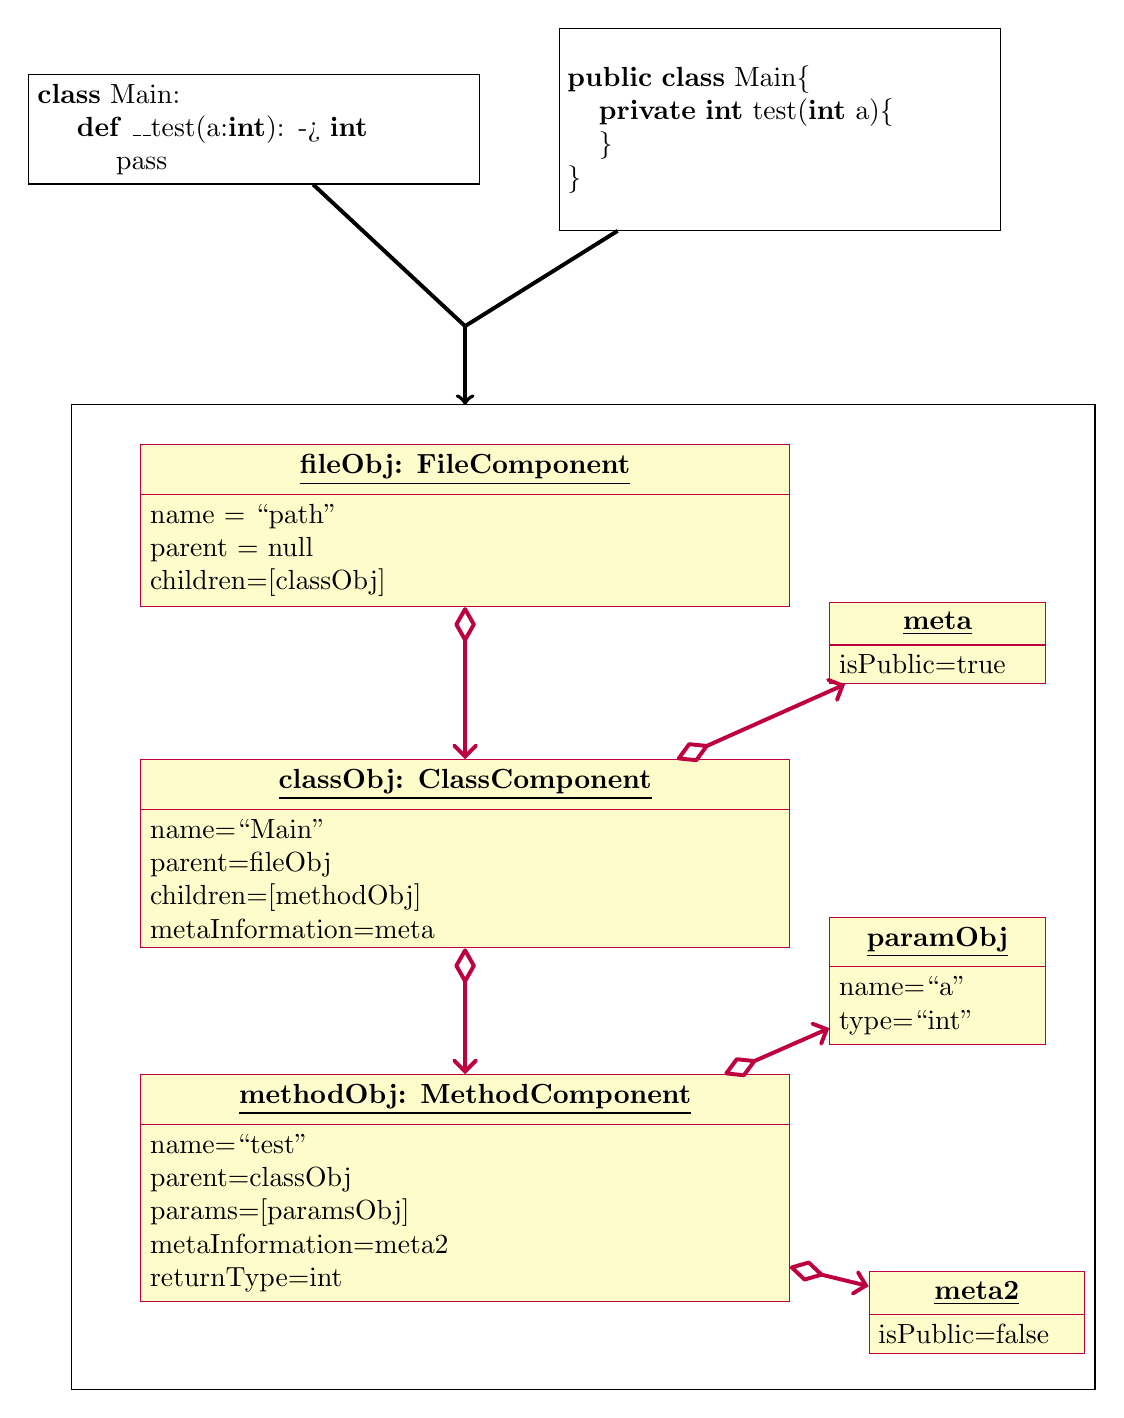
\begin{tikzpicture}
 \pgfmathsetlengthmacro\breite{6cm}
\pgfmathsetlengthmacro\hoehe{2.567cm}
\pgfmathsetlengthmacro\InnerSep{0.4cm}
\node[draw,
anchor=center, 
inner sep=0pt, 
minimum width=5cm, text width=6cm-\InnerSep,
align=justify,
minimum height=\hoehe
] (java) {
  \hspace*{0.1cm}\textbf{public} \textbf{class} Main\{\newline 
     \hspace*{0.5cm}\textbf{private} \textbf{int} test(\textbf{int} a)\{\newline
    \hspace*{0.5cm}\}\newline
\hspace*{0.1cm}\}

};
\node[draw,text width=5.5cm, left = of java](python){
\textbf{class} Main:\newline
     \hspace*{0.5cm}\textbf{def} \_\_test(a:\textbf{int}): -> \textbf{int}\newline
         \hspace*{1cm}pass

};
\draw[line width=0.05cm] (python) -- (-4,-2.5) ;
\draw [line width=0.05cm](java) -- (-4,-2.5);
\draw[->,thick,line width=0.05cm] (-4,-2.5) -- (-4,-3.5);
\draw [] (-9,-3.5) rectangle(4,-16);
\begin{scope} {0,-10}
       \begin{object}[text width=8cm]{fileObj}{-4,-4}
        \instanceOf{FileComponent}
        \attribute{name = \enquote{path}}
        \attribute{parent = null}
        \attribute{children={[}classObj{]}}
      \end{object}
      \begin{object}[text width=8cm]{classObj}{-4,-8 }
        \instanceOf{ClassComponent}
        \attribute{name=\enquote{Main}}
        \attribute{parent=fileObj}
        \attribute{children={[}methodObj{]}}
          \attribute{metaInformation=meta}
      \end{object}
    \begin{object}[text width=8cm]{methodObj}{-4,-12}
        \instanceOf{MethodComponent}
        \attribute{name=\enquote{test}}
        \attribute{parent=classObj}
        \attribute{params={[}paramsObj{]}}
        \attribute{metaInformation=meta2}
        \attribute{returnType=int}
      \end{object}
      \begin{object}[text width=2.5cm]{paramObj}{2,-10}
        \attribute{name=\enquote{a}}
        \attribute{type=\enquote{int}}
      \end{object}
    \begin{object}[text width=2.5cm]{meta}{2,-6}
        \attribute{isPublic=true}
      \end{object}
    \begin{object}[text width=2.5cm]{meta2}{2.5,-14.5}
        \attribute{isPublic=false}
      \end{object}
\end{scope}
\begin{scope}[line width=0.05cm]
    \aggregation{fileObj}{}{}{classObj}{}{}
     \aggregation {classObj}{}{}{methodObj}{}{}
      \aggregation {methodObj}{}{}{paramObj}{}{}
    \aggregation {classObj}{}{}{meta}{}{}
        \aggregation {methodObj}{}{}{meta2}{}{}
\end{scope}

    
\end{tikzpicture}
}
     
     \caption{Objektdiagramm aus Java- und Python-Code}
     \label{fig:python_java_comp}
 \end{figure}

Abbildung \ref{fig:python_java_comp} veranschaulicht, wie eine einfache Datei in die Objektstruktur umgewandelt werden kann. Dabei werden eine einfache Java-Datei und eine semantisch äquivalente Python-Datei als Beispiel verwendet, um zu zeigen, dass aus beiden Sprachen eine gleiche Objektstruktur erzeugt werden kann. Dabei wurden zur Übersichtlichkeit einige nicht relevanten Attribute entfernt.



Das Programm in beiden Sprachen besteht aus einer öffentlichen Klasse \textit{Main} und einer privaten Methode \textit{test}, die einen Parameter \textit{a} als Ganzzahl erhält und eine Ganzzahl zurückgibt. Die höchste Hierarchieebene ist immer ein \textit{FileComponent}. Diese Datei enthält hier genau ein Kind namens \textit{classObj}, könnte aber in anderen Fällen auch mehrere Kinder (wie z.~B. Klassen enthalten). Die Klasse besitzt zudem einen Verweis auf ihren Elternteil. Außerdem enthält das \textit{classObj} eine Referenz auf Metainformationen, die hier nur angeben, dass die Klasse öffentlich ist. In diesen Metainformationen könnten auch andere relativ sprachspezifische Informationen definiert werden, falls sie für Metriken relevant sein könnten. Die Klasse enthält wiederum genau die Methode als einziges Kind. Die Methode hat ebenfalls einen Verweis auf die Metainformationen, welche die Methode als privat markieren. Außerdem hat die Methode einen \textit{returnType} und einen Verweis auf die Liste der Parameter, die wiederum aus einem Namen und einem Datentyp bestehen. Das Feld \textit{comment}, welches einen Verweis auf den strukturierten Kommentar liefert, wird in dieser Abbildung nicht dargestellt, da es bei den Dateien keine Dokumentation gibt und es somit den Wert \textit{null} hat.

Die Beziehungen der Klassen, die für das Parsing zuständig sind, werden zusätzlich in Abbildung \ref{fig:uml_parsing} im Anhang \ref{appendix_parsing_uml}. als UML-Diagramm illustriert.

\subsubsection{Repräsentation der strukturierten Kommentare}\label{chapter:structured_comments}
Neben der hierarchischen Repräsentation der einzelnen Komponenten müssen auch die strukturierten Kommentare (wie z.~B. Javadoc) geeignet in eine Datenstruktur umgewandelt werden. Wie in Kapitel \ref{chapter:javadoc}
 erläutert, besteht ein strukturierter Kommentar in vielen Fällen aus zwei Teilen. Der erste Teil ist eine allgemeine Beschreibung der Komponente. Im zweiten Teil werden bestimmte Strukturen genauer erläutert. So können einzelne Parameter erklärt werden oder der Rückgabewert beschrieben werden. 
 Dieser Aufbau findet sich auch in \textit{Doxygen} \cite{doxygen} oder \textit{Docstring} \cite{docstring}, sodass diese Struktur als Grundlage genommen wird. 
 
 Ein strukturierter Kommentar besteht also aus einer generellen Beschreibung, die auch weggelassen werden kann. Anschließend folgen null bis beliebig viele Tags. Jeder Tag besteht aus einem Typ (z.~B. \enquote{@param}, \enquote{@return} oder \enquote{@throws}), einem optionalen Parameter, welcher von einigen Tags benötigt wird und der Beschreibung des Tags. Die Namen der Tags sind generalisiert, dies bedeutet, dass unabhängig von der Programmiersprache der Tag zur Beschreibung eines Parameters immer \enquote{@param} heißen muss. Dies muss bei der Entwicklung eines Parsers beachtet werden. 
 
 Ein strukturierter Kommentar kann ebenfalls spezielle Elemente (wie z.~B. \ac{HTML}-Elemente oder Inline-Tags) enthalten. Hier werden diese Elemente unverarbeitet gelassen, also unverändert mit dem Rest des Kommentars als Zeichenkette gespeichert. Metriken, die diese Informationen benötigen, müssen diese Elemente also selbstständig extrahieren. Andere Metriken (wie z.~B. die Metriken in Kapitel \ref{chapter:metrics_semantic}) benötigen diese speziellen Elemente nicht, sodass eine einheitliche Schnittstelle, die sowohl die natürliche Sprache als auch die speziellen Elemente berücksichtigt und  zudem relativ programmiersprachenunabhängig sein müsste, viele Herausforderungen mit sich bringt.   
 
 Wird kein strukturierter Kommentar angegeben, so liefert der entsprechende Getter \textit{getComment} den Wert \enquote{null} zurück. 
\section{Konzeption der Metriken}\label{chapter:metric_conception}
Nachdem eine Datei in ihre einzelnen Komponenten zerlegt wurde, kann die Qualität der Softwaredokumentation überprüft werden. Jede gefundene Komponente besitzt einen Verweis auf die dazugehörige Dokumentation, die bei Nichtvorhandensein auch null sein kann. Anhand dieser Referenz kann geprüft werden, ob die Softwaredokumentation der Komponente ausreichend ist. Zur Bewertung der Dokumentation gibt es verschiedene  Möglichkeiten. Beispielsweise könnte überprüft werden, ob eine Komponente dokumentiert oder undokumentiert ist. Eine weitere Möglichkeit wäre es, die Verständlichkeit der Dokumentation zu prüfen. Alle diese Vorgehensweisen basieren auf Metriken, die auf wissenschaftliche Studien beruhen oder zumindest plausibel sind. In diesem Abschnitt wird ein Konzept erläutert, um eine Metrik zu implementieren. Anschließend wird beschrieben, wie die Ergebnisse jeder Metrik zusammengefasst werden, um ein Endresultat zu erhalten. 

\subsection{Implementation einer Metrik}\label{chapter:metric_impl}
Damit eine Metrik die Dokumentation bewerten kann, benötigt sie Zugriff auf die Komponente. Außerdem muss sie ihr Ergebnis irgendwie veröffentlichen bzw. zwischenspeichern, damit es später weiterverarbeitet werden kann. Des Weiteren ist nicht jede Metrik mit jeder Komponente kompatibel. Eine Metrik, die überprüft, ob jeder Methodenparameter dokumentiert ist, kann diese Aufgabe bei anderen Komponentenarten nicht erfüllen. Zudem sollte es die Möglichkeit geben, das Verhalten einer Metrik mittels Parameter anzupassen, damit die Metrik konfigurierbar bleibt. Außerdem sollte eine Metrik bei der Bewertung auch begründen, warum die Dokumentation einer Komponente nicht ausreichend ist. Zuletzt soll der Benutzer des Tools selbst auswählen können, welche Metriken angewendet werden sollen, da nicht jede Metrik immer sinnvoll ist. 

Eine Möglichkeit, diese Anforderung für eine Metrik umzusetzen, ist die Verwendung einer Methode pro Metrik, welche die Komponente und die Parameter als Eingabe erhält und daraus die Bewertung und eventuelle Begründung ermittelt und zurückgibt. Allerdings ist dieser Ansatz sehr prozedural, denn es gibt beispielsweise keine Kapselung zwischen den Metriken.  

Ein anderer Ansatz, der hier auch gewählt wird, ist es, jede gewünschte Metrik als Klasse zu implementieren. Jede implementierte Metrik kann somit die notwendigen Berechnungen abgekapselt von anderen Metriken erledigen, was die Wartbarkeit verbessert. Um trotzdem für eine einheitliche Schnittstelle zu sorgen, muss jede zu implementierende Metrik von einer abstrakten Basisklasse \textit{(DocumentationAnalysisMetric)} erben. Wenn eine neue Metrik implementiert werden soll, muss eine neue Klasse erstellt werden, die von dieser abstrakten Basisklasse erbt. Eine Instanz dieser Klasse wird im Folgenden \textbf{Metrikobjekt} genannt und repräsentiert eine konkrete Implementierung der Metrik, die bei der Bewertung der Dokumentation berücksichtigt werden kann. Um diese Bewertung durchzuführen, muss geprüft werden, ob eine Metrik mit einer Komponente kompatibel ist. Dies wird durch die  Methode \textit{shallConsider} erledigt,  welche dementsprechend einen Wahrheitswert zurückgibt. Die anschließende Analyse erfolgt durch die Methode \textit{analyze}. Diese führt den metrikspezifischen Algorithmus aus und speichert das Ergebnis wie in Kapitel \ref{chapter:store_metric} beschrieben, damit es zu einem Gesamtergebnis verarbeitet werden kann.

Da eine Metrik auch parametrisierbar sein soll, müssen bei der Instanziierung  eines Metrikobjektes Parameter übergeben werden, die von der Implementation der Metrik zur Modifikation des Verhaltens der Metrik verwendet werden können. Diese Parameter werden sehr abhängig von der Metrik sein, sodass eine einheitliche Schnittstelle nur schwer umsetzbar ist. Daher werden die Parameter als Datentyp \textit{any} übergeben, sodass es keine Typüberprüfung gibt. Alternativ wäre eine assoziative Liste möglich, bei dem ein Parametername als Zeichenkette ein Wert zugeordnet wird, aber auch hier könnte keine Überprüfung eines Datentypes vorgenommen werden. 

Eine  weitere Voraussetzung für ein Metrikobjekt ist ein eindeutiger Name. Dadurch kann die gleiche Metrik mit unterschiedlichen Parametern verwendet werden. Außerdem wird so eine Zuordnung von Gewichten vereinfacht. Standardmäßig besteht dieser eindeutige Name aus dem Namen der implementierten Metrik, gefolgt von einem Unterstrich und einer fortlaufenden Nummer. 

Ein UML-Diagramm der relevanten Klassen, die für die Berechnung der Dokumentationsqualität zuständig sind, befindet sich in Abbildung \ref{fig:uml_metrics} im Anhang \ref{appendix_metrics_uml}.


\subsubsection{Bewertung der Dokumentation}
Die Methode \textit{analyze} muss eine Bewertung darüber abgeben, ob die Qualität der Dokumentation ausreichend ist. Für die Repräsentation dieser Bewertung gibt es viele Möglichkeiten, allerdings ist eine numerische Bewertung mittels einer Intervallskala am sinnvollsten, da so der arithmetische Mittelwert, der Median etc. berechnet werden kann, was für die Bildung des Gesamtergebnisses wichtig ist.
Die numerische Bewertung soll eine Aussage über die Dokumentationsqualität liefern. Eine Bewertung von 0 steht für eine sehr schlechte bis nicht existente Dokumentation und die Bewertung 100 steht für eine exzellente Dokumentation, sodass die Bewertung sich als Prozent lesen lassen kann. Das Ergebnis einer implementierten Metrik sollte diesen Wertebereich nicht verlassen, da eine Fehlerbehandlung nicht implementiert ist. Bei Metriken, die per Design schon einen prozentualen Wert zurückgeben, wird diese Vorgabe stets eingehalten. Bei anderen Metriken (z.~B. die Flesch-Metrik in Kapitel \ref{chapter:metrics_semantic}) sollte eine mathematische Funktion gefunden werden, die das Ergebnis der Metrik auf den Wertebereich 0 bis 100 abbildet. Die genaue Umsetzung hängt von der Metrik ab. In jedem Falle sollte es für eine Metrik Ergebnisse geben, die auf eine gute bzw. schlechte Dokumentation hindeuten, damit diese auf 100 bzw. 0 abgebildet werden können. Nur durch diese Einschränkung auf einen fixen Wertebereich ist es möglich, den Mittelwert, Median etc. zu bilden und so eine Vergleichbarkeit zu ermöglichen. 

\subsubsection{Verwaltung der Metriken}

Für die spätere Ausführung der Metriken ist es sinnvoll, eine zentrale Stelle zu haben, welche die Verwaltung der Metriken übernimmt. Diese zentrale Stelle entkoppelt die Verwaltung der Metriken von dem restlichen Programmcode und sorgt so für eine bessere Struktur des Programms. Diese zentrale Komponente ist der \textbf{Metrikmanager}. Der Metrikmanager ist eine statische Klasse, die von allen Modulen des Tools benutzt werden kann, welche mit den Metriken arbeiten müssen.  

Eine wichtige Funktion des Metrikmanagers ist das Erzeugen neuer Metriken. Zwar wäre es möglich, die Metriken direkt zu instanziieren, wenn sie benötigt werden, allerdings entsteht dadurch eine direkte Abhängigkeit zwischen der Metrik und dem Modul, welches eine Metrik erzeugen möchte. Zur Vermeidung dieser direkten Abhängigkeit können Fabrikmethoden verwendet werden, bei dem ein Objekt nicht direkt erzeugt wird, sondern mittels einer Abfrage durch eine bestimmte Methode erzeugt wird und anschließend an das anfragende Objekt zurückgegeben wird \cite[S.~149--161]{gamma2015design}.

Basierend auf dieser Idee kann ein Modul, das ein konkretes Metrikobjekt benötigt, den Metrikmanager mit der Instanziierung beauftragen. Dabei benötigt der Metrikmanager eine Zeichenkette, um eine konkrete abgeleitete Klasse zu identifizieren, von der das neue Metrikobjekt instanziiert werden soll. Diese Zeichenkette wird eindeutig einer bestimmten abgeleiteten Klasse zugeordnet, sodass bei der Implementation einer neuen Metrik ein neuer Name spezifiziert werden muss. Alle Zeichenketten, die für eine bestimmte Metrik stehen, werden in einer Konstantensammlung  (\textit{Enum}) definiert, die ebenfalls bei der Definition einer neuen Metrik ergänzt werden muss.  Das neue Metrikobjekt benötigt, wie in Kapitel \ref{chapter:metric_impl} beschrieben, zudem einen eindeutigen Namen und Parameter, damit es eindeutig auffindbar ist und korrekt arbeiten kann. Dieses neue Metrikobjekt wird zudem vom Metrikmanager registriert und in einer Liste gespeichert, damit es später möglich sein wird, über alle erzeugten Metriken zu iterieren. 

Der Metrikmanager bietet zudem eine Methode an, mit denen der Standardwerte für die Parameter einer Metrik abgerufen werden können, sodass diese an einer Stelle verwaltet werden können. Außerdem kann der Metrikmanager auch einen \textit{MetricResultBuilder} erzeugen, um Teilergebnisse zu einem Gesamtresultat zu aggregieren. Dies geschieht ebenfalls über eine Fabrikmethode, sodass auch hier eine Entkopplung stattfindet. 

\subsubsection{Sprachspezifische Informationen für Metriken}\label{chapter:langSpec}
Da das Tool für möglichst viele objektorientierte Programmiersprachen konzipiert werden soll, muss eine Generalisierung erfolgen, da jede Sprache ihre Eigenheiten hat und möglicherweise besondere Funktionen anbietet, die nur schwer in einem abstrakten Format zu bringen sind.

Nichtsdestotrotz können solche sprachspezifischen Eigenheiten auch in der Dokumentation erwähnt werden. Daher ist es eine sinnvolle Idee, dass Metriken auch diese Besonderheiten benutzen, um ein genaueres Bild der Dokumentationsqualität zu erfahren, ohne jedoch zu wissen, welche Programmiersprache gerade analysiert wird. Beispielsweise können die Checked-Ausnahmen in Java mit den Informationen in der Javadoc verglichen werden. Auch können hierdurch überschriebene Methoden ignoriert werden, da diese oft nicht mehr dokumentiert werden müssen.

Um solche sprachspezifischen Analysen zu erlauben, besitzt jede Metrik Zugriff auf ein Objekt der Klasse \textit{LanguageSpecificHelper}. Wenn eine neue Programmiersprache hinzugefügt werden soll, kann von dieser geerbt werden. In der Klasse \textit{LanguageSpecificHelper} sind bereits einige Methoden definiert, die einigen Metriken bei der Bewertung helfen. So bewertet die Methode \textit{rateDocumentationCompatibility}, ob die Dokumentation alle sprachspezifischen Informationen erläutert (z.~B. \enquote{@throws}). Die Methode \textit{shallConsider} kann genutzt werden, um überschriebene Methoden zu ignorieren. 

Um eine eigene Methoden hinzuzufügen, muss diese in der Basisklasse definiert werden. Diese Methode sollte in der Basisklasse keine Aktionen durchführen, sondern entweder gar nichts tun oder Rückgabewerte haben, die keinen Einfluss auf Metriken haben. Anschließend kann diese Methode in einer sprachspezifischen abgeleiteten Klasse der Basisklasse korrekt implementiert werden. Die entsprechende Methode kann dann durch Änderung des Quellcodes der Metrik an den passenden Stellen von der Metrik verwendet werden. So kann beispielsweise das Resultat einer Metrik modifiziert werden oder weitere Ergebnisse mittels des \textit{MetricResultBuilders} angefügt werden.

\subsection{Einzelergebnisse verarbeiten}\label{chapter:store_metric}

Das berechnete Ergebnis einer Komponente muss nun gespeichert werden, damit es später ausgewertet werden kann. Dazu wird ein \textit{MetricResult}-Objekt erstellt, welches das im vorherigen Unterabschnitt berechnete Ergebnis enthält. Außerdem werden hier eventuelle Begründungen und Hinweise gespeichert, die den Anwender dabei unterstützen, die Qualität der Dokumentation zu verbessern. Jede Begründung enthält den Dateipfad der betroffenen Datei, den Namen der bemängelten Komponente und ein Zeilennummerintervall, sodass der Benutzer die problematische Stelle schnell finden kann. Zuletzt werden noch Informationen gespeichert, die beschreiben, in welchem Kontext das Ergebnis produziert wurde. Dies ist für die Gewichtung der Einzelergebnisse notwendig und wird in den nächsten Unterabschnitten noch genauer erläutert. 

Für die Speicherung des Objektes gibt es zwei Möglichkeiten. Die erste Möglichkeit wäre es, dass die \textit{analyze}-Methode das \textit{MetricResult}-Objekt zurückgibt, sodass der Aufrufer damit arbeiten kann. Bei der zweiten Möglichkeit wird das Ergebnis einem anderen Objekt übergeben, der dann die Weiterverarbeitung vornimmt. Dies hat den Vorteil, dass eine Metrik kein Ergebnis zurückliefern muss, wenn es kein sinnvolles Ergebnis berechnen kann. Bei einem Rückgabewert müsste ansonsten ein ungültiger Wert wie z.~B. \textit{null} vereinbart werden. Außerdem kann eine Metrik auch mehrere Resultate speichern, was bei komplexeren Komponenten in Betracht gezogen werden könnte. Dieses weitere Objekt ist ein  \textit{MetricResultBuilder}, der wie im nächsten Unterabschnitt beschrieben, die Softwaredokumentationsqualität jeder Komponente sammelt und daraus ein Gesamtergebnis berechnet.  

\subsubsection{Einzelergebnisse aggregieren}
Da ein Softwareprojekt aus Tausenden von Dateien bestehen kann, die wiederum aus verschiedenen Komponenten bestehen, müssen die Einzelergebnisse aggregiert werden, um so am Ende ein Gesamtergebnis zu erhalten, das zur Einschätzung der Qualität der Softwaredokumentation genutzt werden kann. Dazu wird dem \textit{MetricResultBuilder} jedes Ergebnis mittels der \textit{processResult}-Methode mitgeteilt, welches das Ergebnis in einer Liste speichert. Wenn alle Metriken verarbeitet sind, wird daraus ein Gesamtresultat gebildet. Dies geschieht durch die Methode \textit{getAggregratedResult}. Dabei wird standardmäßig ein arithmetischer Mittelwert gebildet.

Neue Algorithmen (wie z.~B. der Median oder der gewichtete Mittelwert) können implementiert werden, indem von dieser Klasse abgeleitet wird und die \textit{getAggregratedResult}-Methode überschrieben wird. 

Ein \textit{ResultBuilder} basiert auf dem Vorbild des Design-Patterns \enquote{Builder} aus \cite[S. 139--149]{gamma2015design}, da dieser aus einzelnen Metrikresultaten ein vollständiges Metrikergebnis baut.


 
\subsubsection{Zuordnung der Gewichte}\label{chapter_weights_assign}
Für einige Algorithmen muss eine Gewichtung vorgenommen werden, um bestimmte Ergebnisse besser oder schlechter zu bewerten. Dazu muss jedes Teilergebnis ein Gewicht zugeordnet werden. 

Insgesamt kann ein Teilergebnis anhand von drei Kategorien gewichtet werden. Durch die Gewichtung aufgrund der verwendeten Metrik können bestimmten Metriken einen größeren Einfluss auf das Gesamtergebnis haben, wenn diese als vertrauenswürdiger empfunden werden. Durch die Gewichtung von Dateien kann beispielsweise die öffentliche Schnittstelle einen größeren Einfluss auf die Bewertung nehmen, da diese Komponenten bzw. Dateien sehr kritisch sein können und daher gut verstanden werden müssen. Auch eine Gewichtung nach Komponenten kann in bestimmten Situationen sinnvoll sein. So kann beispielsweise argumentiert werden, dass Methoden, die durch ihre Parameter, Rückgabewerte und geworfenen Ausnahmen komplexer als Felder sind, höher gewichtet werden sollen.

Die Zuordnung der Gewichte erfolgt über einen \textit{WeightResolver}, welches eine Schnittstelle anbietet, um einen Bezeichner auf ein Gewicht abzubilden. Bei dem eindeutigen Namen eines Metrikobjektes kann hierfür eine assoziative Liste verwendet werden. Auch bei Komponenten, die durch ihren Klassennamen (wie z.~B. \textit{ClassComponent}) repräsentiert werden, ist  eine solche assoziative Liste sinnvoll, da nur eine begrenzte Anzahl an Metriken bzw. Komponenten existieren kann.
Für Dateipfade ist dies allerdings nicht praktikabel, da es eine Vielzahl an Dateien geben kann. Stattdessen können hier ähnlich wie bei der Filterung von Dateien in Kapitel \ref{chapter:traversing} Wildcard-Patterns verwendet werden. Eine assoziative Liste kann dazu jedes Wildcard-Patterns und das dazugehörige Gewicht speichern. Bei einer Abfrage kann das Gewicht des ersten Eintrages zurückgegeben werden, bei dem der Dateipfad mit dem Wildcard-Pattern kompatibel ist. Dies ermöglicht es, ganze Verzeichnisse oder Dateien mit bestimmten Namen stärker zu gewichten. 

Bei der Suche nach dem passenden Gewicht zu den Dateien und Komponenten kann es vorkommen, dass das passende Gewicht nicht gefunden wird. Um hierdurch entstehende Probleme zu vermeiden, wird ein Standardwert genommen (z.~B. 1). 

Jedes \textit{MetricResult}-Objekt enthält ein Tupel von drei Namen, welche die Quelle dieses Ergebnisses repräsentieren (Dateipfad, Komponententyp und eindeutiger Metrikname). Der Dateipfad beschreibt, in welcher Datei die Komponente liegt, die durch dieses Teilergebnis analysiert wurde. Der Komponententyp enthält den Klassennamen der Komponente und gibt somit Aufschluss darüber, ob diese Komponente eine Klasse, Methode etc. ist. Bei einer Klasse würde beispielsweise die Zeichenkette \enquote{ClassComponent} gespeichert werden. Durch den eindeutigen Metrikname (siehe Kapitel \ref{chapter:metric_impl}) wird  festgelegt, welche Metrik dieses Teilresultat produzierte. Alternativ könnte auch hier der Klassenname der Metrik verwendet werden. Allerdings kann eine Metrik durch Verwendung verschiedener Parameter auch mehrfach angewendet werden, sodass eine unterschiedliche Gewichtung möglich wäre. Daher ist der eindeutige Name hier sinnvoller.

  \begin{figure}[h!]
  \centering
 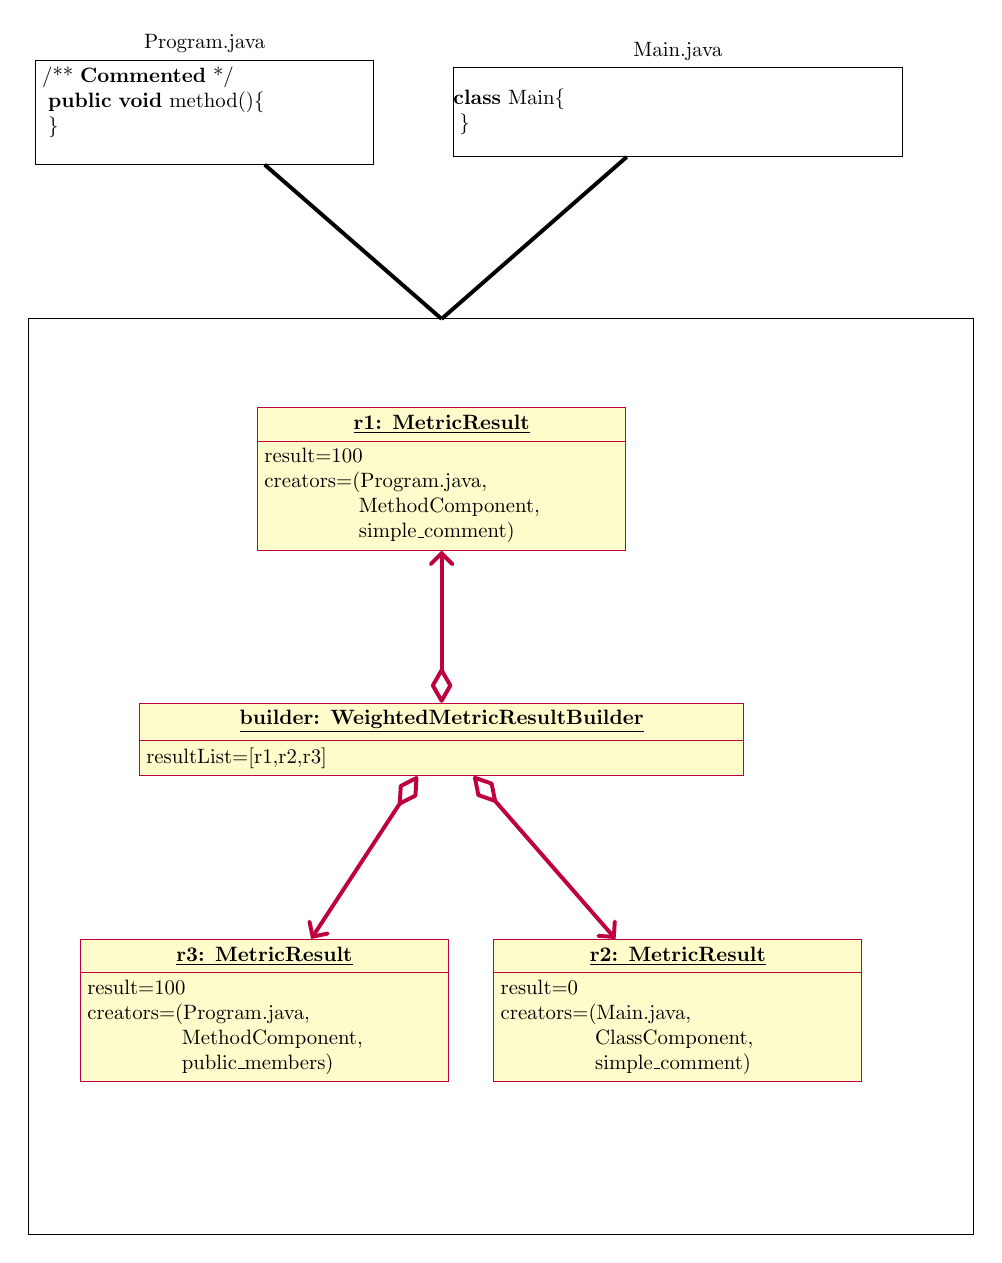
\begin{tikzpicture}[scale=0.75, every node/.style={scale=0.75}]
 \pgfmathsetlengthmacro\breite{6cm}
\pgfmathsetlengthmacro\hoehe{2.567cm}
\pgfmathsetlengthmacro\InnerSep{0.4cm}
\node[draw,
anchor=center, 
inner sep=0pt, 
minimum width=5cm, text width=8cm-\InnerSep,
align=justify,minimum height=1.5cm] (java) {\textbf{class} Main\{\newline 
\hspace*{0.1cm}\}};

\node[draw,text width=5.5cm, left = of java](java2){
/** \textbf{Commented} */ \newline
     \hspace*{0.1cm}\textbf{public} \textbf{void} method()\{\newline
    \hspace*{0.1cm}\}\newline
};
\draw[line width=0.05cm]    (java2) -- (-4,-3.5) ;
\draw [line width=0.05cm](java) -- (-4,-3.5);
\draw[thick,line width=0.05cm] (-4,-3.5) -- (-4,-3.5);

\node[above=-0.0 of java2,line width=0cm]{Program.java};

\node[above=-0.0 of java,line width=0cm]{Main.java};


\draw [] (-11,-3.5) rectangle(5,-19);
\begin{scope} {0,-10}
       \begin{object}[text width=10cm]{builder}{-4,-10}
        \instanceOf{WeightedMetricResultBuilder}
        \attribute{resultList={[r1,r2,r3]}}
      \end{object}
      \begin{object}[text width=6cm]{r1}{-4,-5 }
        \instanceOf{MetricResult}
        \attribute{result=100}
        \attribute{creators=(Program.java,\newline
        \hspace*{1.6cm}MethodComponent, \newline
        \hspace*{1.6cm}simple\_comment)}
      \end{object}
      
        \begin{object}[text width=6cm]{r2}{0,-14 }
        \instanceOf{MetricResult}
        \attribute{result=0}
        \attribute{creators=(Main.java,\newline
        \hspace*{1.6cm}ClassComponent,\newline
        \hspace*{1.6cm}simple\_comment)}
      \end{object}
      
           \begin{object}[text width=6cm]{r3}{-7,-14 }
        \instanceOf{MetricResult}
        \attribute{result=100}
        \attribute{creators=(Program.java,\newline
       \hspace*{1.6cm}MethodComponent,\newline
       \hspace*{1.6cm}public\_members)}
      \end{object}
      

   
\end{scope}
\begin{scope}[line width=0.05cm]
    \aggregation{builder}{}{}{r1}{}{}
    \aggregation{builder}{}{}{r2}{}{}
    \aggregation{builder}{}{}{r3}{}{}

\end{scope}

    
\end{tikzpicture}
     
     \caption{ Veranschaulichung der Bildung eines Gesamtergebnisses}
     \label{fig:metric_weighting}
 \end{figure}
Durch dieses Tupel kann für jedes Teilergebnis die Gewichtung der Metrik, der Komponente und des Dateipfades  abgerufen werden. Durch Multiplikation  aller Gewichtungen entsteht ein Gesamtgewicht.

Abbildung \ref{fig:metric_weighting} veranschaulicht anhand eines vereinfachten Objektdiagramms die Bildung eines Gesamtresultats mittels Gewichtung von verschiedenen Ergebnissen, indem der gewichtete Mittelwert aus Kapitel \ref{chapter:weighted_aggreg} verwendet wird. Hier wird ein hypothetisches Projekt mit zwei Dateien analysiert. Die erste Datei \enquote{Program.java} enthält nur eine öffentliche Methode \textit{method}, was in Java eigentlich nicht möglich ist, aber hier zur Vereinfachung zugelassen sein soll. Die zweite Datei \enquote{Main.java} enthält eine nichtöffentliche Klasse \textit{Main}. In diesem Beispiel werden zwei Metriken verwendet. Die erste Metrik prüft das Vorhandensein der Dokumentation bei allen Komponenten, während die zweite Metrik nur öffentliche Komponenten betrachtet (siehe Kapitel \ref{chapter:metrics_coverage}). In diesem Beispiel soll die Datei \enquote{Main.java} mit dem Faktor $3$ gewichtet werden. Methoden sollen mit dem Faktor $4$ gewichtet werden. Die zweite Metrik \textit{public\_members} wird mit dem Faktor $2$ gewichtet. Alle anderen Dateien, Komponenten und Metriken werden mit dem Standardfaktor $1$ gewichtet.

Das erste Teilergebnis \textit{r1} ist 100, da es die  Methode \textit{method} beschreibt, welche dokumentiert ist. Auch das dritte Teilergebnis \textit{r3} hat den Wert 100, da es die gleiche Komponente nur mit der zweiten Metrik beschreibt. Das zweite Teilergebnis \textit{r2} hat den Wert 0, da es die undokumentierte Klasse \textit{Main} beschreibt.  Es gibt kein weiteres Teilergebnis von \enquote{Main.java}, da die zweite Metrik jegliche nichtöffentliche Komponenten ignoriert. Die Teilergebnisse werden durch den \textit{WeightedMetricResultBuilder} intern gespeichert. 

Das Teilergebnis jeder gefundenen Komponente enthält gemäß dem obigen Vorgehen ein Tupel aus Dateiname, Komponentenname und Metrikname. Beispielsweise enthält das erste  Teilergebnis \textit{r1} das Tupel \enquote{(Program.java, MethodComponent, simple\_comment)}, wobei die einzelnen Bestandteile des Tupels Zeichenketten sind. Basierend auf diesen Informationen kann der \textit{WeightedResultBuilder} eine Gewichtung vornehmen. Das erste Teilergebnis würde mit dem Faktor $1*4*1=4$ gewichtet werden, da es von einer Methode stammt  und ansonsten nicht besonders gewichtet wird. Das zweite Teilergebnis erhält das Gewicht $3*1*1=3$, da es von der Datei \enquote{Main.java} stammt. Zuletzt besitzt das dritte Teilresultat die Gewichtung $1*4*2=2$, da es von der zweiten Metrik berechnet wurde und auch von einer Methode stammt. 

Basierend auf diesen Teilresultaten kann ein Gesamtergebnis berechnet werden. Hierzu wird jedes Ergebnis mit dessen Gewicht multipliziert und anschließend wird durch die Summe der Gewichte geteilt. Bezogen auf das Beispiel würde die Rechnung folgendermaßen aussehen:
\begin{equation}
    \frac{4*100 + 3*0 + 8*100}{4+3+8}=80
\end{equation}
Dieses Ergebnis ist dann Maß für die Bewertung der Dokumentationsqualität dieses hypothetischen Projektes. 









\begin{comment}
\begingroup
\renewcommand{\cleardoublepage}{} % TODO maybe removing this and next
\renewcommand{\clearpage}{}
\chapter{Umsetzung}\label{chapter:program}
\endgroup
In diesem Kapitel wird auf die Umsetzung der in Kapitel \ref{chapter_conception} beschriebenen Architektur eingegangen. In Kapitel \ref{chapter:tool_running} wird zunächst erläutert, wie das Programm konkret ausgeführt wird, um die Dokumentationsqualität zu ermitteln. Danach wird in Kapitel \ref{chapter:traversing} beschrieben, wie das Programm die einzelnen Java-Dateien findet, damit diese weiterverarbeitet werden können.  Außerdem wird in Kapitel \ref{chapter:antlr4_impl} erläutert, wie ANTLR4 verwendet wird, um Java-Dateien zu parsen. Daraufhin wird erklärt, wie die strukturierten Kommentare geparst werden (Kapitel \ref{chapter:comment_parsing}).  In Kapitel \ref{chapter:conf} wird die Konfiguration des Tools erläutert. Um auch einen Vergleich zwischen den aktuellen und den vorherigen Zustand der Dokumentationsqualität zu ermöglichen, wird in Kapitel \ref{chapter:saving} beschrieben, wie das letzte Ergebnis der Bewertung gespeichert werden kann. In Kapitel \ref{chapter:github_actions_impl} wird erklärt, wie das Programm in GitHub Actions eingebunden wird und wie es so genutzt werden kann. Zum Abschluss werden in Kapitel \ref{chapter:metrics} und \ref{chapter:algos_aggregation} die implementierten Metriken und die implementierten Aggregationsalgorithmen erläutert. 


\hfill
\section{Ausführung des Programms}\label{chapter:tool_running}
In diesem Unterabschnitt wird beschrieben, wie das Programm die in Kapitel \ref{chapter_conception}
beschriebenen Arbeitspakete nutzt, um die Qualität der Softwaredokumentation zu bewerten. 

Die Koordination des Programms wird in der Datei \enquote{index.ts} durchgeführt, die als Einstiegspunkt des Programms verstanden werden kann. In dieser Datei werden die einzelnen Module des Programms in der richtigen Reihenfolge aufgerufen und die Ergebnisse eines Moduls werden durch die \enquote{index.ts}-Datei an das folgende Modul/Arbeitspaket übergeben, soweit sie dort benötigt werden. Dadurch sind die Module voneinander entkoppelt und greifen nicht direkt aufeinander zu. 

Im ersten Schritt  muss die Konfiguration des Programms geladen werden. Dazu wird das Arbeitsverzeichnis von der Kommandozeile gelesen. Basierend auf das Arbeitsverzeichnis kann dann die Konfiguration des Tools geladen werden, wie es in Kapitel \ref{chapter:conf} beschrieben ist.  

Anschließend müssen einige Objekte  initialisiert werden. Hierzu werden die Werte aus der Konfiguration (z.~B. der Konfigurationsdatei) verwendet. Beispielsweise kann durch \textit{builder} der Algorithmus festgelegt werden, der die Einzelergebnisse der einzelnen Metriken zu einem Gesamtresultat kombiniert. Dazu wird eine Fabrikmethode verwendet, da damit die Konstruktion eines Objektes aus einer Zeichenkette möglich ist und somit der Anwender in der Konfiguration nur eine bestimmte Zeichenkette oder ID zur Konstruktion eines komplexeren Objektes angeben muss \cite[S.~149--161]{gamma2015design}. Zudem werden die Metriken, die zur Analyse verwendet werden sollen, durch den Metrikmanager registriert.

Außerdem wird eine assoziative Liste für die Dateien und die Metriken erstellt, die einem eindeutigen Metriknamen bzw. einem Wildcard-Pattern einer Datei ein Gewicht zuordnet. Diese Liste kann einem \textit{WeightResolver} übergeben werden, der wiederum dem  \textit{MetricResultBuilder} übergeben wird. Falls dieser keine Gewichtung benötigt, werden diese Informationen ignoriert. 

Danach müssen die relevanten Dateien gefunden werden. Dazu werden dem Traversierer (siehe Kapitel \ref{chapter:traversing}) die Wildcard-Patterns der zu inkludierenden Dateien und der auszuschließenden Dateien übergeben. Mit der Methode \textit{getRelevantFiles} werden dann alle relevanten Dateien zurückgegeben.

In nächsten Schritt muss jede Datei mit jeder Metrik geprüft werden und die Ergebnisse gesammelt werden. Hierzu wird eine verschachtelte For-Schleife verwendet. Dabei gibt es zwei Möglichkeiten zur Verschachtelung. Im ersten Fall könnte in der äußeren Schleife jede Datei und in der inneren jede Metrik durchlaufen werden. Alternativ könnte auch die innere und äußere Schleife vertauscht werden. Der erste Ansatz hat den Vorteil, dass jede Datei nur einmal geladen werden muss, was einen Geschwindigkeitsvorteil bringen kann, deshalb wird dieses Verfahren auch gewählt. Pro Iteration der inneren Schleife wird die aktuelle Datei von der jeweiligen Metrik analysiert und alle gefundenen Metrikresultate, die von den einzelnen Komponenten der Datei stammen, zu einem \textit{MetricResultBuilder} hinzugefügt.

Nach Abschluss der beiden Schleifen steht das Ergebnis durch Aggregation der Resultate in dem \textit{MetricResultBuilder} zur Verfügung und kann genutzt werden, um die Qualität der Dokumentation mit dem Grenzwert bzw. dem letzten Wert zu vergleichen. Wird bei diesem Vergleich festgestellt, dass die Dokumentationsqualität nicht ausreichend ist, wird eine Ausnahme geworfen und das Programm bricht ab. Wird das Programm mittels GitHub Actions ausgeführt, so kann durch diese Ausnahme ein Merge verhindert werden.

Die Abbildungen \ref{fig:passed} und \ref{fig:absolute} im Anhang \ref{chapter:pictures_tool} visualisieren die Ausgabe des Programmes bei einer ausreichenden bzw. mangelhaften Dokumentationsqualität.

\section{Traversierung aller relevanten Dateien und der Komponenten}\label{chapter:traversing}
Softwareprojekte bestehen aus Hunderten von Dateien, die nicht alle Quellcode enthalten. Beispielsweise gehören Konfigurationsdateien, Ressourcendateien wie Bilder oder binäre Dateien zu den Dateien, bei denen eine Analyse der Softwaredokumentation im Hinblick auf die begrenzte Zeit für die Bachelorarbeit nicht implementierbar ist. Daher ist es sinnvoll, bestimmte Dateien bei der Analyse auszuschließen beziehungsweise nur bestimmte Dateien zu betrachten. Bei einer Weiterentwicklung des Tools nach Abschluss der Bachelorarbeit kann das Tool auf andere Dateitypen ausgeweitet werden, um so ein besseres Gesamtbild über die Softwaredokumentation zu erhalten.

Um die relevanten Dateien zu finden, wird zunächst ein übergeordnetes Verzeichnis benötigt, was bei Softwareprojekten aber der Standard sein sollte. Dieses Verzeichnis kann dann rekursiv durchlaufen werden und somit die Liste aller darin gespeicherten Dateien abgerufen werden. Die relevanten Dateien können dann durch Überprüfung ihres Dateinamens mittels bestimmter Regeln ermittelt werden, die der Benutzer des Tools festlegen kann.

Beim DocEvaluator wird hierzu die NPM-Bibliothek \textit{Minimatch} \cite{Minimatch} verwendet, die es ermöglicht, Dateinamen mit Wildcard-Patterns zu vergleichen. Zum Beispiel könnte der Dateiname \enquote{test.txt} mit der Wildcard \enquote{test.*} verglichen werden und die Bibliothek würde eine Übereinstimmung melden.

Auch die Komponenten einer Datei müssen traversiert werden, damit bei jeder Komponente die Dokumentation überprüft werden kann. Da die Komponenten wie in Kapitel \ref{chapter:parsing} beschrieben rekursiv aufgebaut sind, kann dies mittels einer Tiefensuche durchgeführt werden.

\subsubsection{Ignorieren bestimmter Kommentare}

Unter Umständen kann es sinnvoll sein, bestimmte Komponenten bei der Bewertung auszulassen, weil sie beispielsweise noch nicht vollständig implementiert sind, in einer nicht-englischen Sprache dokumentiert sind oder ein anderer gewichtiger Grund existiert. Für diesen Fall kann die allgemeine Beschreibung der Dokumentation einer Komponente  den Begriff \enquote{\%ignore\_this\%} oder \enquote{\%ignore\_node\%} enthalten. Bei Ersterem wird nur diese Komponente ignoriert und als nicht existent betrachtet. Bei Zweiterem werden sowohl diese Komponente als auch alle Kinder dieser Komponente ignoriert, sofern sie existieren.




\section{Implementierung von ANTLR4 für Java}\label{chapter:antlr4_impl}

Für die Programmiersprache Java steht eine ANTLR4-Grammatik, die auf GitHub unter der BSD-Lizenz angeboten wird, zur Verfügung \cite{ANTLRgrammarforjava}, allerdings ignoriert diese Grammatik alle Kommentare. Daher müssen einige Änderungen sowohl am Lexer als auch am Parser vorgenommen werden. Im Lexer werden standardmäßig alle Tokens aus einem Kommentar in einem versteckten Kanal gespeichert, was dazu führt, dass diese Tokens vom Parser ignoriert werden. Um dieses Problem zu lösen, wird das Verhalten durch Definition eines neuen Tokens so geändert, dass Javadoc-Kommentare auch vom Parser verarbeitet werden können, aber mehrzeilige und einzeilige Kommentare weiterhin ignoriert werden. Einzeilige Kommentare sind hier nicht relevant, da sie kein Javadoc enthalten.

Mehrzeilige Kommentare könnten theoretisch auch berücksichtigt werden, da einige Entwickler diese anstelle von Javadoc benutzen. Allerdings werden solche mehrzeiligen Kommentare vor Komponenten nicht von Tools erkannt und haben daher einen geringeren, aber durchaus vorhandenen Nutzen \cite[S.~4]{HowDocumentationEvolvesoverTime}. Deshalb werden Komponenten, die zwar mit mehrzeiligen Kommentaren, aber nicht mit Javadoc dokumentiert sind, wie undokumentierte Komponenten betrachtet. Für einen Entwickler sollte es so schnell möglich sein, solche nicht korrekt dokumentierten Komponenten zu identifizieren und deren mehrzeilige Kommentare in gültige Javadoc-Kommentare umzuwandeln und so die Qualität der Dokumentation zu erhöhen. Für andere Programmiersprachen können jedoch normale mehrzeilige wie strukturierte Kommentare betrachtet werden, wenn dies für sinnvollerer erachtet wird.

Mehr Änderungen müssen an der entsprechenden Parser-Datei \enquote{JavaParser.g4} durchgeführt werden.  Da diese Änderungen für die eigentliche Thematik dieser Bachelorarbeit nur eine untergeordnete Rolle spielen, wird hier nicht jede Änderung genauer erklärt. Tabelle \ref{tab:parser_changes} im Anhang \ref{chapter:appendix_parser_changes} listet alle Änderungen an der Parserdatei auf. Die geänderte Parserdatei und das Original befinden sich auch im digitalen Anhang im Verzeichnis \enquote{parser\_changes}. 

Um die Informationen aus einer Java-Datei mittels ANTLR4 zu verarbeiten, kann das Visitor-Pattern verwendet werden \cite[S.~400ff.]{gamma2015design}. Mit einem Visitor kann die Baumstruktur, die ANTLR4 erstellt hat, traversiert werden, damit so nur die notwendigen Informationen herausgefiltert werden. Andere Informationen (wie z.~B. Conditional-Branches) können so ignoriert werden.  
		\begin{figure} [htbp!]
			\lstinputlisting
			[caption={Codeauschnitt aus  Methoden-Visitor},
			label={lst:visit_method_example},
			captionpos=b,language=javascript, basicstyle=\footnotesize, tabsize=2, showstringspaces=false,  numbers=left]
			{figures/chapter4/visit_method_example.js}
		\end{figure}
Listing \ref{lst:visit_method_example} zeigt einen Ausschnitt vom Visitor für Methodendeklarationen aus dem Quellcode des Tools. Hier ist die Baumstruktur leicht sichtbar. Alle Einzelbestandteile einer Methode wie z. B. Bezeichner, Rückgabetyp etc. sind Kindknoten des \textit{RuleContext} und können über die Methode \textit{getChild} abgerufen werden. So werden sowohl der Bezeichner als auch der Rückgabetyp direkt als Text abgerufen. Diese  beiden Bestandteile bestehen wiederum auch aus weiteren Kindknoten, doch eine weitergehende Betrachtung ist nicht nötig, da nur die Bezeichnung als Zeichenkette benötigt wird. Andere Bestandteile wie die Methodenparameter sind jedoch komplexer, deswegen werden sie von separaten Visitors betrachtet.

\section{Parsen der strukturierten Kommentare}\label{chapter:comment_parsing}
Um die strukturierten Kommentare in das Format nach Kapitel \ref{chapter:structured_comments} zu bringen, wird eine simple Heuristik verwendet. Es werden so viele Zeilen als allgemeine Beschreibung betrachtet, bis eine Zeile auftaucht, die mit einem Tag wie z.~B. \enquote{@param} beginnt, der den allgemeinen Teil beendet.

Anschließend werden diese Tags verarbeitet. Benötigt ein Tag einen Parameter, so wird die Zeile in drei Teilen an den Leerzeichen aufgetrennt. Dabei ist der erste Teil der Typ des Tags, der zweite Teil der Parameter und der Rest (mit allen übrigen Leerzeichen) die Beschreibung des Tags.
Bei einem Tag ohne Parameter wird die Zeile in zwei Teile getrennt, wobei hier der erste Teil der Typ des Tags und der letzte Teil die Beschreibung ist.

Diese Heuristik sollte die gängigsten Javadoc-Blöcke verarbeiten können. Alternativ könnte auch ANTLR4 Javadoc parsen. Allerdings ist dies aufgrund der Mischung von natürlicher Sprache und der relativen Flexibilität von Javadoc nicht trivial und wird daher nicht implementiert. 



\section{Konfiguration des Tools}\label{chapter:conf}
Zur Nutzung des Tools werden bestimmte Informationen benötigt, die aus verschiedenen Quellen bezogen werden. Zunächst benötigt das Tool den Pfad, der die Quelldateien enthält, die nach Kapitel \ref{chapter:traversing} traversiert werden sollen. Dieser wird als namenloser Parameter über die Kommandozeile übergeben. Er ist optional, da bei dessen Fehlen das aktuelle Arbeitsverzeichnis genommen wird. Die weiteren Informationen werden aus zwei Quellen bezogen. Wenn beide Quellen fehlen, werden Standardwerte genommen. Die erste Quelle ist eine \ac{JSON}-Datei namens \mbox{\enquote{comment\_conf.json}}, welche die notwendigen Daten für die Arbeit des Programms enthält. Listing \ref{lst:example_conf} zeigt eine beispielhafte Konfigurationsdatei im \ac{JSON}-Format.

\begin{figure}[htbp]
\lstinputlisting
[caption={Beispielhafte Konfigurationsdatei für das Tool},
label={lst:example_conf},
captionpos=b, basicstyle=\footnotesize, tabsize=2, showstringspaces=false,  numbers=left,language=JSON]
{figures/chapter4/example_conf.json}
\end{figure}

In dieser Beispieldatei  werden alle Dateien mit der Dateiendung \enquote{.java} bei der Traversierung betrachtet (Z. 1). Außerdem werden dabei keine Dateien bei der Traversierung ausgeschlossen (Z. 2). Diese beiden Werte entsprechend dabei ihre Standardwerte. Sie könnten also bei dieser Konfigurationsdatei weggelassen werden und das Programmverhalten würde sich nicht ändern.

Anschließend (Z. 4--11) werden die zu verwendenden Metriken definiert. Jede Metrik besitzt einen \textit{metric\_name}, der den Typ der Metrik spezifiziert. In Zeile 6 wäre dies beispielhaft die Metrik \enquote{Anteil der dokumentierten Komponenten an allen Komponenten} (vgl. Kapitel \ref{chapter:metrics_coverage}). Anhang  \ref{appendix_metrics} beschreibt alle implementierten Metriken mit ihren Namen. Diese Namen werden vom Metrikmanager dazu genutzt, um die passende Klasse zu finden und so ein Metrikobjekt zu erzeugen. Außerdem erhält jede Metrik durch \textit{unique\_name} einen eindeutigen Namen (hier z.~B. \enquote{m1}). Dieser kann auch weggelassen werden. Dann wird der eindeutige Name aus dem Namen der Metrik und einer fortlaufenden Nummerierung erzeugt. Zudem besitzt jede Metrik das Attribut \textit{weight}, welches zur Bestimmung der Relevanz bzw. des Gewichts der Metrik dient und von einem \textit{MetricResultBuilder} zur Bestimmung eines Gesamtergebnisses benutzt werden kann. Ein \textit{MetricResultBuilder}, der keine Gewichtung der Metriken benötigt, wird diese Information ignorieren. Das Gewicht ist ebenfalls optional. Bei dessen Fehlen wird das Gewicht \enquote{1} eingesetzt.  Durch \textit{params}  werden der Metrik die Parameter übergeben, die sie benötigt. Die genaue Anzahl und Struktur der Parameter hängen von der jeweiligen Metrik ab. Fehlen diese Parameter, so werden standardmäßige Parameter verwendet.

Fehlt der Eintrag \enquote{metrics}, so werden alle implementierten Metriken mit ihren Standardwerten genommen.

Als Nächstes (Z. 12) wird der Schwellwert festgelegt. Dieser Wert legt fest, ob das Programm beim Unterschreiten dieses Wertes mit einer Fehlermeldung abbrechen soll. In Zeile 13 wird der \textit{MetricResultBuilder} festgelegt, der bestimmt, wie die Einzelergebnisse aggregiert werden. In dem Beispiel werden alle Teilresultate mittels eines gewichteten Mittelwertes zu einem Gesamtergebnis aggregiert.  In Zeile 14 wird durch \mbox{\textit{ relative\_threshold }} festgelegt, um wie viel sich die Dokumentationsqualität verschlechtern muss, damit ebenfalls eine Fehlermeldung erscheint. Dies wird in Kapitel \ref{chapter:saving} genauer erläutert.



\bigskip
Die zweite Quelle für die Informationen sind die Eingabeparameter aus GitHub Actions. Dazu wird, wie in Kapitel \ref{chapter:github_actions_impl} beschrieben, jeder Parameter aus der \ac{JSON}-Datei auch in der \enquote{action.yml}-Datei übernommen. Bei der Ausführung des Programms stehen diese Eingabedaten über Umgebungsvariablen bereit. Jede Umgebungsvariable beginnt mit der Zeichenkette \enquote{INPUT\_}, anschließend folgt der Name des entsprechenden Parameters (wie in der \ac{JSON}-Datei), wobei der Name allerdings komplett in Großbuchstaben geschrieben ist. So steht  \enquote{absolute\_threshold} als \enquote{INPUT\_ABSOLUTE\_THRESHOLD} zur Verfügung.

Da es durchaus sein kann, dass sowohl eine Konfigurationsdatei existiert als auch die Umgebungsvariablen gesetzt sind, muss klar festgelegt werden, welcher Wert eines Parameters am Ende genommen wird. Bei dem Tool haben die von GitHub Actions erzeugten Umgebungsvariablen  Vorrang, da das Tool für die Verwendung in GitHub Actions konzipiert wurde.  Die Auflistung im Anhang \ref{enum:tool_javadoc_conf} listet alle Parameter des Tools nochmals auf und erläutert sie zusätzlich. 


\section{Speicherung des letzten Ergebnisses}\label{chapter:saving}
Neben der bereits erwähnten Möglichkeit, einen absoluten Grenzwert für die Dokumentationsqualität zu definieren, ist auch ein inkrementeller Vergleich interessant. Dabei wird das Ergebnis der Dokumentationsqualität zwischengespeichert. Bei einem neuen Start des Tools kann das alte Ergebnis mit dem neuen Ergebnis verglichen werden. Verschlechtert sich das Ergebnis über einen gewissen Schwellwert hinaus, so sollte der Entwickler ebenfalls gewarnt werden, selbst wenn die Dokumentationsqualität noch über der absoluten Grenze liegt. Schließlich kann dies ein Trend sein, der zum baldigen Unterschreiten des absoluten Grenzwertes führen kann. 

Der Ort zur Speicherung des letzten Wertes ist dabei flexibel. Standardmäßig wird der Wert in einer Datei namens \enquote{.evaluator\_last\_state.txt} gespeichert. Falls das Programm im Kontext von GitHub Actions ausgeführt wird, sollte allerdings beachtet werden, dass diese Datei nach der Beendigung des Workflows gelöscht wird. Dieses Problem kann dadurch gelöst werden, dass die geänderte Datei im Repository des zu analysierenden Projektes hochgeladen wird. Dies kann beispielsweise mit dem Tool \textit{Add \& Commit} \cite{add_commit} erledigt werden. Nachteilhaft ist an diesem Vorgehen allerdings, dass hierdurch in dem Commit-Verlauf automatisierte Commits erscheinen, sodass der Überblick verloren gehen kann.  Eine weitere Möglichkeit zur Speicherung des Wertes wäre es, den Wert an einen externen Server zu senden und bei einem erneuten Start diesen Wert abzurufen. 

  
\section{Einbindung in GitHub Actions}\label{chapter:github_actions_impl}
Um das Tool in GitHub Actions einzubinden, müssen einige Schritte erfolgen. Zunächst muss eine \enquote{action.yaml} geschrieben werden, die das GitHub-Repository als Aktion markiert und die notwendigen Befehle für die Ausführung enthält. Listing  \ref{lst:action} zeigt einen beispielhaften Code der Action. Zur Übersichtlichkeit wird in diesem Listing nur ein Eingabeparameter definiert. Die restlichen Eingabeparameter werden im Programm analog definiert.
\begin{figure} [htbp]
\lstinputlisting
[caption={Beispielhafte Action-Datei für das Tool},
label={lst:action},
captionpos=b, basicstyle=\footnotesize, tabsize=2, showstringspaces=false,  numbers=left,language=YAML]
{figures/chapter4/action.yml}
\end{figure}

In den ersten beiden Zeilen werden Attribute wie der Name und eine Beschreibung gesetzt. Danach (Z. 4--7) wird der Eingabeparameter für die minimal erlaubte Bewertung für die Dokumentationsqualität definiert, damit dieser von den Nutzern der Aktion verändert werden kann. In den Zeilen 8 bis 10 ist der wichtige Programmcode enthalten, in denen die Aktion als JavaScript-Aktion mit der Node-Version 16 festgelegt wird. Zudem enthält die letzte Zeile auch den Pfad zur Quellcodedatei, mit dem das Programm gestartet werden soll. 

\bigskip
Eine JavaScript-Aktion in GitHub Actions benötigt JavaScript, sodass der TypeScript-Code des Tools erst in JavaScript umgewandelt werden muss. Damit das Programm bei der Veröffentlichung einer neuen Version in einen auslieferbaren Zustand gebracht werden kann, wird ein weiterer Workflow benötigt, der bei jedem Push in dem Main-Zweig folgende Schritte ausführt:
\begin{enumerate}
    \item Klonen des Main-Branch des Repositorys (wie bei den meisten anderen Workflows)
    \item Aufruf von TSC, Konvertierung des TypeScript-Codes in JavaScript
    \item Aufruf und Benutzung von \textit{NCC} \cite{ncc}. Packen aller JavaScript-Dateien in einer einzigen Datei
    \item Kopieren der generierten Datei, die den gesamten Quellcode enthält, und der \enquote{action.yml}, in eine (neue) Branch \textit{action}. Dies wird mittels der Aktion \textit{Branch-Push} \cite{Branch-Push} durchgeführt
\end{enumerate}
Durch diese Schritte wird eine neue Branch erstellt, die nur die notwendige JavaScript-Datei und die \textit{action.yml} enthält. Dadurch können Nutzer der Aktion diese schneller herunterladen und nutzen. Es wäre auch möglich, kein \textit{NCC} zu verwenden, also alle Javascript-Dateien in die neue Branch zu kopieren, allerdings ist die hier gewählte Methode praktikabler, da dann nur ein Lesezugriff beim Starten des Programms erforderlich ist und so ein Geschwindigkeitsvorteil existiert. 

\subsubsection{Nutzung der Aktion}

Die oben erstellte Aktion kann nun von jedem GitHub-Repository verwendet werden. Dazu kann das folgende Listing \ref{lst:action_using} als zusätzlicher Schritt in einem Workflow eingebunden werden. 
\begin{figure} [htbp]
\lstinputlisting
[caption={Verwendung der Aktion in einem Workflow},
label={lst:action_using},
captionpos=b, basicstyle=\footnotesize, tabsize=2, showstringspaces=false,  numbers=left,language=YAML]
{figures/chapter4/action_using.yml}
\end{figure}

Hier wird die aktuelle Version des DocEvaluators aus der Branch \textit{action} heruntergeladen und automatisch ausgeführt. Als Parameter wird beispielsweise ein Grenzwert von 20 übergeben, der jedoch nach Belieben angepasst werden kann. Wenn das entsprechende Ereignis des Workflows eintritt (z. B. ein Push-Ereignis), wird der DocEvaluator mit diesem Parameter aufgerufen und zeigt unter der Registerkarte \textit{Actions} eine Fehlermeldung an, wenn die Dokumentationsqualität den Grenzwert unterschreitet und somit nicht ausreichend ist.

\end{comment}

%%\newcommand*{\DEBUG}{}
\ifdefined\DEBUG
\documentclass[a4paper,12pt,oneside, bibliography=totoc,dvipsnames]
{scrbook}
\else
  \documentclass[a4paper,12pt,oneside, bibliography=totoc]{scrbook}
\fi
\usepackage[dvipsnames]{xcolor}


\usepackage[utf8]{inputenc}
\usepackage{pgf-umlcd}
% Schrift und -kodierung
\usepackage[T1]{fontenc}
\usepackage{lmodern}
\usepackage{tcolorbox}
% Sprache/Silbentrennung
\usepackage[english]{babel} %TODO change to german if desired
\usepackage{booktabs}
\usepackage{amsmath}
\usepackage{floatflt}
\usepackage{float} 
\usepackage{verbatim}

\usepackage{hyperref}
\usepackage{graphicx}
\usepackage{pbox}
%\usepackage{algorithmic}
%\usepackage{algorithm}
\usepackage{subcaption}
\usepackage{siunitx}
\usepackage[hybrid]{markdown}
\usepackage[autostyle]{csquotes}
%\usepackage{todonotes}
\usepackage{svg}
\usepackage[page, title, titletoc, header]{appendix} %prettier appendix

\svgpath{{../figures/}}

\usepackage[printonlyused]{acronym}
\usepackage{listings} 
%\usepackage{subfig}
\lstset{xleftmargin=2em} %Proper indention of listings

\widowpenalty10000
\clubpenalty10000
\usepackage{tabularx} %For tables
\usepackage{csquotes} %For Quotes

\usetikzlibrary{positioning}
\usepackage{listings}



%Footnote Numbering not reset in new chapters
\usepackage{chngcntr}
\counterwithout{footnote}{chapter}


%Remove last point after section/subsections
\renewcommand{\autodot}{}

\usepackage[htt]{hyphenat} %damit texttt noch Linebreaks mit Silbentrennung erzeugt
\newcommand{\code}[1]{\texttt{#1}} %Programmcode im Textfluss in passendem Font ausgeben

%Literatur
%Ordering in references checken, vermutlich was mit style=numeric zu tun
\usepackage[
   backend=biber,
   sorting= none,
   giveninits=true,
   date=long,
   urldate=long,
   url=false
]{biblatex}
\addbibresource{database.bib}
%\addbibresource{literatur2.bib}


\usepackage[]{hyperref}

\begin{document}

\ifdefined\DEBUG
\color{ForestGreen}
\fontfamily{qcr}\selectfont
\fi
\frontmatter %roman page numbers





	\titlehead{
	\begin{center}
	   
\includegraphics[width=10cm]{figures/unilogo.pdf}\\
	   	Institute of Computer Science, Software Engineering Group
	\end{center}
	}
	\subject{Master Thesis: }
	\title{Detecting and Refactoring Data Clumps supported by Large Language Models}
	\author{Timo Schoemaker\\ Immatriculation number: 978621} %engl. Matriculation Number

	\date{\today\\
	Advisor: Prof. Dr.-Ing. Elke Pulvermüller \\ %Deutsch: Erstebetreuer
	Co-Advisor: Nils Baumgartner, M. Sc.} %Deutsch: Zweitbetreuer
	
	\maketitle
	
	\clearpage
	
	\addchap*{Abstract}
\textbf{Deutsch}
Die Softwaredokumentation ist ein essenzieller Bestandteil der heutigen Softwareentwicklung geworden. Nichtsdestotrotz leidet die Qualität der Dokumentation häufig und viele Entwickler sind nicht motiviert genug, um eine gute Dokumentation zu schreiben. Das Ziel dieser Arbeit ist es, ein Tool zu entwickeln, dass exemplarisch die Dokumentationsqualität in Java-Programmen analysiert und mittels verschiedener Metriken (Anteil dokumentierter Komponenten an allen Komponenten, Flesch-Score, Kohärenz und Nichterwähnung von Randfällen) bewertet. Dieses Tool ist in GitHub Actions eingebunden, um den Entwickler bei einer sehr schlechten Dokumentationsqualität zu warnen und gegebenenfalls Mergevorgänge zu verhindern.

%\linebreak
\bigskip

\noindent
%\bigskip
\textbf{English} 
The software documentation has become an integral part of software development. Nevertheless, the quality of the documentation is often poor and developers are often not motivated to write good documentation. The goal of this thesis is to develop a tool that can analyze the documentation quality of Java applications by applying different metrics (percentage of documented components in all components, Flesch score, coherence, not mentioning the handling of edge cases). This tool will be integrated in GitHub Actions to warn the developer about poor software documentation quality and to prevent a merge if the quality becomes too poor.  

%TODO Bis jetzt nur Osi Abstract, evtl. etwas ausführlicher für Masterarbeit


	\clearpage
	
	\tableofcontents
	\clearpage

	




\lstdefinelanguage{YAML}{
  morekeywords=
  {
    name:,on:,jobs:,steps:,uses:,run:,echo,workflow_dispatch:,description:,inputs:,required:,default:,runs-on:,using:,main:,with:,author:, absolute_threshold:
  },
  keywordstyle=\color{black}\bfseries,
  ndkeywords={false,compf/JavaDocEvaluator@action},
  ndkeywordstyle=\color{black}\bfseries,
  identifierstyle=\color{black},
  sensitive=false,
  comment=[l]{//},
  morecomment=[s]{/*}{*/},
  commentstyle=\color{purple}\ttfamily,
  %stringstyle=\color{red}\ttfamily,
  morestring=[b]',
  morestring=[b]",
  alsodigit={:},
  alsoletter={/,@,-}
}




\lstdefinelanguage{ANTLR}{
  keywords=
  {
   formalParameter:,variableModifier:,typeType:,variableDeclaratorId:,JCOMMENT:
  },
  keywordstyle=\color{black}\itshape,
  identifierstyle=\color{black},
  sensitive=false,
  comment=[l]{//},
  morecomment=[s]{/*}{*/},
  commentstyle=\color{purple}\ttfamily,
  morestring=[b]',
  morestring=[b]",
  alsodigit={:},
}

\lstdefinelanguage{JSON}{
    tabsize             = 4,
    showstringspaces    = false,
    keywords            = {false,true,include,exclude,metrics,metric_name,weight,unique_name,params,absolute_threshold,builder,relative_threshold},
    alsoletter          = 0123456789.*,
    ndkeywordstyle         = \color{red},
  keywordstyle=\color{black}\bfseries,
}





\lstdefinelanguage{javascript}{
  keywords={typeof, new, true, false, catch, function, return, null, catch, switch, var, if, in, while, do, else, case, break,let,this,private},
  keywordstyle=\color{black}\bfseries,
  identifierstyle=\color{black},
  sensitive=true,
  comment=[l]{//},
  morecomment=[s]{/*}{*/},
  commentstyle=\color{purple}\ttfamily,
  stringstyle=\color{red}\ttfamily,
  morestring=[b]',
  morestring=[b]",
}
%\ac{Abk.}         % fügt die Abkürzung ein, außer beim ersten Aufruf, hier wird die Erklärung mit angefügt
%\acs{Abk.}        % fügt die Abkürzung ein
%\acf{Abk.}        % fügt die Abkürzung UND die Erklärung ein
%\acl{Abk.}        % fügt nur die Erklärung ein

%\chapter*{Acronyms}
\addchap{Abkürzungsverzeichnis}

%%%%%%%%%%%%%%%%%%%%%%%
\begin{acronym}[E/E/PE] %sorgt fuer proper indention
	\acro{API}{\emph{Application Programming Interface}}
	\acro{AST}{\emph{Abstract Syntax Tree}}
	\acro{ATL}{\emph{Atlas Transformation Language}}
	\acro{BMWi}{\emph{Bundesministerium für Wirtschaft und Energie}}
	\acro{CIM}{\emph{Computation-Independent Model}}
	\acro{CDC}{\emph{Code-level design choice}}
	\acro{CR}{\emph{Code-level requirement}}
	\acro{CI/CD}{\emph{Continuous Integration/Continuous Delivery}}
	\acro{CRC}{\emph{Cycling Redundancy Checks}}
	\acro{E/E/PE}{\emph{Electrical/Electronic/Programmable Electronic}}
	\acro{ECC}{\emph{Error Detecting and Correcting Codes}} 
	\acro{EMF}{\emph{Eclipse Modeling Framework}}
	\acro{EGL}{\emph{Epsilon Generation Language}}
	\acro{EOL}{\emph{Epsilon Object Language}}
		\acro{HTML}{\emph{Hyper Text Markup Language}}
	\acro{Epsilon}{\emph{Extensible Platform of Integrated Languages for mOdel maNagement}}
	\acro{FS}{\emph{Functional Safety}}
	\acro{HAL}{\emph{Hardware Abstraction Layer}}
	\acro{HolMES}{\emph{Holistische Modell-getriebene Entwicklung für Eingebettete Systeme unter Berücksichtigung unterschiedlicher Hardware-Architekturen}}
	\acro{IDE}{\emph{Integrated Development Environment}}
	\acro{JSON}{\emph{JavaScript Object Notation}}
	\acro{JDT}{\emph{Java Development Tools}}
	
	\acro{LOC}{\emph{Lines of Code}}
	\acro{MISRA}{\emph{Motor Industry Software Reliability Association}}
	\acro{MBU}{\emph{Multi Bit Upset}}
	\acro{MDA}{\emph{Model Driven Architecture}}
	\acro{MDC}{\emph{Model-level design choice}}
	\acro{MDD}{\emph{Model Driven Development}}
	\acro{MDE}{\emph{Model Driven Engineering}}
	\acro{MOF}{\emph{Meta Object Facility}}
	\acro{MR}{\emph{Model-level requirement}}
	\acro{NLP}{\emph{Natural Language Processing}}
	\acro{OCL}{\emph{Object Constraint Language}}
	\acro{OMG}{\emph{Object Management Group}}
	\acro{PIM}{\emph{Platform-Independent Model}}
	\acro{PSM}{\emph{Platform-Specific Model}}
	\acro{SER}{\emph{Soft Error Rate}}
	\acro{SEU}{\emph{Single Event Upset}}
	\acro{TMR}{\emph{Triple Modular Redundancy}}
	\acro{UML}{\emph{Unified Modeling Language}}
	


%\acro{cMOF}{\emph{complete MOF}}
%\acro{eMOF}{\emph{essential MOF}}

%	\acro{ETL}{\emph{Epsilon Transformation Language}}
%	\acro{EWL}{\emph{Epsilon Wizard Language}}

	
\end{acronym} %See inside for usage of acronmys
\mainmatter %switch roman auf arabic page numbers



\chapter{Introduction}
\setcounter{page}{1} %Seitenzahlen hier mit 1 anfangen

	%Include text from other files into the document --> great for structuring
	\label{sec:introduction}

Ein wichtiger Bestandteil der Softwareentwicklung von heute ist die Softwaredokumentation. Dies liegt unter anderem daran, dass die Größe von Softwareprojekten steigt, sodass die Entwickler schnell den Überblick über das Projekt verlieren können und daher zusätzliche Informationen neben dem Code benötigen \cite[S.~1]{StaticAnalysis:AnIntroduction:TheFundamentalChallengeofSoftwareEngineeringisOneofComplexity.}. Nichtsdestotrotz wird die Softwaredokumentation von Entwicklern oft vernachlässigt \cite[S.~83]{Qualityanalysisofsourcecodecomments}.  Die Gründe für schlechte Dokumentation sind vielfältig. Das Schreiben der Dokumentation wird oft als mühevoll empfunden und erfordert Fähigkeiten, die ein Programmierer nicht zwangsläufig besitzt \cite[S.~70]{AutomaticQualityAssessmentofSourceCodeComments:TheJavadocMiner} \cite[S.~593]{Softwareengineeringandsoftwaredocumentation:aunifiedlongcourse}.  

Weitere Studien verdeutlichen die Problematik der mangelhaften Softwaredokumentation. So belegt eine Umfrage aus dem Jahr 2002 mit 48 Teilnehmern  beispielsweise, dass die Dokumentation  bei Änderungen am System  nur mit Verzögerung angepasst wird. Knapp 70~\% der Teilnehmer stimmen der Aussage zu, dass die Dokumentation immer veraltet ist.   \cite[S.~28--29]{TheRelevanceofSoftwareDocumentationToolsandTechnologies:ASurvey}

Eine weitere Studie  \cite[S.~1199--1208]{SoftwareDocumentationIssuesUnveiled} aus dem Jahr 2019 verdeutlicht viele Aspekte aus der vorgenannten Umfrage. Es wurden dabei Daten aus Stack Overflow, GitHub-Issues, Pull-Requests und Mailing-Listen automatisiert heruntergeladen und dann von den Autoren analysiert, ob und inwieweit diese durch mangelhafte Softwaredokumentation verursacht wurden.  Die Studie belegt, dass von 824 Problemen, die etwas mit dem Thema \enquote{Softwaredokumentation} zu tun haben, 485 sich auf den Inhalt der Dokumentation beziehen (wie z.~B. unvollständige, veraltete oder sogar inkorrekte Dokumentation). Bei 255 Einträgen gab es Probleme mit der Struktur der Dokumentation, sodass beispielsweise Informationen schlecht auffindbar sind oder nicht gut verständlich sind.


Eine andere Umfrage aus dem Jahr 2014 mit 88 Teilnehmern zeigt, dass eine automatisierte Überprüfung der Dokumentationsqualität von knapp der Hälfte der befragten Entwickler gewünscht wird. Die Autoren der Studie sehen dies als Zeichen dafür, dass ein grundsätzliches Bedürfnis zur automatisierten Bewertung von Dokumentationen besteht und daher weitere Studien notwendig sind. \cite[S.~340]{TheValueofSoftwareDocumentationQuality}

Die mangelhafte Dokumentation führt dazu, dass nicht nur nachfolgende Entwickler Probleme mit dem Codeverständnis haben, sondern auch Entwickler eines Moduls nach einer längeren Pause Zeit aufbringen müssen, um den Code wieder zu verstehen \cite[S.~511]{vestdam}.  Auch für Kunden/Auftraggeber ist eine gute Dokumentation wichtig, da gut dokumentierte Software tendenziell besser wartbar ist und somit mehr Nutzen bringt \cite[S.~83]{Qualityanalysisofsourcecodecomments} \cite[S.~1]{SoftwareDocumentationManagementIssuesandPractices:ASurvey}.



\section{Zielsetzung}
Aufgrund der Relevanz von gut dokumentierter Software ist eine regelmäßige Rückmeldung über die Dokumentation von hoher Bedeutung. Spezielle Metriken, die eine numerische Auskunft über die Qualität der Softwaredokumentation liefern, sind eine Möglichkeit, diese Rückmeldung zu geben. Diese Metriken verschaffen dem Programmierer eine Einschätzung darüber, ob die Softwaredokumentation ausreichend ist oder eine Verbesserung sinnvoll wäre. Die Qualität der Softwaredokumentation kann auf unterschiedliche Art und Weise bewertet werden. So kann beispielsweise die bloße Existenz einer Dokumentation geprüft werden oder aber auch die Verständlichkeit der Dokumentation bewertet werden, daher kann es sinnvoll sein, mehrere Metriken zu verwenden \cite[S.~29]{pfleeger1992using}. Damit ein Entwickler einen Gesamtüberblick über die Dokumentationsqualität erhält, können diese Metriken kombiniert werden, um eine einzelne numerische Bewertung der Qualität der Dokumentation zu erhalten. 
Dabei ist es auch ratsam, die Metriken zu gewichten oder eine andere Methode zur Kombination der Metrikergebnisse zu benutzen, weil nicht jede Metrik die gleiche Zuverlässigkeit und Relevanz besitzt \cite[S.~1117ff.]{Softwarequalitymetricsaggregationinindustry}.

Damit das Feedback über die Softwaredokumentation auch wahrgenommen wird, sollte die Qualität regelmäßig  überprüft werden. Dies kann automatisiert im \ac{CI/CD}-Prozess erfolgen, bei dem Software kontinuierlich getestet und für den Release (z.~dt. Veröffentlichung) vorbereitet werden kann. Durch CI/CD können Unternehmen effizienter und besser Software entwickeln. So konnte das Unternehmen \textit{ING NL} die gelieferten Function-Points vervierfachen und die Kosten für einen Function-Point auf einen Drittel reduzieren \cite[S.~520]{Vassallo2016}.

\hfill

Basierend auf diesen Überlegungen soll ein Tool (z.~dt. Werkzeug) entwickelt werden. Dieses Tool (im Folgenden auch \textit{DocEvaluator} soll ein gegebenes Software-Projekt analysieren und eine numerische Bewertung abgeben, die eine heuristische Aussage über die Qualität der Softwaredokumentation trifft.  Dabei soll das Tool primär für Javadoc und Java bis Version 8 konzipiert werden, allerdings soll während der Entwicklung auch darauf geachtet werden, dass eine Portierung auf eine andere Programmiersprache ermöglicht wird und die Bewertung der Dokumentation unabhängig von der Programmiersprache funktioniert. Außerdem wird zur Vereinfachung nur englischsprachige Dokumentationen betrachtet. Komplexe \ac{NLP}-Metriken sollen dabei außer Acht gelassen werden. Auch Verfahren, die  den  Quellcode mit der Dokumentation vergleichen, wie z.~B. \textit{iComment} in \cite[S.~145ff.]{icomment}, sollen unberücksichtigt bleiben, da sie im Rahmen dieser Bachelorarbeit zu komplex sind. 

Dabei sollte es nicht unbedingt das Ziel sein, dass jede Komponente dokumentiert ist, sondern dass die wichtigen Komponenten eine gute Dokumentationsqualität haben und somit die Wartung vereinfacht wird. Als Komponente im Sinne dieser Bachelorarbeit werden dabei Klassen, Schnittstellen, Methoden und Felder verstanden. 

Dieses Tool soll anschließend in den \ac{CI/CD}-Prozess eingebunden werden, sodass die Dokumentationsqualität kontinuierlich geprüft werden kann. Als \ac{CI/CD}-Plattform soll dabei \textit{GitHub Actions} \cite{GithubActions} verwendet werden, da GitHub von der Mehrzahl der Entwickler und großen Unternehmen verwendet wird \cite{github_popular}. Mittels GitHub Actions soll das Tool bei einer sehr schlechten Dokumentationsqualität den Entwickler auf diesen Umstand hinweisen, indem beispielsweise ein Merge (z.~dt. Verschmelzung) in GitHub verhindert wird. Auch bei einer deutlichen inkrementellen Verschlechterung der Qualität soll der Entwickler informiert werden, um so eine ausreichende Qualität der Dokumentation sicherzustellen. 

Ein Forschungsziel dieser Bachelorarbeit ist es zu prüfen, wie das Programm konzipiert werden muss, um mehrere Programmiersprachen zu unterstützen. Ein weiteres Ziel der Arbeit beschäftigt sich mit der Frage, wie die Ergebnisse der Metriken kombiniert werden können, um eine präzise Aussage über die Gesamtqualität der Dokumentation eines Softwareprojektes zu erhalten. Die Konzeption einer Architektur, mit der weitere Metriken hinzugefügt werden können und der Nutzer des Tools auswählen kann, welche Metriken bei der Bewertung der Dokumentationsqualität berücksichtigt werden sollen, soll ebenfalls als Forschungsziel untersucht werden. Zuletzt soll als Forschungsfrage diskutiert werden, welche Metriken eine heuristische Aussage über die Qualität der Dokumentation treffen können. 


\section{Gliederung}
In Kapitel \ref{sec:background} werden die wichtigen Grundlagen über die Themen dieser Bachelorarbeit erläutert. Dazu  wird zunächst der Begriff Softwaredokumentation definiert und ein Bezug zu Code-Smells hergestellt. Mittels Javadoc wird dann erläutert, wie Software dokumentiert werden kann. Anschließend wird eine Einführung in GitHub Actions gegeben.  Zudem wird eine Einführung in ANTLR4 gegeben, das für das Parsing der Quellcodedateien in Java verwendet wird. Zuletzt werden einige wissenschaftliche Arbeiten mit vergleichbaren Zielsetzungen präsentiert und Tools vorgestellt, die ebenfalls die Qualität der Softwaredokumentation bewerten können.

In Kapitel \ref{chapter_conception} werden die Fragestellungen besprochen, die sich beim Design des Tools ergeben haben. Dazu gehören die notwendigen Objekte und ihre Interaktion untereinander und wie von einer losen Ansammlung von Dateien zu einer Bewertung der Softwaredokumentation gelangt werden kann.

In Kapitel \ref{chapter:program} wird anschließend erläutert, wie aus dieser Konzeption ein vollständiges Programm entwickelt wird. Dazu wird erläutert, wie das Programm in GitHub Action eingebunden werden kann. Im Anschluss daran wird ein Überblick über die implementierten Metriken mit ihren Vor- und Nachteilen gegeben. Außerdem werden die Algorithmen bzw. Verfahren erläutert, um die Ergebnisse der einzelnen Metriken zu einem Gesamtergebnis zu aggregieren. 

In Kapitel \ref{sec:evaluation} wird das Programm dann mit ähnlichen Tools verglichen, indem beispielhafte Java-Projekte aus GitHub mit allen Programmen analysiert werden und die Geschwindigkeit und die Qualität jedes Programmes ermittelt wird. 

Im abschließenden Kapitel wird der Inhalt der Arbeit zusammengefasst und ein Fazit gezogen. Es werden offengebliebene Fragen beleuchtet und ein Ausblick gegeben, welche Möglichkeiten zur Verbesserung des Tools sinnvoll wären. 

\begingroup
\renewcommand{\cleardoublepage}{} % TODO maybe removing this and next
\clearpage

\chapter{Background}\label{chapter:background}

	%Multiple input files for larger chapters are also possible


In this chapter, the background of data clumps will be discussed. A formal definition of code smells is given in \ref{sec:code_smell}. Then, section \ref{sec:data_clump_def} focues on a formal definition of data clumps and their refactoring while also outlining the challenges of this task.

The concept of Large Language Models are discussed in section \ref{sec:chatgpt}. Here, the potentials but als o the challenges of these models are outlined providing an overview of what a practitioner must be aware of.

In the end, related tools and related research will be discussed in section \ref{sec:related_research}. 




\section{Code smells}\label{sec:code_smell}

The term \enquote{Code smell} is suggested by Kent Beck in \cite{fowler2019refactoring} for source code that is functionally correct but hard to read or difficult to improve which can be an issue in the future. Removing those code smells is called refactoring. If the refactoring is not performed on time, the costs of maintenance of the source code and the software project can be higher, and the efficiency of implementing changes is reduced. Some examples of code smells include unclear variable names, large classes, over-sized methods, missing documentation, or code duplicates. 

Depending on how they affect maintenance  different type of code smell exists. For instance, \enquote{bloaters} are code smells that increases the code size unnecessarily. \enquote{Change preventers} are code smells where a small change in the source code necessitates additional changes in numerous other places to maintain functionality. \cite{data_clumps_refactoring_guru}


Another distinction of code smells is how easier they can be detected. Localized code smells can be spotted by analyzing a small amount of code lines (i.~e. it not essential to analyze multiple files to be sure of the existence of a code smell). Long parameter list or missing documentation is one example of local code smells.  In contrast, scattered code smells can only be detected by comparing multiple parts of the source code to each other (e.~g. strong coupling between classes). \cite{10.1007/978-3-030-29238-6_19}

In all these cases, the short term effects of refactoring are small to non-existent. For instance, the performance or bug resiliency of a program is not improved. In longer terms however, as the software must be adapted for future challenges, the advantages of refactoring become clear as the costs of finding and fixing bugs and implementing new features is reduced. 

One issue with regard to refactoring is code smell prioritization and filtering. Not all code smells are equally problematic and many developers disagree on what constitutes a code smell. Additionally,  the amount of resources to refactor code smells is correlated to the amount of code smells. \cite{10.1007/978-981-13-8300-7_21}

Therefore, the goal of refactoring is often not to eliminate all code smells at once but a subset of them that are deemed \enquote{important}. Determining and refactoring these code smells is an essential method to maximize the quality of the source code  given limited resources. \cite{code_smell_prio} 
\section{Data clumps}

This section changes the focus from code smells in general to data clumps. 

Firstly, an informal definition is presented in section \ref{sec:data_clump_def} which is contrasted to a formal definition that will be used in this master thesis. Additionally, important terms and concepts related to data clumps are discussed. 

Afterwards, the challenges of detecting a data clump are outlined in section \ref{sec:data_clump_detection}. 
Detecting data clumps does not remove them. Hence, section \ref{sec:data_clump_refactor} provides an overview about the methods that remove a data clump. 

However, not every data clump should be removed as there can be several arguments against such an action. These arguments are discussed in section \ref{sec:data_clump_not_refactor}.

Finally, it is important to represent data clumps in a format that allows other tools to work with them so that they can be analyzed and eventually refactored. Section \ref{sec:data_clump_graph} provides an overview over different strategies. 


\subsection{Data clump definition}\label{sec:data_clump_def}
The term \enquote{data clump} was coined by Martin Fowler as one possible code smell. 
Martin Fowler originally describes data clumps as follows:

\begin{displayquote}
\enquote{Data items tend to be like children: They enjoy hanging around together. Often you'll see
the same three or four data items together in lots of
places: as fields in a couple of classes, as parameters in many
method signatures. Bunches of data that hang around together really ought to find a home together.} \cite{fowler2019refactoring} 
\end{displayquote}


This definition is somewhat imprecise. It is not specified whether three or four data items are necessary. Also, \enquote{a couple of classes} and \enquote{in many method signatures} do not define concrete numbers. To help practitioners,   author suggests checking whether the removal of one data clump item would have a significant effect on the coherence of the code.

A more precise and algorithmic definition of \enquote{data clumps} is provided by Zhang et Al. in  \cite{zhangImprovingPrecisionFowler2008}. They say a data clump can be defined on the field or method-parameter levels. 
To be a method parameter data clump, a group of at least four parameters must appear in multiple methods. Those variables must be duplicated, meaning they share the same name and data type. However, the inner order of the group does not need to be the same. In this master thesis, these data clumps are referred to as \textbf{parameters-to-parameters data clumps}.

For field data clumps, similar conditions apply. There must be at least four fields that appear in more than one class, and the names and data types of the variables must be the same, while the inner order may be different. Since in most programming languages, a field can have an additional access modifier (e.g., \textit{private}, \textit{static} etc. ), the access modifier should also be included to determine whether two groups of variables are identical and hence a data clump.  Data clumps related to fields of different classes will be referred to as \textbf{fields-to-fields data clumps}.

Additionally, data clumps can also exist between a method and a class. if at least four fields of a class are similar to the parameters of a method, it can be considered as a data clump. However, it should be noted that based on this definition constructors or similar initialization methods can easily be flagged as data clumps because they require similar parameters to existing fields. Refactoring these can be deemed unnecessary as this repetition cannot be avoided. 
 In the following, these data clumps are referred to as \textbf{parameters-to-fields data clumps}


The criteria for determining whether a data clumps exists often needs to be more relaxed. For instance, methods can be inherited and overridden so that a group of parameters may appear in each derived class, thereby fulfilling the definition of a  parameters-to-parameters data clump. Since (except for the identifiers of the parameters) an overriding method must be the same as the overridden method, they are not considered data clumps.


Another relaxation worthy to consider is with respect to the type equality. If variable \textit{A} has the data type \textit{double} and variable \textit{B} has the type \textit{int}, any value in \textit{B} can be assigned to \textit{A} because no information is lost. Vice versa, this conversion can lead to information loss. As a result, there is a directed compatibility between \textit{A} and \textit{B}. Hence, it can be argued that both variables might be part of a data clump even though their data type is different. 


Also, modification of a variable's identifier might not change its meaning. For instance, typos can happen, or synonyms can be used so that an automatic algorithm might not discover the connection between two variables because it has no knowledge of the semantics of the source code. \cite{zhangImprovingPrecisionFowler2008}


Data clumps can be classified as bloaters because they require a longer signature of a method or a larger class. Especially in the case of methods, one can also classify them as change preventers because if new parameters are added, many method signatures and their associated calls must be modified.

To conclude, the core definition of a data clump is clear. However, this definition still leaves out some edge cases that require a semantic understanding of the source code. 



In the following, the definition by \cite{zhangImprovingPrecisionFowler2008} will be used. However,  instead of requiring at least four parameters or fields for a data clump, at least three are required. The reasons for this change is that also Fowler believes that three variables can be sufficient for a data clump. Additionally due to the looser definition, a higher number of data clumps will be found in a software project which can help to better statistically analyze data clumps. In the end, these are subjective thresholds that are open for discussion. The thresholds for fields-to-fields, parameters-to-fields, and parameters-to-parameters data clumps should therefore be parameterized. 




Figure \ref{fig:company_bill_tax} depicts as an UML-diagram a parameters-to-parameters data clump. The class \textit{Company} has two methods dealing with financial payments. Both methods  have three parameters, namely an IBAN, a monetary amount, and a transaction date. While this example is comparably small, there could be more classes and methods in a real-world application that receives these three parameters to perform financial operations. As a result, changing the method signature can be time-consuming. For instance, adding a description to a transaction requires changing all affected method signatures and their associated calls. Also changing the data type of the monetary value (e.~g. to a custom Money class) requires similar changes. Additionally, the readability of these methods might be not ideal as a reader might not know what a \textit{IBAN} is or what currency \textit{amount} represents. These facts must be outlined in the documentation which therefore needs to be duplicated for each method. 
 
\subsection{Identifying data clumps}\label{sec:data_clump_detection}
In contrast to localized code smells like large methods or missing documentation, data clumps can be classified as a scattered code smell although they can be localized too. Considering only a small area of the source code is often not enough because they can be spread over multiple classes and methods. 

The difficulty of identifying data clumps, hence, can vary strongly dependent of how many files are affected by a data clump. If a data clump resides in only one file (e.~g. many methods in the same file share parameters), a trained eye can spot them and apply the necessary refactorings. This \textbf{manual approach} requires however that the developer is willing to spend time detecting data clumps and removing them. 


\begin{figure}[ht!]
\begin{lstlisting}[numbers=left]
    holders := all potential data clump holders 
            with at least three items inside the project
     For each (h1, h2) in holder with h1 != h2
        common := intersection(h1, h2)
        if common.size>=3:
            reportDataClump(h1, h2, common)
        

\end{lstlisting}
\caption{Algorithm for detecting data clumps}
\label{lst:data_clumps_algo}
\end{figure}






Listing \ref{lst:data_clumps_algo} shows how an algorithm to find data clumps could be designed. In the first step all data clump holders must be identified.
A data clump holder is a class that has at least 3 fields or a method that has at least 3 parameters.  Only methods and classes for which source code is available should be analyzed because refactoring would be impossible otherwise. In case of methods, overridden methods should only be refactored if their super methods also constitutes a data clump that can be refactored.  For instance, if a method overrides another method of which the source code is not available (external library), refactoring would be infeasible. 
It should be noted that other programming languages like C++ can have other data clump holder (e.~g. global variables in namespaces). 


Afterwards, all distinct tuples of data clump holders are compared. If two data clump holders share at least 3 fields/parameters, they form a data clump which can be reported. Determining common variables require comparing the identifiers and types of the variables and determining whether they are similar as specified in section \ref{sec:data_clump_def}. However, finding common parameters between two data clump holders is not trivial.  For instance, the algorithm does not specify how the identifiers of two data clump holders are compared (strict equality, synonyms). A similar issue arises with the types of the variables.  Two identical type identifiers might refer to different types if they are not fully qualified. Therefore, the type names must be qualified so that they can be compared. These details can be crucial for performance optimization and accuracy of its result. 



If a data clump is detected, it can be reported for further processing. For instance, a warning could be displayed in an \ac{IDE} or the detected data clumps can be refactored. Here also, the concrete implementation is dependent on how the data clumps will be processed later.

This algorithm has some drawbacks. It has a time complexity of $\Theta(n^2)$ where $n$ is the number of potential data clump holders. Therefore, analyzing  large projects can be time-consuming unless the set of potential data clump holders is reduced beforehand. Nevertheless, it accurately finds every data clump and is deterministic.

In contrast, probabilistic methods use an artificial intelligence like a large language model to detect data clumps. These are non-deterministic, and their reasoning are not always explainable. However,  these key differences help them to find data clumps that are difficult to find with the algorithmic approach. For instance, they can use synonyms for comparing variable names. 
  
\subsection{Refactoring data clumps}\label{sec:data_clump_refactor}

After establishing criteria for detecting data clumps, the issue remains on how to refactor them.

There are several approaches for refactoring data clumps. The general approach is always feasible and suggested by Fowler.
He outlines two  steps to refactor a data clump:

In the  \textbf{Extract-Class}-step, a class with fields for each data clump item is extracted. A class for this purpose might already exist so that it can be re-used.

In the second step, \textbf{Preserve Whole Object} or \textbf{Introduce Parameter Object} might be applied. This means that the method's signature is changed so that the extracted class replaces the data clump items, and all references to the method are changed accordingly.

Figure \ref{fig:company_bill_tax} shows this refactoring approach. The \ac{UML} class diagram shows a class \textit{Company} with three methods, each method having the same three parameters. This data clump can be removed by extracting a class (e.~g.~\textit{TransactionDetails})

If the extracted class already exists, it can be challenging to identify such a class. Given a current refactoring process (i.~e. a bot or human being is currently refactoring data clumps), two possibilities can occur. Either it was created during the ongoing refactoring process so that its location and name is known, or such knowledge is missing. The former case is easy to handle.  The latter variant occurs if the extracted class is created after the data clump is introduced but the data clump is not fixed immediately, or the extracted class already existed but for some reasons the data clump was introduced. In this case, a suitable extracted class must be identified which requires extensive knowledge of the source code.

Additionally, there could be classes that are a superset of the required fields to refactor the data clump. Suppose a data clump \textit{x}, \textit{y}, \textit{z} needs to be refactored. There could be a  class \textit{Vector4D} which has the fields  \textit{x}, \textit{y}, \textit{z}, \textit{w}. One might use the existing 4D vector class for this purpose by defaulting \textit{w} to zero. However, since 4D vectors serve different purposes than 3D vectors, it might be more appropriate to create a dedicated 3D vector class.


In the case of fields-to-fields data clump, introducing a common base class or interface could also help to solve the data clump issue. The new base class contains all data clump items as fields and is inherited by the two classes. Assuming only single inheritance hierarchies are supported, this does not work if at least one class already inherits from another class. In this case, using interfaces instead of classes can partially solve the data clump issue, but the data clump fields still need to be defined for each class. The \ac{UML} class diagram in figure \ref{fig:move_fields_up} shows how this works in practice. Here, two classes (\textit{Player} and \textit{NPC}) share the same three fields and do inherit the same class. By moving these fields to the base class, the data clump is removed. 

Another approach for refactoring data clumps is applicable to parameters-to-parameters data clumps in the same class. In this case, the parameters can be extracted to fields and removed from the method signatures. However, this exposes these fields to other unrelated methods in the class while at the same time the connection between the new fields and the methods that use them fades. Figure \ref{fig:params_to_fields} shows this approach. Here, different database related methods require certain parameters to work. Each time a method is called,  arguments must be provided for each of these parameters. In the refactored example, the values could be provided via a constructor at the instantiation of the class so that the parameter lists are much shorter. 




\begin{figure}
\centering
    \begin{subfigure}[t]{0.8\columnwidth}
    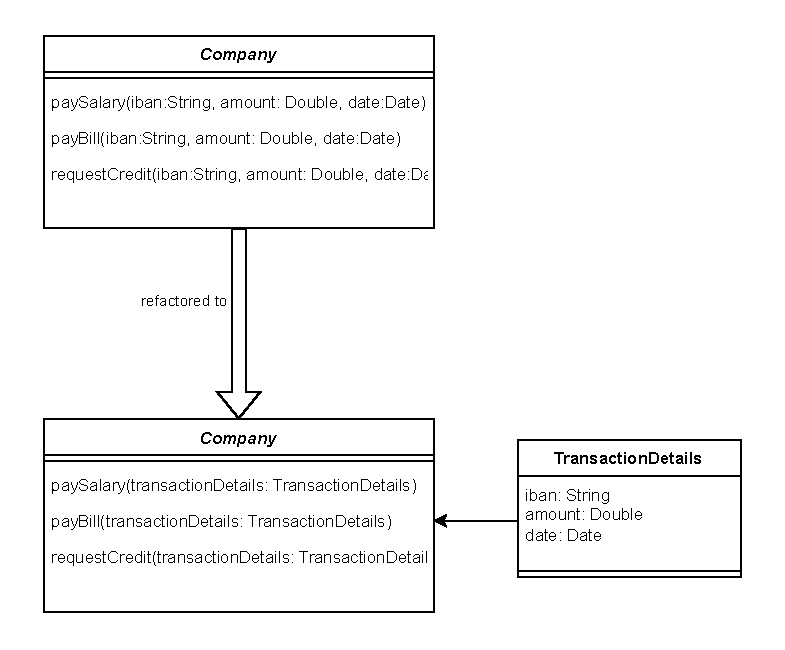
\includegraphics[width=1\columnwidth]{figures/chapter2/dataClump/refactor_simple_case.pdf}
    \caption{The standard approach by extracting a class}
    \label{fig:company_bill_tax}
    \end{subfigure}
       
    \begin{subfigure}[t]{0.4\columnwidth}
        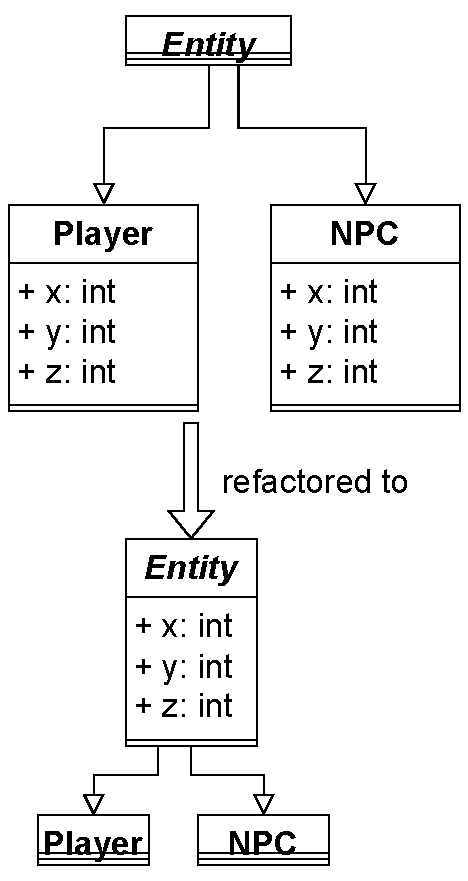
\includegraphics[width=1\columnwidth]{figures/chapter2/alternative_refactorings_move_up.drawio.pdf}
        
        \caption{By moving the fields to the base class}
        \label{fig:move_fields_up}
    \end{subfigure}
     \begin{subfigure}[t]{0.59\columnwidth}
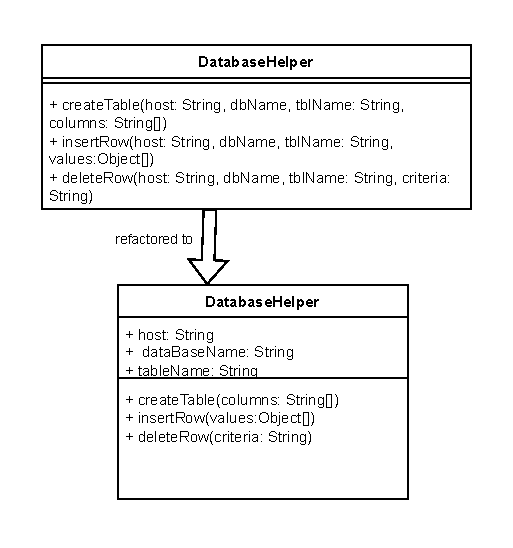
\includegraphics[width=1\columnwidth]{figures/chapter2/alternative_refactorings_to_fields.drawio.pdf}
\caption{By replacing parameters by fields}
\label{fig:params_to_fields}


    \end{subfigure}
\label{fig:refactoring_options}
\caption{Overview of refactoring options of data clumps}
\end{figure}


\subsection{Reasons not to refactor data clumps}\label{sec:data_clump_not_refactor}
As the previous section  outlines, each refactoring option has its drawback and might not be suitable in every circumstance.

Additionally, while data clumps can be classified as a code smell, there are situations where it would be considered not as a code smell or where refactoring is seen unnecessary. 

One reason for not refactoring data clumps is the tendency of producing data classes. These are classes that only provide access to data but no functionality. By extracting a class as outlined in section \ref{sec:data_clump_refactor} the new class has no or scarce additional functionality. These data classes can be also seen as a code smell so that refactoring might not reduce the number of code smells significantly. One way to mitigate this risk can be to further refactor the code by moving functionality related to the extracted class to such class thereby preventing data classes \cite{fowler2019refactoring}. 

Another problem is the creation of those extracted classes is object instantiation. Suppose a method previously requires three parameters \textit{x}, \textit{y}, and \textit{z}. For instance, consider a method that initially takes three parameters: \textit{x}, \textit{y}, and \textit{z}. After refactoring, this method would need just one parameter, an instance of the data class \textit{Point}, meaning callers must now create a \textit{Point} instance instead of providing three separate arguments. This could lead to the creation of many instances, consuming more memory and necessitating frequent garbage collection, thereby reducing performance. While these effects might be minimal, the effect is more significant on embedded systems or other systems with few resources. A similar problem occurs if the access to variables is replaced by getters or setters which also creates some overhead. While many compilers are capable of optimizing such issues, they should nevertheless be considered. 

Also over-engineering can be an issue. As noted in section \ref{sec:data_clump_def}, one can check the existence of a data clump by testing whether the removal of one parameter would make sense. This however is arbitrarily and no concise criteria can be given. Sometimes a group of parameters are connected but an extracted class would create a layer of abstraction that is unnecessary and makes the code even harder to read. This is particular important if the domain of each of the three variables is so distinctive that a common class name is hard to find. 
A popular paradigm in software development is \textit{Don't repeat yourself (DRY)} indicating that code duplication should usually be avoided and abstraction is preferred. However, the counter principle \textit{Write everything twice (WET)} has also gained attention as too much abstraction can hinder readability. \cite{dry}

In modular software projects, extracting a class can cause unwanted or even impossible dependencies.  Suppose a software project has a component for server-related code and for client-related code. Neither of this code is dependent of the other (i.~e. classes in one component are not visible in the other). A data clump connecting those components can only be refactored if the extracted class is located somewhere else. For instance, one could create a \textit{util} package. However, this creates an indirect dependency between server and client code and also might overload the \textit{util} package because it should not contain domain-specific code. 


\subsection{Representation of data clumps}\label{sec:data_clump_graph}

Data clumps can be represented as a graph, so that clusters or pattern can be detected to further evaluate whether a specific data clump is worth refactoring. 

For instance, a graph can be constructed that contains nodes for each class and additionally each method in the software project. If two methods form a data clump, they are connected by an edge in the graph representation. Similarly, two classes  are connected by an edge if there is a data clump relationship between the fields of these classes. 

Another approach is proposed by Baumgartner et al. Here, only the classes that contain data clumps are represented as nodes, and two nodes are connected by an edge if there is a data clump relationship between those two classes. For instance, an edge exists if a method in one class and another method in a separate class are part of a parameters-to-parameters data clump.~\cite{data_clumps_baumgartner}


One approach to represent and serialize data clumps for reporting purposes is the \textbf{Data clumps Type Context} \cite{dataclump_type_context} developed by Baumgartner et al. Each data clump is described by the affected files, classes and methods (if applicable). Additional, the precise location of each data clump is given. Hence,  it employs the first graph representation mentioned in this section, meaning that individual classes and methods are forming the data clump graph. However, the second variant can be re-constructed as well using this information. 
A full description of the format can be found in appendix~\ref{app:data_clump_format}.

To discern one data clump from another, a \textbf{types-names-identifier} is used in this master thesis. This identifier is created by sorting the data clump items by identifier, then joining the data type and identifier of each data clump with a white space, and concatenating these strings with a semicolon. For instance given a data clump \textit{boolean sign}, \textit{int exponent}, and \textit{double mantissa}. The respective types-names-identifier is \textit{int exponent;double mantissa;boolean sign}. This key identifies a data clump based on its types and names thereby helping to find related data clumps. 

The types-names id should be distinguished from the data clump id which uniquely identifies a given data clump. For instance, given a class with three methods (m1, m2, and m3) that share the same three parameters, there are three data clumps with three different ids (m1-m2, m1-m3, and m2-m3), but only one types-name-identifier as all methods share the same parameters. 

With this distinction, sub-problems of the refactoring process can be solved more easily. For instance, finding references of methods affected by a data clump requires that these methods are analyzed separately, therefore the unique id of each data clump must be used to separate the references. On the contrary, finding a suitable class name for a data clump is only dependent on the types and names of the data clump item so that the types-names id can be used. 






\section{Large Language Models}\label{sec:llm}

To successfully use an \ac{LLM}, it is essential to know how it operates and how it should be used correctly to improve the results. This section outlines the relevant background about \acp{LLM}. In the beginning, section \ref{sec:llm_introduction} outlines the technical background of \acp{LLM}. Afterwards, section  \ref{sec:chatgpt}  describes how ChatGPT can be used via the \ac{API} whose structure will be used as the foundation for a general \ac{LLM}-\ac{API} in later chapters. ChatGPT is contrasted to other alternative models in section \ref{sec:other_llm} highlighting that despite the popularity of ChatGPT, these options deserve consideration but have weaknesses too. In the remaining sections, weaknesses and advantages of \ac{LLM} in general are discussed. In section \ref{sec:llm_challenges}, the advantages and disadvantages of using \ac{LLM} are compared giving an overview of what arguments exist on both sides. The succeeding section \ref{sec:llm_considerations} discusses some problems that primarily arise if models are wrongly used and outlines how the quality of these models can be maximized. 


\subsection{Introduction}\label{sec:llm_introduction}
The term \ac{LLM} refers to a machine learning model that can generate and understand texts in an all-purpose manner. 

An \ac{LLM} is trained on a large data set of texts. These texts can come from books, internet pages or other textual sources. The input data is then prepared and sanitized to avoid biases and factual errors.


Then, the training process is performed. By word embedding, the relationship between words is trained such that the model learns the semantic relationship between words. For instance it can learn that cats are animals  or that there is a relationship between men and women. This relationship can be represented as vectors so that for example the relationship \enquote{men to women} can be applied to the term \enquote{king} which results in \enquote{queen}.

Which this training, the model is able to generate coherent texts based on an input that attempts to satisfy any query


For instance, given the text \enquote{How are}, the model  has a access to a corpus of texts where this sentence ends with \enquote{you} so that it is likely to finish the sentence with this word. 

To improve these results, fine tuning is performed. For instance, humans are asked to evaluate the outputs of a \ac{LLM} so eventual errors can be corrected or the model performs better for specific tasks.



Since source code can be viewed as a language, the methods can be applied too. However, specific fine-tuning is needed as source code  has a stricter syntax and a different data set(e.~g. public source code repositories).

It should be noted that a \ac{LLM} still has no sentience. Even if it seems to produce clear and meaningful output, it is still not aware of the inherent meaning. This can result in logical and confident output that is nevertheless wrong. \cite{Amaratunga2023}


\subsection{ChatGPT}
\label{sec:chatgpt}


ChatGPT \cite{ChatGPT_url} is a \ac{LLM} developed by OpenAI and released in November 2022. As a \ac{LLM}, ChatGPT can interpret user queries and return an appropriate response. 

A query can be a question or a prompt directing ChatGPT to answer a question or provide some output. The range of topics ChatGPT can help with is basically unlimited. For instance, ChatGPT can help with math, history, politics, or coding topics. ChatGPT can also understand programming language and therefore, help developers to code.  

The usage of ChatGPT is nevertheless somewhat restricted. For instance, content regarded as hate speech or used for illegal purposes will be suppressed.

Another essential feature of ChatGPT is the ability to store conversations. A conversation is a collection of queries and linked responses sent to ChatGPT. Using conversations, a user can refer to a previous query or response in a later query. For instance, if ChatGPT makes a mistake or misinterprets a query, a user can send another request connected to the previous request and point out the mistake or give more context, helping ChatGPT auto-correct itself. 

ChatGPT can be used via a browser or via an \ac{API}. Using ChatGPT via the browser is free, although restricted. A faster paid version is available and uses an improved model that supports larger ouputs and can process more data.

Figure \ref{fig:chatgpt_browser} illustrates how ChatGPT can be used in the browser.
\begin{figure}
    \centering
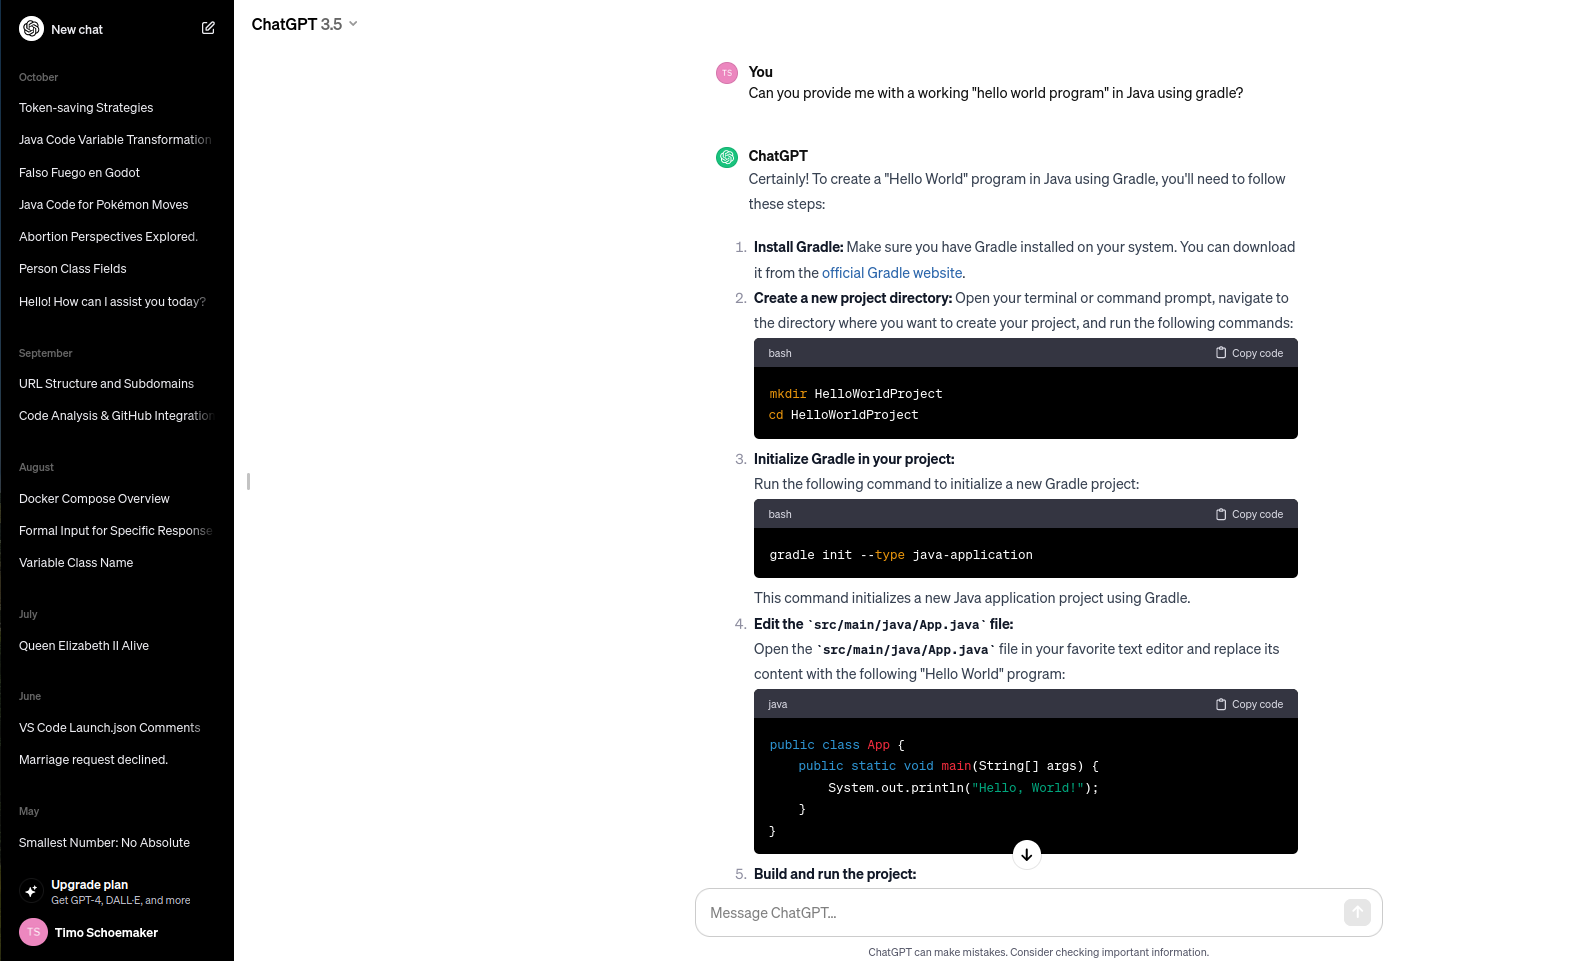
\includegraphics[width=\columnwidth]{figures/chapter2/chatgpt_browser.png}
    \caption{ChatGPT in the browser}
    \label{fig:chatgpt_browser}
\end{figure}
In the main panel that encompasses the most area of the figure, a chat is visualized. This is the the chat with the ChatGPT model. The queries are headlined with \textit{You} and the responses with \textit{ChatGPT}. In this example, ChatGPT is asked to create a \textit{hello world} program with gradle. As a response, the model returned code blocks that the user can simply copy and use. Also descriptions are provided to explain the context and usage of the code.

On the right side, all conversations with ChatGPT are listed. For instance, there is a conversation about \enquote{IntelliJ PSI Modification Fix}. A user can have multiple independent conversations where each has it own context. 

\subsubsection{API}
In order to utilize the ChatGPT \ac{API}, a user has to create an OpenAI account and provide financial information for billing purposes. Each request to the API consumes a certain amount of tokens dependent on the query. 

A token is the smallest unit used by ChatGPT to process a query. For instance, a token could be one English word, a syntactical part of a programming language, a number, or a similar discrete segment of a query. According to OpenAI, a token roughly equates 3/4 of a word, so 100 tokens are about 75 words. However, this is just an estimate for natural language texts in the English language. 

The \ac{API} itself used JSON combined with \ac{HTTP}. For the purpose of this master thesis, only a subset of the available means to use the \ac{API} will be explained because the whole \ac{API} would be too complex and outside the scope this master thesis. 

Listing \ref{lst:chatgpt_api} shows how an \ac{API} query may look like if it used via \textit{curl} which is a tool to  perform \ac{HTTP} requests:

 \begin{figure} [htbp!]
 \centering
			\scalebox{0.8}{\lstinputlisting
			[caption={ Example query to ChatGPT. based on  \cite{ChatGPT_url}}, 
			label={lst:chatgpt_api},
			captionpos=b,language=java, basicstyle=\footnotesize, tabsize=2, showstringspaces=false,  numbers=left]
			{figures/chapter2/chatgpt_api.json}}
		\end{figure}
 

Since ChatGPT uses \ac{JSON} for communication, the content header of \ac{HTTP}  must be set to \enquote{application/json} (l. 2). Subsequently, a token must be provided to ChatGPT (l. 23). which is generated on the OpenAI website and links the query to a specific OpenAI account for billing purposes. It is crucial that this token remains confidential and is not exposed (e.g., through version control systems).

Then, the actual query is defined (l. 4-24.). Firstly, the model is defined (l. 5). OpenAI provides multiple models that have different advantages and disadvantages. For instance, a newer model like \textit{gpt-4} has more capabilities but is more expensive.  By providing a temperature, a user can configure the randomness of the response (l.6). A higher temperature results in more creative answers but this creativity might worsen the quality of the responses. 

Afterward, the actual messages are provided (l. 7-25). Each message is a tuple of a \textbf{role} and a \textbf{content}. The content of a message is the input or output provided to or by ChatGPT. 

The role of a message indicates the source of a message. If the content of the messages comes from a user, the role should be \enquote{user} (l. 13). A reply for a query is defined as the role \enquote{assistant} (l. 17). The system role is a more specific and can be used to include further context for ChatGPT without eliciting a response (l. 9).

The response of the ChatGPT \ac{API} based on listing \ref{lst:chatgpt_api} is displayed in listing \ref{lst:chatgpt_api_response}.
 \begin{figure} [htbp!]
 \centering
			\scalebox{0.8}{\lstinputlisting
			[caption={The response from ChatGPT. Based on  \cite{ChatGPT_url}},
			label={lst:chatgpt_api_response},
			captionpos=b,language=java, basicstyle=\footnotesize, tabsize=2, showstringspaces=false,  numbers=left]
			{figures/chapter2/chatgpt_api_response.json}}
		\end{figure}

In the bottom part of the listing (l.~13-19), meta information is provided. This includes the response generation time (l.~12), the used model for the response (l.~14), and an id for the response (l.~13).

To enable clients to calculate the costs of using ChatGPT, each response also includes how many tokens have been used by the prompt (l.~18), by the response (l.~17), and the total number of tokens (l.~19).

In the upper part of the response (l. 1-11), the actual response is provided. The response is an array of so-called choices (l. 2~-~11). Each choice consists of the actual message (l.~ 6-8), which itself consists of the message content (l. 7) and the role of the content (usually \enquote{assistant}).

The \enquote{finish\_reason} indicates how the \ac{LLM} has finished on the prompt. If the value is \enquote{stop}, the prompt was executed without faults so that the response is valid. If the value is \enquote{length}, the output would exceed the maximum token limit, so the output will be incomplete. The value \enquote{content\_filter} indicates that OpenAI censured the requests because it violates the terms of use of OpenAI. \cite{ChatGPT_url}


\subsection{Other Large Language Models}\label{sec:other_llm}

While ChatGPT is the most known \ac{LLM}, there are several alternatives. This section gives only a broad overview as the focus will be on ChatGPT.

Some recent commercial \acp{LLM} services are Claude~\cite{claude} or Gemini~\cite{gemini}. Compared to ChatGPT, they differ in their training data, context window limitation, or maximum output size. Additionally, their pricing and API usage limits might be more favorable for some users.

A different method  is to use self-hosted \acp{LLM}.
Self-hosting means that the user of a \ac{LLM} has to provide for the infrastructure and resources to run and employ the model. For instance, a separate server could be configured that runs a large language model and listens to requests. This server could be directly set up by the user or rented from another organization (e.g virtual private server). 

With this approach, costs can be saved. Instead of being dependent on the price model of OpenAI which can be subject to changes, the user has to pay for the actual costs (e.g. the monthly rent for a server, the power bills, hardware etc). These might amortize after some years but this is not certain.

Moreover, privacy is more preserved since data does not flow to OpenAI but remains in the control of the user. This is especially important in regions with stricter privacy laws (e.~g. European Union).

A self-hosted \ac{LLM} is also more configurable. There a specific models that have been more intensively trained on coding tasks so that the quality of the results can be improved. The models from OpenAI are more generally trained.  For instance, the \textit{Llama2} model is specialized for human interaction while the \textit{Codellama} is specialized for discussing and generating source code. The \textit{Phind CodeLlama} model is based on the Codellama model and is focused more on the code generation task. 

However, this configuration requires effort and time. Finding a suitable model for a task, installing it, and configuring it is not trivial. For instance, a server needs to be set up that  runs the model, receives queries (e.~g. over a network) and respond back. 

This server must be suitable equipped. In general, at least 32 GB of RAM are necessary. Also video RAM and storage requirements must be met to gain useful performance. These are requirements that cannot be achieved by some users. 




Another problem with self-hosted \acp{LLM} is that they might have lower standards regarding output control. For instance, generating malicious or illegal content is easier with these models than those from OpenAI as they are more censored. 


Self-hosting \acfp{LLM} should not be confused with self-trained \acp{LLM}. In the latter case, a user must train its own model which requires extensive amount of data, even more processing power and the need to properly design the training process to prevent typical issues of machine learning like over-fitting.

\subsection{Advantages and challenges on using Large Language Models}\label{sec:llm_challenges}

While using  \ac{LLM} for refactoring brings many advantages  and possibilities, many challenges should be taken into account. The advantages and disadvantages will be discussed in this subsection. A \textbf{traditional approach} as used in this section means any manual refactoring algorithm (e.~g.,~ refactoring data clumps by extracting a class, removing and introducing parameters in methods, and updating all references)

\subsubsection{Advantages}

First of all, large language models are very flexible. A normal refactoring algorithm needs to consider many situations. For instance, a traditional approach that modifies the method signature in a class might not work on an interface. A large language model does not need to be adapted to all edge cases but often finds a suitable solution to a problem because it is not restricted to a specific refactoring process. \cite{shirafuji2023refactoring}

Additionally, a \ac{LLM} is more similar to a human as it is more  \enquote{creative}. While it is still a computer model and does not win the Turing-Test \cite{turing_test}, a \ac{LLM} can refactor code in a manner more closely as a human being would do. For instance, it can suggest class names that are related to the topic of the class, which a human being would also consider, while traditional approaches would use placeholder names, concatenation of field names or other simple name construction algorithms. \cite{shirafuji2023refactoring}

Large language models are also extensible. For instance, if another programming language is used, an \ac{LLM} can be easily adapted, while a traditional refactoring approach would require more effort to be language-agnostic.

Moreover, a \ac{LLM} can refactor the code in more ways than instructed. While a model can be specifically instructed to refactor data clumps, it might also correct formatting errors, spelling mistakes, or other code smells. While the focus of this master thesis will be on data clumps, other code smells are important too and might be more serious. Using a  \ac{LLM} allows developers to fix more code smells without developing and testing more tools to refactor multiple code smells. As they are better to understand the context of the code than a traditional approach, the quality of the code can therefore be improved. \cite{shirafuji2023refactoring}

Additionally,\acp{LLM} employ a interaction-based learning model which significantly facilitates the integration of developer feedback in real-time. This dynamic learning process allows \acp{LLM} to progressively refine and optimize their suggestions based on continuous interactions with developers. \cite{10.1145/3581641.3584037} 
%Furthermore, \ac{LLM} can adapt to the coding style of the source code. If for instance, the source code used the \enquote{snake\_case} or the \enquote{pascalCase} naming convention, the model can detect this convention and use it for its own refactoring (e.g. creating new methods, variables or classes). A traditional approach would need to be configured for each project to use the right convention so that the generated code might look more artificial as it does not not fit to the rest of the code.


\subsubsection{Disadvantages}

First of all \ac{LLM}s are not trustworthy. They are often confident in their answers which nevertheless are wrong. This confidence can often be broken by asking subsequent questions which lead the \ac{LLM} to rethink the answer. however, doing this in an automatic way is challenging. \cite{azaria2023internal}

Additionally, \ac{LLM} use randomness in their answers which means that the same query can result in different replies. The factors influencing the reply are generally not known and should not be assumed. As a result, requirements regarding a specific output format may be ignored by the model so that developers using a \ac{LLM} must always consider how to parse non-adhering output.  \cite{hu2023large}

One issue that many \acp{LLM} share is hallucination. This means that the model generates a response, but does not come to an end. For instance, an \ac{LLM} generating \ac{JSON} can add more and more \ac{JSON} objects to its response until it has no space left so that it must abruptly stop leaving an invalid \ac{JSON} with no closed braces.  The conditions when such behavior can be observed are unpredictable and should be taken care for. 

Furthermore, \ac{LLM}s are usually black boxes. They do not give hindsight on how they came to a specific reply. While they can explain their reasoning, it is not possible to check the exact thought process.
While a query can consist of multiple parts, conditions, or requirements, a \ac{LLM} will not always adhere to all of these. It may weigh some requirements, ignore other, or interpret them wrongly so that the result is unexpected. A \ac{LLM} may also come to an intermediate result that it will not show at the end even though the intermediate result was correct or requested. Also, no sources of the information is provided. \cite{chen2023instructzero}

Moreover, \ac{LLM}s do not have access to the latest information about a topic. They cannot access external sources like current news and up-to-date documentation. Instead, they employ a so-called cut-off date. Only information before that cut-off date will be used. As of the time of writing this section, the cut-off date for ChatGPT is April  2023. However, the release was several months later.  

There are also security issues with using  \ac{LLM} like ChatGPT. If a model is asked to generate or refactor code, one cannot trust that the code is safe to use. As a result of the cut-off date, the code might use operations that are considered deprecated or even unsafe to use because security vulnerabilities have been detected in the meantime. As a result, the developer needs to verify whether the code is safe to use which is another burden.  \cite{pearce2021asleep}

Furthermore, it is not out of the question that a malicious attacker might change the query or the reply of a \ac{LLM}. Therefore, using such a model might be a feasible way to hack systems or create damage which is difficult to detect and prevent. \cite{not_what_you_signed_for}

Another significant aspect are the legal implications of using \acp{LLM}. Since these models have only recently become mainstream, there are still unresolved legal issues. For instance, since most \acp{LLM} are trained using publicly available data, there are copyright issues as the idea of a particular line of code might come from somebody unknown. Also there are responsibility questions. What happens if the output of the model is malicious or faulty and who is legally responsible for making sure that no damage is done if the output of a model is used. The answers to these issues depend strongly on the jurisdiction. For instance, in the European Union the EU AI Act (Regulation (EU) 2024/1689), requires  transparency for using \acp{LLM} and bans the use of them in situation critical for human safety.  \cite{eu-ai-act}


Lastly, also costs and capacity considerations needs to be observed. For large projects, a \ac{LLM} might be too costly because  the costs are often dependent on the input size. Therefore, the use of large language models should be adequately prepared so that as much costs as possible can be saved.  \cite{chen2023frugalgpt}




\subsection{Consideration while using Large Language Models}\label{sec:llm_considerations}
In order to use a \ac{LLM} more effectively, many considerations should take place beforehand as the quality and potential costs can be strongly affected by them. While an \ac{LLM} can be very flexible and tolerant, ignoring these points nevertheless increases the risk of wrong results. These considerations are  referred to as \textbf{prompt engineering}. 

\subsubsection{Context window and statelessness}

Some \acp{LLM} (such as ChatGPT) are stateless.  This means that the server does not store conversations but delegates this task to the client.  This delegation becomes critical for prolonged interaction with a model. For instance, sometimes it desirable for a user to react to the output of a model by submitting feedback or query about topics that the initial reply does not cover. With a stateless \ac{LLM}, this second query can only be reasonably processed, if all previous messages such as the system message, the user messages, and the associated replies are again transmitted to the model. 


\begin{figure}
  \begin{adjustbox}{minipage=\linewidth,scale=0.7}
     \centering
     \begin{subfigure}[b]{0.3\textwidth}
         \centering
         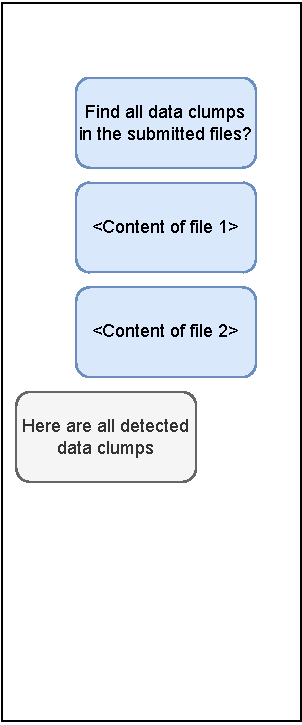
\includegraphics[width=\textwidth]{figures/chapter2/chatgpt_stateless_1.drawio.pdf}
         \caption{Initial request for data clumps}
        \label{fig:llm_stateless1}
     \end{subfigure}
     \hfill
     \begin{subfigure}[b]{0.30\textwidth}
         \centering
         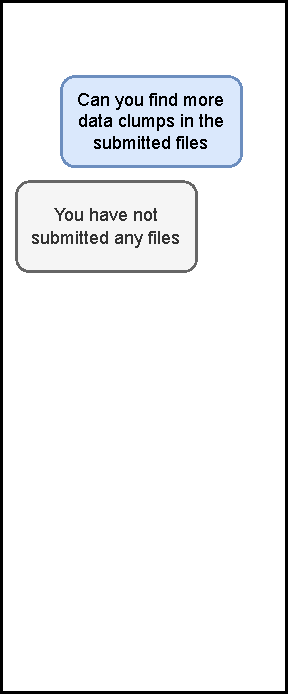
\includegraphics[width=\textwidth]{figures/chapter2/chatgpt_stateless_2.drawio.pdf}
         \caption{Second request without initial request}
         \label{fig:llm_stateless2}
     \end{subfigure}
     \hfill
     \begin{subfigure}[b]{0.3459\textwidth}
         \centering
         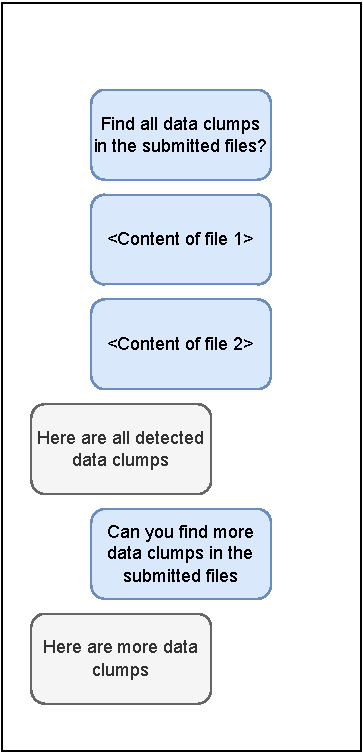
\includegraphics[width=\textwidth]{figures/chapter2/chatgpt_stateless_3.drawio.pdf}
 \caption{Second request with initial request}         \label{fig:llm_stateless3}
     \end{subfigure}
        \caption{Statelessness of \ac{LLM}}
        \label{fig:llm_stateless}
        \end{adjustbox}
\end{figure}

Figure \ref{fig:llm_stateless} visualizes this issue. The dialog with the model is represented as a chat similar to popular messaging programs. Each rectangle represents a distinct message. If it is left-aligned, the message originates from the model (output), otherwise it is a message provided by the user (input). 

In figure, \ref{fig:llm_stateless1}, the user asks a stateless model to find all data clumps in Java files. The \ac{LLM} responds with some data clumps. These might not be all data clumps, so a follow-up request might improve the results \cite{10062688}. Therefore, the user sends another completely new request in figure \ref{fig:llm_stateless2} to instruct the model to find more data clumps. However, the model responds with a general message stating that no files have been submitted. This is the result of the statelessness which requires that the user always send the whole context with each query. In figure \ref{fig:llm_stateless3}, the previous conversation history is provided so that the model accurately responds by finding another data clump.

For models that requires billing, this can be problematic  because the number of required tokens can enormously increase for longer conversations. However, even for self-hosted models, the initial request and the associated responses must be re-analyzed by the model which  consumes a significant amount of resources.


A related issue is the potential to forget information over longer conversations due to the context window. Large language models can only stores a limited amount of information during a conversation. If the amount of information is too large,  a model can react differently. ChatGPT will throw an error so that the user must reduce the amount of information transmitted to ChatGPT.

Other models will forget some parts of it even though they might be relevant for the use case of the \ac{LLM}. Figure \ref{fig:llm_loose_context} demonstrates the issues that arises.  A model is instructed to find and refactor data clumps in java files, and those java files are submitted as well. The response of the model at the bottom of the figure is however unexpected as it only explains the contents of the files submitted. The reason for this response is not some misunderstanding of the prompt but a lack of prompt. The transparent rectangle represents the context window, only covering the content of the transmitted files while the instruction is not covered. 
Because of the context window limitation, transmitting the third file overwrites the content of the prompt so that the model forgets the initial instruction and cannot reasonably process the files, giving instead a description of the files. The problem also arises on greater context window if multiple files or large files are involved as it may be the case while refactoring data clumps.

\begin{figure}[ht!]
    \centering
    \includesvg[width=0.6\columnwidth]{figures/chapter2/chatgpt_context_windows_size.drawio.svg}
    \caption{Example of model forgetting context}
    \label{fig:llm_loose_context}
\end{figure}

Also the output size of an \ac{LLM} is often limited. This means that generating larger text, the model might stop suddenly without finishing the text. In most cases, a \enquote{please continue} prompt can instruct the model to finish its response. The output limits are often reached when the model hallucinates. 
\subsubsection{Choosing the right parameters}
When dealing with an \ac{LLM}, a user must configure the model. The most major settings to be configured are the model itself and the temperature.

In this master thesis, the ChatGPT \ac{API} with the model \textit{gpt-4-1106-preview} is used as it provides a larger context  and output size and supports outputting in \ac{JSON} only. However, the cost associated with this model can be a disadvantage. Alternatively, the model \textit{gpt-3.5-turbo-1106} is cheaper but is not as thoroughly trained. For other providers of \acp{LLM}, other models are available that have their strengths and weaknesses.  

The temperature is another important configurable item. Using a higher temperature can be beneficial for creative tasks. On the other hand, the quality can be worse as the outputs can get more unpredictable. 




\subsubsection{Separate instruction and input}
Many queries to \ac{LLM} include an instruction and an input. For instance, a query to find and refactor data clumps could provide the source code containing the possible data clumps \textbf{(input)}. The instruction could be the query \enquote{Find and refactor all data clumps in this source code}. 

OpenAI recommends that the instructions and input be separated as distinctive as possible. It suggests enclosing the input in a block of \textit{"""} or \textit{\#\#\#} to mark what the input and what the instruction is clearly. For other models, other separation methods might work better as other training data was used but the general idea of this division is always beneficial. 

\subsubsection{Provide detailed context and how the model should respond}

When generating a reply to a query, a language model will use the available context to process the query and generate an output that attempts to satisfy the user's need. This means that every bit of relevant information can help the language model to generate a better response.

On the contrary, providing irrelevant information can increase the chance of wrong responses, so the creator of a query must always consider what to include in a query and what not. 

In the context of data clump refactoring, the query should include the content of the source code and the programming language. However, files that cannot have data clumps (e.g., configuration files) should not be included.

An instruction for refactoring data clumps should state that only the refactored source code files should be returned without providing explanatory texts or other information, as they can hinder the parsing of the output. 

Some models have the advantage of supporting specific output formats which eases parsing
For instance, when using the \enquote{gpt-4-1106-preview} or \enquote{gpt-3.5-turbo-1106} model of the OpenAI-\ac{API}, developers can force the model to respond in \ac{JSON}. Hence, the output can be made more predictable and easier to control. A request using this mode must include the term \enquote{\ac{JSON}}. It should however be noted, that the precise structure of the \ac{JSON} returned may still differ from the request. 


\subsubsection{Chain-of-Thought Prompting}\label{sec:chain of thought}

One way to improve the results from \acp{LLM} like ChatGPT is to separate a query into interconnected sub-queries that lead to a chain of thought. This can be compared to the human thinking process because a human alone tries not to solve a problem at once but breaks it down into simpler problems that are still inter-connected to but easier to solve. \cite{Wei2022ChainOT}

For instance, a query to find and refactor data clumps can be separated into a detection query and a refactoring query. These sub-queries can be further divided into a query for each file or for all files in a single directory. As a result, not one a single query is needed but multiple queries. 

This is useful if a human is reviewing the output from a \ac{LLM} since obvious errors can be spotted more easily if the task is divided into multiple steps. However, it is more challenging for an automated tool since it cannot find errors in the same way. 

Furthermore, one should consider that each queries requires further overhead so that the performance might be impacted more negatively. 





\begin{comment}
\subsubsection{Hosting a large language server}

One method to host a \ac{LLM} is via \textit{Ollama} \cite{ollama}. Ollama is a program to download, configure, and host a local \ac{LLM}. Users can set up a large language model with one command and query the model via the command line or a \ac{HTTP} interface.



After a model has been downloaded, a user can execute the command \textit{ollama run <model>} to submit queries 

Similar to to ChatGPT, there is an \ac{API} to integrate Ollama in other application. After installed, Ollama listens to \ac{HTTP} connections  on localhost and port 11434.

Listing \ref{lst:ollama_request} shows how such an \ac{API} can be used via \textit{curl}.

The difference to the ChatGPT \ac{API} are scarce. In contrast to ChatGPT, there is no header for an authorization token because no direct payment to any organization is needed. 

Additionally, Ollama streams replies by default meaning that not the full response is returned at once but multiple response parts that must be aggregated by the user. As this is not useful in the context of this master thesis, it is disabled by setting stream to false (l. 11).

Moreover, another model is used (l.~4) as the ChatGPT models are not available. 


 \begin{figure} [htbp!]. 
			\lstinputlisting
			[caption={ Example query to ChatGPT  \cite{ChatGPT_url}},
			label={lst:ollama_request},
			captionpos=b,language=json, basicstyle=\footnotesize, tabsize=2, showstringspaces=false,  numbers=left]
			{figures/chapter2/ollama/ollama_request}
		\end{figure}

  \end{comment}
\section{Related work}\label{sec:related_research}
The problem of data clump detection and refactoring is addressed in multiple papers. Also the  use of large language models in software development is a fairly recent rearch topic. In this section, research to both topics will be outlined: 

\subsection{Related to data clumps}
Baumgartner et al. developed a live code smell detection plugin for IntelliJ that can detect, report, and refactor data clumps without significantly impacting performance. However, the tool is semi-automatic, meaning the developer must still actively approve the data clump refactoring and suggest a suitable class name for the extracted class. \cite{BaumgartnerAP23}

As outlined in section \ref{sec:data_clump_def}, the definition of data clump by Fowler \cite{fowler2019refactoring} is somewhat ambiguous because no clear criteria to determine data clumps is established. Zang et al. \cite{zhangImprovingPrecisionFowler2008} creates a more algorithmic approach to determine whether a data clump exists. This approach is also explained in section \ref{sec:data_clump_def}. The authors also provide more precise definitions of other code smells like \enquote{message chains} or \enquote{speculative generality}. By interviewing four software development experts about the code smell definitions the authors developed, they find that their new data clump definition receives relatively more disagreement than other definitions, which the authors explain are the results of not covering edge cases in the definitions. 


Hall et al. analyzed the impact of code smells (including data clump) on the occurrence of faults in three open-source software projects. They find that data clumps have a mixed correlation to faults because, in two of the three projects analyzed, the correlation of data clumps per \ac{LOC} to detected faults is negative for two projects and positive for one project. This rejects their hypothesis that data clumps do not affect faults, and the authors suggest that the application domain and the development context need to be considered before the time-consuming refactoring of data clumps since their impact is not predictable.  \cite{hallCodeSmellsHave2014}


Murphy et al. \cite{stench_blossom} developed a visual tool to find code smells (including data clumps). the tool named \textit{Stench Blossom} is a plugin for Eclipse. If a plugin user views a file, the tool searches for code smells and displays them at the right side of the eclipse editor. Each code smell is visually displayed as a a \textbf{petal}. The radius of such petal represents the strength of a smell (i.~e. how strongly violates the code smell the given coding guidelines). The petal has a color that indicates how obvious a code smell is. Orange code smells are not very obvious while blue code smells are easy to detect by human beings. Since orange has a closer connection to warnings, it is more easily to perceive so that undetected code smells can be fixed better. Experiments with \textit{Stench Blossom} shows that the median number of code smells detected by humans using the tool increased from 11 to 21. However, data particular for data clumps is not given.  

\begin{comment}
Neto et al. developed an agent-based platform to detect and refactor code smells (including data clumps). The platform uses everal agents that work regularly to fix code smells. Each can obtain norms that describes what code smells it should fix, what conditions 
\end{comment}
\subsection{Related to large language models in software development}

White et al. \cite{White2023ChatGPTPP} outline how ChatGPT can be used in software development to improve the worklflow of developers. This includes  exploration of requirements, removing ambiguity in technical specification, or describing source code. The authors suggest specific prompts to elicit a suitable response from ChatGPt.

In case of refactoring, the author suggest that ChatGPT is able to refactor code with multiple prompts. For instance, ChatGPT can refactor based on a well known design pattern name, multiple examples on how to refactor the code, or a more lengthy requirements description. The exact success of each prompt is however dependent on how ChatGPT is trained and should be scrutinized manually. 

Cao et al. \cite{cao2023study} focus on using ChatGPT for fixing deep learning programs. Those are programs that cannot be understood only by their source code alone, but are are largely influenced by underlying data like  neural networks etc. This makes finding faults more difficult. The study finds out that ChatGPT can find code smells and detect faults. Without giving instructions however, ChatGPT will tend to return code smells and outdated API calls while not finding other bugs. 

\subsection{Refactoring tools}

\subsubsection{ Program Structure Interface}\label{sec:psi}
The Program Structure Interface provided by IntelliJ is an \ac{API} to analyze and modify  projects that the \ac{IDE} \textit{IntelliJ} can load. As a result, the various classes, methods etc. can be obtained which allows for the detection of data clumps. Also modifications are possible so that data clumps can be refactored.

In order to use this API, an instance of IntelliJ must be started. IntelliJ can be started in a headless mode to reduce loading times and improve the performance so that no GUI is initialized. Nevertheless, IntelliJ requires many resources and much overhead, so that  the initialization needs some time.

\begin{comment}
\section{Related work}
Since refactoring code smells is becoming increasingly important for developers, a variety of research has been conducted to study how the refactoring process can be improved.

Furthermore, tools have been developed that on their own cannot refactor code smells but can be adapted and used to ease developing refactoring tools.

Additionally, the use of \ac{LLM} in software development has recently gained widespread attention and has become a focus of several studies which analyzes the potential and challenges in practice. 

\subsection{Tools to assists data clump refactoring}





\end{comment}


\clearpage
\begingroup
\renewcommand{\cleardoublepage}{} % TODO maybe removing this and next
\renewcommand{\clearpage}{}
\chapter{Concept}\label{chapter:conception}
\endgroup
This chapter deals with the design of the program. It provides information about the processing pipeline (\ref{sec:pipeline} and how the different parts of that pipeline can be modeled in a way that allows easy extension. This is expanded by the context that stores the data of each step (section (\ref{sec:context}). Then, the integration of \ac{LLM} like ChatGPT will be analyzed. 



\section{Pipeline}\label{sec:pipeline}
In order to find and refactor data clumps automatically, a particular sequence of steps \textbf{(pipeline)} has to be respected. Most steps of this sequence must be in a specific order because they rely on information extracted in a previous step. 

This section outlines the structure of the pipeline. Section \ref{sec:pipeline_structure} gives an overview of how the pipeline is implemented. 

Section \ref{sec:pipeline_exec_order} discusses an alternative but similar approach for the pipeline which is relevant if multiple data clumps are considered in the pipeline. 

Finally, section \ref{sec:pipeline_steps} describes each important pipeline steps and what considerations should be taken into account when developing tools for the respective pipeline step. 


\subsection{Structure of the pipeline}\label{sec:pipeline_structure}
Each step of the pipeline is performed by a  \textbf{handler}. A handler might handle one or more steps.  Each handler has information about what steps of the pipeline it supports and  a handler can be registered to a pipeline step if it supports that particular step.  

Since a service-based approach is used, a handler can be seen as a gateway to a different program or service that performs the specific functionality.  The handler and the respective service are tightly coupled. Although a handler could manage multiple services, this is not a design requirement and must be handled with care. Nevertheless, it is recommended to write the handler as abstract as possible.
\begin{figure}[ht!]
    \centering
    \includesvg[inkscapelatex=false,scale=0.9]{figures/chapter3/solver_gateway_service.svg}
    \caption{Visualization of communication to services for one pipeline step}
    \label{fig:solver_gateway_service_overview}
\end{figure}

Figure \ref{fig:solver_gateway_service_overview} illustrates how the service-based approach works for one step:

\begin{enumerate}
    \item The program developed in this master's thesis \textbf{(main program)} executes one step (e.~g. finding a suitable class name)
    \item The handler registered to that step is used. It is provided with the current context containing the results from previous steps.
    \item The handler starts or employs a specific service. This service might be dependent on the current step or might be constant. The handler knows how to start or use the service and sends all relevant information to the service (e.~g. via files, network streams etc.). 
    \item The service processes the requests submitted by the handler. For instance, ChatGPT can suggest a suitable class name. The service might be outside of the control of the developer. For example, it might be programmed in a different programming language or the source code might not be available. At some point it will create a response and send it back to the handler. 
    \item The handler reads the response and processes it. It then creates a new context based on the previous context and the response from the service. 
    \item The new context is returned to the program and can be used for successive steps (e.~g. the suggested name can be used for creating a respective class) 
\end{enumerate}



A handler can also check whether it can be run in the given situation. For instance, a code obtaining handler can determine whether the project location does in fact exist or a validation handler for \textit{Gradle} can check whether the project is indeed \textit{Gradle}-based.

The program, therefore, acts as an orchestrator. It starts every service and controls them. The steps and services are temporally coupled. A step cannot be started unless all previous mandatory steps have completed. In most cases, if a step was not successful, further execution of the pipeline makes no sense, so it can be aborted. 

An alternative approach is called choreography. Here each step would call the next step without using the central main program. 

Both approaches have their advantages. In the choreography architecture, there is less coupling since a main program does not need to know which handler is associated with which step. Instead, each handler need to know the next (and only the next) step. This can become challenging if steps are optional because the gateway does not know what service to call next. Additionally, debugging the process is more challenging as there is no central point that coordinates the pipeline.

On the other hand, the orchestrator architecture is easier to control and debug. It is easier to configure and to implement. Nevertheless, the coupling to each handler is stronger because each gateway must be known by the main program. Additionally, the main program is a single point of failure. If there is a problem with the main program, the data clump refactoring cannot proceed as every step requires coordination with the orchestrator. Also the overhead should be considered because the orchestrator will need to act multiple time to process responses and generate new requests for the next gateway. This issue gains importance if services are remote, accessed via the internet or a local network, thereby increasing overhead. \cite{orchestration_choreography}


\subsection{Pipeline execution order}\label{sec:pipeline_exec_order}

Another issue to analyze is the pipeline execution order. This should not be confused with the pipeline step execution order. The latter is simply the order of the different steps (e.~g. code obtaining before data clump detection). 

The former order deals with how the steps are executed with respect to each detected data clump. Two approaches are considered here:

In the first approach, each data clump is  further processed immediately after detection. This means after a data clump has been detected, it is immediately given a suggested name, a class is extracted if necessary, and the refactoring is executed. In the following, this approach will be referred to as \textit{one-data-clump approach}.

In the second approach, all data clumps are detected first. Then all, those data clumps are assigned a suitable name, and classes are extracted if necessary. At the end, each data clump is refactored. In the following, this approach will be referred to as \textit{one-step approach}.

As a result, in the \textit{one-data-clump approach}, a data clump is processed by one step of the pipeline and then by the next while in the \textit{one-step approach} the first step has to process all data clumps first before the data clumps can be processed by the succeeding steps.

There are arguments for and against both approaches. However, designing a system that supports both approaches is challenging and out of scope for this master's thesis, so only one approach is used. 

The \textit{one-data-clump approach} leads to quicker intermediate results so that if the tool to be developed is stopped during execution, it is more likely that some data clumps are fixed so that some progress is being made.

Additionally, this approach is better for load balancing. Since many services might be used for refactoring data clumps and one data clump is processed at a time, each service gets a longer break before being used again. This is  especially important for services like ChatGPT, where many requests in a short time period can lead to outages or huge costs. 

On the other hand, the \textit{one-step approach} is easier to implement using the tools already existing. For instance, the \textit{DataClumpDoctor} detects all data clumps at a time and therefore is more compatible with the \textit{one-step approach}.

Moreover, configuration mistakes can be fixed more easily because in this approach, the software project will not be modified for some time (i.~e. data clumps will be detected or suitable names will be found). As a result, users of the tool are more likely to safely stop the tool if they discover a configuration mistakes. This might often occur in the very first moments after starting the tool.

Additionally, this approach can use the cache more efficiently. Since one service is being used  over a longer period of time,  relevant data for the service can be cached better in contrast to switching the service frequently  As a result, the performance can be increased. 
\subsection{Pipeline steps}\label{sec:pipeline_steps}
In the following subsections, the steps of the pipeline will be outlined. For each step, there is a discussion on why this step is noteworthy to consider and what points are important when implementing the step.
\subsubsection{Code obtaining}\label{sec:code_obtaining}
Data clumps can only be found if access to the source code is given. This requires that the source code is available in some location and that the location is known.

In most cases, this is trivial since a developer needing to find and fix data clumps should know where the source code is located.

However, there might be more complex cases. For instance, the source code could be located on a \ac{VCS} or must be fetched elsewhere so that the newest changes can be included. Therefore, defining a specific step for obtaining the source code before proceeding with the rest of the pipeline is useful. 


\subsubsection{File filtering}\label{subsub:filtering_files}
After retrieving the project files, a file filtering process is important. A software project consists of many artifacts like actual source code, images, libraries, or other resources. For this master thesis, only source code files are pertinent for data clump detection. 


However, not every source code file might be analyzed for data clumps. For instance, parts of the projects must not be refactored, or a re-factorization would be too time-consuming. As outlined in chapter \ref{sec:introduction}, the cost of detecting data clumps might need to be minimized. Therefore, filtering rules might be necessary to reduce the scope of the files that are considered in the the subsequent steps.  

File filtering can be achieved through several methods:

With pattern-based filtering, inclusion rules and exclusion rules can be used to filter out irrelevant files.  To facilitate these rules, regex patterns can be used.  Each inclusion pattern specifies which file must be included, and each exclusion pattern specifies files that must be excluded. For instance, consider \textit{includeGlobs=[\enquote{.*\.java}]} and \textit{excludeGlobs=\enquote{.*Main.java}}. In this case, all Java files are included, if however a file ends with \enquote{Main.java} it is excluded.

The precedence between include and exclude rules can have a major impact on defining the correct rules. In the example above, exclusion rules override inclusion rules.  This means that few files can be excluded with few exclusion rules. If however only a small set of files should be considered while excluding a larger set of files, this prevalence should be reversed so that inclusion rules dominates over exclusion rules. In this master thesis, the latter approach will be chosen due to its  compatibility with programs like PMD and its ability to simplify partial analysis of software projects. 

More complex filters can also be used. For instance, only considering files changed by the latest commit or rank the files given a specific metric and keep the best files. Details of these more complex filtering methods can be found in section \ref{sec:data_clump_filtering}
\subsubsection{Extraction of AST}
Then,  the source code needs to be simplified as comments, the method bodies, and other language parts are irrelevant for detecting data clumps. This could be achieved by extracting a subset of the \ac{AST} from the source code, which includes all the relevant information to identify data clumps.


\subsubsection{Data clump detection}
This step is among the most critical of the pipeline. 
The handler finds all data clumps given the filter constraints established before and returns a new context with the description of the detected data clump in the format suggested by the \textit{DataClumpDoctor}. 

The handler should take care that it only finds data clumps, and not related parts of the source code. For instance, finding where a data clump method is called is not part of this step and should not be saved yet. 

Moreover, each data clump must receive an unique ID. While the structure of this ID is not relevant and does not need to be parsed, concatenating the available information of the data clump (e.~g. class name, data clump items) is a suitable way to generate such an ID

\subsubsection{Data clump filtering or prioritization} \label{subsub:filtering_data_clumps}
In section \ref{subsub:filtering_files}, a filtering by files is performed. However, even if many data clumps were detected, they do not always need to be refactored. One can decide to ignore certain data clumps and refactor them later or even never. 

There can be many reasons for this approach. For instance, parts of the source code that are infrequently updated might be too risky for refactoring since any automatic tool might cause bugs or invalid code that is hard to fix because the developers are unfamiliar with this part of the source code. On the contrary, a part of the source code that is updated more frequently might be in an intermittent state, so that refactoring is currently not recommendable. Also, as noted in section  \ref{subsub:filtering_files}, if a service like ChatGPT is used, the cost of transferring many source code files with data clumps might be too high. 


Therefore, filtering out certain data clumps considered not worthy of refactoring can be suggested.

There are several methods to filter out data clumps which will be discussed in section \ref{sec:data_clump_filtering}

\subsubsection{Name finding}\label{subsec:chap3_data_clump_name_finding}
The next step of the pipeline is to find a suitable identifier of the extracted class.

There are some criteria for this identifier. It should be a valid name in the respective programming language so that, in general, only alphanumerical characters may be chosen. It should not conflict with other identifiers as it may lead to bugs or compiler errors, and it should be readable and, as best as feasible, represent the fields of the class.

Hence, the name finding is a complex process requiring domain knowledge and creativity if the resulting name should be acceptable. 
Since English is the predominant language of identifiers, it will be assumed that only English identifiers will be used. 

\subsubsection{Reference finding}
 Having detected a data clump, there is still information missing to refactor it. In particular, successful re-factorization requires that every method call, method definition, variable usage or variable definition that is connected to the data clump is updated in a later step. These so-called \textbf{references} need to be found so that they can be updated.

Since the identifier of the data clump variables (or methods) is known, one could search for all occurrences of that identifier. This, however, is not enough because identifiers have a scope. A variable with the name \textit{var} can be declared as a field, as a parameter of a method or inside a block (e.~g. if-branch). Each of these names can refer to different variables although they have the same identifier. As a result, a textural replacement approach will not work consistently.

Therefore, additional tools will be needed to parse the source code and use the rules of the programming language to find where the data clump items are indeed used.
\subsubsection{Class Extraction}\label{subsec:chap3_data_class_extraction}
After a class name has been found, a respective class can be added to the source code. This class will be used as a replacement for the data clump variables or parameters. 

In contrast to the name finding step of the pipeline, this process can be automated more straightforwardly because it does not require creativity and a general template can be used, that is:
\begin{itemize}
    \item Create a private field for each variable of the data clump
    \item Create a public getter for each variable of the data clump. This getter may be named \textit{getVar} where \textit{Var} is replaced by the capitalized name of the variable. The method returns the value of the respective field
    \item Similarly, a setter \textit{setVar} may be created that has no return type, accepts a new value as a parameter, and sets the respective field. 
    \item A constructor that initializes the fields with provided or default values may be created. 
\end{itemize}

Additionally, methods for converting an object to a string, checking the equality of two objects, or creating a hash code may be useful, but these methods are usually optional for refactoring data clumps. 


\subsubsection{Refactoring}
After extracting a class, the next step is to refactor the source code to remove the data clumps. Here, again, one needs to differentiate between method parameter data clumps as this impacts the access scope. 

In case of a field data clump, the following transformations need to be applied.

\begin{enumerate}
    \item For each class in which the same field data clump is detected, the data clump variables are replaced by an object of the extracted class
    \item A getter of that object is created that has the same access level as the highest access level of the data clump items
    \item If a data clump item is read, it must be replaced by a call of the respective getter of the extracted class
    \item Similarly, if a data clump item is written to, the assignment must be replaced by a setter
\end{enumerate}



In the case of a method data clump, the general approach is similar to the case of field data clumps. An object of the extracted class replaces the data clump items, and all references to the data clump items are also updated. Additionally, the calls to the refactored method must be updated. Instead of providing the arguments for the data clump items directly to the method, an intermediate object can be created that is filled with those values, and this object is provided to the method. 

\subsubsection{Validation}

At the conclusion of the refactoring process, it is not certain that everything is perfect. This applies to manual refactoring and also to automatic refactoring. For instance, there might be an undetected error, the refactoring leads to ambiguous method signatures, some reference are not up-to-date etc.

As a result, it is critical to test the project after refactoring so to make sure that all requirements are still fulfilled. Testing includes checking the project for build errors (e.~g. invalid syntax, missing dependencies etc.) and unit test, where the functionality of the project is tested. Since those unit tests are supposed to run quick, they should be included in the validation check. 

Many build systems like \textit{Gradle} or \textit{Maven} support simple commands to run all unit tests and build the project in a consistent manner.  Therefore, one can run such a command and check the exit code or output to determine whether the project compiles and passes unit tests.

Disadvantageously, this may only be effective if the project is correctly configured with a build system. This might not always be the case, and it is not trivial to construct an interface for a general build solution. 

\subsubsection{Evaluation}

As another optional step, one might evaluate the effectiveness and efficiency of the data clump refactoring. For instance, one could execute the data clump detection process again to determine how many data clumps are fixed in comparison to the first iteration. 

Another metric for the evaluation could be the running time. A substantial running time of the refactoring can slow down the development process and cause the program not to be used again for future iterations. It could also be useful to analyze the running time for each individual step so that handlers that require too much time or resources can be detected and later not be used. 

\subsubsection{Committing}

After all changes are made,they  are still local and not part of the \ac{VCS}. As a result, they must be committed and pushed so that every developer of the software project has access to the changes by the refactoring. Hence, it can be viewed as the reverse of the code obtaining step. 

In this step, a suitable commit message should be chosen. This could also be done via ChatGPT.    Also a manual message based on the changed files might be sufficient. Further issues that might arise is whether a new branch should be created for the refactoring and how humans or other automatic tools (Continuous integration continuous development) should be used to validate the refactoring.  
\section{Context}\label{sec:context}
In section \ref{sec:pipeline_steps}, the several steps of the data clump pipeline are outlined. However, these steps do not include how the information generated by each step is stored and how successive steps might use this information.

Therefore, a concept to store intermediate information needs to be developed. Such information might be called \textbf{context}.


Section \ref{sec:context_structure} gives a broad overview of how the context is implemented.

The serialization of the context which is important to persist the data of the several steps is then outlined in section \ref{sec:context_serialize}.

Finally, the most important context data types used by the tool are discussed in section \ref{sec:context_steps}.

\subsection{Context structure}\label{sec:context_structure}
The context is a  dynamic repository filled throughout the data clump refactoring pipeline. The context can be represented as a linked list. Each node of the list encapsulates a distinct segment of the context which is an extension of the previous context. In the beginning, there is no context and the code obtaining context is created.

When a handler needs to access information from a specific context, it needs to traverse the linked list until it finds the needed information. 


Each step in the data clump refactoring pipeline can access the context and obtain such information as it may deem necessary for its use. A step may or may not update the context. For instance, if a service performs multiple steps consecutively, it does not need to share  some information, or this would be harder to implement. To give a more concrete example, if a service can find data clumps and refactor them automatically, it might not be able to store the locations of each data clump so that respective context cannot be created. Also, a handler can create multiple chained contexts if it is capable of executing multiple steps. 




Figure \ref{fig:context_pipeline} illustrates how a different combination of handlers can affect the state of the context. The figure depicts three state diagrams where rectangles visualize the most recent context and arrows indicate executed steps.  In figure \ref{fig:context_pipeline1}, the \ac{LLM} performs the detection of data clumps, and the refactoring (including all associated sub-tasks). Because all these tasks are performed by the same service, it would be unnecessary to save intermediate results. Therefore, the context is only updated once at the conclusion of the program. This final context does not have additional information but marks that the pipeline has been executed successfully.
 

\begin{figure}[H]
\centering
  \begin{adjustbox}{minipage=\linewidth,scale=0.7}
     \centering
     \begin{subfigure}[b]{0.3\textwidth}
         \centering
         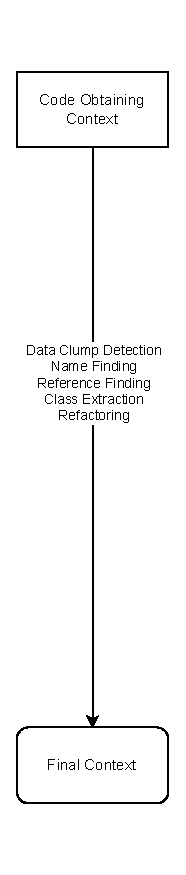
\includegraphics[width=\textwidth]{figures/chapter3/context_pipeline_1.drawio.pdf}
         \caption{All steps are performed by an \ac{LLM}}
        \label{fig:context_pipeline1}
     \end{subfigure}
     \hfill
     \begin{subfigure}[b]{0.30\textwidth}
         \centering
         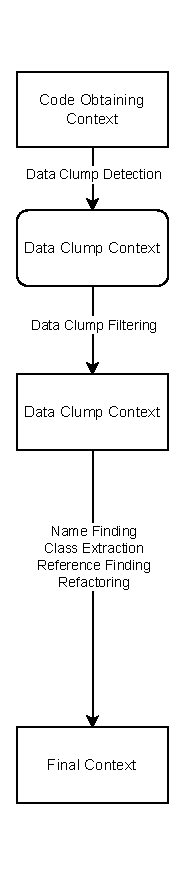
\includegraphics[width=\textwidth]{figures/chapter3/context_pipeline_2.drawio.pdf}
         \caption{Detection and filtering by another tool}
         \label{fig:context_pipeline2}
     \end{subfigure}
     \hfill
     \begin{subfigure}[b]{0.3\textwidth}
         \centering
         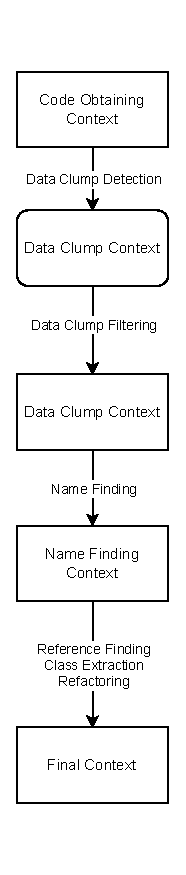
\includegraphics[width=\textwidth]{figures/chapter3/context_pipeline_3.drawio.pdf}
 \caption{Only name suggestion by an \ac{LLM}}         \label{fig:context_pipeline3}
     \end{subfigure}
        \caption{Exemplary lifecycles of the context}
        \label{fig:context_pipeline}
        \end{adjustbox}
\end{figure}

In figure \ref{fig:context_pipeline2}, some parts of the pipeline are performed by the \textit{DataClumpDoctor} and other programs. For instance, data clumps are detected by the \textit{DataClumpDoctor}. As a result, a data clump detector context is created containing all detected data clumps. Afterwards, a filter removes non-important data clump and creates a new context of the same type that is linked to the previous context. If a later handler requires information about the detected data clumps, it needs to find the first context that contains this information  beginning at the tail of the linked list. In this case it would be the filtered data clump context, not the original data clump context. Here, also the context is not updated after the filtering process as the rest of the work is performed by an \ac{LLM}. 

In figure \ref{fig:context_pipeline3}, the context is extended by a name finding context. This context includes information about a suitable identifier suggested by a \ac{LLM}. A manual refactoring tool (e.~g. IntelliJ), can use this context to perform the refactoring without further input by an \ac{LLM} so that the role of the model is limited here. 




To check whether a given pipeline is indeed executable, each step handler must describe how the context is updated when the step is executed. Each step can also specify whether a specific type of context must exist. For instance, a step may require that the \ac{AST} is available for a given source code file. 


\subsection{Context serialization}\label{sec:context_serialize}

One advantage of developing a shared context is that it can be serialized  and de-serialized with less effort. At every step of the pipeline, the current context can be  serialized into a specific location. If for some reason, the pipeline could not be executed successfully or the user of the tool is not satisfied with the result, the program does not have to be re-run, but previous results can be re-used. This is particular important in the case of persistent handlers like the \textit{DataClumpDoctor}. Re-running this service multiple times under the same parameters would have no advantage but consume resources and time. By serializing the data clump detection results, the data can be retrieved again without executing the tool again.

Another benefit of serialization is that the context can be transmitted to services easily. For instance, the service can be given the path of the serialized context which it can load. This eases communication with service  but requires that the service can understand the serialized context. 

Also, for \ac{LLM}-related steps this can be useful because every call to an \ac{LLM} induces costs. On the other hand, however, the creativity and randomness of such models can be an argument not to de-serialize such results but re-generate them so that multiple proposals can be created.



In the end, the issue of whether to use context serialization or not should depend on the service and also should be configurable by the user of the tool. 

\subsection{Context information per step}
\label{sec:context_steps}
\begin{comment}
In the following, the context created or updated after each step will be explained:

\subsubsection{Code obtaining}
The context after obtaining the source code of the project to analyze is usually the path to the project after it. In most cases, the project is defined in such a manner that there is a single base directory under which all files and directories of the project are located.

Alternatively, one could store the list of all relevant file paths of the project. This requires more storage but makes it easier to filter out files. 

\subsubsection{File Filtering}
Developing a filtering context is more challenging. One major issue is that services suitable for data clump detection offer varying solutions for including and excluding specific files. For instance, PMD which is used by the \textit{DataClumpDoctor} requires that a rule set file is located at a specific location. This rule set file contains inclusion and exclusion rules using regular expressions. 

If files are sent to an \ac{LLM}, the filtering can be performed directly on the handler level, so that more sophisticated  filtering rules can be applied without being restricted to use regular expressions. 

Because the pipeline design separates the context from the handlers, the context has limited information about the handlers and does not know which handler will be executed later. Therefore, the filtering context must be very general to maximize compatibility with all possible handlers. 

Therefore, as a design decision, the file filtering context contain only file inclusion and exclusion rules that can be applied by subsequent handlers. This means that a more complex filtering rule (e.~g. by commit date), must be resolved to a list of files to be included and excluded. 

It should also be noted that inclusion and exclusion rules might conflict, and these conflicts can be handled differently. In the case of PMD, if a file is included and excluded according to the rules, the inclusion prevails so that it is included. This makes it easier to only include a limited set of files and exclude a large number of other files. Vice versa, it is more challenging to exclude a very limited amount of files while including more files. The file filtering context does not attempt to resolve these issues. 


\subsubsection{Data clump detection and filtering}

The format described in appendix \ref{sec:data_clump_format} can be used to store the detected data clump. While this format is relatively new, it contains all relevant information for storing data clump information and is extendable. The same format can be used for filtering too as all irrelevant data clumps can be removed easily. As a result, this context is an example of a context that might appear multiple times in the linked list. 

\subsubsection{Name finding}
To store the determined names per found data clump, a dictionary can be used that maps the types-names-identifier of the data clump to a name.

One possible extension for this context could be to store multiple name suggestions for a given data clump. However, this is not part of the modeled pipeline as the benefits do not outweigh the increased complexity.

\subsubsection{Class path choosing}

At the class extraction step, the created class must be saved somewhere to be considered part of the project. The exact location can significantly impact the readability of the source code, as the location of files in a software project can help in understanding the project. 

For instance, the class could be where the data clump is initially found. This can lead to arbitrariness as the exact order of where and when data clumps are detected might not be predetermined. It should also be noted that there are always at least two parts of a data clump (e.g. two methods). As a result, if the two parts are located in separate directories, it is difficult to determine where the extracted class should be located. 

Alternatively, specific locations can be used to store all extracted classes. This, however, can also hinder readability as the extracted classes have no connections to the places where they are used. 

As an alternative, the complete class body could be stored instead of saving it directly to a file. This might be advantageous if the class content should be formatted, refactored or otherwise modified in order to be valid. This also would deflect the responsibility of the class location from the class extractor step. 

For this master's thesis, the first approach is used. The type-name--key is mapped to a specific path which is chosen at the name suggestion step although it could also be chosen at the class extraction step. 

 
\subsubsection{Validation}

The validation step context requires at least information about whether the validation is successful (i.~e. no compiler errors occur and all unit tests pass). 

In case of a failed validation, one might need more information. For instance, it is helpful to know which unit test fails or on which line the code fails to compile. In many cases, modern build tools like \textit{Gradle} already acquire these data so they can be easily obtained. These error information can then be used to correct errors. 


\end{comment}

\begin{table}[ht!]
    \centering
    \begin{tabular}{m{3cm}|m{2cm}|m{5cm}|m{2cm}}
        Name & Generated in step & Contained data/methods & Serializable?  \\\hline
        Code obtaining & "" & Path to project & No \\\hline
        Git repository & Code Obtaining & Timestamps of changes in files, recently changed files & No \\\hline
        File filtering & "" & Include, exclude expressions, flag whether inclusion prevails over exclusion & No \\\hline

        AST & "" & \ac{AST} for each analyzed file &  Yes \\\hline
         Data clump detection & Data clump detection/filtering  & Format described in appendix \ref{app:data_clump_format}, generation of types-names-keys & Yes \\\hline 
         Name finding & "" & Names for each types-names-key & Yes\\\hline

         Class path & Name finding & Class paths for each types-names-key & Yes\\\hline

         Usage finding & "" & For each data clump: type of usage and  location & Yes \\\hline

         Validation & "" & Building successful?, error information & No \\\hline
         
    \end{tabular}
    \caption{Most important context types}
    \label{tab:context_types}
\end{table}

Table \ref{tab:context_types} shows the main context types that are created and used until the pipeline finishes. It shows the pipeline step in which the context is usually created, the operation and data it contains, and whether the context can be serialized (and hence deserialized). Quotes (") in the second column indicates that the name of the step and of the context is identical. 

One can observe that there is no one-to-one mapping between context and pipeline step. For instance, the code obtaining step generates the code obtaining context and also the Git repository context because this information is already available at this step. In other cases, two steps are using the same context. For example, the data clump detection and filtering step use the same context.

Also, the available operations differ between  the several context types. Most context types only contain the data that is initialized upon creating the respective type. In other cases, however, the context type only provides access to operations that query the sought data. For instance, the Git repository context does not load all relevant information immediately but only after it is requested. This saves performance because this information is not always used. 

Regarding serializability, it can be seen that not all context types support serialization. Only if a context contains a significant amount of data (e.~g. data clumps, usage information etc.), it useful to serialize these results to save these results for further launches. 

\section{Integration of large language services}

Since \ac{LLM} like ChatGPT are a major part of this master thesis, the issue of integrating \ac{LLM} is another part of the concept. The following problems must be addressed
\begin{enumerate}
    \item How should an interface to a \ac{LLM} look like?
    \item How should the conversation with a \ac{LLM} be performed?
    \item How are messages from and to the model structured?
    \item Where should instructions be stored and processed so that they can be sent to a \ac{LLM}
\end{enumerate}
Issue 1 and 2 will be addressed in section \ref{sec:llm_interface}. The issue 2 3 will be discussed in section \ref{sec:llm_msg_structure}. Lastly, issue 4 will be dealt with in section \ref{llm_msg_storage}.
\subsection{An interface for large language models}\label{sec:llm_interface}

Since the market for large language model is constantly expanding in just a few years, designing a interface for communication is challenging. As a result, only the core functionality can be modeled by an interface in order to keep compatibility and ease extendability. 

An interface to a \ac{LLM} should support providing messages. These messages are provided by the user and can be a instruction (see  section \ref{llm_msg_storage}), data or any other relevant information. After a message is stored,  no modifications of the message content can occur so that that necessary text transformation must occur earlier. 

Providing a message does not mean that the message is processed by the \ac{LLM} but is kept until further instruction. Thus, a user can prepare multiple messages before sending them to the model.

If the user decides to send the messages to the mode, another operation can be used. This operation sends the accumulated message to the large language model and waits for the response, so that the operation is synchronous. While an asynchronous approach would also be feasible, in most cases the data clump detection and refactoring process cannot proceed without the relevant information from the model so that waiting is tolerable. 

After sending and receiving the messages, the response from the model can be returned. Now the interface must deal with the messages it has accumulated. Since most models have no memory, the messages must be sent again if they are still relevant for future requests. However, storing and resending messages can cost more so that this should not be done always.

Therefore, the caller of the sending operation has the possibility to clear the previous messages after the \ac{LLM} has responded or keep them, and can therefore decide what to do.

\subsection{A message format for large language models} \label{sec:llm_msg_structure}
The structure of the messages to an \ac{LLM} is another issue to handle. Each model has its own requirements on how a request must be sent to it and how it will respond so that a general message structure must be developed. However there are similarities. Each model differentiates between requests by the user and the responses and represents the messages in a chronological manner, the most recent message is the message with the highest index. 

As a result, a simple message format can be an array of message object. Each message object is either a system message, an input message, or an output message. Input messages are generated by the user while output messages come from the model. System messages can be used to submit general instructions.  Each of these message type has a representation in an \ac{LLM} so the respective handler must perform a conversion. 

A message object may contain multiple messages as it uses a string array. This is useful if multiple messages have a connection and need to be sent at the same time. For instance, if a user wants to transfer the file contents of a project to a \ac{LLM}, he can transmit each file within a a single message object. This not only helps to improve the performance a little bit but allows for easier management of messages since messages are grouped by request. 

\subsection{Resources management}\label{llm_msg_storage}

Another issue that arises while using \ac{LLM} is the management of resources. Resources can either be static or dynamic. 

A static resource can be an instruction or additional context to be transmitted to an \ac{LLM}. A static resource is independent of the project to analyze and must already exists before the data clump refactoring process begins. For instance, examples of data clumps or the instruction to refactor data clumps do not use any information from the project to analyze, but are generally written. 

 Similarly to resources like textures, 3D models, sound data, images etc., they should be separated from the code \cite{separate_code_data}. As a result, separate text files for the instructions are better as they can be distributed and modified more efficiently, especially if other persons or entities create the instruction prompt.

An instruction is often not a single resource but a composition of many resources or other data. For instance, if an instruction contains an code example, it is reasonable to split the code example into a different file to reduce the size of a single file. This  also allows easier modification of the example with an IDE because combining instruction text and source code would lead to compiler errors.

As a result, an instruction resource may need to hold references to other files (e.~g. source code) or references to other data.
For the \ac{LLM}, the instruction should be complete such that it contains the whole instruction with the content of all referenced files and other information.

As a result, two perspectives need to be taken into consideration. From a user perspective, an instruction file should be as modular as possible as explained above. From the perspective of a large language model, an instruction needs to be complete. 

These two perspectives can be reconciled by a template model. The instruction file can be considered as a template. It does not contain the complete instruction that will be sent to a \ac{LLM} but a mixture of actual text and references.

When loading the instruction, all references must be correctly mapped with the correct content so that it can be sent to the model and be correctly interpreted. 

A reference to a raw string is in the format \enquote{\$\{id\}} where \enquote{id} is an identifier. When loading the template file a, string must be provided that replaces this reference.  A reference to a file is in the format \enquote{\%\{id\}}, so it starts with a percentage sign. On loading the template, a path to a file must be  provided and the content of that file replaces the reference. 

Listing \ref{lst:nstruction_template} illustrates an example instruction file.  The instruction prompts the model that code files will be provided (l.~1) and that all data clumps in those source code files need to be detected (l.~4). It also informs the model that examples of data clump will be provided (l. 6 and 11-12) and describes how the response by the \ac{LLM} should be structured (l~7-9). 

However, the examples and output format are not directly specified in the instruction file but are referenced. For instance the text \enquote{\%\{output\_format\}} will not be sent to the model but replaced by the actual output format that is stored somewhere else. The same applies to the examples. Also the specific programming language (e.~g. Java) is not directly defined by the instruction but will added when the instruction is sent to a large language model.

This allows for more flexibility since a single instruction files can be used for multiple programming languages and scenarios. However, it requires more configuration as outlined in section \ref{sec:config}.
\begin{lstlisting}[caption={Instruction file example}, label={lst:nstruction_template}, captionpos=b, numbers=left, ]
I will provide you one or more ${programming_language}
code files.
Find all data clumps in the respective files.

Examples of data clump are provided below.
Use the following JSON format for the output:
## JSON
%{output_format}

## Examples
%{examples}
\end{lstlisting}


\hfill
\subsubsection{Dynamic resources}

In contrast, dynamic resources represent information from the analyzed project. In the end, they are somewhat are representation of the context. However, directly transmitting the context is not useful, as it might contain unnecessary information, or some information must be gathered by combining information from multiple context layers. Therefore, it is the duty of the respective handler to use the existing context and generate messages that contain all relevant information. These messages is appended to the static resources at the end and then transmitted to the model. 

One issue that should be taken care for is that the dynamic resources and the static resources must be compatible for optimal or even usable results. The concept does not guarantee that as it would be unfeasible to implement. For instance, the static resource (instruction) can state that complete files are transmitted to the model, while a handler only submits pieces of the source code or some other representation of the code which can lead to misunderstandings and can decrease the detection and refactoring quality. 

\clearpage
\chapter{Implementation}\label{chapter:implementation}

In this chapter, the the design choices and considerations discussed in chapter \ref{chapter:conception} will be implemented. Firstly, In section \ref{sec:step_impl} an overview will be given over the implementation of handlers that do not  strongly rely on \acp{LLM}. After that, strategies to filter data clumps are presented in section \ref{sec:data_clump_filtering}.   Then, in section \ref{sec:config}, the configuration of the tool and how to use it is explained. 
\section{Implementation of handlers} \label{sec:step_impl}
In this section, the implementation of the handlers is discussed. These handlers do not or only scarcely use the features by \ac{LLM}. 
\subsection{Data Clump Doctor}

The main tool to detect  data clumps is the \textit{DataClumpDoctor}. As this program is written using the NodeJS platform it can be directly integrated into the main program blurring distinction between handler and service.

The \textit{DataClumpDoctor} performs both the \ac{AST} generation step and the data clump detection step although these two steps are internally separated.

If a \ac{AST} context is already present, it re-used. Otherwise the \ac{AST} context is generated. Here, the file filtering inclusion and exclusion rules must be applied as only the generated \ac{AST} files form the foundation for the \textit{DataClumpDoctor} to detect data clumps. Files  not represented by an \ac{AST} file are ignored. Since the detector internally uses \textit{PMD}, inclusion and exclusion rules can be set by creating a \enquote{custom-java-ruleset.xml} file. This file is located inside the Java-Archive file used by the detector, and must be updated whenever \ac{AST} files are generated to apply the current filtering rules. 

After that, the \textit{DataClumpDoctor} loads the \ac{AST} files and detects the data clumps by comparing the identifiers and types of variables that might constitute a data clump, thereby requiring strict equality. These detected data clumps are saved in a separate file and can be re-used in the pipeline. 

One issue with the \textit{DataClumpDoctor} is its handling of large projects. While a concrete \ac{LOC} number cannot be given, at some points analyzing large projects becomes infeasible leading to crashes or prolonged running times. This can be explained by considering that  the number of detected data clumps grows quadratically with the actual number of data clump holders. Due to the structure of the reporting format as discussed in appendix \ref{sec:data_clump_format}, there is a significant amount of repetition. For sufficiently large projects, this can be a problem it the data clump information needs to be serialized as NodeJS is not optimized for these tasks. While changing the format is one solution to this problem, it can be argued that using previous file filters is more suitable as the data clump detection results from large projects are difficult to evaluate. 

\subsection{Name finding}
Finding a suitable name for the soon-to-be-extracted class is the next step  that must be implemented. Two approaches are chosen.

The first approach is the classic approach that has been used before the advent of \acs{LLM}. By concatenating all field names of the extracted class, a valid class name can be generated. For instance, a class with the fields \textit{x}, \textit{y}, m\textit{z} could be named \textit{XYZ}. In this example, the field names are capitalized and directly joined without any separator, however, other options might be better dependent on the project's style guidelines. 

The advantage of this manual method is that the generated names are very unique and with a high probability will not conflict with other names because they are very artificial. Nevertheless, they lack creativity and in most cases, a developer will need to choose a better name in order to improve readability. 


On the other hand, a suitable name for the extracted class of a data clump can be chosen by using the creativity of \acs{LLM}.  For this the model has to know the names of the variables of the data clump. It is also useful to include the qualified type of each data clump item because this type contains additional information to generate a more suitable name. For instance, the qualified name could contain the name of the project to analyze, the location of the type,     and the range of possible values that the variable can have.

While using \acs{LLM} for name finding, excessive name caching can be useful to save costs and resources. The same combination of data clump items will probably result in the same class name. In order to prevent the extraction of classes with similar purposes, it is therefore useful to only ask the model if the types-names identifier has not occurred before. 

A related issue to name finding is the location of the extracted class. Here, one has to differentiate  between data clumps existing in a single file and data clumps connecting multiple files. In the former case, the location of the extracted class can be an already existing file, namely the file of the data clump  while in the latter case, a new class should be created.

Using an existing class can be problematic because the succeeding step (class extraction) must be mindful that an existing class is used as it could override the file. Additionally, integrating the new class into the existing class can be challenging. Should the new class be an inner class of some class? In Java, should the inner class be static?  Creating an inner class require strategic syntactical modification of the source code which would require specialized handlers. As a result, they are not implemented in this master thesis, but could be. 

On the other hand, using a completely new file is easier to implement. However, one has to choose the path of the extracted class. For instance, a data clump might be spread over \textit{n} files each of which is in a separate directory, thereby creating a theoretical possibility of \textit{n} candidates as the output directory. 
One has also be mindful about any name conflicts that might occur. If the suggested name already exists, it will lead to conflicts.


\subsection{Class extraction}

Generating the actual class is a task that can be done manually if the names and types of the fields are known and the name of the class is known. However, the specific syntax depends on the programming language so that each programming language must have its own class extractor.

Other issues should also be taken into consideration. For instance, whether the class body at first contains the declaration of fields, then the getters, setters, and then the constructor, or another order is better depends on the project's style. For instance, the constructor could be declared directly after the fields.

Additionally, not every part of the extracted class might be mandatory. For instance, some fields will never be modified so that a setter would be unnecessary. Furthermore, the extracted class should conform to code styles guidelines. 

Two approaches are implemented. In the manual method, the class is extracted using simple text manipulation. The order of the members of the class can be configured.  However it would be challenging to determine whether a setter for a field is needed. Hence, in the manual approach all getters and setters are generated.

Here also, the creativity of an \ac{LLM} can be useful. Given a suitable context, an \ac{LLM} can return the source code of the extracted class without being restricted to a template as the manual approach is. For instance, instead of generating a class, the model could create a Java record which is a simplified version of a class. 

\subsection{Reference Finding}

Other relevant handlers deal with the finding of references. Only if all references are correctly resolved, the data clump refactoring can proceed smoothly. 

\subsubsection{Via \ac{LSP}}
In order to refactor data clumps, all relevant locations of interests (references) must be identified. If the IntelliJ plugin is used for refactoring, this step can sometimes be left out. However, since this plugin has some issues and the refactoring might be performed by an \ac{LLM}, it is beneficial to implement a service for reference finding. 

The \ac{LSP} is one method to find these references because it works reliable and is also available for other programming languages.

Four kinds of references are relevant for data clump refactoring.

\begin{enumerate}
     \item A  variable (field or method parameter)  is declared
    \item A variable is read from or assigned to
   
    \item A method is declared or overridden
    \item A method is called
\end{enumerate}
To facilitate the use of \ac{LSP}, the server is started and initialized. After that, a request to obtain references for each (filtered) data clump is sent to the server.
Any reply by the \ac{LSP} is intertwined with the associated data clump thereby creating the reference context.

 
\subsubsection{Primitive reference finding}
This handler works with all programming language as it does not parse the source code at all. Instead, it searches for the identifiers that are part of a data clump (e.~g. method name, variable names). 

This simple approach has two issues. First of all, one must determine where to search. Searching the whole project will require a significant amount of time. Alternatively, only the files containing the data clump or the respective folder can be traversed.

Moreover, this method will lead to more false positives because it disregards the scope of variables. For instance, searching for the variable name \textit{foo} will also match local variables named \textit{foo}. Therefore, a match might not be part of a data clump and refactoring this match can lead to more harm than good. 

This handler works best if combined with an \ac{LLM}. The model can decide for each reference whether it is truly relevant for data clump refactoring purposes. It might also propose a more sophisticated refactoring idea by using these non-data-clump references. 

\subsection{Refactoring by IntelliJ} \label{sec:intellij_refactoring}

For  manually refactoring data clumps, the  \ac{API} from IntelliJ mentioned in section \ref{sec:psi} can be used because it allows for easy modification of the source code that does not result in faulty code. 


\begin{comment}The reasons for this are difficult to determine and the documentation is scarce, so the the PSI approach seems to be only suitable for projects created via IntelliJ or correctly initialized by IntelliJ with the required meta data. Gradle and maven projects are therefore not suitable for the full refactoring step. 
\end{comment}


The basic approach for refactoring is based on modifying references. A  reference is an information about the usage of an element. Element in this context could mean a class, a method, or a variable.
In many cases , IntelliJ can find all references automatically and categorize them.

However, this does not always happen. A project can be loaded wrongly so that  finding references of a method or field can lead to undefined behavior. Sometimes all references are correctly found, sometimes only a subset of the references are found, and sometimes no even no references are detected. This could be explained by invalid caches or unsupported projects although it is difficult to determine whether there are reference errors as no ground truth exists.

One solution for these issues is to open the project in IntelliJ at least once  on the same computer running the tool, so that all references can be loaded. Therefore, using IntelliJ as the main \ac{IDE} of the project to analyze will maximize the chance of finding all references



If this approach does not work, the context can be utilized. If a previous created a context that contains reference information, the IntelliJ plugin can use this context to perform the refactoring. This approach represents the pipeline idea that many tools need to work together to achieve a common goal.


Whether such manual search is faster than the combined use of \ac{LSP} and IntelliJ is difficult to determine. On the one hand, can external services be faster because they are implemented better (i.~e. more sophisticated algorithms). On the other hand, starting two services leads to more overhead. 



Regardless of how the reference issue is solved, IntelliJ can now perform the refactoring. Depending of the category of a reference, IntelliJ needs to perform distinct step. 
\begin{enumerate}
    \item In case of a declared field, the field can be deleted because it is part of a field data clump. Now it can be determined whether the class contains already the new field that replaces the fields of the data clump.
    \item If a method is declared, IntelliJ can modify the signature of the method. This can be the original method or an overridden one. IntelliJ needs to remove the parameters that are part of the data clump and add a new method parameter which replaces the method parameters of the data clump. 
    \item If a variable is used it can be replaced by a getter or setter call. For instance if the variable \textit{var} is read, and the name of the extracted class is \textit{Object}, any reading of the variable can be replaced by  \textit{object.getVar()} where \textit{object} is a variable of type \textit{Object} and \textit{getVar} is the getter of \textit{var}. Similarly, an assignment can be replaces by the setter.
    \item If a method is used, several substeps are needed.
    \begin{enumerate}
        \item First, for each argument provided in a method call it is determined whether the argument is connected to a data clump variable (i.~e. it provides a value to a parameter that is part of a data clump) 
        \item The position of those arguments is stored and a reference to the argument is stored for further processing.
        \item Since the extracted class is known and existing, a matching constructor is determined to support all arguments to the data clump variables of the method call. 
        \item For each argument to a data clump variable, the argument is inserted into the matching position of the constructor, and the argument is deleted in the original method call. 
        \item the constructor call is added at the position of the method  where the parameter of the extracted class is expected. 
        
    \end{enumerate}
    
\end{enumerate}

This approach requires some coordination. For instance, the order of operation is important. Method and field declarations must be updated first because they are needed to perform the refactoring of variable usages and method calls successfully. 

Another aspect, where the order of the operation matters, is the hierarchy in the abstract syntax tree. Consider the assignment \textit{x=x+1}. In an abstract syntax tree, the reading of the value \textit{x} and the addition of 1 is executed first. It is also at a deeper level of the tree than the assignment. If the assignment were to be replaced by a setter, the syntax tree of the reading expression can be out of sync because it is not linked to the original assignment anymore. Therefore, it is vital to refactor parts of a code with higher depth in the syntax tree before parts with lower depths. 

\section{Integration of large language services}

Since \ac{LLM} like ChatGPT are a major part of this master thesis, the issue of integrating \ac{LLM} is another part of the concept. The following problems must be addressed
\begin{enumerate}
    \item How should an interface to a \ac{LLM} look like?
    \item How should the conversation with a \ac{LLM} be performed?
    \item How are messages from and to the model structured?
    \item Where should instructions be stored and processed so that they can be sent to a \ac{LLM}
\end{enumerate}
Issue 1 and 2 will be addressed in section \ref{sec:llm_interface}. The issue 2 3 will be discussed in section \ref{sec:llm_msg_structure}. Lastly, issue 4 will be dealt with in section \ref{llm_msg_storage}.
\subsection{An interface for large language models}\label{sec:llm_interface}

Since the market for large language model is constantly expanding in just a few years, designing a interface for communication is challenging. As a result, only the core functionality can be modeled by an interface in order to keep compatibility and ease extendability. 

An interface to a \ac{LLM} should support providing messages. These messages are provided by the user and can be a instruction (see  section \ref{llm_msg_storage}), data or any other relevant information. After a message is stored,  no modifications of the message content can occur so that that necessary text transformation must occur earlier. 

Providing a message does not mean that the message is processed by the \ac{LLM} but is kept until further instruction. Thus, a user can prepare multiple messages before sending them to the model.

If the user decides to send the messages to the mode, another operation can be used. This operation sends the accumulated message to the large language model and waits for the response, so that the operation is synchronous. While an asynchronous approach would also be feasible, in most cases the data clump detection and refactoring process cannot proceed without the relevant information from the model so that waiting is tolerable. 

After sending and receiving the messages, the response from the model can be returned. Now the interface must deal with the messages it has accumulated. Since most models have no memory, the messages must be sent again if they are still relevant for future requests. However, storing and resending messages can cost more so that this should not be done always.

Therefore, the caller of the sending operation has the possibility to clear the previous messages after the \ac{LLM} has responded or keep them, and can therefore decide what to do.

\subsection{A message format for large language models} \label{sec:llm_msg_structure}
The structure of the messages to an \ac{LLM} is another issue to handle. Each model has its own requirements on how a request must be sent to it and how it will respond so that a general message structure must be developed. However there are similarities. Each model differentiates between requests by the user and the responses and represents the messages in a chronological manner, the most recent message is the message with the highest index. 

As a result, a simple message format can be an array of message object. Each message object is either a system message, an input message, or an output message. Input messages are generated by the user while output messages come from the model. System messages can be used to submit general instructions.  Each of these message type has a representation in an \ac{LLM} so the respective handler must perform a conversion. 

A message object may contain multiple messages as it uses a string array. This is useful if multiple messages have a connection and need to be sent at the same time. For instance, if a user wants to transfer the file contents of a project to a \ac{LLM}, he can transmit each file within a a single message object. This not only helps to improve the performance a little bit but allows for easier management of messages since messages are grouped by request. 

\subsection{Resources management}\label{llm_msg_storage}

Another issue that arises while using \ac{LLM} is the management of resources. Resources can either be static or dynamic. 

A static resource can be an instruction or additional context to be transmitted to an \ac{LLM}. A static resource is independent of the project to analyze and must already exists before the data clump refactoring process begins. For instance, examples of data clumps or the instruction to refactor data clumps do not use any information from the project to analyze, but are generally written. 

 Similarly to resources like textures, 3D models, sound data, images etc., they should be separated from the code \cite{separate_code_data}. As a result, separate text files for the instructions are better as they can be distributed and modified more efficiently, especially if other persons or entities create the instruction prompt.

An instruction is often not a single resource but a composition of many resources or other data. For instance, if an instruction contains an code example, it is reasonable to split the code example into a different file to reduce the size of a single file. This  also allows easier modification of the example with an IDE because combining instruction text and source code would lead to compiler errors.

As a result, an instruction resource may need to hold references to other files (e.~g. source code) or references to other data.
For the \ac{LLM}, the instruction should be complete such that it contains the whole instruction with the content of all referenced files and other information.

As a result, two perspectives need to be taken into consideration. From a user perspective, an instruction file should be as modular as possible as explained above. From the perspective of a large language model, an instruction needs to be complete. 

These two perspectives can be reconciled by a template model. The instruction file can be considered as a template. It does not contain the complete instruction that will be sent to a \ac{LLM} but a mixture of actual text and references.

When loading the instruction, all references must be correctly mapped with the correct content so that it can be sent to the model and be correctly interpreted. 

A reference to a raw string is in the format \enquote{\$\{id\}} where \enquote{id} is an identifier. When loading the template file a, string must be provided that replaces this reference.  A reference to a file is in the format \enquote{\%\{id\}}, so it starts with a percentage sign. On loading the template, a path to a file must be  provided and the content of that file replaces the reference. 

Listing \ref{lst:nstruction_template} illustrates an example instruction file.  The instruction prompts the model that code files will be provided (l.~1) and that all data clumps in those source code files need to be detected (l.~4). It also informs the model that examples of data clump will be provided (l. 6 and 11-12) and describes how the response by the \ac{LLM} should be structured (l~7-9). 

However, the examples and output format are not directly specified in the instruction file but are referenced. For instance the text \enquote{\%\{output\_format\}} will not be sent to the model but replaced by the actual output format that is stored somewhere else. The same applies to the examples. Also the specific programming language (e.~g. Java) is not directly defined by the instruction but will added when the instruction is sent to a large language model.

This allows for more flexibility since a single instruction files can be used for multiple programming languages and scenarios. However, it requires more configuration as outlined in section \ref{sec:config}.
\begin{lstlisting}[caption={Instruction file example}, label={lst:nstruction_template}, captionpos=b, numbers=left, ]
I will provide you one or more ${programming_language}
code files.
Find all data clumps in the respective files.

Examples of data clump are provided below.
Use the following JSON format for the output:
## JSON
%{output_format}

## Examples
%{examples}
\end{lstlisting}


\hfill
\subsubsection{Dynamic resources}

In contrast, dynamic resources represent information from the analyzed project. In the end, they are somewhat are representation of the context. However, directly transmitting the context is not useful, as it might contain unnecessary information, or some information must be gathered by combining information from multiple context layers. Therefore, it is the duty of the respective handler to use the existing context and generate messages that contain all relevant information. These messages is appended to the static resources at the end and then transmitted to the model. 

One issue that should be taken care for is that the dynamic resources and the static resources must be compatible for optimal or even usable results. The concept does not guarantee that as it would be unfeasible to implement. For instance, the static resource (instruction) can state that complete files are transmitted to the model, while a handler only submits pieces of the source code or some other representation of the code which can lead to misunderstandings and can decrease the detection and refactoring quality. 



\section{Filtering approaches for files and data clumps}
\label{sec:data_clump_filtering}

As noted in section \ref{sec:pipeline_steps}, filtering can be used to reduce the data size of the refactoring process and only refactor those data clumps that are worthy to refactor. It is important to note that the filtering process happens at two stages.

In the first stage, no data clumps have been detected yet, and only file paths are known. Therefore, only a limited set of information is available. 

In the second phase, data clumps have already  been detected given the (possibly shrunk) set of files. Now, information about the data clumps can be used  to decide which data clump will be refactored in later phases.

In both phases, the same type of filtering objects are used because  a separate design for file filtering objects and data clump filtering objects would be over-engineering. A file filtering object could work with data clumps because a data clump has two associated file paths. Hence, these file paths must be dealth separately and the filter must combine the two (possiblly different) results.

Hence, each filtering objects must indicate whether it supports file paths, data clumps or both, so that the filtering objects can be correctly used. 


Two concepts to  reduce the number of data clumps can be distinguished.
\subsection{Ranking} \label{sec:metrics}
In the ranking approach, each item is scored using a metric. A higher score is better than a lower score.  Then, the data clumps are sorted based upon their score in a descending order. Finally, the first  \textit{n} data clumps are retained while the remaining data clumps are filtered out. With this ranking approach only important data clumps are retained. The importance of an item is determined by a metric, and the \enquote{survival} of an item depends on how many other data clumps with better scores exists.

In the following, the implemented metrics are discussed:

\subsubsection{Size of a data clump}

The size of a data clump means the number of variables associated with it. For instance, a data clump with the variables \textit{x}, \textit{y}, and \textit{z} has the size 3. 

Prioritizing data clumps with large sizes can be beneficial because removing them reduces the code size more significantly which helps to improve readability. Additionally, they are more likely to be perceived as a data clump because it is easier to notice two methods that share more than three parameters in contrast to methods sharing only three parameters. 

On the other hand,  it can become more difficult to find a suitable name for the extracted class the more parameters are shared because the probability of a common topic can be lower. 

\subsubsection{ Data clump occurrence}

The occurrence metric describes how often a type name key of a data clump appears throughout the software project to be analyzed. A high value is a strong indicator that refactoring is necessary because it demonstrates how strongly the code size can be reduced. Additionally, this metric is hard to measure manually because no developer will have an overview on the whole project and can count this occurrence making it more difficult to realize that a data clump has a high occurrence.  

On the other hand, refactoring these data clumps require that more lines of the project must be changes which needs to be verified and tested. 

\subsubsection{Affected Files}

The number of files affected by a data clump is somewhat  similar to the occurrence metric. However, in this metric each file is counted exactly once. If a data clump occurs in one file ten times and in another file 5 times, the occurrence metric would count all occurrences while the affected files metric would return two as only those both files are affected. 

Especially, if complete files are transmitted to an \ac{LLM}, this metric should be inverted meaning that low values should be ranked higher than higher scores. An \ac{LLM} only has a limited context window and the more files are transmitted the higher are the chances for errors.  

In a similar ways, instead of counting the files, the sum of the file size could be determined so that larger file sizes have a greater impact.

\subsubsection{Data clumps per file}

Instead of considering how many files are affected by a data clump, one could also question how many data clumps are in one file. If a file contains relatively many data clumps, it can be refactored by fewer transmission to the model. Therefore, this metric can reduce the number of transmissions while ensuring that many data clumps are fixed. 

\subsubsection{Update time}

The time or frequency of when a particular file is updated can also be a metric to ascertain whether a refactoring is warranted. These information can be obtained from \ac{VCS} like Git as they are part of commits.

Files that have been recently updated can have new data clumps that should be refactored. These data clumps can be refactored more easily because it is more improbable that they have manifested so that other parts of the project or external projects depend on the existence of the data clump. 

On the other hand, files that were untouched for longer times might also contain data clumps that exist but are not refactored. One reason can be that developers are not familiar with these source files and are afraid to change them. Depending on the concrete type of data clumps, they can nevertheless be refactored by automatic tools so that developers do not need to read this unknown source code.


\subsubsection{Combining metrics}

In many cases, one metric is not sufficient to evaluate the relevance of a data clump. Combining multiple metric is frequent tool to guarantee a more balanced view on code smells by weighting the importance of multiple metrics. The score of each metric is weighted by a constant factor provided in the configuration file, and the weighted average is calculated. 

 In order for weighting to work, the metrics must be scaled uniformly. If one metric allows values from 0 to one million, and the other a value from 0 to 1, the former is more likely to outweigh the latter regardless of the weighting factor. 
 
 Therefore, the metric combiner employs a two-step approach. In the first step and for each metric, the minimum and maximum value is calculated. Then, each metric value is scaled using the extrema resulting in a scaled metric ranging from zero to one.  

\subsection{Filtering}
In the filtering approach, a binary condition is tested on each item individually. if the item does not meet the criterion, it is removed from further consideration. hence, each item is analyzed independently. Theoretically, this could mean that all data clumps are filtered out if the filtering conditions are too lax and apply to all data clumps. 

These filters can be combined by logical operation (and, or), so that more complex filtering rules are possible. 

The following subsections presents some  criteria for filtering data clumps
\subsubsection{Ignore abstract methods}

Abstract methods or non-implemented methods in interfaces only describe a contract without functionality which must be implemented by derived classes. Therefore, the signature of such operations is essential because it describes the contract which must be obliged to by derived classes.

Hence, changing the signature of abstract methods is often avoided as derived classes or classes implementing the interface must be modified too. These classes may reside outside the scope of the abstract class or interface. Therefore, refactoring the signature of abstract methods has a higher chance of errors because the derived classes may not be known or cannot be changed. 

Hence, it can be useful to exclude abstract methods for purpose of data clump refactoring to prevent these issues. 

\subsubsection{Ignore specific identifiers}

In many programming languages, convention have been established so that certain identifiers have a well-known meaning. For instance, the \textit{serialVersionUID} attribute in Java indicates a version of a class that should be changed if new fields are added in order to ease serialization. Because this field name is fixed, it is more probable to establish a data clump although the developer has few choices to prevent this data clump.

To give another example, a class name ending with \enquote{Builder} indicates that the class builds or constructs something. Often this is related to another class (i.~e. the builder class constructs another class. This also has the potential to lead to data clumps because the builder class and the other class must have similar fields or parameters. 

In all these cases, the chance of getting false positive data clumps is higher. Therefore, filtering for these specific scenarios can be useful to receive only data clumps that are worth to refactor. 

\subsubsection{Ignoring generic types}
Generic types are types of which scarce information is available because the true type is only available at the run time. For instance, a generic list can be instantiated by providing a concrete type.

Because of this lack of information, generic types are often named using  single-letter identifiers (e.~g. \enquote{T}). hence, the name of the type does not confer much semantic meaning and is not helpful for finding a suitable class name. 

Additionally, because of the short identifiers, the risk of creating a possible data clump becomes greater as there is a higher chance of name collision.

Hence, filtering these data clumps can be one strategy to focus on important data clumps. 

\subsubsection{Ignore data clumps with specific annotations}

Annotations are markers attached to a method, field, parameter etc. that convey additional functionality to the respective component. For instance, an annotation can provide the \ac{JSON} key name which a field is serialized to and de-serialized from.  They exists in many programming languages, but the concrete syntax and applications differ.

With regard to data clumps, annotation can pose challenges as they often need to be moved to the extracted class as well. This does not always work as some annotation are only compatible with specific types of components (e.~g. parameters). Even if they are compatible with fields of an extracted class, further changes is often necessary to make the software working again. For instance, an annotation might indicate the source of data passed to a method, and this source must be available to the extracted class too. 

\subsection{Combining metrics and filters}

The differentiation between filters and metrics can be relaxed by using metrics as a filters, and filters as metrics thereby enabling the construction of complex filtering methods. 

In the first case, filters employ the metrics described in section \ref{sec:metrics}, a comparison operator, and a threshold value. If the metric applied to a data clump compared with the threshold value using the comparison function returns true, the data clump remains, otherwise it is filtered out. For instance, the metric can be the data clump size, comparison function can be the greater-than function, and the threshold value can be three. In this example only data clumps with more than three variables will remain for further consideration. 

Vice versa, a filter can be used as a metric. If a filter returns true on a specific item, the metric returns a different value than it would if the filter returns false. As result, the binary classification by a filter is still employed, but data clumps that do not fulfill the criteria of the filter still have a chance not be filtered out. 


\section{Configuration}\label{sec:config}
An important aspect for the usability of the tool is the possibility to configure the tool for the user's need. 

Since the goal of the tool is to allow the combination of multiple services and other tools in order to find and refactor data clumps, the user must be able to define which handler deals with which step (see section \ref{sec:pipeline}).

The configuration is provided by a \ac{JSON} file whose location needs to be provided to the tool via a command line argument. It might be argued that providing the configuration directly via the command line is better suited than a separate configuration file because they do not require the creations of files and are easier for users who start the tool just once. Nevertheless, configuration files are persistent and especially \ac{JSON} can be more easily structured so that they are easier to understand. As a result, only \ac{JSON} files will be used  for the configuration. 


Listing \ref{lst:config} shows an example configuration file:
  \begin{figure} [htbp!]
			\lstinputlisting
			[caption={ Example configuration file},
			label={lst:config},
			captionpos=b, basicstyle=\footnotesize, tabsize=2, showstringspaces=false,  numbers=left]
			{figures/chapter4/config.json}
		\end{figure}


In the beginning, the programming language is defined (l.~1). Then, the user can specify which handler should handle which step (l.~3-26). In this example, there are two steps. 

The first step (l.~4-9) establishes the project location and therefore the code obtaining context.

The second step (l.~ 10-26), deals with the detection of data clumps. Here a handler is used that allows detection and refactoring of data clumps via ChatGPT. This specific handler requires sub-handlers that perform intermediate task. For instance, the \textit{SimpleInstructionHandler} loads an instruction from a file path. The \textit{PairOfFileContent} handler submits pairs of file contents to ChatGPT.

It should be noted that the order of the handlers in the configuration  does not matter because the execution order is constant and in most cases, each step requires the context of a previous step so that parallel execution or vice-versa execution of steps is not possible. Only in the case of usage finding and name finding would a parallel execution make sense because none of these steps is dependent on the other.  However, this exception is not implemented.

Not all relevant objects are part of the pipeline. Some are outside of the pipeline and can be referenced by all handlers. Here, the large language model \ac{API} is initialized with ChatGPT(l.~ 28).

Each object that appears in the \ac{JSON} is instantiated using dependency injection. This means that the objects initially are registered at a central location but not fully instantiated until they are really needed. The general approach is as follows:
\begin{enumerate}
    \item The main program loads the \ac{JSON} and iterates over all objects
    \item Each object has a category (e.~g. \textit{LanguageModelInterface} (see l.~ 28)) and a name (e.~g. ChatGPTInterface). The name and its category might be identical if only one instance of the respective class is needed. 
    \item The name of the object and it parameters are registered at the central dependency manager under the category given
    \item If a handler or other object needs another object of a specific category, it can ask the central manager. If the respective object has  yet not been created, it will be created. Otherwise, the already instantiated object will be returned. 
\end{enumerate}
With this approach, a looser coupling can be achieved. The main program and the handlers does not need to know the exact details of the configuration but provide and receive them from a central dependency manager. Only the handler-specific configuration (e.~g. loading the project location  for the \textit{CodeObtaining} handler is still required and must be performed by each handler. These parameters are stored by the dependency manager. 

%%\newcommand*{\DEBUG}{}
\ifdefined\DEBUG
\documentclass[a4paper,12pt,oneside, bibliography=totoc,dvipsnames]
{scrbook}
\else
  \documentclass[a4paper,12pt,oneside, bibliography=totoc]{scrbook}
\fi
\usepackage[dvipsnames]{xcolor}


\usepackage[utf8]{inputenc}
\usepackage{pgf-umlcd}
% Schrift und -kodierung
\usepackage[T1]{fontenc}
\usepackage{lmodern}
\usepackage{tcolorbox}
% Sprache/Silbentrennung
\usepackage[english]{babel} %TODO change to german if desired
\usepackage{booktabs}
\usepackage{amsmath}
\usepackage{floatflt}
\usepackage{float} 
\usepackage{verbatim}

\usepackage{hyperref}
\usepackage{graphicx}
\usepackage{pbox}
%\usepackage{algorithmic}
%\usepackage{algorithm}
\usepackage{subcaption}
\usepackage{siunitx}
\usepackage[hybrid]{markdown}
\usepackage[autostyle]{csquotes}
%\usepackage{todonotes}
\usepackage{svg}
\usepackage[page, title, titletoc, header]{appendix} %prettier appendix

\svgpath{{../figures/}}

\usepackage[printonlyused]{acronym}
\usepackage{listings} 
%\usepackage{subfig}
\lstset{xleftmargin=2em} %Proper indention of listings

\widowpenalty10000
\clubpenalty10000
\usepackage{tabularx} %For tables
\usepackage{csquotes} %For Quotes

\usetikzlibrary{positioning}
\usepackage{listings}



%Footnote Numbering not reset in new chapters
\usepackage{chngcntr}
\counterwithout{footnote}{chapter}


%Remove last point after section/subsections
\renewcommand{\autodot}{}

\usepackage[htt]{hyphenat} %damit texttt noch Linebreaks mit Silbentrennung erzeugt
\newcommand{\code}[1]{\texttt{#1}} %Programmcode im Textfluss in passendem Font ausgeben

%Literatur
%Ordering in references checken, vermutlich was mit style=numeric zu tun
\usepackage[
   backend=biber,
   sorting= none,
   giveninits=true,
   date=long,
   urldate=long,
   url=false
]{biblatex}
\addbibresource{database.bib}
%\addbibresource{literatur2.bib}


\usepackage[]{hyperref}

\begin{document}

\ifdefined\DEBUG
\color{ForestGreen}
\fontfamily{qcr}\selectfont
\fi
\frontmatter %roman page numbers





	\titlehead{
	\begin{center}
	   
\includegraphics[width=10cm]{figures/unilogo.pdf}\\
	   	Institute of Computer Science, Software Engineering Group
	\end{center}
	}
	\subject{Master Thesis: }
	\title{Detecting and Refactoring Data Clumps supported by Large Language Models}
	\author{Timo Schoemaker\\ Immatriculation number: 978621} %engl. Matriculation Number

	\date{\today\\
	Advisor: Prof. Dr.-Ing. Elke Pulvermüller \\ %Deutsch: Erstebetreuer
	Co-Advisor: Nils Baumgartner, M. Sc.} %Deutsch: Zweitbetreuer
	
	\maketitle
	
	\clearpage
	
	\addchap*{Abstract}
\textbf{Deutsch}
Die Softwaredokumentation ist ein essenzieller Bestandteil der heutigen Softwareentwicklung geworden. Nichtsdestotrotz leidet die Qualität der Dokumentation häufig und viele Entwickler sind nicht motiviert genug, um eine gute Dokumentation zu schreiben. Das Ziel dieser Arbeit ist es, ein Tool zu entwickeln, dass exemplarisch die Dokumentationsqualität in Java-Programmen analysiert und mittels verschiedener Metriken (Anteil dokumentierter Komponenten an allen Komponenten, Flesch-Score, Kohärenz und Nichterwähnung von Randfällen) bewertet. Dieses Tool ist in GitHub Actions eingebunden, um den Entwickler bei einer sehr schlechten Dokumentationsqualität zu warnen und gegebenenfalls Mergevorgänge zu verhindern.

%\linebreak
\bigskip

\noindent
%\bigskip
\textbf{English} 
The software documentation has become an integral part of software development. Nevertheless, the quality of the documentation is often poor and developers are often not motivated to write good documentation. The goal of this thesis is to develop a tool that can analyze the documentation quality of Java applications by applying different metrics (percentage of documented components in all components, Flesch score, coherence, not mentioning the handling of edge cases). This tool will be integrated in GitHub Actions to warn the developer about poor software documentation quality and to prevent a merge if the quality becomes too poor.  

%TODO Bis jetzt nur Osi Abstract, evtl. etwas ausführlicher für Masterarbeit


	\clearpage
	
	\tableofcontents
	\clearpage

	




\lstdefinelanguage{YAML}{
  morekeywords=
  {
    name:,on:,jobs:,steps:,uses:,run:,echo,workflow_dispatch:,description:,inputs:,required:,default:,runs-on:,using:,main:,with:,author:, absolute_threshold:
  },
  keywordstyle=\color{black}\bfseries,
  ndkeywords={false,compf/JavaDocEvaluator@action},
  ndkeywordstyle=\color{black}\bfseries,
  identifierstyle=\color{black},
  sensitive=false,
  comment=[l]{//},
  morecomment=[s]{/*}{*/},
  commentstyle=\color{purple}\ttfamily,
  %stringstyle=\color{red}\ttfamily,
  morestring=[b]',
  morestring=[b]",
  alsodigit={:},
  alsoletter={/,@,-}
}




\lstdefinelanguage{ANTLR}{
  keywords=
  {
   formalParameter:,variableModifier:,typeType:,variableDeclaratorId:,JCOMMENT:
  },
  keywordstyle=\color{black}\itshape,
  identifierstyle=\color{black},
  sensitive=false,
  comment=[l]{//},
  morecomment=[s]{/*}{*/},
  commentstyle=\color{purple}\ttfamily,
  morestring=[b]',
  morestring=[b]",
  alsodigit={:},
}

\lstdefinelanguage{JSON}{
    tabsize             = 4,
    showstringspaces    = false,
    keywords            = {false,true,include,exclude,metrics,metric_name,weight,unique_name,params,absolute_threshold,builder,relative_threshold},
    alsoletter          = 0123456789.*,
    ndkeywordstyle         = \color{red},
  keywordstyle=\color{black}\bfseries,
}





\lstdefinelanguage{javascript}{
  keywords={typeof, new, true, false, catch, function, return, null, catch, switch, var, if, in, while, do, else, case, break,let,this,private},
  keywordstyle=\color{black}\bfseries,
  identifierstyle=\color{black},
  sensitive=true,
  comment=[l]{//},
  morecomment=[s]{/*}{*/},
  commentstyle=\color{purple}\ttfamily,
  stringstyle=\color{red}\ttfamily,
  morestring=[b]',
  morestring=[b]",
}
%\ac{Abk.}         % fügt die Abkürzung ein, außer beim ersten Aufruf, hier wird die Erklärung mit angefügt
%\acs{Abk.}        % fügt die Abkürzung ein
%\acf{Abk.}        % fügt die Abkürzung UND die Erklärung ein
%\acl{Abk.}        % fügt nur die Erklärung ein

%\chapter*{Acronyms}
\addchap{Abkürzungsverzeichnis}

%%%%%%%%%%%%%%%%%%%%%%%
\begin{acronym}[E/E/PE] %sorgt fuer proper indention
	\acro{API}{\emph{Application Programming Interface}}
	\acro{AST}{\emph{Abstract Syntax Tree}}
	\acro{ATL}{\emph{Atlas Transformation Language}}
	\acro{BMWi}{\emph{Bundesministerium für Wirtschaft und Energie}}
	\acro{CIM}{\emph{Computation-Independent Model}}
	\acro{CDC}{\emph{Code-level design choice}}
	\acro{CR}{\emph{Code-level requirement}}
	\acro{CI/CD}{\emph{Continuous Integration/Continuous Delivery}}
	\acro{CRC}{\emph{Cycling Redundancy Checks}}
	\acro{E/E/PE}{\emph{Electrical/Electronic/Programmable Electronic}}
	\acro{ECC}{\emph{Error Detecting and Correcting Codes}} 
	\acro{EMF}{\emph{Eclipse Modeling Framework}}
	\acro{EGL}{\emph{Epsilon Generation Language}}
	\acro{EOL}{\emph{Epsilon Object Language}}
		\acro{HTML}{\emph{Hyper Text Markup Language}}
	\acro{Epsilon}{\emph{Extensible Platform of Integrated Languages for mOdel maNagement}}
	\acro{FS}{\emph{Functional Safety}}
	\acro{HAL}{\emph{Hardware Abstraction Layer}}
	\acro{HolMES}{\emph{Holistische Modell-getriebene Entwicklung für Eingebettete Systeme unter Berücksichtigung unterschiedlicher Hardware-Architekturen}}
	\acro{IDE}{\emph{Integrated Development Environment}}
	\acro{JSON}{\emph{JavaScript Object Notation}}
	\acro{JDT}{\emph{Java Development Tools}}
	
	\acro{LOC}{\emph{Lines of Code}}
	\acro{MISRA}{\emph{Motor Industry Software Reliability Association}}
	\acro{MBU}{\emph{Multi Bit Upset}}
	\acro{MDA}{\emph{Model Driven Architecture}}
	\acro{MDC}{\emph{Model-level design choice}}
	\acro{MDD}{\emph{Model Driven Development}}
	\acro{MDE}{\emph{Model Driven Engineering}}
	\acro{MOF}{\emph{Meta Object Facility}}
	\acro{MR}{\emph{Model-level requirement}}
	\acro{NLP}{\emph{Natural Language Processing}}
	\acro{OCL}{\emph{Object Constraint Language}}
	\acro{OMG}{\emph{Object Management Group}}
	\acro{PIM}{\emph{Platform-Independent Model}}
	\acro{PSM}{\emph{Platform-Specific Model}}
	\acro{SER}{\emph{Soft Error Rate}}
	\acro{SEU}{\emph{Single Event Upset}}
	\acro{TMR}{\emph{Triple Modular Redundancy}}
	\acro{UML}{\emph{Unified Modeling Language}}
	


%\acro{cMOF}{\emph{complete MOF}}
%\acro{eMOF}{\emph{essential MOF}}

%	\acro{ETL}{\emph{Epsilon Transformation Language}}
%	\acro{EWL}{\emph{Epsilon Wizard Language}}

	
\end{acronym} %See inside for usage of acronmys
\mainmatter %switch roman auf arabic page numbers



\chapter{Introduction}
\setcounter{page}{1} %Seitenzahlen hier mit 1 anfangen

	%Include text from other files into the document --> great for structuring
	\label{sec:introduction}

Ein wichtiger Bestandteil der Softwareentwicklung von heute ist die Softwaredokumentation. Dies liegt unter anderem daran, dass die Größe von Softwareprojekten steigt, sodass die Entwickler schnell den Überblick über das Projekt verlieren können und daher zusätzliche Informationen neben dem Code benötigen \cite[S.~1]{StaticAnalysis:AnIntroduction:TheFundamentalChallengeofSoftwareEngineeringisOneofComplexity.}. Nichtsdestotrotz wird die Softwaredokumentation von Entwicklern oft vernachlässigt \cite[S.~83]{Qualityanalysisofsourcecodecomments}.  Die Gründe für schlechte Dokumentation sind vielfältig. Das Schreiben der Dokumentation wird oft als mühevoll empfunden und erfordert Fähigkeiten, die ein Programmierer nicht zwangsläufig besitzt \cite[S.~70]{AutomaticQualityAssessmentofSourceCodeComments:TheJavadocMiner} \cite[S.~593]{Softwareengineeringandsoftwaredocumentation:aunifiedlongcourse}.  

Weitere Studien verdeutlichen die Problematik der mangelhaften Softwaredokumentation. So belegt eine Umfrage aus dem Jahr 2002 mit 48 Teilnehmern  beispielsweise, dass die Dokumentation  bei Änderungen am System  nur mit Verzögerung angepasst wird. Knapp 70~\% der Teilnehmer stimmen der Aussage zu, dass die Dokumentation immer veraltet ist.   \cite[S.~28--29]{TheRelevanceofSoftwareDocumentationToolsandTechnologies:ASurvey}

Eine weitere Studie  \cite[S.~1199--1208]{SoftwareDocumentationIssuesUnveiled} aus dem Jahr 2019 verdeutlicht viele Aspekte aus der vorgenannten Umfrage. Es wurden dabei Daten aus Stack Overflow, GitHub-Issues, Pull-Requests und Mailing-Listen automatisiert heruntergeladen und dann von den Autoren analysiert, ob und inwieweit diese durch mangelhafte Softwaredokumentation verursacht wurden.  Die Studie belegt, dass von 824 Problemen, die etwas mit dem Thema \enquote{Softwaredokumentation} zu tun haben, 485 sich auf den Inhalt der Dokumentation beziehen (wie z.~B. unvollständige, veraltete oder sogar inkorrekte Dokumentation). Bei 255 Einträgen gab es Probleme mit der Struktur der Dokumentation, sodass beispielsweise Informationen schlecht auffindbar sind oder nicht gut verständlich sind.


Eine andere Umfrage aus dem Jahr 2014 mit 88 Teilnehmern zeigt, dass eine automatisierte Überprüfung der Dokumentationsqualität von knapp der Hälfte der befragten Entwickler gewünscht wird. Die Autoren der Studie sehen dies als Zeichen dafür, dass ein grundsätzliches Bedürfnis zur automatisierten Bewertung von Dokumentationen besteht und daher weitere Studien notwendig sind. \cite[S.~340]{TheValueofSoftwareDocumentationQuality}

Die mangelhafte Dokumentation führt dazu, dass nicht nur nachfolgende Entwickler Probleme mit dem Codeverständnis haben, sondern auch Entwickler eines Moduls nach einer längeren Pause Zeit aufbringen müssen, um den Code wieder zu verstehen \cite[S.~511]{vestdam}.  Auch für Kunden/Auftraggeber ist eine gute Dokumentation wichtig, da gut dokumentierte Software tendenziell besser wartbar ist und somit mehr Nutzen bringt \cite[S.~83]{Qualityanalysisofsourcecodecomments} \cite[S.~1]{SoftwareDocumentationManagementIssuesandPractices:ASurvey}.



\section{Zielsetzung}
Aufgrund der Relevanz von gut dokumentierter Software ist eine regelmäßige Rückmeldung über die Dokumentation von hoher Bedeutung. Spezielle Metriken, die eine numerische Auskunft über die Qualität der Softwaredokumentation liefern, sind eine Möglichkeit, diese Rückmeldung zu geben. Diese Metriken verschaffen dem Programmierer eine Einschätzung darüber, ob die Softwaredokumentation ausreichend ist oder eine Verbesserung sinnvoll wäre. Die Qualität der Softwaredokumentation kann auf unterschiedliche Art und Weise bewertet werden. So kann beispielsweise die bloße Existenz einer Dokumentation geprüft werden oder aber auch die Verständlichkeit der Dokumentation bewertet werden, daher kann es sinnvoll sein, mehrere Metriken zu verwenden \cite[S.~29]{pfleeger1992using}. Damit ein Entwickler einen Gesamtüberblick über die Dokumentationsqualität erhält, können diese Metriken kombiniert werden, um eine einzelne numerische Bewertung der Qualität der Dokumentation zu erhalten. 
Dabei ist es auch ratsam, die Metriken zu gewichten oder eine andere Methode zur Kombination der Metrikergebnisse zu benutzen, weil nicht jede Metrik die gleiche Zuverlässigkeit und Relevanz besitzt \cite[S.~1117ff.]{Softwarequalitymetricsaggregationinindustry}.

Damit das Feedback über die Softwaredokumentation auch wahrgenommen wird, sollte die Qualität regelmäßig  überprüft werden. Dies kann automatisiert im \ac{CI/CD}-Prozess erfolgen, bei dem Software kontinuierlich getestet und für den Release (z.~dt. Veröffentlichung) vorbereitet werden kann. Durch CI/CD können Unternehmen effizienter und besser Software entwickeln. So konnte das Unternehmen \textit{ING NL} die gelieferten Function-Points vervierfachen und die Kosten für einen Function-Point auf einen Drittel reduzieren \cite[S.~520]{Vassallo2016}.

\hfill

Basierend auf diesen Überlegungen soll ein Tool (z.~dt. Werkzeug) entwickelt werden. Dieses Tool (im Folgenden auch \textit{DocEvaluator} soll ein gegebenes Software-Projekt analysieren und eine numerische Bewertung abgeben, die eine heuristische Aussage über die Qualität der Softwaredokumentation trifft.  Dabei soll das Tool primär für Javadoc und Java bis Version 8 konzipiert werden, allerdings soll während der Entwicklung auch darauf geachtet werden, dass eine Portierung auf eine andere Programmiersprache ermöglicht wird und die Bewertung der Dokumentation unabhängig von der Programmiersprache funktioniert. Außerdem wird zur Vereinfachung nur englischsprachige Dokumentationen betrachtet. Komplexe \ac{NLP}-Metriken sollen dabei außer Acht gelassen werden. Auch Verfahren, die  den  Quellcode mit der Dokumentation vergleichen, wie z.~B. \textit{iComment} in \cite[S.~145ff.]{icomment}, sollen unberücksichtigt bleiben, da sie im Rahmen dieser Bachelorarbeit zu komplex sind. 

Dabei sollte es nicht unbedingt das Ziel sein, dass jede Komponente dokumentiert ist, sondern dass die wichtigen Komponenten eine gute Dokumentationsqualität haben und somit die Wartung vereinfacht wird. Als Komponente im Sinne dieser Bachelorarbeit werden dabei Klassen, Schnittstellen, Methoden und Felder verstanden. 

Dieses Tool soll anschließend in den \ac{CI/CD}-Prozess eingebunden werden, sodass die Dokumentationsqualität kontinuierlich geprüft werden kann. Als \ac{CI/CD}-Plattform soll dabei \textit{GitHub Actions} \cite{GithubActions} verwendet werden, da GitHub von der Mehrzahl der Entwickler und großen Unternehmen verwendet wird \cite{github_popular}. Mittels GitHub Actions soll das Tool bei einer sehr schlechten Dokumentationsqualität den Entwickler auf diesen Umstand hinweisen, indem beispielsweise ein Merge (z.~dt. Verschmelzung) in GitHub verhindert wird. Auch bei einer deutlichen inkrementellen Verschlechterung der Qualität soll der Entwickler informiert werden, um so eine ausreichende Qualität der Dokumentation sicherzustellen. 

Ein Forschungsziel dieser Bachelorarbeit ist es zu prüfen, wie das Programm konzipiert werden muss, um mehrere Programmiersprachen zu unterstützen. Ein weiteres Ziel der Arbeit beschäftigt sich mit der Frage, wie die Ergebnisse der Metriken kombiniert werden können, um eine präzise Aussage über die Gesamtqualität der Dokumentation eines Softwareprojektes zu erhalten. Die Konzeption einer Architektur, mit der weitere Metriken hinzugefügt werden können und der Nutzer des Tools auswählen kann, welche Metriken bei der Bewertung der Dokumentationsqualität berücksichtigt werden sollen, soll ebenfalls als Forschungsziel untersucht werden. Zuletzt soll als Forschungsfrage diskutiert werden, welche Metriken eine heuristische Aussage über die Qualität der Dokumentation treffen können. 


\section{Gliederung}
In Kapitel \ref{sec:background} werden die wichtigen Grundlagen über die Themen dieser Bachelorarbeit erläutert. Dazu  wird zunächst der Begriff Softwaredokumentation definiert und ein Bezug zu Code-Smells hergestellt. Mittels Javadoc wird dann erläutert, wie Software dokumentiert werden kann. Anschließend wird eine Einführung in GitHub Actions gegeben.  Zudem wird eine Einführung in ANTLR4 gegeben, das für das Parsing der Quellcodedateien in Java verwendet wird. Zuletzt werden einige wissenschaftliche Arbeiten mit vergleichbaren Zielsetzungen präsentiert und Tools vorgestellt, die ebenfalls die Qualität der Softwaredokumentation bewerten können.

In Kapitel \ref{chapter_conception} werden die Fragestellungen besprochen, die sich beim Design des Tools ergeben haben. Dazu gehören die notwendigen Objekte und ihre Interaktion untereinander und wie von einer losen Ansammlung von Dateien zu einer Bewertung der Softwaredokumentation gelangt werden kann.

In Kapitel \ref{chapter:program} wird anschließend erläutert, wie aus dieser Konzeption ein vollständiges Programm entwickelt wird. Dazu wird erläutert, wie das Programm in GitHub Action eingebunden werden kann. Im Anschluss daran wird ein Überblick über die implementierten Metriken mit ihren Vor- und Nachteilen gegeben. Außerdem werden die Algorithmen bzw. Verfahren erläutert, um die Ergebnisse der einzelnen Metriken zu einem Gesamtergebnis zu aggregieren. 

In Kapitel \ref{sec:evaluation} wird das Programm dann mit ähnlichen Tools verglichen, indem beispielhafte Java-Projekte aus GitHub mit allen Programmen analysiert werden und die Geschwindigkeit und die Qualität jedes Programmes ermittelt wird. 

Im abschließenden Kapitel wird der Inhalt der Arbeit zusammengefasst und ein Fazit gezogen. Es werden offengebliebene Fragen beleuchtet und ein Ausblick gegeben, welche Möglichkeiten zur Verbesserung des Tools sinnvoll wären. 

\begingroup
\renewcommand{\cleardoublepage}{} % TODO maybe removing this and next
\clearpage

\chapter{Background}\label{chapter:background}

	%Multiple input files for larger chapters are also possible


In this chapter, the background of data clumps will be discussed. A formal definition of code smells is given in \ref{sec:code_smell}. Then, section \ref{sec:data_clump_def} focues on a formal definition of data clumps and their refactoring while also outlining the challenges of this task.

The concept of Large Language Models are discussed in section \ref{sec:chatgpt}. Here, the potentials but als o the challenges of these models are outlined providing an overview of what a practitioner must be aware of.

In the end, related tools and related research will be discussed in section \ref{sec:related_research}. 




\input{chapter2/code_smells}
\input{chapter2/data_clumps}
\input{chapter2/lllm}
\input{chapter2/research}
\begin{comment}
\section{Related work}
Since refactoring code smells is becoming increasingly important for developers, a variety of research has been conducted to study how the refactoring process can be improved.

Furthermore, tools have been developed that on their own cannot refactor code smells but can be adapted and used to ease developing refactoring tools.

Additionally, the use of \ac{LLM} in software development has recently gained widespread attention and has become a focus of several studies which analyzes the potential and challenges in practice. 

\subsection{Tools to assists data clump refactoring}





\end{comment}


\clearpage
\begingroup
\renewcommand{\cleardoublepage}{} % TODO maybe removing this and next
\renewcommand{\clearpage}{}
\chapter{Concept}\label{chapter:conception}
\endgroup
This chapter deals with the design of the program. It provides information about the processing pipeline (\ref{sec:pipeline} and how the different parts of that pipeline can be modeled in a way that allows easy extension. This is expanded by the context that stores the data of each step (section (\ref{sec:context}). Then, the integration of \ac{LLM} like ChatGPT will be analyzed. 

\input{chapter3/pipeline}
\input{chapter3/pipeline_steps}
\input{chapter3/context}
\input{chapter3/llm_integration}
\clearpage
\chapter{Implementation}\label{chapter:implementation}

In this chapter, the the design choices and considerations discussed in chapter \ref{chapter:conception} will be implemented. Firstly, In section \ref{sec:step_impl} an overview will be given over the implementation of handlers that do not  strongly rely on \acp{LLM}. After that, strategies to filter data clumps are presented in section \ref{sec:data_clump_filtering}.   Then, in section \ref{sec:config}, the configuration of the tool and how to use it is explained. 
\input{chapter4/handler_implementation}
\input{chapter4/llm_integration}


\input{chapter4/data_clump_filtering}
\input{chapter4/configuration}

%%\newcommand*{\DEBUG}{}
\ifdefined\DEBUG
\documentclass[a4paper,12pt,oneside, bibliography=totoc,dvipsnames]
{scrbook}
\else
  \documentclass[a4paper,12pt,oneside, bibliography=totoc]{scrbook}
\fi
\usepackage[dvipsnames]{xcolor}


\usepackage[utf8]{inputenc}
\usepackage{pgf-umlcd}
% Schrift und -kodierung
\usepackage[T1]{fontenc}
\usepackage{lmodern}
\usepackage{tcolorbox}
% Sprache/Silbentrennung
\usepackage[english]{babel} %TODO change to german if desired
\usepackage{booktabs}
\usepackage{amsmath}
\usepackage{floatflt}
\usepackage{float} 
\usepackage{verbatim}

\usepackage{hyperref}
\usepackage{graphicx}
\usepackage{pbox}
%\usepackage{algorithmic}
%\usepackage{algorithm}
\usepackage{subcaption}
\usepackage{siunitx}
\usepackage[hybrid]{markdown}
\usepackage[autostyle]{csquotes}
%\usepackage{todonotes}
\usepackage{svg}
\usepackage[page, title, titletoc, header]{appendix} %prettier appendix

\svgpath{{../figures/}}

\usepackage[printonlyused]{acronym}
\usepackage{listings} 
%\usepackage{subfig}
\lstset{xleftmargin=2em} %Proper indention of listings

\widowpenalty10000
\clubpenalty10000
\usepackage{tabularx} %For tables
\usepackage{csquotes} %For Quotes

\usetikzlibrary{positioning}
\usepackage{listings}



%Footnote Numbering not reset in new chapters
\usepackage{chngcntr}
\counterwithout{footnote}{chapter}


%Remove last point after section/subsections
\renewcommand{\autodot}{}

\usepackage[htt]{hyphenat} %damit texttt noch Linebreaks mit Silbentrennung erzeugt
\newcommand{\code}[1]{\texttt{#1}} %Programmcode im Textfluss in passendem Font ausgeben

%Literatur
%Ordering in references checken, vermutlich was mit style=numeric zu tun
\usepackage[
   backend=biber,
   sorting= none,
   giveninits=true,
   date=long,
   urldate=long,
   url=false
]{biblatex}
\addbibresource{database.bib}
%\addbibresource{literatur2.bib}


\usepackage[]{hyperref}

\begin{document}

\ifdefined\DEBUG
\color{ForestGreen}
\fontfamily{qcr}\selectfont
\fi
\frontmatter %roman page numbers





	\titlehead{
	\begin{center}
	   
\includegraphics[width=10cm]{figures/unilogo.pdf}\\
	   	Institute of Computer Science, Software Engineering Group
	\end{center}
	}
	\subject{Master Thesis: }
	\title{Detecting and Refactoring Data Clumps supported by Large Language Models}
	\author{Timo Schoemaker\\ Immatriculation number: 978621} %engl. Matriculation Number

	\date{\today\\
	Advisor: Prof. Dr.-Ing. Elke Pulvermüller \\ %Deutsch: Erstebetreuer
	Co-Advisor: Nils Baumgartner, M. Sc.} %Deutsch: Zweitbetreuer
	
	\maketitle
	
	\clearpage
	
	\input{Misc/Abstract}


	\clearpage
	
	\tableofcontents
	\clearpage

	




\input{Misc/langDef}
\input{Misc/Acronyms} %See inside for usage of acronmys
\mainmatter %switch roman auf arabic page numbers



\chapter{Introduction}
\setcounter{page}{1} %Seitenzahlen hier mit 1 anfangen

	%Include text from other files into the document --> great for structuring
	\input{Introduction/introduction}
\begingroup
\renewcommand{\cleardoublepage}{} % TODO maybe removing this and next
\clearpage

\chapter{Background}\label{chapter:background}

	%Multiple input files for larger chapters are also possible
\input{chapter2/chapter2}


\clearpage
\input{chapter3/chapter3}
\clearpage
\input{chapter4/chapter4}
%\input{Main/main}



\clearpage
\chapter{Evaluation}\label{chapter:eval}
	\input{Evaluation/eval}
\begingroup
\renewcommand{\cleardoublepage}{} % TODO maybe removing this and next
\renewcommand{\clearpage}{}
\chapter{Conclusion}\label{chapter:conclusion}
\endgroup
\label{sec:conclusion}
\input{Conclusion/conclusion}


%Prints references
\printbibliography[title=Literature]


\clearpage 

%Appendix (comes after bibliography)
\input{Misc/Appendix}

\clearpage
\input{Misc/Testimony}
\end{document}





\clearpage
\chapter{Evaluation}\label{chapter:eval}
	\newcommand{\checkpmd}{\textit{Checkstyle} und \textit{PMD} }
\newcommand{\doceval}{\textit{DocEvaluator} }
In diesem Kapitel soll das Programm evaluiert werden, um zu prüfen, ob der \doceval eine gute heuristische Aussage über den Stand der Dokumentationsqualität treffen kann und in der Praxis auch einsetzbar ist. Dazu wird der \textit{DocEvaluator} mit \textit{Checkstyle} und \textit{PMD} verglichen, indem drei exemplarische Open-Source-Projekte mit allen drei Programmen analysiert werden und die Treffergenauigkeit und Geschwindigkeit der Programme verglichen werden. Zunächst müssen diese drei Projekte ausgewählt werden, was in Kapitel \ref{chapter:choosing_project} erläutert wird. Anschließend wird in Kapitel \ref{chapter:quality} beschrieben, wie die Evaluation der Treffergenauigkeit durchgeführt wird. In Kapitel \ref{chapter:speed} wird die Geschwindigkeitsevaluation durchgeführt. Zum Abschluss der Evaluation werden die Ergebnisse der Evaluation in Kapitel \ref{chapter:eval_conclusion} resümiert. 

\clearpage

\section{Wahl der zu analysierenden Projekte}\label{chapter:choosing_project}
Zur Durchführung der Evaluation wurden verschiedene Softwareprojekte aus GitHub heruntergeladen. Grundsätzlich kann der Vergleich mit jedem Java-Projekt durchgeführt werden, dennoch wurden einige Bedingungen festgelegt, die bei der Auswahl der Projekte eine wichtige Rolle spielen. Diese Bedingungen werden in der folgenden Auflistung präsentiert:

\begin{enumerate}
    \item \label{enum:size} Die Projekte müssen mindestens einen Umfang von 10~000 \ac{LOC} haben
    \item \label{enum:already_cited} Die Projekte müssen bereits in einer in dieser Bachelorarbeit zitierten Quelle in puncto Dokumentationsqualität analysiert worden sein
    \item \label{enum:parsing_error}  Die Projekte sollen möglichst wenige Parsing-Fehler beim \doceval produzieren. Bei mehr als zwei Fehlern wird ein Projekt nicht betrachtet. Können jedoch Fehler folgenlos behoben werden, so kann das Projekt dennoch betrachtet werden
    \item Das größte Projekt sollte mindestens zehnmal so groß sein wie das kleinste Projekt
\end{enumerate}

Die \ac{LOC} sollen nur als sehr grobe Heuristik der Größe eines Softwareprojektes verstanden werden und enthalten nur den reinen Code ohne Kommentare. Dabei wird heuristisch vermutet, dass mit steigender \ac{LOC} die Anzahl der Komponenten in einem Softwareprojekt steigt, wobei all diese Komponenten fehlerhaft (oder gar nicht) dokumentiert sein können. Somit dienen die \ac{LOC} als approximative Schätzung der zu erwartenden Fehler. 

 Durch die Bedingung in Nr. \ref{enum:size} wird sichergestellt, dass eine ausreichende Anzahl an Fehlern in der Dokumentation zu erwarten ist, um eine gute Analyse der Dokumentationsqualität  und eine aussagekräftige Bewertung der Geschwindigkeit zu ermöglichen. Durch die Bedingung in Nr.  \ref{enum:already_cited} werden nur Projekte in Betracht gezogen, die bereits in der wissenschaftlichen Literatur berücksichtigt wurden und daher (zumindest für den jeweiligen Autor der Quelle) geeignet für eine Analyse der Dokumentation sind. Mit der Bedingung in Nr. \ref{enum:parsing_error} wird eine Verzerrung zugunsten oder zuungunsten des \textit{DocEvaluators} vermieden, denn durch Parsing-Fehler können Komponenten falsch analysiert werden, die von den anderen Tools richtig analysiert werden. Indirekt wird dadurch gefordert, dass ein Projekt keine neueren Java-Funktionen verwendet, da  der \textit{DocEvaluator} nur Java bis Version 8 unterstützt. Die letzte Bedingung ist besonders für die Bewertung der Geschwindigkeit relevant, da so geprüft werden kann, ob der \doceval auch bei größeren Projekten noch in annehmbarer Zeit ein Ergebnis berechnen kann. 
 
 \subsubsection{Analysierte Projekte}\label{chapter:eval_projects}
 Die folgende Auflistung zeigt die gewählten Projekte für die Evaluation. Die Quellen verweisen auf das Verzeichnis in GitHub, das von den drei Tools analysiert werden soll.  In runden Klammern dahinter befinden sich die  (auf Zehntausenderstelle gerundeten) \ac{LOC}. 
 \begin{itemize}
  \item Log4J Version 1 \cite{log4j} (20~000)
    \item ArgoUML \cite{argouml} (17~000) 
     \item Eclipse \ac{JDT} \cite{eclipsejdt} (400~000)
 \end{itemize}
 
 ArgoUML und Eclipse wurden in \cite[S.~74] {AutomaticQualityAssessmentofSourceCodeComments:TheJavadocMiner} bewertet, wobei hier nur Eclipse \ac{JDT} betrachtet werden soll, da das gesamte Eclipse-Projekt zu umfassend ist. Log4J wurde in \cite[S.~267] {@tComment:TestingJavadocCommentstoDetectComment-CodeInconsistencies} betrachtet. 

 Bei allen Projekten traten zunächst Parsing-Fehler auf. Dies lag allerdings in den meisten Fällen daran, dass auskommentierte Methoden noch ein Javadoc-Präfix hatten. Dies kann vom \doceval nicht korrekt verarbeitet werden. Da diese Methoden offensichtlich nicht verwendet werden und keinen Einfluss auf die Qualität der Dokumentation haben können, wurden sie ersatzlos entfernt. Bei einem Fehler in Eclipse \ac{JDT} konnte der \doceval eine Datei mit mehr als 3000 Codezeilen nicht verarbeiten. Diese Datei wurde bei der Evaluation von allen Programmen ignoriert.

\section{Analyse der Qualität}\label{chapter:quality}
Durch die Evaluation der Qualität soll geprüft werden, ob der \doceval trotz des in Kapitel \ref{chapter_conception}
 beschriebenen abstrakten Formates eine Java-Datei richtig parsen kann und alle für die Dokumentation relevanten Informationen korrekt extrahieren kann. Zur Durchführung der Evaluation muss zunächst definiert werden, welche Funktionen der einzelnen Programme miteinander verglichen werden können, da die Programme unterschiedliche Aspekte der Dokumentation überprüfen und die Darstellung der Ergebnisse im Vergleich zum \textit{DocEvaluator} abweicht.

\checkpmd können als fehlersuchend bezeichnet werden. Sie prüfen die einzelnen Komponenten eines Programms und finden Abweichungen von vorher definierten Regeln. Eine solche Regel kann beispielsweise sein, dass jede öffentliche Methode dokumentiert sein muss, dass bestimmte Wörter nicht verwendet werden dürfen oder dass die Syntax der Dokumentation gültig sein muss. Damit sind sie vergleichbar mit den Metriken aus den Kapiteln \ref{chapter:metrics_coverage}  und \ref{chapter:metrics_errors}, welche ebenfalls bestimmte Fehler suchen und bei einem Verstoß gegen die Regeln eine Warnmeldung ausgeben. Allerdings berechnen \checkpmd keine Metriken, sondern finden nur die besagten Verstöße gegen die definierten Regeln. Somit kann ein Entwickler sehen, dasś ein Projekt beispielsweise 100 Verstöße gegen die Dokumentationsrichtlinien hat, erfährt aber nicht, ob die Anzahl der Verstöße unter Berücksichtigung der Projektgröße schwerwiegend ist und erhält keine normierte Bewertung, die dem Entwickler bei der Beurteilung der Dokumentationsqualität hilft. 

Im Gegensatz dazu verwendet der \doceval Metriken, die stets einen Wert von 0 bis 100 zurückgeben, sodass ein Entwickler weiß, dass ein hoher Wert für eine hohe Qualität steht. Außerdem kann der \doceval auch die Semantik des Kommentars heuristisch prüfen, um zu erfahren, ob der Kommentar verständlich ist und nicht redundant ist (vgl. Kapitel \ref{chapter:metrics_semantic}). Nichtsdestotrotz gibt der \doceval auch Warnmeldungen aus, wenn er bestimmte Komponenten schlechter bewerten muss.

Aus diesen Gründen wird die Evaluation nicht mit den Metriken an sich, sondern mit den Warnmeldungen der jeweiligen Tools durchgeführt. Jedes Programm wird mit einem Verweis auf das zu analysierende Projekt aufgerufen und die Ausgaben der Programme werden in separaten Dateien umgeleitet.  Diese Dateien dienen dann als Grundlage für die spätere Evaluation. 

\subsubsection{Durchführung der Evaluation}
Wie im vorherigen Absatz beschrieben, dienen die Logdateien der drei Programme als Datengrundlage für die Evaluation. Jede Zeile in diesen Logdateien enthält mindestens den Dateipfad des gefundenen Fehlers, die Zeilennummer des Fehlers und einen Fehlercode als Zeichenkette.  Wenn die drei Programme einen übereinstimmenden Fehler finden, sollte es in allen drei Logdateien einen Eintrag geben, bei dem der Dateipfad identisch ist, die Zeilennummer innerhalb eines gewissen Intervalls identisch ist und die der Fehlercode identisch ist. Die Zeilennummer muss nicht zwingend identisch sein, da  \checkpmd die exakte Zeile des Fehlers ausgeben, während der \doceval nur ein Intervall ausgibt, in dem der Fehler liegt. Beispielsweise wird von \checkpmd bei einem unzulässigen Wort die exakte Zeile des Wortes genannt. Da die drei Tools unterschiedliche Fehlercodes ausgeben, werden diese so kategorisiert, dass Verstöße, welche von mehr als einem Tool erkannt werden, einen eigenen Fehlercode erhalten. Alle anderen Verstöße erhalten einen allgemeinen programmspezifischen Fehlercode, der somit keine näheren Informationen über die Art des Fehlers hergibt.

Basierend auf diesen Vorbereitungen kann nun für jeden Fehler jedes Programm gefunden werden, das diesen Fehler entdeckt hat. Beispielsweise kann ein Fehler von allen drei Programmen, nur von \textit{Checkstyle} oder ausschließlich von \textit{PMD} und \doceval gefunden werden. Mathematisch gesehen kann die Potenzmenge der Menge \textit{\{Checkstyle, PMD, DocEvaluator\}} genommen werden, wodurch alle möglichen Kombinationen an Programmen entstehen, die einen bestimmten Fehler erkennen können. Durch Zählen der Fehler pro Programmkombination lässt sich bewerten, welche Programme besonders viele Fehler finden, die andere Programme nicht erkennen und ob alle drei Programme viele gemeinsame Fehler finden. 


\subsubsection{Auswahl der Regeln}
Zum Vergleich der drei Programme müssen zunächst Regeln festgelegt werden, bei denen die Programme eine Warnmeldung ausgeben. Bei \checkpmd{} erfolgt die Konfiguration über  Extensible-Markup-Language-Dateien. Beim \doceval erfolgt die Konfiguration über das in Kapitel \ref{chapter:conf} beschriebene \ac{JSON}-Format. Bei der Auswahl der Regeln muss beachtet werden, dass \checkpmd auch andere Fehler wie z.~B. komplexe Methoden finden können. Diese sind in diesem Kontext nicht relevant und werden ignoriert. Außerdem können die drei Programme zum Teil unterschiedliche Fehler finden, da beispielsweise \textit{PMD} (anders als \textit{Checkstyle}) den Inhalt der Dokumentation auf das Auftauchen bestimmter Begriffe prüfen kann.  \textit{Checkstyle} kann aber dafür (anders als \textit{PMD}) prüfen, ob die Block-Tags in der richtigen Reihenfolge definiert werden. Die letztere Regel wird vom \doceval in der ausgelieferten Fassung nicht geprüft. Alle drei Programme können jedoch prüfen, ob eine Komponente dokumentiert ist oder nicht. Tabelle \ref{tab:inters_rules} vergleicht die Überschneidungen der Regeln, welche die drei Programme anwenden können. Dabei stehen (sowohl hier als auch im Rest des Kapitels 5) die Abkürzungen \textit{CS} für \textit{Checkstyle} und \textit{DE} für \textit{DocEvaluator}.

\begin{table}[]
    \centering
    \begin{tabular}{m{4.5cm}|m{4.5cm}|m{4.5cm}}
     \textbf{CS} $\cap$ \textbf{DE}  & \textbf{PMD} $\cap$ \textbf{DE} & \textbf{PMD} $\cap$ \textbf{DE} $\cap$  \textbf{CS}  \\\hline
     \begin{itemize}
        \item Komponente dokumentiert
        \item Methode vollständig dokumentiert
         \item Fehler in Javadoc
     \end{itemize}
      & 
      \begin{itemize}
          \item  Komponente dokumentiert

          \item Bestimmte Wörter in Kommentar verbieten
      \end{itemize}
      & 
       \begin{itemize}
          \item  Komponente dokumentiert
         
      \end{itemize}
      \\\hline
    \end{tabular}
    \caption{Überschneidungen der Regeln der drei Programme}
    \label{tab:inters_rules}
\end{table}

Aus der Tabelle lässt sich entnehmen, dass der \doceval mit \textit{Checkstyle} die meisten Übereinstimmungen hat. Beide Programme können die Vollständigkeit der Methodendokumentation und typische Fehler in Javadoc-Kommentaren (wie z.~B. fehlerhaftes HTML) finden. PMD und der \doceval können bestimmte Wörter in der Dokumentation bemängeln, die in einer Dokumentation vermieden werden sollten. Alle drei Programme können das Vorhandensein der Dokumentation überprüfen. Allerdings ignoriert \textit{PMD} alle privaten Komponenten außer Felder. Vor allem bei Checkstyle gibt es zudem viele Regeln, die von den anderen beiden Programmen nicht gefunden werden und auf der Webseite \cite{checkstyle_doc_metrics} aufgelistet werden.

Da ein Vergleich der drei Tools somit nur eingeschränkt möglich ist, wird sich die qualitative Evaluation nur auf den Kernbereich beschränken. Es werden also nur die Regeln verwendet, die von mindestens zwei Tools unterstützt werden. Dies sind alle Regeln in Tabelle \ref{tab:inters_rules}. Da somit nur relativ leichte Fehler gefunden werden, können die Ergebnisse der Evaluation dazu verwendet werden, um die Parsing-Qualität zu ermitteln, denn wenn solche grundlegenden Fehler (wie z.~B. das Nichtvorhandensein der Dokumentation) nicht gefunden werden, besteht eine erhebliche Chance, dass eine Java-Datei falsch interpretiert wird. 



\subsection{Ergebnisse}

Tabelle \ref{tab:eval_results} listet die Anzahl der gefundenen Fehler (gemäß Tabelle \ref{tab:inters_rules}) auf. In den Spalten werden die Fehler nach dem Projekt gruppiert. Die ersten drei Zeilen beschreiben, wie viele Fehler die einzelnen Tools pro Projekt gefunden haben. So hat  der \textit{DocEvaluator} 1710 Fehler in \textit{Log4J} gefunden.  In den übrigen Zeilen wird aufgeführt, welche Kombinationen der Tools wie viele Fehler gefunden haben. Die Zeile mit der ersten Spalte \enquote{\{PMD, DE\}} beschreibt beispielsweise, dass \textit{PMD} und der  \textit{DocEvaluator} (aber nicht \textit{Checkstyle}) 41 Fehler bei \textit{Log4J}, 264 Fehler bei \textit{ArgoUML} und 253 Fehler bei \textit{Eclipse \ac{JDT}} gefunden haben. 
\sisetup{group-minimum-digits=4,table-number-alignment =center,table-format=5.0}
\begin{table}[]
    \centering
\begin{tabular}{c|S|S|S}
          & {Log4J} & {ArgoUML} & {Eclipse \ac{JDT}} \\ \hline
|DE|            & 1710 & 10054  & 17380      \\ \hline
|CS|            & 1590 & 9961   & 17638      \\ \hline
|PMD|           & 1008 & 9051   & 12702      \\ \hline\hline
\{DE\}          & 108   & 124     & 555         \\ \hline
\{CS\}          & 26    & 285     & 273         \\ \hline
\{PMD\}         & 86    & 377     & 298         \\ \hline
\{PMD, DE\}     & 41    & 264     & 253         \\ \hline
\{CS, DE\}      & 683   & 1266    & 5214       \\ \hline
\{PMD, CS\}     & 3     & 10      & 793         \\ \hline
\{PMD, CS, DE\} & 878   & 8400   & 11358      \\ \hline
\end{tabular}
    \caption{Anzahl der gefundenen Fehler pro Projekt}
    \label{tab:eval_results}
\end{table}

Aus der Tabelle ist ersichtlich, dass stets über 50~\% aller Fehler von allen drei Tools gefunden werden. Bei \textit{Eclipse \ac{JDT}} und \textit{Log4J} werden mehr als ein Viertel der Fehler von der Kombination  \textit{DocEvaluator} und \textit{Checkstyle} gefunden. Beim Projekt \enquote{ArgoUML} liegt diese Quote bei weniger als 15~\%.  Weniger als 10~\% der Fehler werden nur von einem Tool erkannt. 

Die Überschneidungen der Fehler lassen sich auch mit Venn-Diagrammen darstellen.  Die Abbildungen \ref{fig:log4j_venn}, \ref{fig:argo_venn} und  \ref{fig:eclipse_venn} zeigen für jedes Projekt die Überschneidungen der gefundenen Fehler. Die Abbildung \ref{fig:legend_venn} ist die Legende dieser drei Abbildungen:


\begin{figure}[ht!]
\centering
   \begin{subfigure}[b]{0.4\textwidth}
    \centering
\includesvg[scale=0.7,width=\textwidth]{figures/chapter5/log4j.svg}
    \caption{Venn-Diagramm: Log4J}
    \label{fig:log4j_venn}
\end{subfigure}
\hfill
\begin{subfigure}[b]{0.4\textwidth}
    \centering
\includesvg[scale=0.7,width=\textwidth]{figures/chapter5/argo.svg}
    \caption{Venn-Diagramm: ArgoUML}
    \label{fig:argo_venn}
\end{subfigure}
\hspace{10cm}
\begin{subfigure}[b]{0.4\textwidth}
    \centering
\includesvg[scale=0.7,width=\textwidth]{figures/chapter5/eclipse.svg}
    \caption{Venn-Diagramm: Eclipse \ac{JDT}}
    \label{fig:eclipse_venn}
\end{subfigure}
\hspace{3.4cm}
\begin{subfigure}[b]{0.25\textwidth}
    \centering
\includesvg[width=1\textwidth]{figures/chapter5/legende_venn.svg}
\vspace{0.3cm}
    \caption{Legende der Venn-Diagramme}
    \label{fig:legend_venn}
\end{subfigure}
\end{figure}

  Auch hier zeigt der graue Bereich visuell, dass die drei verglichenen Tools viele Fehler gemeinsam finden.  Dies ist vor allem bei \textit{ArgoUML} deutlich, da der graue Kreis fast alle anderen Kreise großflächig überdeckt. Bei den anderen beiden Projekten ist zudem eine große Überschneidung von \textit{Checkstyle} und \doceval (hellbraun) zu erkennen. Bei \textit{Log4J} zeigt das Diagramm einen im Vergleich zu den anderen Projekten größeren Bereich (dunkelblau) an Fehlern, die nur von \textit{PMD} gefunden werden. Auch der Bereich der exklusiv vom \textit{DocEvaluator} gefundenen Fehler (rot) ist bei \textit{Log4J} größer. Die nur vom \textit{DocEvaluator} und \textit{PMD} gefundenen Fehler (lila) sind bei  \textit{Eclipse \ac{JDT}} nicht zu erkennen, bei den anderen Venn-Diagrammen allerdings schon. Dafür scheint es bei  \textit{Eclipse \ac{JDT}} relativ viele Fehler zu geben, die nur von \checkpmd gefunden werden, da der hellblaue Abschnitt nur dort sichtbar ist. Außerdem gibt es bei  \textit{Eclipse \ac{JDT}} mehr Fehler, die nur von \textit{Checkstyle} gefunden werden, da der grüne Bereich größer ist. 

Um die Trefferrate mathematisch auszudrücken, kann die Formel
\begin{equation}\label{eq1}
    1-\frac{\text{\{DE\}}}{|\text{DE}|}
\end{equation} verwendet werden. Diese gibt in Prozent an, wie viele Fehler, die vom \doceval gefunden werden, auch von den anderen beiden Tools gefunden werden. Demgegenüber kann auch ermittelt werden, wie viele Fehler von \textit{Checkstyle} oder \textit{PMD} gefunden wurden, die auch vom \doceval erkannt wurden:

\begin{equation}\label{eq2}
    1-\frac{\text{\{CS\}}+\text{\{PMD\}}+\text{\{CS,PMD\}}}{|\text{PMD}|+|\text{CS}|}
\end{equation}

Tabelle \ref{tab:hit_rate} zeigt basierend auf den genannten Formeln (\ref{eq1} und \ref{eq2}) die Treffergenauigkeit des \textit{DocEvaluators} für jedes analysierte Projekt:
\begin{table}[]
    \centering
    \begin{tabular}{c|c|c|c}
    Formel & Log4J & ArgoUML & Eclipse \ac{JDT} \\ \hline
    \ref{eq1} &   93,68~\% &	98,77~\% &	96,81~\% \\\hline
     \ref{eq2} & 95,57~\% &	96,47~\% &	95,50~\% \\\hline

    \end{tabular}
    \caption{Trefferrate des \textit{DocEvaluators} gemäß den Formeln \ref{eq1} und \ref{eq2}}
    \label{tab:hit_rate}
\end{table}
Es ist klar erkennbar, dass die Trefferrate unabhängig von der Formel und dem analysierten Projekt größer als 90~\% ist, sodass die meisten Fehler, die vom \doceval gefunden werden, von mindestens einem anderen Tool gefunden werden. Zudem werden die meisten Fehler, die von \textit{Checkstyle} oder \textit{PMD} gefunden werden, auch vom \doceval gefunden.






\subsection{Bewertung der Qualitätsevaluation}
Insgesamt zeigt die Evaluation der Qualität, dass der \doceval eine hohe Abdeckung mit \checkpmd hat und somit die meisten von diesen Tools gefundenen Fehler auch findet. Somit ist das abstrakte Format zur Repräsentation einer Quellcodedatei geeignet, um die meisten Aspekte, welche für die Dokumentation relevant sind, zu beschreiben. Allerdings wurde diese Evaluation auf größere Projekte (über 10~000 \ac{LOC}) beschränkt, sodass nicht geprüft wurde, ob der \doceval auch bei kleineren Projekten eine genaue Einschätzung der Dokumentationsqualität gibt. Tendenziell wird die Trefferrate kleiner sein, da durch die geringere Größe jeder nicht gefundene Fehler ein höheres Gewicht hat. 

Während der Evaluation wurde geprüft, warum einige Fehler nicht vom \doceval gefunden wurden. In einigen Fällen waren dies einfache Fehler, die bereits behoben sind, sodass dadurch die Trefferrate erhöht wurde. In anderen Fällen gibt es größere strukturelle Probleme, die nicht mehr leicht behebbar sind. Einige dieser Fehler werden im Folgenden präsentiert: 
\subsubsection{Fehler durch verschiedene Zeilennummerierung}

Einige Fehler sind keine Fehler des \textit{DocEvaluators} an sich, sondern sind in der Methodik der Evaluation begründet. Um gemeinsame Fehler zu finden, müssen die gefundene Fehler pro Tool abgeglichen werden, wozu die Zeilennummer elementar ist. Allerdings gibt es Unterschiede bei der Festlegung der Zeilennummer. Der \doceval verwendet in seiner Logausgabe ein Zeilennummerintervall, der mit der Zeile des Bezeichners der Komponente endet und dessen Anfang durch Subtraktion der Anzahl der Zeilen der Dokumentation von der Zeile des Bezeichners definiert wird. Die anderen Tools verwenden die exakte Zeile eines Fehlers. In den meisten Fällen ist dies kein Problem, da diese Zeilennummer von \checkpmd innerhalb des vom \doceval beschriebenen Intervalls liegen muss. Listing \ref{lst:multiline_method} zeigt ein Beispiel, wo es problematisch wird.

		\begin{figure}[ht!]
			\lstinputlisting
			[caption={Methode auf viele Zeilen verteilt},
			label={lst:multiline_method},
			captionpos=b,language=java, basicstyle=\footnotesize, tabsize=1, showstringspaces=false,  numbers=left]
			{figures/chapter5/multiline_method.java}
		\end{figure}
Besonders an dieser Methode ist, dass die Parameter auf verschiedenen Zeilen verteilt ist. Während \textit{Checkstyle} bei einem undokumentierten Parameter die exakte Zeile eines nicht dokumentierten Parameters ausgibt (z.~B. Z. 5), würde der \doceval die Zeilen 1 bis 4 ausgeben, da die Dokumentation bei Zeile 1 beginnt und der Bezeichner der Komponente in Zeile 4 definiert ist. Ähnlich problematisch ist es, wenn zwischen der Dokumentation und dem Bezeichner noch Annotationen stehen, sodass der Bezeichner um eine Zeile nach unten rutscht.  

\subsubsection{Klassen in Methoden}

In Java können Klassen in Methoden deklariert werden bzw. anonyme Klassen direkt instantiiert werden. Diese Klassen können ebenfalls Javadoc besitzen, werden allerdings vom \doceval ignoriert, da der \doceval jeglichen Code in Methoden nur unstrukturiert als Zeichenkette speichert und nicht weiterverarbeitet. Die anderen beiden Tools prüfen auch diese Klassen, sodass sie entsprechend einige Fehler finden, die der \doceval nicht mehr finden kann. 


\subsubsection{Fehler in einzeiligen Kommentaren bei PMD}
Anders als der \doceval und \textit{Checkstyle} berücksichtigt \textit{PMD} auch einzeilige Kommentare. Wenn ein einzeiliger Kommentar ein unzulässiges Wort enthält, so würde \textit{PMD} einen Fehler melden, aber der \doceval nicht, da er nur Javadoc-Kommentare prüft. Dadurch kommt es zu einer Verzerrung und der Anteil der alleinig von \textit{PMD} gefundenen Fehler wird überschätzt.  



 \section{Analyse der Geschwindigkeit} \label{chapter:speed}
 In diesem Abschnitt wird der \doceval mit \checkpmd bezüglich der Geschwindigkeit verglichen. Damit soll geprüft werden, ob das Tool nicht nur eine ausreichende Qualität besitzt, sondern auch in einer angemessenen Zeit ein Ergebnis liefert. Dies ist im \ac{CI/CD}-Kontext wichtig, da bei einer langen Laufzeit des Tools  die Bereitstellung eines geprüften Softwareprojektes verzögert wird und somit die Produktivität reduziert wird. 
 
 \subsubsection{Durchführung der Geschwindigkeitsevaluation}
 Zur Durchführung der Evaluation der Geschwindigkeit analysieren die drei Tools die in Kapitel \ref{chapter:eval_projects} genannten Projekte. Damit jedes Programm fair behandelt wird und eine ungefähr gleiche Menge an Analysen durchführen kann, werden die Regeln so beschränkt, dass nur noch das Vorhandensein von Dokumentation geprüft wird. So wird verhindert, dass beispielsweise der \textit{DocEvaluator} und \textit{Checkstyle} die Dokumentation von Methodenparameter überprüfen, während \textit{PMD} dies ignoriert. Bei jeder Analyse wird die Zeit gemessen, die vom Start eines Tools bis zu dessen Beendigung vergehen. 
 
 Die Ausgabe jedes Tools wird auf \enquote{dev/null} umgeleitet, sodass jegliche Ausgabe ignoriert wird. Dadurch können Schwankungen unberücksichtigt bleiben, die bei der Verwendung von Eingabe- und Ausgabegeräten auftreten. So sind die Ergebnisse näher an der tatsächlichen Verarbeitungsgeschwindigkeit.  Nachteilhaft an diesem Vorgehen ist, dass die Tools im Praxiseinsatz eine Ausgabe produzieren müssen, um überhaupt dem Entwickler helfen zu können, sodass dieser wichtige Aspekt hier ignoriert wird. 
 
 Die Analyse jedes Projektes mit jedem Tool wird zehnmal durchgeführt, um Schwankungen durch Hintergrundprozesse oder andere Einflussfaktoren auszugleichen. Die Evaluation der Geschwindigkeit wird auf einem Laptop mit dem Prozessor \enquote{i7-1165G7} mit 16 GB Arbeitsspeicher durchgeführt. Dabei wurden alle Programme auf dem Computer geschlossen und die Berechnungen wurden ohne grafische Benutzeroberfläche durchgeführt, um Schwankungen in der Laufzeit zu minimieren.  
 \subsection{Ergebnisse}\label{chapter:eval_speed_result}
 Die Tabellen \ref{tab:median_speed} und \ref{tab:std_speed} zeigen den Median und die Standardabweichung der benötigten Durchlaufzeit pro Tool und Projekt in Sekunden. Die Abbildungen \ref{fig:log4j_box}, \ref{fig:argo_box} und \ref{fig:eclipse_box} visualisieren den Inhalt der Tabellen als Boxplot. 
 
Im Verzeichnis \enquote{speed\_eval} des digitalen Anhangs befinden sich die Rohdaten der Geschwindigkeitsmessung, gruppiert nach dem analysierten Projekt. Auch die Originaldateien der Boxplots befinden sich dort. 
 \sisetup{group-minimum-digits=4,table-number-alignment =center,table-format=2.3,output-decimal-marker = {,}}
 \begin{table}[ht!]
     \centering
     \begin{tabular}{c|S|S|S}
        & {DE} & {CS} & {PMD}  \\\hline
        Log4J & 2.538 & 2.30 & 1.907\\\hline 
        ArgoUML & 16.965 & 9.301 & 7.917 \\\hline
        Eclipse \ac{JDT} & 69.148 & 27.316 & 21.586
     \end{tabular}
     \caption{Median der Laufzeit in Sekunden}
     \label{tab:median_speed}
 \end{table}
 
  \begin{table}[ht!]
     \centering
     \begin{tabular}{c|S|S|S}
        & {DE} & {CS} & {PMD}  \\\hline
        Log4J & 0,077 &  0,174 &  0,068\\\hline 
        ArgoUML & 0,197 &  0,083 & 0,157 \\\hline
        Eclipse \ac{JDT} & 1,594 & 0,265 & 0,270\\\hline
     \end{tabular}
     \caption{Standardabweichung der Laufzeit in Sekunden}
     \label{tab:std_speed}
 \end{table}
 
 \begin{figure}
 \centering
    \begin{subfigure}[b]{0.49\textwidth}
    \centering
\includesvg[width=\textwidth]{figures/chapter5/log4j_speed_boxplot.svg}
    \caption{Boxplot: Log4J}
    \label{fig:log4j_box}
\end{subfigure}
\hspace{0.01cm}
 \begin{subfigure}[b]{0.49\textwidth}
    \centering
\includesvg[width=\textwidth]{figures/chapter5/argo_speed_boxplot.svg}
    \caption{Boxplot: ArgoUML}
    \label{fig:argo_box}
\end{subfigure}

 \begin{subfigure}[b]{0.49\textwidth}
    \centering
\includesvg[,width=\textwidth]{figures/chapter5/eclipse_speed_boxplot.svg}
    \caption{Boxplot: Eclipse \ac{JDT} }
    \label{fig:eclipse_box}
\end{subfigure}
   
 \end{figure}
 

Aus den Tabellen und Boxplot-Diagrammen wird ersichtlich, dass der \doceval im Durchschnitt länger benötigt, um die Projekte zu bewerten. Wie aus dem Boxplot-Diagramm \ref{fig:log4j_box} zu entnehmen ist, gab es nur bei Log4J einen Ausreißer, bei dem \textit{Checkstyle} mehr Zeit benötigt hat.   Ansonsten war \textit{Checkstyle} stets schneller als der \textit{DocEvaluator}. \textit{PMD} analysiert am schnellsten ein Projekt. Der Unterschied in der Laufzeit zwischen dem \doceval und den anderen Tools steigt stark  mit wachsender Größe des analysierten Projektes.  Bei dem kleinsten Projekt \textit{Log4J} benötigt der \doceval  durchschnittlich die 1,103-fache Zeit im Vergleich zu \textit{Checkstyle}. Bei dem größten Projekt \textit{Eclipse \ac{JDT}} benötigt der \doceval durchschnittlich 2,53-mal so viel Zeit wie \textit{Checkstyle}. Beim \doceval und \textit{PMD} steigt die Standardabweichung mit der Größe des Projektes, während dieser Trend bei \textit{Checkstyle} nicht so eindeutig ist.

Bei dem Boxplot-Diagramm \ref{fig:log4j_box} zu \textit{Log4J} ist auch erkennbar, dass Ausreißer der Laufzeit nach oben häufiger sind als nach unten, da der Median sich stets im unteren Bereich des Boxplot-Quartils befindet. Bei den anderen Projekten ist dies aufgrund des größeren Zeitabstandes  zwischen dem \doceval und den anderen Tools  und der daraus resultierenden Verkleinerung der einzelnen Boxplots  nicht so klar im Boxplot ersichtlich, allerdings stimmt diese Aussage größtenteils auch dort. Nur bei der Analyse von \textit{ArgoUML} durch den \doceval (Abbildung \ref{fig:argo_box}) scheinen Abweichungen nach unten häufiger zu sein.

\subsection{Bewertung der Ergebnisse}
Insgesamt zeigt die Evaluation der Geschwindigkeit, dass der \doceval langsamer arbeitet als die anderen Programmen. Allerdings  bleibt die Laufzeit auf einem angemessenen Niveau, da die Verarbeitung von dem größten Projekt \textit{Eclipse \ac{JDT}} mit 400~000 \ac{LOC} im Durchschnitt nur etwas mehr als einer Minute benötigt. Nichtsdestotrotz ignoriert diese Analyse, dass die Ausgabe von Ergebnissen über die Konsole hier nicht berücksichtigt wurde und nur eine einfache Metrik angewendet wurde. Bei einem Experiment mit aktivierter Ausgabe wurden ähnliche Ergebnisse produziert, insbesondere ist der \doceval weiterhin das langsamste Programm. 

Für die schlechtere Laufzeit des \doceval im Vergleich zu \checkpmd lassen sich zwei Hauptargumente finden. So soll \textit{Node.Js}, welches die Plattform des Tools ist, langsamer sein als Java, in dem \checkpmd programmiert sind \cite{node_java_speed}.  Außerdem ist zu beachten, dass der \doceval Metriken berechnen soll und daher die Zwischenergebnisse aller Komponenten speichern muss, um daraus ein Gesamtergebnis mittels eines arithmetischen Mittelwerts oder eines anderen Algorithmus' berechnen zu können. Auch wenn dieses Gesamtergebnis bei der Laufzeitevaluation uninteressant ist, wird es dennoch berechnet, was zusätzliche Laufzeit benötigt. Dies erklärt auch die starke Steigerung des Zeitaufwands bei größeren Projekten.

\section{Fazit der Evaluation}\label{chapter:eval_conclusion}

Insgesamt zeigt die Evaluation sowohl bezüglich der Qualität als auch der Geschwindigkeit, dass der \doceval mit den anderen Tools mithalten kann. Zwar wird nicht jeder Fehler gefunden, aber die Trefferrate ist hoch und durch die Verwendung eines abstrakten Formates, das für mehrere Programmiersprachen geeignet ist, sind solche Abstriche nicht vermeidbar. 

Auch bei der Geschwindigkeit zeigt sich, dass der \doceval zwar im Extremfall zweieinhalbmal langsamer ist als die anderen Tools, allerdings ist die Laufzeit mit knapp 70 Sekunden im Extremfall bei einem großen Projekt noch in einem (relativ) angemessenen Rahmen. Nichtsdestotrotz ist es eine Überlegung wert, den \doceval weiter zu optimieren, damit die Laufzeit verbessert wird. 
\begingroup
\renewcommand{\cleardoublepage}{} % TODO maybe removing this and next
\renewcommand{\clearpage}{}
\chapter{Conclusion}\label{chapter:conclusion}
\endgroup
\label{sec:conclusion}
Ziel dieser Bachelorarbeit war es, ein Tool zu Bewertung der Dokumentation zu entwickeln, das in einem \ac{CI/CD}-Prozess eingebunden werden kann und nicht auf einer Programmiersprache beschränkt ist. Dabei beschränkt sich diese Bachelorarbeit auf strukturierte Kommentaren wie z.~B. Javadoc. Dieses Ziel wurde im Großen und Ganzen erreicht.

Durch die allgemein gehaltene Klassenstruktur für das Parsing ist es möglich, Quellcode in anderen Programmiersprachen bewerten zu lassen. Allerdings muss dafür ein entsprechender Parser geschrieben werden, welcher den Quellcode in die vorgegebene Struktur transformiert. Dabei ist es natürlich nicht möglich, jedes Detail abzubilden, sondern es müssen Abstriche gemacht werden. Nichtsdestotrotz können auch sprachspezifische Eigenheiten berücksichtigt werden, indem eine entsprechende abgeleitete Klasse von \textit{ComponentMetaInformation} gebildet wird und diese sprachspezifischen Informationen dort gespeichert werden. Diese Daten können von einem geeigneten \textit{LanguageSpecificHelper} dazu verwendet werden, um sprachabhängige Details bei der Bewertung der Dokumentation zu berücksichtigen. 

Auch das Parsen der strukturierten Kommentare erfolgt recht abstrakt, indem  die Informationen in den Beschreibungstexten unstrukturiert als Zeichenketten gespeichert werden, sodass die einzelnen Metriken diese Informationen weiterverarbeiten müssen. Da es Metriken gibt, die mit den einzelnen Wörtern ein eines Kommentars arbeiten und auch Metriken, welche die interne Struktur des Kommentars analysieren, wäre es ein mögliches Forschungsthema, wie diese zwei Darstellungen besser repräsentiert werden können. 

Um das Tool konfigurierbar zu halten, wurde ein Konzept für eine Konfigurationsdatei im \ac{JSON}-Format vorgestellt, das alle wichtigen Informationen enthält. Die Konfiguration kann auch über GitHub Actions durchgeführt werden, indem passende Umgebungsvariablen gesetzt werden.  So kann das Tool sowohl als reguläres Programm auf einem lokalen System verwendet werden als auch mittels GitHub Actions in den \ac{CI/CD}-Prozess eingebunden werden. Durch die flexible Konfiguration kann ein Nutzer frei entscheiden, welche Metriken er für sinnvoll hält und wie er sie gewichten will. Dabei überschreibt die Konfiguration mittels GitHub Actions stets die Konfiguration in der \ac{JSON}-Datei. Außerdem können die Metriken selbst begrenzt konfiguriert werden. Eine Nutzung des Tools auf anderen \ac{CI/CD}-Plattformen, die mit GitHub Actions vergleichbar sind,  ist prinzipiell ebenfalls möglich, da die Konfiguration von dem  übrigen Programm entkoppelt ist.

Für das Tool wurden bereits einige Metriken entwickelt, welche verschiedene Bereiche der Dokumentation analysieren können. Leider war eine Evaluation der einzelnen Metriken nicht möglich, sodass weiterhin offenbleibt, welche Metriken in welchen Situationen valide Ergebnisse liefern und wie eine sinnvolle Gewichtung der Metriken aussehen kann.  Weitere Metriken lassen sich durch Einfügen einer neuen abgeleiteten Klasse von \textit{DocumentationAnalysisMetric} bilden. Schwierig kann im konkreten Einzelfall allerdings das Finden einer geeigneten Funktion werden, welche die Werte der Metrik in das vorgegebene Intervall von 0 bis 100 transformiert. Mögliche Ideen für weitere Metriken lassen sich in \cite{checkstyle_doc_metrics} finden. Auch die wissenschaftliche Literatur liefert weitere Metriken, die fortschrittliche Techniken im Bereich des \ac{NLP} nutzen und daher im Rahmen dieser Bachelorarbeit zu komplex waren. Beispielhaft sei hier das Tool \enquote{iComment} aus  \cite[S.~145ff.]{icomment} genannt, bei dem geprüft wurde, ob die Dokumentation mit dem Code auch konsistent ist und somit korrekt und aktuell ist. Diese Metriken können als Inspiration genommen werden, um die Dokumentationsqualität umfassender analysieren zu können, sodass Entwickler bei der Identifikation und Behebung von mangelhafter Softwaredokumentation  besser unterstützt werden.





%Prints references
\printbibliography[title=Literature]


\clearpage 

%Appendix (comes after bibliography)

\renewcommand\appendixpagename{Anhänge}
\begin{appendices}


\chapter{Änderungen an der Parserdatei}\label{chapter:appendix_parser_changes}

\begin{table}[h!]
    \centering
    \begin{tabular}{m{0.75cm}|m{4cm}|m{10cm}}
        \textbf{Zeile} & \textbf{Änderung} & \textbf{Begründung} \\
         \hline
        116 & Deklaration Kommentar & Hier wird ein mehrzeiliger Kommentar definiert, dies ist hier ein Alias für den Token \textit{JCOMMENT}\\
        \hline
        127--128 & \textit{comment} als mögliches Präfix in Klassenmember & Hier wird dem Parser mitgeteilt, dass ein Bestandteil einer Klasse wie z. B. eine Methode einen Javadoc-Kommentar besitzen kann\\
        \hline
        47 & \textit{comment} als mögliches Präfix vor Datentyp & Hier wird dem Parser mitgeteilt, dass ein Datentyp (Klasse, Schnittstelle etc. ) einen Javadoc-Kommentar haben kann \\
        \hline
        404 & Zulassung von Javadoc in Methoden & Da Javadoc-Kommentare an beliebigen Stellen auftauchen können, auch wenn es nicht empfohlen wird und keinen Mehrwert bietet, wird hier sichergestellt, dass solche Kommentare nicht zu Warnungen oder Fehler von ANTLR4 führen. Diese Javadoc-Kommentare werden nichtsdestotrotz später ignoriert\\
        \hline
        34, 38& Zulassung von Kommentaren vor Paketdeklarationen und Imports & Hier werden Kommentare auch vor Paketdeklarationen und Import-Statements erlaubt, was vor allem bei Klassen mit Urheberrechtsangabe sinnvoll ist\\
        \hline
        105 & Zulassung von Kommentaren bei Enumerationen & Zwar werden Javadoc-Kommentare in Enumerationen mit diesem Tool nicht betrachtet, sie führen aber dennoch zu Warnungen und Fehlermeldungen. Daher werden sie hier zugelassen, aber später ignoriert \\
        \hline
        82, 83 & Erzeugung eines separaten Knotens für \textit{Extends}- und \textit{Implements}-Deklarationen & In der originalen Version der Parserdatei wurde die Definition der Basisklasse bzw. der implementierten Schnittstellen direkt über die Tokens \textit{EXTENDS} bzw. \textit{IMPLEMENTS} gelöst. Dies wurde in einem neuen Knoten \textit{extendClass} bzw. \textit{implementInterfaces} ausgegliedert, um so das Parsing etwas zu vereinfachen  \\
         
    \end{tabular}
    \caption{Änderungen an der Parserdatei}
    \label{tab:parser_changes}
\end{table}

\chapter{UML-Diagramm: Parser}\label{appendix_parsing_uml}
\begin{figure}[ht!]
\fontsize{5}{10}\selectfont
    \centering
    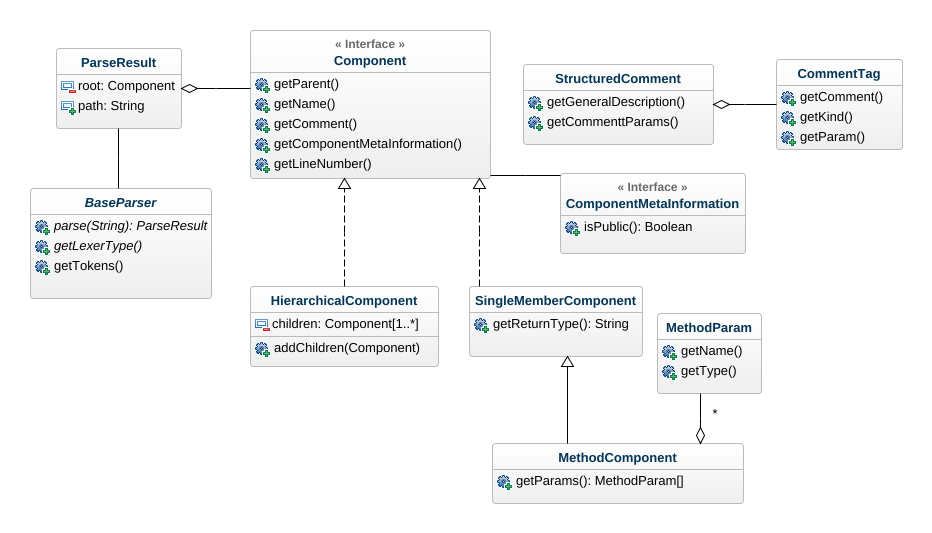
\includegraphics[height=9cm,keepaspectratio,angle=90]{figures/uml/parsing.png}
    \caption{UML-Diagramme aller Klassen, die relevant für das Parsen sind}
    \label{fig:uml_parsing}
\end{figure}
\chapter{UML-Diagramm: Metriken}\label{appendix_metrics_uml}
\begin{figure}[ht!]
\fontsize{5}{10}\selectfont
    \centering
    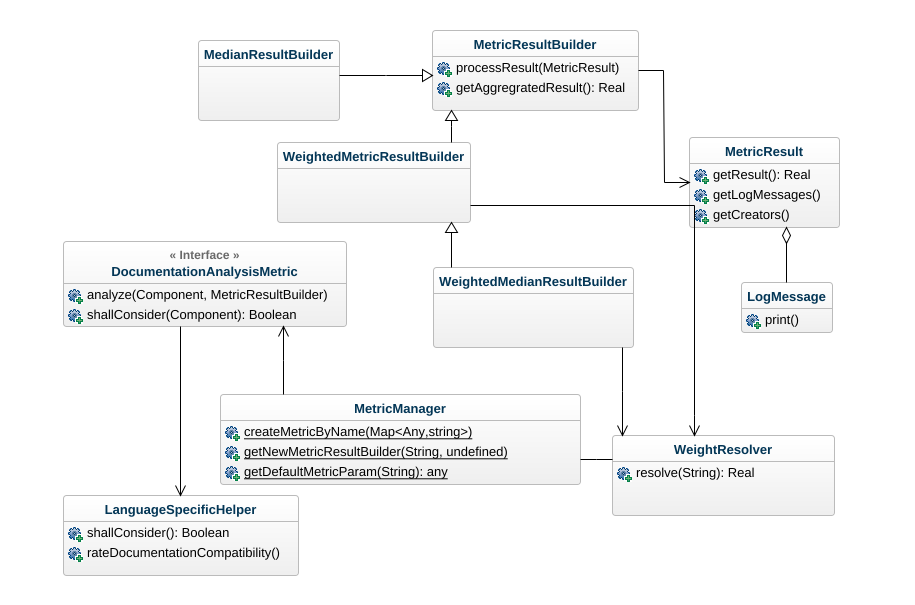
\includegraphics[height=10cm,keepaspectratio,angle=90]{figures/uml/metriken.png}
    \caption{UML-Diagramme aller Klassen, die relevant für die Metriken sind}
    \label{fig:uml_metrics}
\end{figure}
\chapter{Konfiguration des Tools}
\begin{description}
        \item[include]  Alle Dateien, die bei der Bewertung der Dokumentationsqualität berücksichtigt werden müssen
        \item[exclude]  Teilmenge von include, enthält Dateien, die nicht weiter betrachtet werden müssen
        \item[metrics]  Alle Metriken, die das Tool verwenden soll. Dies ist ein Array von Objekten mit der Struktur \enquote{(name,weight, unique\_name, params)}, wobei \textit{weight} das Gewicht der jeweiligen Metrik ist (Bei Algorithmen ohne Relevanz des Gewichts wird es ignoriert), \textit{name} der Name der Metrik und \textit{params} ein Objekt mit den Parametern der Metrik
        \item[absolute\_threshold] Mindestwert der Bewertung, die erreicht werden muss, sonst wird die Dokumentationsqualität nicht akzeptiert
       
          \item[builder] Der Algorithmus/\textit{ResultBuilder}, der die einzelnen Ergebnisse verarbeitet.
        
        \item[parser]  Kann verwendet, um die zu parsende Programmiersprache zu wählen. Dazu muss \textit{ParserFactory} angepasst werden
        
        \item[path\_weights] Ein Array von Objekten der Struktur \enquote{(path,weight)}. Wird verwendet, um einzelne Pfade höher oder niedriger zu gewichtet
        
         \item[component\_weights] Ein Array von Objekten der Struktur \enquote{(name,weight)}. Wird verwendet, um einzelne Komponenten höher oder niedriger zu gewichtet
         
         \item[default\_path\_weight] Das Standardgewicht für eine Datei, wenn keine passende Gewichtung gefunden wurde
         
         \item[default\_component\_weight] Das Standardgewicht einer Komponente, wenn keine passende Gewichtung gefunden wurde
         
         \item[state\_manager] Kann verwendet werden, um festzulegen, wie das letzte Ergebnis der Dokumentationsqualität gespeichert werden soll. Weitere Möglichkeiten können durch Erweiterung der \textit{StateManagerFactory} hinzugefügt werden.
         
         \item[relative\_threshold] Der maximale  relative Abstand zur letzten Dokumentationsqualität bevor eine Fehlermeldung geworfen wird.
         \item[builder\_params] Parameter für die \textit{MetricResultBuilder}. Diese wird aktuell nur von dem Squale-Builder (Kapitel \ref{chapter:squale}) genutzt
        
        
        
    \label{enum:tool_javadoc_conf}
\end{description}
\chapter{Implementierte Metriken}\label{appendix_metrics}

\begin{description}

\item[Anteil dokumentierter Komponenten an allen Komponenten]
\begin{description}
\item[]
    \item [Metrikname]  simple\_comment
    \item [Klassenname] SimpleCommentPresentMetric
    \item[Beschreibung] Berechnet den Anteil der dokumentierten Komponenten an allen Komponenten, kann Getter und Setter ignorieren
    \item[Quellen] \cite[S. 5]{HowDocumentationEvolvesoverTime}
\end{description}

\item[Anteil öffentlicher dokumentierter Komponenten]
\begin{description}
\item[]
    \item [Metrikname]  public\_members\_only
    \item [Klassenname] SimplePublicMembersOnlyMetric
    \item[Beschreibung] Berechnet den Anteil der öffentlichen dokumentierten Komponenten an allen öffentlichen Komponenten, kann Getter und Setter ignorieren
     \item[Quellen] \cite[S. 253]{JavadocViolationsandTheirEvolutioninOpen-SourceSoftware}
\end{description}

\item[Bestrafung langer undokumentierter Methoden]
\begin{description}
\item[]
    \item [Metrikname]  large\_method\_commented
    \item [Klassenname] SimpleLargeMethodCommentedMetric
    \item[Beschreibung] Bestraft undokumentierte Methoden je nach ihrer Länge
    \item[Quellen] Eigene Idee
\end{description}

\item[Vollständigkeit der Dokumentation von Methoden]
\begin{description}
\item[]
    \item [Metrikname]  method\_fully\_documented
    \item [Klassenname] SimpleMethodDocumentationMetric
    \item[Beschreibung] Prüft, ob alle Methodenparameter und Rückgabewert dokumentiert sind
    \item[Quellen] \cite[S. 5]{HowDocumentationEvolvesoverTime}
\end{description}
\clearpage
\item[Anteil dokumentierter Methoden unter
Berücksichtigung der LOC]
\begin{description}
\item[]
    \item [Metrikname]  commented\_lines
    \item [Klassenname] CommentedLinesRatioMetric
    \item[Beschreibung]  Berechnet den Anteil der \ac{LOC} der dokumentierten Methoden an allen \ac{LOC} aller Methoden
    \item[Quellen] Eigene Idee
\end{description}

\item[Flesch-Score]
\begin{description}
\item[]
    \item [Metrikname]  flesch
    \item [Klassenname] FleschMetric
    \item[Beschreibung]   Berechnet den Flesch-Score des Kommentars und bewertet so, ob der Kommentar verständlich ist
    \item[Quellen] \cite[S. 72]{AutomaticQualityAssessmentofSourceCodeComments:TheJavadocMiner}
\end{description}

\item[Kohärenz zwischen Kommentar und
Komponentenname]
\begin{description}
\item[]
    \item [Metrikname]  comment\_name\_coherence
    \item [Klassenname] CommentNameCoherenceMetric
    \item[Beschreibung]  Prüft, ob der Kommentar und der Name der dokumentierten Komponente sehr ähnlich sind oder keine Ähnlichkeit haben, arbeitet nur mit Methoden
    \item[Quellen] \cite[S. 86ff ]{Qualityanalysisofsourcecodecomments}
\end{description}

\item[Verwendung bestimmter Wörter bestrafen]
\begin{description}
\item[]
    \item [Metrikname]  certain\_terms
    \item [Klassenname] CertainTermCountMetric
    \item[Beschreibung]  Bestraft das Vorkommen bestimmter Wörter (wie z.~B. Abkürzungen)
     \item[Quellen] Inspiriert von Verbot lateinischer Ausdrücke nach \cite{HowtoWriteDocCommentsfortheJavadocTool}
\end{description}

\item[Bewertung der Formatierung]
\begin{description}
\item[]
    \item [Metrikname]  formatting\_good
    \item [Klassenname] FormattingGoodMetric
    \item[Beschreibung] Überprüft, ob korrekte Tags verwendet wurde, HTML-Tags geschlossen wurden und bei langen Methoden überhaupt eine Formatierung verwendet wurden
     \item[Quellen] Inspiriert von Regel in Checkstyle \cite{checkstyle_doc_metrics}
\end{description}

\clearpage
\item[Rechtschreibfehler bestrafen] 

\begin{description}
\item[]
    \item [Metrikname]  spellling
    \item [Klassenname] SpellingMetric
    \item[Beschreibung]Sucht nach Rechtschreibfehlern und bestraft sie
    \item[Quellen] Eigene Idee
\end{description}

\item[Erwähnung von Randfällen bei Methodenparameter
und -rückgabewerte]
\begin{description}
\item[]
    \item [Metrikname]  edge\_case
    \item [Klassenname] EdgeCaseMetric
    \item[Beschreibung] Prüft, ob bei der Dokumentation von Parametern die Behandlung des Wertes \textit{null} erwähnt wird
       \item[Quellen] Inspiriert von Idee in  \cite{javadoc_coding_standards}. In \cite[S.~1ff.]{@tComment:TestingJavadocCommentstoDetectComment-CodeInconsistencies} wird ebenfalls auf einer ähnlichen Art und Weise die Erwähnung von Randfällen geprüft, dort aber auch, ob diese Angaben korrekt sind
\end{description}


\item[Gunning-Fog-Index]
\begin{description}
\item[]
    \item [Metrikname]  gunning\_fog
    \item [Klassenname] GunningFogMetric
    \item[Beschreibung] Berechnet den Gunning-Fog-Index des Kommentars und bewertet so, ob der Kommentar verständlich ist
     \item[Quellen] \cite[S. 71]{AutomaticQualityAssessmentofSourceCodeComments:TheJavadocMiner}
\end{description}
 \end{description}

\chapter{Bilder des Tools}\label{chapter:pictures_tool}
In diesem Kapitel sind zwei Bilder des \textit{DoxEvaluators} abgedruckt, welche die zwei möglichen Ausgaben des Programms zeigen (Dokumentationsqualität ausreichend und nicht ausreichend):
\begin{figure}[htbp!]
    \centering
    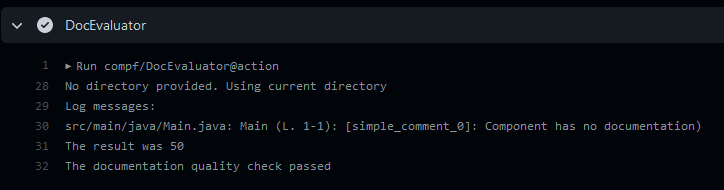
\includegraphics[width=\columnwidth]{figures/appendix/passed.png}
    \caption{Foto vom Tool: Dokumentationsqualität ausreichend}
    \label{fig:passed}
\end{figure}
\begin{figure}[htbp!]
    \centering
    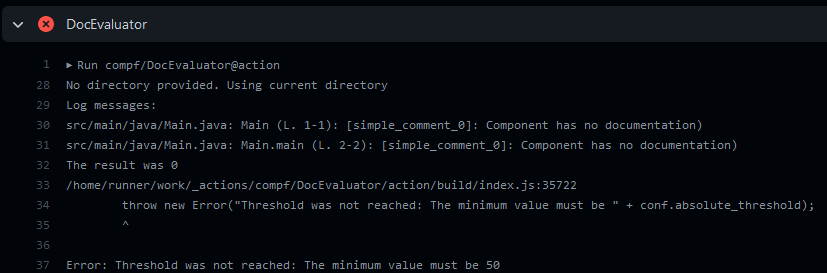
\includegraphics[width=\columnwidth]{figures/appendix/absolute_threshold.png}
    \caption{Foto vom Tool: Dokumentationsqualität zu schlecht}
    \label{fig:absolute}
\end{figure}

\end{appendices}
	


\clearpage
\chapter*{Erklärung zur selbstständigen Abfassung der Bachelorarbeit}

Ich versichere, dass ich die eingereichte Bachelorarbeit selbstständig und ohne unerlaubte Hilfe verfasst habe. Anderer als der von mir angegebenen Hilfsmittel und Schriften habe ich mich nicht bedient. Alle wörtlich oder sinngemäß den Schriften anderer Autoren entnommenen Stellen habe ich kenntlich gemacht. \\


\bigskip
\bigskip
\bigskip
\bigskip
\noindent
Osnabrück \today\\

\bigskip
\bigskip
\bigskip
\bigskip
\noindent
Timo Schoemaker
\end{document}





\clearpage
\chapter{Evaluation}\label{chapter:eval}
	\newcommand{\checkpmd}{\textit{Checkstyle} und \textit{PMD} }
\newcommand{\doceval}{\textit{DocEvaluator} }
In diesem Kapitel soll das Programm evaluiert werden, um zu prüfen, ob der \doceval eine gute heuristische Aussage über den Stand der Dokumentationsqualität treffen kann und in der Praxis auch einsetzbar ist. Dazu wird der \textit{DocEvaluator} mit \textit{Checkstyle} und \textit{PMD} verglichen, indem drei exemplarische Open-Source-Projekte mit allen drei Programmen analysiert werden und die Treffergenauigkeit und Geschwindigkeit der Programme verglichen werden. Zunächst müssen diese drei Projekte ausgewählt werden, was in Kapitel \ref{chapter:choosing_project} erläutert wird. Anschließend wird in Kapitel \ref{chapter:quality} beschrieben, wie die Evaluation der Treffergenauigkeit durchgeführt wird. In Kapitel \ref{chapter:speed} wird die Geschwindigkeitsevaluation durchgeführt. Zum Abschluss der Evaluation werden die Ergebnisse der Evaluation in Kapitel \ref{chapter:eval_conclusion} resümiert. 

\clearpage

\section{Wahl der zu analysierenden Projekte}\label{chapter:choosing_project}
Zur Durchführung der Evaluation wurden verschiedene Softwareprojekte aus GitHub heruntergeladen. Grundsätzlich kann der Vergleich mit jedem Java-Projekt durchgeführt werden, dennoch wurden einige Bedingungen festgelegt, die bei der Auswahl der Projekte eine wichtige Rolle spielen. Diese Bedingungen werden in der folgenden Auflistung präsentiert:

\begin{enumerate}
    \item \label{enum:size} Die Projekte müssen mindestens einen Umfang von 10~000 \ac{LOC} haben
    \item \label{enum:already_cited} Die Projekte müssen bereits in einer in dieser Bachelorarbeit zitierten Quelle in puncto Dokumentationsqualität analysiert worden sein
    \item \label{enum:parsing_error}  Die Projekte sollen möglichst wenige Parsing-Fehler beim \doceval produzieren. Bei mehr als zwei Fehlern wird ein Projekt nicht betrachtet. Können jedoch Fehler folgenlos behoben werden, so kann das Projekt dennoch betrachtet werden
    \item Das größte Projekt sollte mindestens zehnmal so groß sein wie das kleinste Projekt
\end{enumerate}

Die \ac{LOC} sollen nur als sehr grobe Heuristik der Größe eines Softwareprojektes verstanden werden und enthalten nur den reinen Code ohne Kommentare. Dabei wird heuristisch vermutet, dass mit steigender \ac{LOC} die Anzahl der Komponenten in einem Softwareprojekt steigt, wobei all diese Komponenten fehlerhaft (oder gar nicht) dokumentiert sein können. Somit dienen die \ac{LOC} als approximative Schätzung der zu erwartenden Fehler. 

 Durch die Bedingung in Nr. \ref{enum:size} wird sichergestellt, dass eine ausreichende Anzahl an Fehlern in der Dokumentation zu erwarten ist, um eine gute Analyse der Dokumentationsqualität  und eine aussagekräftige Bewertung der Geschwindigkeit zu ermöglichen. Durch die Bedingung in Nr.  \ref{enum:already_cited} werden nur Projekte in Betracht gezogen, die bereits in der wissenschaftlichen Literatur berücksichtigt wurden und daher (zumindest für den jeweiligen Autor der Quelle) geeignet für eine Analyse der Dokumentation sind. Mit der Bedingung in Nr. \ref{enum:parsing_error} wird eine Verzerrung zugunsten oder zuungunsten des \textit{DocEvaluators} vermieden, denn durch Parsing-Fehler können Komponenten falsch analysiert werden, die von den anderen Tools richtig analysiert werden. Indirekt wird dadurch gefordert, dass ein Projekt keine neueren Java-Funktionen verwendet, da  der \textit{DocEvaluator} nur Java bis Version 8 unterstützt. Die letzte Bedingung ist besonders für die Bewertung der Geschwindigkeit relevant, da so geprüft werden kann, ob der \doceval auch bei größeren Projekten noch in annehmbarer Zeit ein Ergebnis berechnen kann. 
 
 \subsubsection{Analysierte Projekte}\label{chapter:eval_projects}
 Die folgende Auflistung zeigt die gewählten Projekte für die Evaluation. Die Quellen verweisen auf das Verzeichnis in GitHub, das von den drei Tools analysiert werden soll.  In runden Klammern dahinter befinden sich die  (auf Zehntausenderstelle gerundeten) \ac{LOC}. 
 \begin{itemize}
  \item Log4J Version 1 \cite{log4j} (20~000)
    \item ArgoUML \cite{argouml} (17~000) 
     \item Eclipse \ac{JDT} \cite{eclipsejdt} (400~000)
 \end{itemize}
 
 ArgoUML und Eclipse wurden in \cite[S.~74] {AutomaticQualityAssessmentofSourceCodeComments:TheJavadocMiner} bewertet, wobei hier nur Eclipse \ac{JDT} betrachtet werden soll, da das gesamte Eclipse-Projekt zu umfassend ist. Log4J wurde in \cite[S.~267] {@tComment:TestingJavadocCommentstoDetectComment-CodeInconsistencies} betrachtet. 

 Bei allen Projekten traten zunächst Parsing-Fehler auf. Dies lag allerdings in den meisten Fällen daran, dass auskommentierte Methoden noch ein Javadoc-Präfix hatten. Dies kann vom \doceval nicht korrekt verarbeitet werden. Da diese Methoden offensichtlich nicht verwendet werden und keinen Einfluss auf die Qualität der Dokumentation haben können, wurden sie ersatzlos entfernt. Bei einem Fehler in Eclipse \ac{JDT} konnte der \doceval eine Datei mit mehr als 3000 Codezeilen nicht verarbeiten. Diese Datei wurde bei der Evaluation von allen Programmen ignoriert.

\section{Analyse der Qualität}\label{chapter:quality}
Durch die Evaluation der Qualität soll geprüft werden, ob der \doceval trotz des in Kapitel \ref{chapter_conception}
 beschriebenen abstrakten Formates eine Java-Datei richtig parsen kann und alle für die Dokumentation relevanten Informationen korrekt extrahieren kann. Zur Durchführung der Evaluation muss zunächst definiert werden, welche Funktionen der einzelnen Programme miteinander verglichen werden können, da die Programme unterschiedliche Aspekte der Dokumentation überprüfen und die Darstellung der Ergebnisse im Vergleich zum \textit{DocEvaluator} abweicht.

\checkpmd können als fehlersuchend bezeichnet werden. Sie prüfen die einzelnen Komponenten eines Programms und finden Abweichungen von vorher definierten Regeln. Eine solche Regel kann beispielsweise sein, dass jede öffentliche Methode dokumentiert sein muss, dass bestimmte Wörter nicht verwendet werden dürfen oder dass die Syntax der Dokumentation gültig sein muss. Damit sind sie vergleichbar mit den Metriken aus den Kapiteln \ref{chapter:metrics_coverage}  und \ref{chapter:metrics_errors}, welche ebenfalls bestimmte Fehler suchen und bei einem Verstoß gegen die Regeln eine Warnmeldung ausgeben. Allerdings berechnen \checkpmd keine Metriken, sondern finden nur die besagten Verstöße gegen die definierten Regeln. Somit kann ein Entwickler sehen, dasś ein Projekt beispielsweise 100 Verstöße gegen die Dokumentationsrichtlinien hat, erfährt aber nicht, ob die Anzahl der Verstöße unter Berücksichtigung der Projektgröße schwerwiegend ist und erhält keine normierte Bewertung, die dem Entwickler bei der Beurteilung der Dokumentationsqualität hilft. 

Im Gegensatz dazu verwendet der \doceval Metriken, die stets einen Wert von 0 bis 100 zurückgeben, sodass ein Entwickler weiß, dass ein hoher Wert für eine hohe Qualität steht. Außerdem kann der \doceval auch die Semantik des Kommentars heuristisch prüfen, um zu erfahren, ob der Kommentar verständlich ist und nicht redundant ist (vgl. Kapitel \ref{chapter:metrics_semantic}). Nichtsdestotrotz gibt der \doceval auch Warnmeldungen aus, wenn er bestimmte Komponenten schlechter bewerten muss.

Aus diesen Gründen wird die Evaluation nicht mit den Metriken an sich, sondern mit den Warnmeldungen der jeweiligen Tools durchgeführt. Jedes Programm wird mit einem Verweis auf das zu analysierende Projekt aufgerufen und die Ausgaben der Programme werden in separaten Dateien umgeleitet.  Diese Dateien dienen dann als Grundlage für die spätere Evaluation. 

\subsubsection{Durchführung der Evaluation}
Wie im vorherigen Absatz beschrieben, dienen die Logdateien der drei Programme als Datengrundlage für die Evaluation. Jede Zeile in diesen Logdateien enthält mindestens den Dateipfad des gefundenen Fehlers, die Zeilennummer des Fehlers und einen Fehlercode als Zeichenkette.  Wenn die drei Programme einen übereinstimmenden Fehler finden, sollte es in allen drei Logdateien einen Eintrag geben, bei dem der Dateipfad identisch ist, die Zeilennummer innerhalb eines gewissen Intervalls identisch ist und die der Fehlercode identisch ist. Die Zeilennummer muss nicht zwingend identisch sein, da  \checkpmd die exakte Zeile des Fehlers ausgeben, während der \doceval nur ein Intervall ausgibt, in dem der Fehler liegt. Beispielsweise wird von \checkpmd bei einem unzulässigen Wort die exakte Zeile des Wortes genannt. Da die drei Tools unterschiedliche Fehlercodes ausgeben, werden diese so kategorisiert, dass Verstöße, welche von mehr als einem Tool erkannt werden, einen eigenen Fehlercode erhalten. Alle anderen Verstöße erhalten einen allgemeinen programmspezifischen Fehlercode, der somit keine näheren Informationen über die Art des Fehlers hergibt.

Basierend auf diesen Vorbereitungen kann nun für jeden Fehler jedes Programm gefunden werden, das diesen Fehler entdeckt hat. Beispielsweise kann ein Fehler von allen drei Programmen, nur von \textit{Checkstyle} oder ausschließlich von \textit{PMD} und \doceval gefunden werden. Mathematisch gesehen kann die Potenzmenge der Menge \textit{\{Checkstyle, PMD, DocEvaluator\}} genommen werden, wodurch alle möglichen Kombinationen an Programmen entstehen, die einen bestimmten Fehler erkennen können. Durch Zählen der Fehler pro Programmkombination lässt sich bewerten, welche Programme besonders viele Fehler finden, die andere Programme nicht erkennen und ob alle drei Programme viele gemeinsame Fehler finden. 


\subsubsection{Auswahl der Regeln}
Zum Vergleich der drei Programme müssen zunächst Regeln festgelegt werden, bei denen die Programme eine Warnmeldung ausgeben. Bei \checkpmd{} erfolgt die Konfiguration über  Extensible-Markup-Language-Dateien. Beim \doceval erfolgt die Konfiguration über das in Kapitel \ref{chapter:conf} beschriebene \ac{JSON}-Format. Bei der Auswahl der Regeln muss beachtet werden, dass \checkpmd auch andere Fehler wie z.~B. komplexe Methoden finden können. Diese sind in diesem Kontext nicht relevant und werden ignoriert. Außerdem können die drei Programme zum Teil unterschiedliche Fehler finden, da beispielsweise \textit{PMD} (anders als \textit{Checkstyle}) den Inhalt der Dokumentation auf das Auftauchen bestimmter Begriffe prüfen kann.  \textit{Checkstyle} kann aber dafür (anders als \textit{PMD}) prüfen, ob die Block-Tags in der richtigen Reihenfolge definiert werden. Die letztere Regel wird vom \doceval in der ausgelieferten Fassung nicht geprüft. Alle drei Programme können jedoch prüfen, ob eine Komponente dokumentiert ist oder nicht. Tabelle \ref{tab:inters_rules} vergleicht die Überschneidungen der Regeln, welche die drei Programme anwenden können. Dabei stehen (sowohl hier als auch im Rest des Kapitels 5) die Abkürzungen \textit{CS} für \textit{Checkstyle} und \textit{DE} für \textit{DocEvaluator}.

\begin{table}[]
    \centering
    \begin{tabular}{m{4.5cm}|m{4.5cm}|m{4.5cm}}
     \textbf{CS} $\cap$ \textbf{DE}  & \textbf{PMD} $\cap$ \textbf{DE} & \textbf{PMD} $\cap$ \textbf{DE} $\cap$  \textbf{CS}  \\\hline
     \begin{itemize}
        \item Komponente dokumentiert
        \item Methode vollständig dokumentiert
         \item Fehler in Javadoc
     \end{itemize}
      & 
      \begin{itemize}
          \item  Komponente dokumentiert

          \item Bestimmte Wörter in Kommentar verbieten
      \end{itemize}
      & 
       \begin{itemize}
          \item  Komponente dokumentiert
         
      \end{itemize}
      \\\hline
    \end{tabular}
    \caption{Überschneidungen der Regeln der drei Programme}
    \label{tab:inters_rules}
\end{table}

Aus der Tabelle lässt sich entnehmen, dass der \doceval mit \textit{Checkstyle} die meisten Übereinstimmungen hat. Beide Programme können die Vollständigkeit der Methodendokumentation und typische Fehler in Javadoc-Kommentaren (wie z.~B. fehlerhaftes HTML) finden. PMD und der \doceval können bestimmte Wörter in der Dokumentation bemängeln, die in einer Dokumentation vermieden werden sollten. Alle drei Programme können das Vorhandensein der Dokumentation überprüfen. Allerdings ignoriert \textit{PMD} alle privaten Komponenten außer Felder. Vor allem bei Checkstyle gibt es zudem viele Regeln, die von den anderen beiden Programmen nicht gefunden werden und auf der Webseite \cite{checkstyle_doc_metrics} aufgelistet werden.

Da ein Vergleich der drei Tools somit nur eingeschränkt möglich ist, wird sich die qualitative Evaluation nur auf den Kernbereich beschränken. Es werden also nur die Regeln verwendet, die von mindestens zwei Tools unterstützt werden. Dies sind alle Regeln in Tabelle \ref{tab:inters_rules}. Da somit nur relativ leichte Fehler gefunden werden, können die Ergebnisse der Evaluation dazu verwendet werden, um die Parsing-Qualität zu ermitteln, denn wenn solche grundlegenden Fehler (wie z.~B. das Nichtvorhandensein der Dokumentation) nicht gefunden werden, besteht eine erhebliche Chance, dass eine Java-Datei falsch interpretiert wird. 



\subsection{Ergebnisse}

Tabelle \ref{tab:eval_results} listet die Anzahl der gefundenen Fehler (gemäß Tabelle \ref{tab:inters_rules}) auf. In den Spalten werden die Fehler nach dem Projekt gruppiert. Die ersten drei Zeilen beschreiben, wie viele Fehler die einzelnen Tools pro Projekt gefunden haben. So hat  der \textit{DocEvaluator} 1710 Fehler in \textit{Log4J} gefunden.  In den übrigen Zeilen wird aufgeführt, welche Kombinationen der Tools wie viele Fehler gefunden haben. Die Zeile mit der ersten Spalte \enquote{\{PMD, DE\}} beschreibt beispielsweise, dass \textit{PMD} und der  \textit{DocEvaluator} (aber nicht \textit{Checkstyle}) 41 Fehler bei \textit{Log4J}, 264 Fehler bei \textit{ArgoUML} und 253 Fehler bei \textit{Eclipse \ac{JDT}} gefunden haben. 
\sisetup{group-minimum-digits=4,table-number-alignment =center,table-format=5.0}
\begin{table}[]
    \centering
\begin{tabular}{c|S|S|S}
          & {Log4J} & {ArgoUML} & {Eclipse \ac{JDT}} \\ \hline
|DE|            & 1710 & 10054  & 17380      \\ \hline
|CS|            & 1590 & 9961   & 17638      \\ \hline
|PMD|           & 1008 & 9051   & 12702      \\ \hline\hline
\{DE\}          & 108   & 124     & 555         \\ \hline
\{CS\}          & 26    & 285     & 273         \\ \hline
\{PMD\}         & 86    & 377     & 298         \\ \hline
\{PMD, DE\}     & 41    & 264     & 253         \\ \hline
\{CS, DE\}      & 683   & 1266    & 5214       \\ \hline
\{PMD, CS\}     & 3     & 10      & 793         \\ \hline
\{PMD, CS, DE\} & 878   & 8400   & 11358      \\ \hline
\end{tabular}
    \caption{Anzahl der gefundenen Fehler pro Projekt}
    \label{tab:eval_results}
\end{table}

Aus der Tabelle ist ersichtlich, dass stets über 50~\% aller Fehler von allen drei Tools gefunden werden. Bei \textit{Eclipse \ac{JDT}} und \textit{Log4J} werden mehr als ein Viertel der Fehler von der Kombination  \textit{DocEvaluator} und \textit{Checkstyle} gefunden. Beim Projekt \enquote{ArgoUML} liegt diese Quote bei weniger als 15~\%.  Weniger als 10~\% der Fehler werden nur von einem Tool erkannt. 

Die Überschneidungen der Fehler lassen sich auch mit Venn-Diagrammen darstellen.  Die Abbildungen \ref{fig:log4j_venn}, \ref{fig:argo_venn} und  \ref{fig:eclipse_venn} zeigen für jedes Projekt die Überschneidungen der gefundenen Fehler. Die Abbildung \ref{fig:legend_venn} ist die Legende dieser drei Abbildungen:


\begin{figure}[ht!]
\centering
   \begin{subfigure}[b]{0.4\textwidth}
    \centering
\includesvg[scale=0.7,width=\textwidth]{figures/chapter5/log4j.svg}
    \caption{Venn-Diagramm: Log4J}
    \label{fig:log4j_venn}
\end{subfigure}
\hfill
\begin{subfigure}[b]{0.4\textwidth}
    \centering
\includesvg[scale=0.7,width=\textwidth]{figures/chapter5/argo.svg}
    \caption{Venn-Diagramm: ArgoUML}
    \label{fig:argo_venn}
\end{subfigure}
\hspace{10cm}
\begin{subfigure}[b]{0.4\textwidth}
    \centering
\includesvg[scale=0.7,width=\textwidth]{figures/chapter5/eclipse.svg}
    \caption{Venn-Diagramm: Eclipse \ac{JDT}}
    \label{fig:eclipse_venn}
\end{subfigure}
\hspace{3.4cm}
\begin{subfigure}[b]{0.25\textwidth}
    \centering
\includesvg[width=1\textwidth]{figures/chapter5/legende_venn.svg}
\vspace{0.3cm}
    \caption{Legende der Venn-Diagramme}
    \label{fig:legend_venn}
\end{subfigure}
\end{figure}

  Auch hier zeigt der graue Bereich visuell, dass die drei verglichenen Tools viele Fehler gemeinsam finden.  Dies ist vor allem bei \textit{ArgoUML} deutlich, da der graue Kreis fast alle anderen Kreise großflächig überdeckt. Bei den anderen beiden Projekten ist zudem eine große Überschneidung von \textit{Checkstyle} und \doceval (hellbraun) zu erkennen. Bei \textit{Log4J} zeigt das Diagramm einen im Vergleich zu den anderen Projekten größeren Bereich (dunkelblau) an Fehlern, die nur von \textit{PMD} gefunden werden. Auch der Bereich der exklusiv vom \textit{DocEvaluator} gefundenen Fehler (rot) ist bei \textit{Log4J} größer. Die nur vom \textit{DocEvaluator} und \textit{PMD} gefundenen Fehler (lila) sind bei  \textit{Eclipse \ac{JDT}} nicht zu erkennen, bei den anderen Venn-Diagrammen allerdings schon. Dafür scheint es bei  \textit{Eclipse \ac{JDT}} relativ viele Fehler zu geben, die nur von \checkpmd gefunden werden, da der hellblaue Abschnitt nur dort sichtbar ist. Außerdem gibt es bei  \textit{Eclipse \ac{JDT}} mehr Fehler, die nur von \textit{Checkstyle} gefunden werden, da der grüne Bereich größer ist. 

Um die Trefferrate mathematisch auszudrücken, kann die Formel
\begin{equation}\label{eq1}
    1-\frac{\text{\{DE\}}}{|\text{DE}|}
\end{equation} verwendet werden. Diese gibt in Prozent an, wie viele Fehler, die vom \doceval gefunden werden, auch von den anderen beiden Tools gefunden werden. Demgegenüber kann auch ermittelt werden, wie viele Fehler von \textit{Checkstyle} oder \textit{PMD} gefunden wurden, die auch vom \doceval erkannt wurden:

\begin{equation}\label{eq2}
    1-\frac{\text{\{CS\}}+\text{\{PMD\}}+\text{\{CS,PMD\}}}{|\text{PMD}|+|\text{CS}|}
\end{equation}

Tabelle \ref{tab:hit_rate} zeigt basierend auf den genannten Formeln (\ref{eq1} und \ref{eq2}) die Treffergenauigkeit des \textit{DocEvaluators} für jedes analysierte Projekt:
\begin{table}[]
    \centering
    \begin{tabular}{c|c|c|c}
    Formel & Log4J & ArgoUML & Eclipse \ac{JDT} \\ \hline
    \ref{eq1} &   93,68~\% &	98,77~\% &	96,81~\% \\\hline
     \ref{eq2} & 95,57~\% &	96,47~\% &	95,50~\% \\\hline

    \end{tabular}
    \caption{Trefferrate des \textit{DocEvaluators} gemäß den Formeln \ref{eq1} und \ref{eq2}}
    \label{tab:hit_rate}
\end{table}
Es ist klar erkennbar, dass die Trefferrate unabhängig von der Formel und dem analysierten Projekt größer als 90~\% ist, sodass die meisten Fehler, die vom \doceval gefunden werden, von mindestens einem anderen Tool gefunden werden. Zudem werden die meisten Fehler, die von \textit{Checkstyle} oder \textit{PMD} gefunden werden, auch vom \doceval gefunden.






\subsection{Bewertung der Qualitätsevaluation}
Insgesamt zeigt die Evaluation der Qualität, dass der \doceval eine hohe Abdeckung mit \checkpmd hat und somit die meisten von diesen Tools gefundenen Fehler auch findet. Somit ist das abstrakte Format zur Repräsentation einer Quellcodedatei geeignet, um die meisten Aspekte, welche für die Dokumentation relevant sind, zu beschreiben. Allerdings wurde diese Evaluation auf größere Projekte (über 10~000 \ac{LOC}) beschränkt, sodass nicht geprüft wurde, ob der \doceval auch bei kleineren Projekten eine genaue Einschätzung der Dokumentationsqualität gibt. Tendenziell wird die Trefferrate kleiner sein, da durch die geringere Größe jeder nicht gefundene Fehler ein höheres Gewicht hat. 

Während der Evaluation wurde geprüft, warum einige Fehler nicht vom \doceval gefunden wurden. In einigen Fällen waren dies einfache Fehler, die bereits behoben sind, sodass dadurch die Trefferrate erhöht wurde. In anderen Fällen gibt es größere strukturelle Probleme, die nicht mehr leicht behebbar sind. Einige dieser Fehler werden im Folgenden präsentiert: 
\subsubsection{Fehler durch verschiedene Zeilennummerierung}

Einige Fehler sind keine Fehler des \textit{DocEvaluators} an sich, sondern sind in der Methodik der Evaluation begründet. Um gemeinsame Fehler zu finden, müssen die gefundene Fehler pro Tool abgeglichen werden, wozu die Zeilennummer elementar ist. Allerdings gibt es Unterschiede bei der Festlegung der Zeilennummer. Der \doceval verwendet in seiner Logausgabe ein Zeilennummerintervall, der mit der Zeile des Bezeichners der Komponente endet und dessen Anfang durch Subtraktion der Anzahl der Zeilen der Dokumentation von der Zeile des Bezeichners definiert wird. Die anderen Tools verwenden die exakte Zeile eines Fehlers. In den meisten Fällen ist dies kein Problem, da diese Zeilennummer von \checkpmd innerhalb des vom \doceval beschriebenen Intervalls liegen muss. Listing \ref{lst:multiline_method} zeigt ein Beispiel, wo es problematisch wird.

		\begin{figure}[ht!]
			\lstinputlisting
			[caption={Methode auf viele Zeilen verteilt},
			label={lst:multiline_method},
			captionpos=b,language=java, basicstyle=\footnotesize, tabsize=1, showstringspaces=false,  numbers=left]
			{figures/chapter5/multiline_method.java}
		\end{figure}
Besonders an dieser Methode ist, dass die Parameter auf verschiedenen Zeilen verteilt ist. Während \textit{Checkstyle} bei einem undokumentierten Parameter die exakte Zeile eines nicht dokumentierten Parameters ausgibt (z.~B. Z. 5), würde der \doceval die Zeilen 1 bis 4 ausgeben, da die Dokumentation bei Zeile 1 beginnt und der Bezeichner der Komponente in Zeile 4 definiert ist. Ähnlich problematisch ist es, wenn zwischen der Dokumentation und dem Bezeichner noch Annotationen stehen, sodass der Bezeichner um eine Zeile nach unten rutscht.  

\subsubsection{Klassen in Methoden}

In Java können Klassen in Methoden deklariert werden bzw. anonyme Klassen direkt instantiiert werden. Diese Klassen können ebenfalls Javadoc besitzen, werden allerdings vom \doceval ignoriert, da der \doceval jeglichen Code in Methoden nur unstrukturiert als Zeichenkette speichert und nicht weiterverarbeitet. Die anderen beiden Tools prüfen auch diese Klassen, sodass sie entsprechend einige Fehler finden, die der \doceval nicht mehr finden kann. 


\subsubsection{Fehler in einzeiligen Kommentaren bei PMD}
Anders als der \doceval und \textit{Checkstyle} berücksichtigt \textit{PMD} auch einzeilige Kommentare. Wenn ein einzeiliger Kommentar ein unzulässiges Wort enthält, so würde \textit{PMD} einen Fehler melden, aber der \doceval nicht, da er nur Javadoc-Kommentare prüft. Dadurch kommt es zu einer Verzerrung und der Anteil der alleinig von \textit{PMD} gefundenen Fehler wird überschätzt.  



 \section{Analyse der Geschwindigkeit} \label{chapter:speed}
 In diesem Abschnitt wird der \doceval mit \checkpmd bezüglich der Geschwindigkeit verglichen. Damit soll geprüft werden, ob das Tool nicht nur eine ausreichende Qualität besitzt, sondern auch in einer angemessenen Zeit ein Ergebnis liefert. Dies ist im \ac{CI/CD}-Kontext wichtig, da bei einer langen Laufzeit des Tools  die Bereitstellung eines geprüften Softwareprojektes verzögert wird und somit die Produktivität reduziert wird. 
 
 \subsubsection{Durchführung der Geschwindigkeitsevaluation}
 Zur Durchführung der Evaluation der Geschwindigkeit analysieren die drei Tools die in Kapitel \ref{chapter:eval_projects} genannten Projekte. Damit jedes Programm fair behandelt wird und eine ungefähr gleiche Menge an Analysen durchführen kann, werden die Regeln so beschränkt, dass nur noch das Vorhandensein von Dokumentation geprüft wird. So wird verhindert, dass beispielsweise der \textit{DocEvaluator} und \textit{Checkstyle} die Dokumentation von Methodenparameter überprüfen, während \textit{PMD} dies ignoriert. Bei jeder Analyse wird die Zeit gemessen, die vom Start eines Tools bis zu dessen Beendigung vergehen. 
 
 Die Ausgabe jedes Tools wird auf \enquote{dev/null} umgeleitet, sodass jegliche Ausgabe ignoriert wird. Dadurch können Schwankungen unberücksichtigt bleiben, die bei der Verwendung von Eingabe- und Ausgabegeräten auftreten. So sind die Ergebnisse näher an der tatsächlichen Verarbeitungsgeschwindigkeit.  Nachteilhaft an diesem Vorgehen ist, dass die Tools im Praxiseinsatz eine Ausgabe produzieren müssen, um überhaupt dem Entwickler helfen zu können, sodass dieser wichtige Aspekt hier ignoriert wird. 
 
 Die Analyse jedes Projektes mit jedem Tool wird zehnmal durchgeführt, um Schwankungen durch Hintergrundprozesse oder andere Einflussfaktoren auszugleichen. Die Evaluation der Geschwindigkeit wird auf einem Laptop mit dem Prozessor \enquote{i7-1165G7} mit 16 GB Arbeitsspeicher durchgeführt. Dabei wurden alle Programme auf dem Computer geschlossen und die Berechnungen wurden ohne grafische Benutzeroberfläche durchgeführt, um Schwankungen in der Laufzeit zu minimieren.  
 \subsection{Ergebnisse}\label{chapter:eval_speed_result}
 Die Tabellen \ref{tab:median_speed} und \ref{tab:std_speed} zeigen den Median und die Standardabweichung der benötigten Durchlaufzeit pro Tool und Projekt in Sekunden. Die Abbildungen \ref{fig:log4j_box}, \ref{fig:argo_box} und \ref{fig:eclipse_box} visualisieren den Inhalt der Tabellen als Boxplot. 
 
Im Verzeichnis \enquote{speed\_eval} des digitalen Anhangs befinden sich die Rohdaten der Geschwindigkeitsmessung, gruppiert nach dem analysierten Projekt. Auch die Originaldateien der Boxplots befinden sich dort. 
 \sisetup{group-minimum-digits=4,table-number-alignment =center,table-format=2.3,output-decimal-marker = {,}}
 \begin{table}[ht!]
     \centering
     \begin{tabular}{c|S|S|S}
        & {DE} & {CS} & {PMD}  \\\hline
        Log4J & 2.538 & 2.30 & 1.907\\\hline 
        ArgoUML & 16.965 & 9.301 & 7.917 \\\hline
        Eclipse \ac{JDT} & 69.148 & 27.316 & 21.586
     \end{tabular}
     \caption{Median der Laufzeit in Sekunden}
     \label{tab:median_speed}
 \end{table}
 
  \begin{table}[ht!]
     \centering
     \begin{tabular}{c|S|S|S}
        & {DE} & {CS} & {PMD}  \\\hline
        Log4J & 0,077 &  0,174 &  0,068\\\hline 
        ArgoUML & 0,197 &  0,083 & 0,157 \\\hline
        Eclipse \ac{JDT} & 1,594 & 0,265 & 0,270\\\hline
     \end{tabular}
     \caption{Standardabweichung der Laufzeit in Sekunden}
     \label{tab:std_speed}
 \end{table}
 
 \begin{figure}
 \centering
    \begin{subfigure}[b]{0.49\textwidth}
    \centering
\includesvg[width=\textwidth]{figures/chapter5/log4j_speed_boxplot.svg}
    \caption{Boxplot: Log4J}
    \label{fig:log4j_box}
\end{subfigure}
\hspace{0.01cm}
 \begin{subfigure}[b]{0.49\textwidth}
    \centering
\includesvg[width=\textwidth]{figures/chapter5/argo_speed_boxplot.svg}
    \caption{Boxplot: ArgoUML}
    \label{fig:argo_box}
\end{subfigure}

 \begin{subfigure}[b]{0.49\textwidth}
    \centering
\includesvg[,width=\textwidth]{figures/chapter5/eclipse_speed_boxplot.svg}
    \caption{Boxplot: Eclipse \ac{JDT} }
    \label{fig:eclipse_box}
\end{subfigure}
   
 \end{figure}
 

Aus den Tabellen und Boxplot-Diagrammen wird ersichtlich, dass der \doceval im Durchschnitt länger benötigt, um die Projekte zu bewerten. Wie aus dem Boxplot-Diagramm \ref{fig:log4j_box} zu entnehmen ist, gab es nur bei Log4J einen Ausreißer, bei dem \textit{Checkstyle} mehr Zeit benötigt hat.   Ansonsten war \textit{Checkstyle} stets schneller als der \textit{DocEvaluator}. \textit{PMD} analysiert am schnellsten ein Projekt. Der Unterschied in der Laufzeit zwischen dem \doceval und den anderen Tools steigt stark  mit wachsender Größe des analysierten Projektes.  Bei dem kleinsten Projekt \textit{Log4J} benötigt der \doceval  durchschnittlich die 1,103-fache Zeit im Vergleich zu \textit{Checkstyle}. Bei dem größten Projekt \textit{Eclipse \ac{JDT}} benötigt der \doceval durchschnittlich 2,53-mal so viel Zeit wie \textit{Checkstyle}. Beim \doceval und \textit{PMD} steigt die Standardabweichung mit der Größe des Projektes, während dieser Trend bei \textit{Checkstyle} nicht so eindeutig ist.

Bei dem Boxplot-Diagramm \ref{fig:log4j_box} zu \textit{Log4J} ist auch erkennbar, dass Ausreißer der Laufzeit nach oben häufiger sind als nach unten, da der Median sich stets im unteren Bereich des Boxplot-Quartils befindet. Bei den anderen Projekten ist dies aufgrund des größeren Zeitabstandes  zwischen dem \doceval und den anderen Tools  und der daraus resultierenden Verkleinerung der einzelnen Boxplots  nicht so klar im Boxplot ersichtlich, allerdings stimmt diese Aussage größtenteils auch dort. Nur bei der Analyse von \textit{ArgoUML} durch den \doceval (Abbildung \ref{fig:argo_box}) scheinen Abweichungen nach unten häufiger zu sein.

\subsection{Bewertung der Ergebnisse}
Insgesamt zeigt die Evaluation der Geschwindigkeit, dass der \doceval langsamer arbeitet als die anderen Programmen. Allerdings  bleibt die Laufzeit auf einem angemessenen Niveau, da die Verarbeitung von dem größten Projekt \textit{Eclipse \ac{JDT}} mit 400~000 \ac{LOC} im Durchschnitt nur etwas mehr als einer Minute benötigt. Nichtsdestotrotz ignoriert diese Analyse, dass die Ausgabe von Ergebnissen über die Konsole hier nicht berücksichtigt wurde und nur eine einfache Metrik angewendet wurde. Bei einem Experiment mit aktivierter Ausgabe wurden ähnliche Ergebnisse produziert, insbesondere ist der \doceval weiterhin das langsamste Programm. 

Für die schlechtere Laufzeit des \doceval im Vergleich zu \checkpmd lassen sich zwei Hauptargumente finden. So soll \textit{Node.Js}, welches die Plattform des Tools ist, langsamer sein als Java, in dem \checkpmd programmiert sind \cite{node_java_speed}.  Außerdem ist zu beachten, dass der \doceval Metriken berechnen soll und daher die Zwischenergebnisse aller Komponenten speichern muss, um daraus ein Gesamtergebnis mittels eines arithmetischen Mittelwerts oder eines anderen Algorithmus' berechnen zu können. Auch wenn dieses Gesamtergebnis bei der Laufzeitevaluation uninteressant ist, wird es dennoch berechnet, was zusätzliche Laufzeit benötigt. Dies erklärt auch die starke Steigerung des Zeitaufwands bei größeren Projekten.

\section{Fazit der Evaluation}\label{chapter:eval_conclusion}

Insgesamt zeigt die Evaluation sowohl bezüglich der Qualität als auch der Geschwindigkeit, dass der \doceval mit den anderen Tools mithalten kann. Zwar wird nicht jeder Fehler gefunden, aber die Trefferrate ist hoch und durch die Verwendung eines abstrakten Formates, das für mehrere Programmiersprachen geeignet ist, sind solche Abstriche nicht vermeidbar. 

Auch bei der Geschwindigkeit zeigt sich, dass der \doceval zwar im Extremfall zweieinhalbmal langsamer ist als die anderen Tools, allerdings ist die Laufzeit mit knapp 70 Sekunden im Extremfall bei einem großen Projekt noch in einem (relativ) angemessenen Rahmen. Nichtsdestotrotz ist es eine Überlegung wert, den \doceval weiter zu optimieren, damit die Laufzeit verbessert wird. 
\begingroup
\renewcommand{\cleardoublepage}{} % TODO maybe removing this and next
\renewcommand{\clearpage}{}
\chapter{Conclusion}\label{chapter:conclusion}
\endgroup
\label{sec:conclusion}
Ziel dieser Bachelorarbeit war es, ein Tool zu Bewertung der Dokumentation zu entwickeln, das in einem \ac{CI/CD}-Prozess eingebunden werden kann und nicht auf einer Programmiersprache beschränkt ist. Dabei beschränkt sich diese Bachelorarbeit auf strukturierte Kommentaren wie z.~B. Javadoc. Dieses Ziel wurde im Großen und Ganzen erreicht.

Durch die allgemein gehaltene Klassenstruktur für das Parsing ist es möglich, Quellcode in anderen Programmiersprachen bewerten zu lassen. Allerdings muss dafür ein entsprechender Parser geschrieben werden, welcher den Quellcode in die vorgegebene Struktur transformiert. Dabei ist es natürlich nicht möglich, jedes Detail abzubilden, sondern es müssen Abstriche gemacht werden. Nichtsdestotrotz können auch sprachspezifische Eigenheiten berücksichtigt werden, indem eine entsprechende abgeleitete Klasse von \textit{ComponentMetaInformation} gebildet wird und diese sprachspezifischen Informationen dort gespeichert werden. Diese Daten können von einem geeigneten \textit{LanguageSpecificHelper} dazu verwendet werden, um sprachabhängige Details bei der Bewertung der Dokumentation zu berücksichtigen. 

Auch das Parsen der strukturierten Kommentare erfolgt recht abstrakt, indem  die Informationen in den Beschreibungstexten unstrukturiert als Zeichenketten gespeichert werden, sodass die einzelnen Metriken diese Informationen weiterverarbeiten müssen. Da es Metriken gibt, die mit den einzelnen Wörtern ein eines Kommentars arbeiten und auch Metriken, welche die interne Struktur des Kommentars analysieren, wäre es ein mögliches Forschungsthema, wie diese zwei Darstellungen besser repräsentiert werden können. 

Um das Tool konfigurierbar zu halten, wurde ein Konzept für eine Konfigurationsdatei im \ac{JSON}-Format vorgestellt, das alle wichtigen Informationen enthält. Die Konfiguration kann auch über GitHub Actions durchgeführt werden, indem passende Umgebungsvariablen gesetzt werden.  So kann das Tool sowohl als reguläres Programm auf einem lokalen System verwendet werden als auch mittels GitHub Actions in den \ac{CI/CD}-Prozess eingebunden werden. Durch die flexible Konfiguration kann ein Nutzer frei entscheiden, welche Metriken er für sinnvoll hält und wie er sie gewichten will. Dabei überschreibt die Konfiguration mittels GitHub Actions stets die Konfiguration in der \ac{JSON}-Datei. Außerdem können die Metriken selbst begrenzt konfiguriert werden. Eine Nutzung des Tools auf anderen \ac{CI/CD}-Plattformen, die mit GitHub Actions vergleichbar sind,  ist prinzipiell ebenfalls möglich, da die Konfiguration von dem  übrigen Programm entkoppelt ist.

Für das Tool wurden bereits einige Metriken entwickelt, welche verschiedene Bereiche der Dokumentation analysieren können. Leider war eine Evaluation der einzelnen Metriken nicht möglich, sodass weiterhin offenbleibt, welche Metriken in welchen Situationen valide Ergebnisse liefern und wie eine sinnvolle Gewichtung der Metriken aussehen kann.  Weitere Metriken lassen sich durch Einfügen einer neuen abgeleiteten Klasse von \textit{DocumentationAnalysisMetric} bilden. Schwierig kann im konkreten Einzelfall allerdings das Finden einer geeigneten Funktion werden, welche die Werte der Metrik in das vorgegebene Intervall von 0 bis 100 transformiert. Mögliche Ideen für weitere Metriken lassen sich in \cite{checkstyle_doc_metrics} finden. Auch die wissenschaftliche Literatur liefert weitere Metriken, die fortschrittliche Techniken im Bereich des \ac{NLP} nutzen und daher im Rahmen dieser Bachelorarbeit zu komplex waren. Beispielhaft sei hier das Tool \enquote{iComment} aus  \cite[S.~145ff.]{icomment} genannt, bei dem geprüft wurde, ob die Dokumentation mit dem Code auch konsistent ist und somit korrekt und aktuell ist. Diese Metriken können als Inspiration genommen werden, um die Dokumentationsqualität umfassender analysieren zu können, sodass Entwickler bei der Identifikation und Behebung von mangelhafter Softwaredokumentation  besser unterstützt werden.





%Prints references
\printbibliography[title=Literature]


\clearpage 

%Appendix (comes after bibliography)

\renewcommand\appendixpagename{Anhänge}
\begin{appendices}


\chapter{Änderungen an der Parserdatei}\label{chapter:appendix_parser_changes}

\begin{table}[h!]
    \centering
    \begin{tabular}{m{0.75cm}|m{4cm}|m{10cm}}
        \textbf{Zeile} & \textbf{Änderung} & \textbf{Begründung} \\
         \hline
        116 & Deklaration Kommentar & Hier wird ein mehrzeiliger Kommentar definiert, dies ist hier ein Alias für den Token \textit{JCOMMENT}\\
        \hline
        127--128 & \textit{comment} als mögliches Präfix in Klassenmember & Hier wird dem Parser mitgeteilt, dass ein Bestandteil einer Klasse wie z. B. eine Methode einen Javadoc-Kommentar besitzen kann\\
        \hline
        47 & \textit{comment} als mögliches Präfix vor Datentyp & Hier wird dem Parser mitgeteilt, dass ein Datentyp (Klasse, Schnittstelle etc. ) einen Javadoc-Kommentar haben kann \\
        \hline
        404 & Zulassung von Javadoc in Methoden & Da Javadoc-Kommentare an beliebigen Stellen auftauchen können, auch wenn es nicht empfohlen wird und keinen Mehrwert bietet, wird hier sichergestellt, dass solche Kommentare nicht zu Warnungen oder Fehler von ANTLR4 führen. Diese Javadoc-Kommentare werden nichtsdestotrotz später ignoriert\\
        \hline
        34, 38& Zulassung von Kommentaren vor Paketdeklarationen und Imports & Hier werden Kommentare auch vor Paketdeklarationen und Import-Statements erlaubt, was vor allem bei Klassen mit Urheberrechtsangabe sinnvoll ist\\
        \hline
        105 & Zulassung von Kommentaren bei Enumerationen & Zwar werden Javadoc-Kommentare in Enumerationen mit diesem Tool nicht betrachtet, sie führen aber dennoch zu Warnungen und Fehlermeldungen. Daher werden sie hier zugelassen, aber später ignoriert \\
        \hline
        82, 83 & Erzeugung eines separaten Knotens für \textit{Extends}- und \textit{Implements}-Deklarationen & In der originalen Version der Parserdatei wurde die Definition der Basisklasse bzw. der implementierten Schnittstellen direkt über die Tokens \textit{EXTENDS} bzw. \textit{IMPLEMENTS} gelöst. Dies wurde in einem neuen Knoten \textit{extendClass} bzw. \textit{implementInterfaces} ausgegliedert, um so das Parsing etwas zu vereinfachen  \\
         
    \end{tabular}
    \caption{Änderungen an der Parserdatei}
    \label{tab:parser_changes}
\end{table}

\chapter{UML-Diagramm: Parser}\label{appendix_parsing_uml}
\begin{figure}[ht!]
\fontsize{5}{10}\selectfont
    \centering
    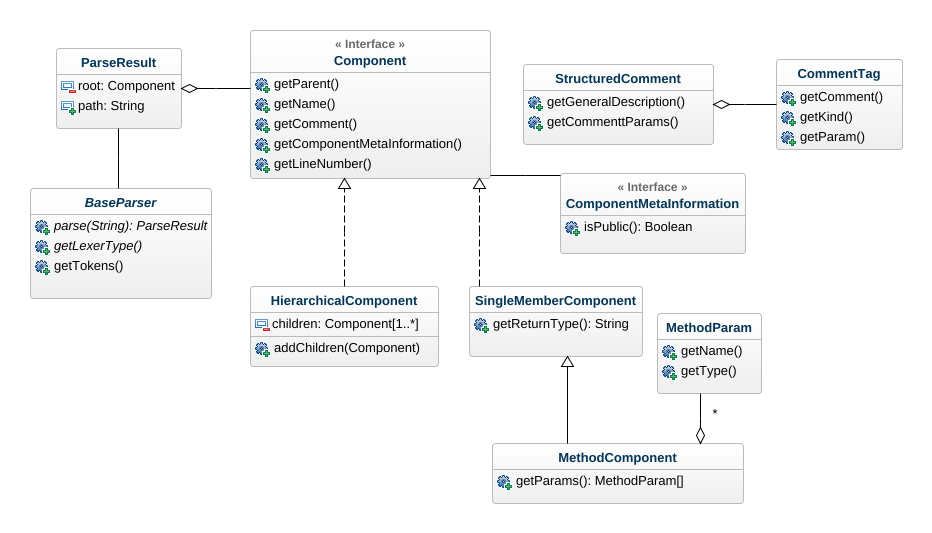
\includegraphics[height=9cm,keepaspectratio,angle=90]{figures/uml/parsing.png}
    \caption{UML-Diagramme aller Klassen, die relevant für das Parsen sind}
    \label{fig:uml_parsing}
\end{figure}
\chapter{UML-Diagramm: Metriken}\label{appendix_metrics_uml}
\begin{figure}[ht!]
\fontsize{5}{10}\selectfont
    \centering
    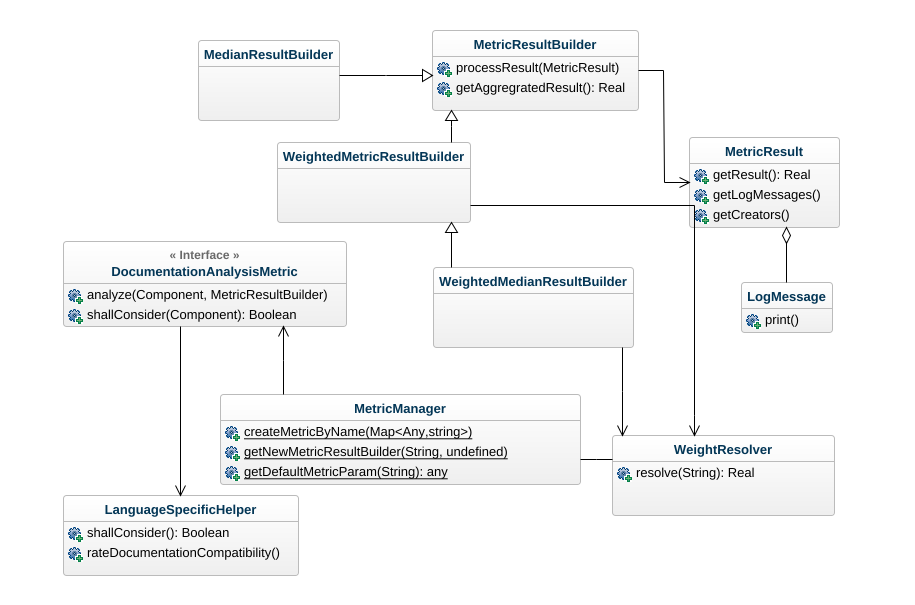
\includegraphics[height=10cm,keepaspectratio,angle=90]{figures/uml/metriken.png}
    \caption{UML-Diagramme aller Klassen, die relevant für die Metriken sind}
    \label{fig:uml_metrics}
\end{figure}
\chapter{Konfiguration des Tools}
\begin{description}
        \item[include]  Alle Dateien, die bei der Bewertung der Dokumentationsqualität berücksichtigt werden müssen
        \item[exclude]  Teilmenge von include, enthält Dateien, die nicht weiter betrachtet werden müssen
        \item[metrics]  Alle Metriken, die das Tool verwenden soll. Dies ist ein Array von Objekten mit der Struktur \enquote{(name,weight, unique\_name, params)}, wobei \textit{weight} das Gewicht der jeweiligen Metrik ist (Bei Algorithmen ohne Relevanz des Gewichts wird es ignoriert), \textit{name} der Name der Metrik und \textit{params} ein Objekt mit den Parametern der Metrik
        \item[absolute\_threshold] Mindestwert der Bewertung, die erreicht werden muss, sonst wird die Dokumentationsqualität nicht akzeptiert
       
          \item[builder] Der Algorithmus/\textit{ResultBuilder}, der die einzelnen Ergebnisse verarbeitet.
        
        \item[parser]  Kann verwendet, um die zu parsende Programmiersprache zu wählen. Dazu muss \textit{ParserFactory} angepasst werden
        
        \item[path\_weights] Ein Array von Objekten der Struktur \enquote{(path,weight)}. Wird verwendet, um einzelne Pfade höher oder niedriger zu gewichtet
        
         \item[component\_weights] Ein Array von Objekten der Struktur \enquote{(name,weight)}. Wird verwendet, um einzelne Komponenten höher oder niedriger zu gewichtet
         
         \item[default\_path\_weight] Das Standardgewicht für eine Datei, wenn keine passende Gewichtung gefunden wurde
         
         \item[default\_component\_weight] Das Standardgewicht einer Komponente, wenn keine passende Gewichtung gefunden wurde
         
         \item[state\_manager] Kann verwendet werden, um festzulegen, wie das letzte Ergebnis der Dokumentationsqualität gespeichert werden soll. Weitere Möglichkeiten können durch Erweiterung der \textit{StateManagerFactory} hinzugefügt werden.
         
         \item[relative\_threshold] Der maximale  relative Abstand zur letzten Dokumentationsqualität bevor eine Fehlermeldung geworfen wird.
         \item[builder\_params] Parameter für die \textit{MetricResultBuilder}. Diese wird aktuell nur von dem Squale-Builder (Kapitel \ref{chapter:squale}) genutzt
        
        
        
    \label{enum:tool_javadoc_conf}
\end{description}
\chapter{Implementierte Metriken}\label{appendix_metrics}

\begin{description}

\item[Anteil dokumentierter Komponenten an allen Komponenten]
\begin{description}
\item[]
    \item [Metrikname]  simple\_comment
    \item [Klassenname] SimpleCommentPresentMetric
    \item[Beschreibung] Berechnet den Anteil der dokumentierten Komponenten an allen Komponenten, kann Getter und Setter ignorieren
    \item[Quellen] \cite[S. 5]{HowDocumentationEvolvesoverTime}
\end{description}

\item[Anteil öffentlicher dokumentierter Komponenten]
\begin{description}
\item[]
    \item [Metrikname]  public\_members\_only
    \item [Klassenname] SimplePublicMembersOnlyMetric
    \item[Beschreibung] Berechnet den Anteil der öffentlichen dokumentierten Komponenten an allen öffentlichen Komponenten, kann Getter und Setter ignorieren
     \item[Quellen] \cite[S. 253]{JavadocViolationsandTheirEvolutioninOpen-SourceSoftware}
\end{description}

\item[Bestrafung langer undokumentierter Methoden]
\begin{description}
\item[]
    \item [Metrikname]  large\_method\_commented
    \item [Klassenname] SimpleLargeMethodCommentedMetric
    \item[Beschreibung] Bestraft undokumentierte Methoden je nach ihrer Länge
    \item[Quellen] Eigene Idee
\end{description}

\item[Vollständigkeit der Dokumentation von Methoden]
\begin{description}
\item[]
    \item [Metrikname]  method\_fully\_documented
    \item [Klassenname] SimpleMethodDocumentationMetric
    \item[Beschreibung] Prüft, ob alle Methodenparameter und Rückgabewert dokumentiert sind
    \item[Quellen] \cite[S. 5]{HowDocumentationEvolvesoverTime}
\end{description}
\clearpage
\item[Anteil dokumentierter Methoden unter
Berücksichtigung der LOC]
\begin{description}
\item[]
    \item [Metrikname]  commented\_lines
    \item [Klassenname] CommentedLinesRatioMetric
    \item[Beschreibung]  Berechnet den Anteil der \ac{LOC} der dokumentierten Methoden an allen \ac{LOC} aller Methoden
    \item[Quellen] Eigene Idee
\end{description}

\item[Flesch-Score]
\begin{description}
\item[]
    \item [Metrikname]  flesch
    \item [Klassenname] FleschMetric
    \item[Beschreibung]   Berechnet den Flesch-Score des Kommentars und bewertet so, ob der Kommentar verständlich ist
    \item[Quellen] \cite[S. 72]{AutomaticQualityAssessmentofSourceCodeComments:TheJavadocMiner}
\end{description}

\item[Kohärenz zwischen Kommentar und
Komponentenname]
\begin{description}
\item[]
    \item [Metrikname]  comment\_name\_coherence
    \item [Klassenname] CommentNameCoherenceMetric
    \item[Beschreibung]  Prüft, ob der Kommentar und der Name der dokumentierten Komponente sehr ähnlich sind oder keine Ähnlichkeit haben, arbeitet nur mit Methoden
    \item[Quellen] \cite[S. 86ff ]{Qualityanalysisofsourcecodecomments}
\end{description}

\item[Verwendung bestimmter Wörter bestrafen]
\begin{description}
\item[]
    \item [Metrikname]  certain\_terms
    \item [Klassenname] CertainTermCountMetric
    \item[Beschreibung]  Bestraft das Vorkommen bestimmter Wörter (wie z.~B. Abkürzungen)
     \item[Quellen] Inspiriert von Verbot lateinischer Ausdrücke nach \cite{HowtoWriteDocCommentsfortheJavadocTool}
\end{description}

\item[Bewertung der Formatierung]
\begin{description}
\item[]
    \item [Metrikname]  formatting\_good
    \item [Klassenname] FormattingGoodMetric
    \item[Beschreibung] Überprüft, ob korrekte Tags verwendet wurde, HTML-Tags geschlossen wurden und bei langen Methoden überhaupt eine Formatierung verwendet wurden
     \item[Quellen] Inspiriert von Regel in Checkstyle \cite{checkstyle_doc_metrics}
\end{description}

\clearpage
\item[Rechtschreibfehler bestrafen] 

\begin{description}
\item[]
    \item [Metrikname]  spellling
    \item [Klassenname] SpellingMetric
    \item[Beschreibung]Sucht nach Rechtschreibfehlern und bestraft sie
    \item[Quellen] Eigene Idee
\end{description}

\item[Erwähnung von Randfällen bei Methodenparameter
und -rückgabewerte]
\begin{description}
\item[]
    \item [Metrikname]  edge\_case
    \item [Klassenname] EdgeCaseMetric
    \item[Beschreibung] Prüft, ob bei der Dokumentation von Parametern die Behandlung des Wertes \textit{null} erwähnt wird
       \item[Quellen] Inspiriert von Idee in  \cite{javadoc_coding_standards}. In \cite[S.~1ff.]{@tComment:TestingJavadocCommentstoDetectComment-CodeInconsistencies} wird ebenfalls auf einer ähnlichen Art und Weise die Erwähnung von Randfällen geprüft, dort aber auch, ob diese Angaben korrekt sind
\end{description}


\item[Gunning-Fog-Index]
\begin{description}
\item[]
    \item [Metrikname]  gunning\_fog
    \item [Klassenname] GunningFogMetric
    \item[Beschreibung] Berechnet den Gunning-Fog-Index des Kommentars und bewertet so, ob der Kommentar verständlich ist
     \item[Quellen] \cite[S. 71]{AutomaticQualityAssessmentofSourceCodeComments:TheJavadocMiner}
\end{description}
 \end{description}

\chapter{Bilder des Tools}\label{chapter:pictures_tool}
In diesem Kapitel sind zwei Bilder des \textit{DoxEvaluators} abgedruckt, welche die zwei möglichen Ausgaben des Programms zeigen (Dokumentationsqualität ausreichend und nicht ausreichend):
\begin{figure}[htbp!]
    \centering
    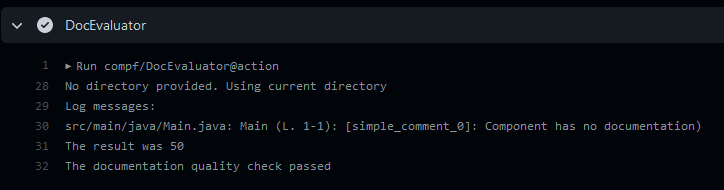
\includegraphics[width=\columnwidth]{figures/appendix/passed.png}
    \caption{Foto vom Tool: Dokumentationsqualität ausreichend}
    \label{fig:passed}
\end{figure}
\begin{figure}[htbp!]
    \centering
    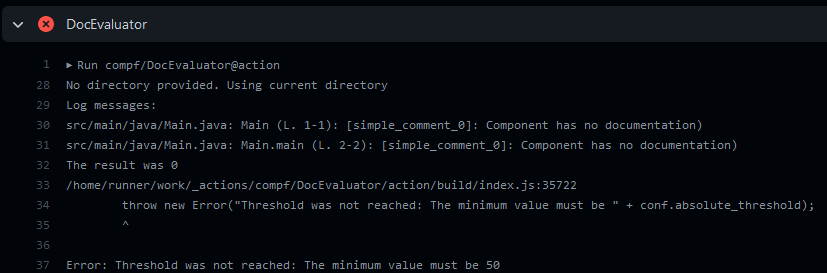
\includegraphics[width=\columnwidth]{figures/appendix/absolute_threshold.png}
    \caption{Foto vom Tool: Dokumentationsqualität zu schlecht}
    \label{fig:absolute}
\end{figure}

\end{appendices}
	


\clearpage
\chapter*{Erklärung zur selbstständigen Abfassung der Bachelorarbeit}

Ich versichere, dass ich die eingereichte Bachelorarbeit selbstständig und ohne unerlaubte Hilfe verfasst habe. Anderer als der von mir angegebenen Hilfsmittel und Schriften habe ich mich nicht bedient. Alle wörtlich oder sinngemäß den Schriften anderer Autoren entnommenen Stellen habe ich kenntlich gemacht. \\


\bigskip
\bigskip
\bigskip
\bigskip
\noindent
Osnabrück \today\\

\bigskip
\bigskip
\bigskip
\bigskip
\noindent
Timo Schoemaker
\end{document}




\begingroup
\renewcommand{\cleardoublepage}{} % TODO maybe removing this and next
\renewcommand{\clearpage}{}
\chapter{Evaluation}\label{chapter:eval}
\endgroup
	\newcommand{\checkpmd}{\textit{Checkstyle} und \textit{PMD} }
\newcommand{\doceval}{\textit{DocEvaluator} }
In diesem Kapitel soll das Programm evaluiert werden, um zu prüfen, ob der \doceval eine gute heuristische Aussage über den Stand der Dokumentationsqualität treffen kann und in der Praxis auch einsetzbar ist. Dazu wird der \textit{DocEvaluator} mit \textit{Checkstyle} und \textit{PMD} verglichen, indem drei exemplarische Open-Source-Projekte mit allen drei Programmen analysiert werden und die Treffergenauigkeit und Geschwindigkeit der Programme verglichen werden. Zunächst müssen diese drei Projekte ausgewählt werden, was in Kapitel \ref{chapter:choosing_project} erläutert wird. Anschließend wird in Kapitel \ref{chapter:quality} beschrieben, wie die Evaluation der Treffergenauigkeit durchgeführt wird. In Kapitel \ref{chapter:speed} wird die Geschwindigkeitsevaluation durchgeführt. Zum Abschluss der Evaluation werden die Ergebnisse der Evaluation in Kapitel \ref{chapter:eval_conclusion} resümiert. 

\clearpage

\section{Wahl der zu analysierenden Projekte}\label{chapter:choosing_project}
Zur Durchführung der Evaluation wurden verschiedene Softwareprojekte aus GitHub heruntergeladen. Grundsätzlich kann der Vergleich mit jedem Java-Projekt durchgeführt werden, dennoch wurden einige Bedingungen festgelegt, die bei der Auswahl der Projekte eine wichtige Rolle spielen. Diese Bedingungen werden in der folgenden Auflistung präsentiert:

\begin{enumerate}
    \item \label{enum:size} Die Projekte müssen mindestens einen Umfang von 10~000 \ac{LOC} haben
    \item \label{enum:already_cited} Die Projekte müssen bereits in einer in dieser Bachelorarbeit zitierten Quelle in puncto Dokumentationsqualität analysiert worden sein
    \item \label{enum:parsing_error}  Die Projekte sollen möglichst wenige Parsing-Fehler beim \doceval produzieren. Bei mehr als zwei Fehlern wird ein Projekt nicht betrachtet. Können jedoch Fehler folgenlos behoben werden, so kann das Projekt dennoch betrachtet werden
    \item Das größte Projekt sollte mindestens zehnmal so groß sein wie das kleinste Projekt
\end{enumerate}

Die \ac{LOC} sollen nur als sehr grobe Heuristik der Größe eines Softwareprojektes verstanden werden und enthalten nur den reinen Code ohne Kommentare. Dabei wird heuristisch vermutet, dass mit steigender \ac{LOC} die Anzahl der Komponenten in einem Softwareprojekt steigt, wobei all diese Komponenten fehlerhaft (oder gar nicht) dokumentiert sein können. Somit dienen die \ac{LOC} als approximative Schätzung der zu erwartenden Fehler. 

 Durch die Bedingung in Nr. \ref{enum:size} wird sichergestellt, dass eine ausreichende Anzahl an Fehlern in der Dokumentation zu erwarten ist, um eine gute Analyse der Dokumentationsqualität  und eine aussagekräftige Bewertung der Geschwindigkeit zu ermöglichen. Durch die Bedingung in Nr.  \ref{enum:already_cited} werden nur Projekte in Betracht gezogen, die bereits in der wissenschaftlichen Literatur berücksichtigt wurden und daher (zumindest für den jeweiligen Autor der Quelle) geeignet für eine Analyse der Dokumentation sind. Mit der Bedingung in Nr. \ref{enum:parsing_error} wird eine Verzerrung zugunsten oder zuungunsten des \textit{DocEvaluators} vermieden, denn durch Parsing-Fehler können Komponenten falsch analysiert werden, die von den anderen Tools richtig analysiert werden. Indirekt wird dadurch gefordert, dass ein Projekt keine neueren Java-Funktionen verwendet, da  der \textit{DocEvaluator} nur Java bis Version 8 unterstützt. Die letzte Bedingung ist besonders für die Bewertung der Geschwindigkeit relevant, da so geprüft werden kann, ob der \doceval auch bei größeren Projekten noch in annehmbarer Zeit ein Ergebnis berechnen kann. 
 
 \subsubsection{Analysierte Projekte}\label{chapter:eval_projects}
 Die folgende Auflistung zeigt die gewählten Projekte für die Evaluation. Die Quellen verweisen auf das Verzeichnis in GitHub, das von den drei Tools analysiert werden soll.  In runden Klammern dahinter befinden sich die  (auf Zehntausenderstelle gerundeten) \ac{LOC}. 
 \begin{itemize}
  \item Log4J Version 1 \cite{log4j} (20~000)
    \item ArgoUML \cite{argouml} (17~000) 
     \item Eclipse \ac{JDT} \cite{eclipsejdt} (400~000)
 \end{itemize}
 
 ArgoUML und Eclipse wurden in \cite[S.~74] {AutomaticQualityAssessmentofSourceCodeComments:TheJavadocMiner} bewertet, wobei hier nur Eclipse \ac{JDT} betrachtet werden soll, da das gesamte Eclipse-Projekt zu umfassend ist. Log4J wurde in \cite[S.~267] {@tComment:TestingJavadocCommentstoDetectComment-CodeInconsistencies} betrachtet. 

 Bei allen Projekten traten zunächst Parsing-Fehler auf. Dies lag allerdings in den meisten Fällen daran, dass auskommentierte Methoden noch ein Javadoc-Präfix hatten. Dies kann vom \doceval nicht korrekt verarbeitet werden. Da diese Methoden offensichtlich nicht verwendet werden und keinen Einfluss auf die Qualität der Dokumentation haben können, wurden sie ersatzlos entfernt. Bei einem Fehler in Eclipse \ac{JDT} konnte der \doceval eine Datei mit mehr als 3000 Codezeilen nicht verarbeiten. Diese Datei wurde bei der Evaluation von allen Programmen ignoriert.

\section{Analyse der Qualität}\label{chapter:quality}
Durch die Evaluation der Qualität soll geprüft werden, ob der \doceval trotz des in Kapitel \ref{chapter_conception}
 beschriebenen abstrakten Formates eine Java-Datei richtig parsen kann und alle für die Dokumentation relevanten Informationen korrekt extrahieren kann. Zur Durchführung der Evaluation muss zunächst definiert werden, welche Funktionen der einzelnen Programme miteinander verglichen werden können, da die Programme unterschiedliche Aspekte der Dokumentation überprüfen und die Darstellung der Ergebnisse im Vergleich zum \textit{DocEvaluator} abweicht.

\checkpmd können als fehlersuchend bezeichnet werden. Sie prüfen die einzelnen Komponenten eines Programms und finden Abweichungen von vorher definierten Regeln. Eine solche Regel kann beispielsweise sein, dass jede öffentliche Methode dokumentiert sein muss, dass bestimmte Wörter nicht verwendet werden dürfen oder dass die Syntax der Dokumentation gültig sein muss. Damit sind sie vergleichbar mit den Metriken aus den Kapiteln \ref{chapter:metrics_coverage}  und \ref{chapter:metrics_errors}, welche ebenfalls bestimmte Fehler suchen und bei einem Verstoß gegen die Regeln eine Warnmeldung ausgeben. Allerdings berechnen \checkpmd keine Metriken, sondern finden nur die besagten Verstöße gegen die definierten Regeln. Somit kann ein Entwickler sehen, dasś ein Projekt beispielsweise 100 Verstöße gegen die Dokumentationsrichtlinien hat, erfährt aber nicht, ob die Anzahl der Verstöße unter Berücksichtigung der Projektgröße schwerwiegend ist und erhält keine normierte Bewertung, die dem Entwickler bei der Beurteilung der Dokumentationsqualität hilft. 

Im Gegensatz dazu verwendet der \doceval Metriken, die stets einen Wert von 0 bis 100 zurückgeben, sodass ein Entwickler weiß, dass ein hoher Wert für eine hohe Qualität steht. Außerdem kann der \doceval auch die Semantik des Kommentars heuristisch prüfen, um zu erfahren, ob der Kommentar verständlich ist und nicht redundant ist (vgl. Kapitel \ref{chapter:metrics_semantic}). Nichtsdestotrotz gibt der \doceval auch Warnmeldungen aus, wenn er bestimmte Komponenten schlechter bewerten muss.

Aus diesen Gründen wird die Evaluation nicht mit den Metriken an sich, sondern mit den Warnmeldungen der jeweiligen Tools durchgeführt. Jedes Programm wird mit einem Verweis auf das zu analysierende Projekt aufgerufen und die Ausgaben der Programme werden in separaten Dateien umgeleitet.  Diese Dateien dienen dann als Grundlage für die spätere Evaluation. 

\subsubsection{Durchführung der Evaluation}
Wie im vorherigen Absatz beschrieben, dienen die Logdateien der drei Programme als Datengrundlage für die Evaluation. Jede Zeile in diesen Logdateien enthält mindestens den Dateipfad des gefundenen Fehlers, die Zeilennummer des Fehlers und einen Fehlercode als Zeichenkette.  Wenn die drei Programme einen übereinstimmenden Fehler finden, sollte es in allen drei Logdateien einen Eintrag geben, bei dem der Dateipfad identisch ist, die Zeilennummer innerhalb eines gewissen Intervalls identisch ist und die der Fehlercode identisch ist. Die Zeilennummer muss nicht zwingend identisch sein, da  \checkpmd die exakte Zeile des Fehlers ausgeben, während der \doceval nur ein Intervall ausgibt, in dem der Fehler liegt. Beispielsweise wird von \checkpmd bei einem unzulässigen Wort die exakte Zeile des Wortes genannt. Da die drei Tools unterschiedliche Fehlercodes ausgeben, werden diese so kategorisiert, dass Verstöße, welche von mehr als einem Tool erkannt werden, einen eigenen Fehlercode erhalten. Alle anderen Verstöße erhalten einen allgemeinen programmspezifischen Fehlercode, der somit keine näheren Informationen über die Art des Fehlers hergibt.

Basierend auf diesen Vorbereitungen kann nun für jeden Fehler jedes Programm gefunden werden, das diesen Fehler entdeckt hat. Beispielsweise kann ein Fehler von allen drei Programmen, nur von \textit{Checkstyle} oder ausschließlich von \textit{PMD} und \doceval gefunden werden. Mathematisch gesehen kann die Potenzmenge der Menge \textit{\{Checkstyle, PMD, DocEvaluator\}} genommen werden, wodurch alle möglichen Kombinationen an Programmen entstehen, die einen bestimmten Fehler erkennen können. Durch Zählen der Fehler pro Programmkombination lässt sich bewerten, welche Programme besonders viele Fehler finden, die andere Programme nicht erkennen und ob alle drei Programme viele gemeinsame Fehler finden. 


\subsubsection{Auswahl der Regeln}
Zum Vergleich der drei Programme müssen zunächst Regeln festgelegt werden, bei denen die Programme eine Warnmeldung ausgeben. Bei \checkpmd{} erfolgt die Konfiguration über  Extensible-Markup-Language-Dateien. Beim \doceval erfolgt die Konfiguration über das in Kapitel \ref{chapter:conf} beschriebene \ac{JSON}-Format. Bei der Auswahl der Regeln muss beachtet werden, dass \checkpmd auch andere Fehler wie z.~B. komplexe Methoden finden können. Diese sind in diesem Kontext nicht relevant und werden ignoriert. Außerdem können die drei Programme zum Teil unterschiedliche Fehler finden, da beispielsweise \textit{PMD} (anders als \textit{Checkstyle}) den Inhalt der Dokumentation auf das Auftauchen bestimmter Begriffe prüfen kann.  \textit{Checkstyle} kann aber dafür (anders als \textit{PMD}) prüfen, ob die Block-Tags in der richtigen Reihenfolge definiert werden. Die letztere Regel wird vom \doceval in der ausgelieferten Fassung nicht geprüft. Alle drei Programme können jedoch prüfen, ob eine Komponente dokumentiert ist oder nicht. Tabelle \ref{tab:inters_rules} vergleicht die Überschneidungen der Regeln, welche die drei Programme anwenden können. Dabei stehen (sowohl hier als auch im Rest des Kapitels 5) die Abkürzungen \textit{CS} für \textit{Checkstyle} und \textit{DE} für \textit{DocEvaluator}.

\begin{table}[]
    \centering
    \begin{tabular}{m{4.5cm}|m{4.5cm}|m{4.5cm}}
     \textbf{CS} $\cap$ \textbf{DE}  & \textbf{PMD} $\cap$ \textbf{DE} & \textbf{PMD} $\cap$ \textbf{DE} $\cap$  \textbf{CS}  \\\hline
     \begin{itemize}
        \item Komponente dokumentiert
        \item Methode vollständig dokumentiert
         \item Fehler in Javadoc
     \end{itemize}
      & 
      \begin{itemize}
          \item  Komponente dokumentiert

          \item Bestimmte Wörter in Kommentar verbieten
      \end{itemize}
      & 
       \begin{itemize}
          \item  Komponente dokumentiert
         
      \end{itemize}
      \\\hline
    \end{tabular}
    \caption{Überschneidungen der Regeln der drei Programme}
    \label{tab:inters_rules}
\end{table}

Aus der Tabelle lässt sich entnehmen, dass der \doceval mit \textit{Checkstyle} die meisten Übereinstimmungen hat. Beide Programme können die Vollständigkeit der Methodendokumentation und typische Fehler in Javadoc-Kommentaren (wie z.~B. fehlerhaftes HTML) finden. PMD und der \doceval können bestimmte Wörter in der Dokumentation bemängeln, die in einer Dokumentation vermieden werden sollten. Alle drei Programme können das Vorhandensein der Dokumentation überprüfen. Allerdings ignoriert \textit{PMD} alle privaten Komponenten außer Felder. Vor allem bei Checkstyle gibt es zudem viele Regeln, die von den anderen beiden Programmen nicht gefunden werden und auf der Webseite \cite{checkstyle_doc_metrics} aufgelistet werden.

Da ein Vergleich der drei Tools somit nur eingeschränkt möglich ist, wird sich die qualitative Evaluation nur auf den Kernbereich beschränken. Es werden also nur die Regeln verwendet, die von mindestens zwei Tools unterstützt werden. Dies sind alle Regeln in Tabelle \ref{tab:inters_rules}. Da somit nur relativ leichte Fehler gefunden werden, können die Ergebnisse der Evaluation dazu verwendet werden, um die Parsing-Qualität zu ermitteln, denn wenn solche grundlegenden Fehler (wie z.~B. das Nichtvorhandensein der Dokumentation) nicht gefunden werden, besteht eine erhebliche Chance, dass eine Java-Datei falsch interpretiert wird. 



\subsection{Ergebnisse}

Tabelle \ref{tab:eval_results} listet die Anzahl der gefundenen Fehler (gemäß Tabelle \ref{tab:inters_rules}) auf. In den Spalten werden die Fehler nach dem Projekt gruppiert. Die ersten drei Zeilen beschreiben, wie viele Fehler die einzelnen Tools pro Projekt gefunden haben. So hat  der \textit{DocEvaluator} 1710 Fehler in \textit{Log4J} gefunden.  In den übrigen Zeilen wird aufgeführt, welche Kombinationen der Tools wie viele Fehler gefunden haben. Die Zeile mit der ersten Spalte \enquote{\{PMD, DE\}} beschreibt beispielsweise, dass \textit{PMD} und der  \textit{DocEvaluator} (aber nicht \textit{Checkstyle}) 41 Fehler bei \textit{Log4J}, 264 Fehler bei \textit{ArgoUML} und 253 Fehler bei \textit{Eclipse \ac{JDT}} gefunden haben. 
\sisetup{group-minimum-digits=4,table-number-alignment =center,table-format=5.0}
\begin{table}[]
    \centering
\begin{tabular}{c|S|S|S}
          & {Log4J} & {ArgoUML} & {Eclipse \ac{JDT}} \\ \hline
|DE|            & 1710 & 10054  & 17380      \\ \hline
|CS|            & 1590 & 9961   & 17638      \\ \hline
|PMD|           & 1008 & 9051   & 12702      \\ \hline\hline
\{DE\}          & 108   & 124     & 555         \\ \hline
\{CS\}          & 26    & 285     & 273         \\ \hline
\{PMD\}         & 86    & 377     & 298         \\ \hline
\{PMD, DE\}     & 41    & 264     & 253         \\ \hline
\{CS, DE\}      & 683   & 1266    & 5214       \\ \hline
\{PMD, CS\}     & 3     & 10      & 793         \\ \hline
\{PMD, CS, DE\} & 878   & 8400   & 11358      \\ \hline
\end{tabular}
    \caption{Anzahl der gefundenen Fehler pro Projekt}
    \label{tab:eval_results}
\end{table}

Aus der Tabelle ist ersichtlich, dass stets über 50~\% aller Fehler von allen drei Tools gefunden werden. Bei \textit{Eclipse \ac{JDT}} und \textit{Log4J} werden mehr als ein Viertel der Fehler von der Kombination  \textit{DocEvaluator} und \textit{Checkstyle} gefunden. Beim Projekt \enquote{ArgoUML} liegt diese Quote bei weniger als 15~\%.  Weniger als 10~\% der Fehler werden nur von einem Tool erkannt. 

Die Überschneidungen der Fehler lassen sich auch mit Venn-Diagrammen darstellen.  Die Abbildungen \ref{fig:log4j_venn}, \ref{fig:argo_venn} und  \ref{fig:eclipse_venn} zeigen für jedes Projekt die Überschneidungen der gefundenen Fehler. Die Abbildung \ref{fig:legend_venn} ist die Legende dieser drei Abbildungen:


\begin{figure}[ht!]
\centering
   \begin{subfigure}[b]{0.4\textwidth}
    \centering
\includesvg[scale=0.7,width=\textwidth]{figures/chapter5/log4j.svg}
    \caption{Venn-Diagramm: Log4J}
    \label{fig:log4j_venn}
\end{subfigure}
\hfill
\begin{subfigure}[b]{0.4\textwidth}
    \centering
\includesvg[scale=0.7,width=\textwidth]{figures/chapter5/argo.svg}
    \caption{Venn-Diagramm: ArgoUML}
    \label{fig:argo_venn}
\end{subfigure}
\hspace{10cm}
\begin{subfigure}[b]{0.4\textwidth}
    \centering
\includesvg[scale=0.7,width=\textwidth]{figures/chapter5/eclipse.svg}
    \caption{Venn-Diagramm: Eclipse \ac{JDT}}
    \label{fig:eclipse_venn}
\end{subfigure}
\hspace{3.4cm}
\begin{subfigure}[b]{0.25\textwidth}
    \centering
\includesvg[width=1\textwidth]{figures/chapter5/legende_venn.svg}
\vspace{0.3cm}
    \caption{Legende der Venn-Diagramme}
    \label{fig:legend_venn}
\end{subfigure}
\end{figure}

  Auch hier zeigt der graue Bereich visuell, dass die drei verglichenen Tools viele Fehler gemeinsam finden.  Dies ist vor allem bei \textit{ArgoUML} deutlich, da der graue Kreis fast alle anderen Kreise großflächig überdeckt. Bei den anderen beiden Projekten ist zudem eine große Überschneidung von \textit{Checkstyle} und \doceval (hellbraun) zu erkennen. Bei \textit{Log4J} zeigt das Diagramm einen im Vergleich zu den anderen Projekten größeren Bereich (dunkelblau) an Fehlern, die nur von \textit{PMD} gefunden werden. Auch der Bereich der exklusiv vom \textit{DocEvaluator} gefundenen Fehler (rot) ist bei \textit{Log4J} größer. Die nur vom \textit{DocEvaluator} und \textit{PMD} gefundenen Fehler (lila) sind bei  \textit{Eclipse \ac{JDT}} nicht zu erkennen, bei den anderen Venn-Diagrammen allerdings schon. Dafür scheint es bei  \textit{Eclipse \ac{JDT}} relativ viele Fehler zu geben, die nur von \checkpmd gefunden werden, da der hellblaue Abschnitt nur dort sichtbar ist. Außerdem gibt es bei  \textit{Eclipse \ac{JDT}} mehr Fehler, die nur von \textit{Checkstyle} gefunden werden, da der grüne Bereich größer ist. 

Um die Trefferrate mathematisch auszudrücken, kann die Formel
\begin{equation}\label{eq1}
    1-\frac{\text{\{DE\}}}{|\text{DE}|}
\end{equation} verwendet werden. Diese gibt in Prozent an, wie viele Fehler, die vom \doceval gefunden werden, auch von den anderen beiden Tools gefunden werden. Demgegenüber kann auch ermittelt werden, wie viele Fehler von \textit{Checkstyle} oder \textit{PMD} gefunden wurden, die auch vom \doceval erkannt wurden:

\begin{equation}\label{eq2}
    1-\frac{\text{\{CS\}}+\text{\{PMD\}}+\text{\{CS,PMD\}}}{|\text{PMD}|+|\text{CS}|}
\end{equation}

Tabelle \ref{tab:hit_rate} zeigt basierend auf den genannten Formeln (\ref{eq1} und \ref{eq2}) die Treffergenauigkeit des \textit{DocEvaluators} für jedes analysierte Projekt:
\begin{table}[]
    \centering
    \begin{tabular}{c|c|c|c}
    Formel & Log4J & ArgoUML & Eclipse \ac{JDT} \\ \hline
    \ref{eq1} &   93,68~\% &	98,77~\% &	96,81~\% \\\hline
     \ref{eq2} & 95,57~\% &	96,47~\% &	95,50~\% \\\hline

    \end{tabular}
    \caption{Trefferrate des \textit{DocEvaluators} gemäß den Formeln \ref{eq1} und \ref{eq2}}
    \label{tab:hit_rate}
\end{table}
Es ist klar erkennbar, dass die Trefferrate unabhängig von der Formel und dem analysierten Projekt größer als 90~\% ist, sodass die meisten Fehler, die vom \doceval gefunden werden, von mindestens einem anderen Tool gefunden werden. Zudem werden die meisten Fehler, die von \textit{Checkstyle} oder \textit{PMD} gefunden werden, auch vom \doceval gefunden.






\subsection{Bewertung der Qualitätsevaluation}
Insgesamt zeigt die Evaluation der Qualität, dass der \doceval eine hohe Abdeckung mit \checkpmd hat und somit die meisten von diesen Tools gefundenen Fehler auch findet. Somit ist das abstrakte Format zur Repräsentation einer Quellcodedatei geeignet, um die meisten Aspekte, welche für die Dokumentation relevant sind, zu beschreiben. Allerdings wurde diese Evaluation auf größere Projekte (über 10~000 \ac{LOC}) beschränkt, sodass nicht geprüft wurde, ob der \doceval auch bei kleineren Projekten eine genaue Einschätzung der Dokumentationsqualität gibt. Tendenziell wird die Trefferrate kleiner sein, da durch die geringere Größe jeder nicht gefundene Fehler ein höheres Gewicht hat. 

Während der Evaluation wurde geprüft, warum einige Fehler nicht vom \doceval gefunden wurden. In einigen Fällen waren dies einfache Fehler, die bereits behoben sind, sodass dadurch die Trefferrate erhöht wurde. In anderen Fällen gibt es größere strukturelle Probleme, die nicht mehr leicht behebbar sind. Einige dieser Fehler werden im Folgenden präsentiert: 
\subsubsection{Fehler durch verschiedene Zeilennummerierung}

Einige Fehler sind keine Fehler des \textit{DocEvaluators} an sich, sondern sind in der Methodik der Evaluation begründet. Um gemeinsame Fehler zu finden, müssen die gefundene Fehler pro Tool abgeglichen werden, wozu die Zeilennummer elementar ist. Allerdings gibt es Unterschiede bei der Festlegung der Zeilennummer. Der \doceval verwendet in seiner Logausgabe ein Zeilennummerintervall, der mit der Zeile des Bezeichners der Komponente endet und dessen Anfang durch Subtraktion der Anzahl der Zeilen der Dokumentation von der Zeile des Bezeichners definiert wird. Die anderen Tools verwenden die exakte Zeile eines Fehlers. In den meisten Fällen ist dies kein Problem, da diese Zeilennummer von \checkpmd innerhalb des vom \doceval beschriebenen Intervalls liegen muss. Listing \ref{lst:multiline_method} zeigt ein Beispiel, wo es problematisch wird.

		\begin{figure}[ht!]
			\lstinputlisting
			[caption={Methode auf viele Zeilen verteilt},
			label={lst:multiline_method},
			captionpos=b,language=java, basicstyle=\footnotesize, tabsize=1, showstringspaces=false,  numbers=left]
			{figures/chapter5/multiline_method.java}
		\end{figure}
Besonders an dieser Methode ist, dass die Parameter auf verschiedenen Zeilen verteilt ist. Während \textit{Checkstyle} bei einem undokumentierten Parameter die exakte Zeile eines nicht dokumentierten Parameters ausgibt (z.~B. Z. 5), würde der \doceval die Zeilen 1 bis 4 ausgeben, da die Dokumentation bei Zeile 1 beginnt und der Bezeichner der Komponente in Zeile 4 definiert ist. Ähnlich problematisch ist es, wenn zwischen der Dokumentation und dem Bezeichner noch Annotationen stehen, sodass der Bezeichner um eine Zeile nach unten rutscht.  

\subsubsection{Klassen in Methoden}

In Java können Klassen in Methoden deklariert werden bzw. anonyme Klassen direkt instantiiert werden. Diese Klassen können ebenfalls Javadoc besitzen, werden allerdings vom \doceval ignoriert, da der \doceval jeglichen Code in Methoden nur unstrukturiert als Zeichenkette speichert und nicht weiterverarbeitet. Die anderen beiden Tools prüfen auch diese Klassen, sodass sie entsprechend einige Fehler finden, die der \doceval nicht mehr finden kann. 


\subsubsection{Fehler in einzeiligen Kommentaren bei PMD}
Anders als der \doceval und \textit{Checkstyle} berücksichtigt \textit{PMD} auch einzeilige Kommentare. Wenn ein einzeiliger Kommentar ein unzulässiges Wort enthält, so würde \textit{PMD} einen Fehler melden, aber der \doceval nicht, da er nur Javadoc-Kommentare prüft. Dadurch kommt es zu einer Verzerrung und der Anteil der alleinig von \textit{PMD} gefundenen Fehler wird überschätzt.  



 \section{Analyse der Geschwindigkeit} \label{chapter:speed}
 In diesem Abschnitt wird der \doceval mit \checkpmd bezüglich der Geschwindigkeit verglichen. Damit soll geprüft werden, ob das Tool nicht nur eine ausreichende Qualität besitzt, sondern auch in einer angemessenen Zeit ein Ergebnis liefert. Dies ist im \ac{CI/CD}-Kontext wichtig, da bei einer langen Laufzeit des Tools  die Bereitstellung eines geprüften Softwareprojektes verzögert wird und somit die Produktivität reduziert wird. 
 
 \subsubsection{Durchführung der Geschwindigkeitsevaluation}
 Zur Durchführung der Evaluation der Geschwindigkeit analysieren die drei Tools die in Kapitel \ref{chapter:eval_projects} genannten Projekte. Damit jedes Programm fair behandelt wird und eine ungefähr gleiche Menge an Analysen durchführen kann, werden die Regeln so beschränkt, dass nur noch das Vorhandensein von Dokumentation geprüft wird. So wird verhindert, dass beispielsweise der \textit{DocEvaluator} und \textit{Checkstyle} die Dokumentation von Methodenparameter überprüfen, während \textit{PMD} dies ignoriert. Bei jeder Analyse wird die Zeit gemessen, die vom Start eines Tools bis zu dessen Beendigung vergehen. 
 
 Die Ausgabe jedes Tools wird auf \enquote{dev/null} umgeleitet, sodass jegliche Ausgabe ignoriert wird. Dadurch können Schwankungen unberücksichtigt bleiben, die bei der Verwendung von Eingabe- und Ausgabegeräten auftreten. So sind die Ergebnisse näher an der tatsächlichen Verarbeitungsgeschwindigkeit.  Nachteilhaft an diesem Vorgehen ist, dass die Tools im Praxiseinsatz eine Ausgabe produzieren müssen, um überhaupt dem Entwickler helfen zu können, sodass dieser wichtige Aspekt hier ignoriert wird. 
 
 Die Analyse jedes Projektes mit jedem Tool wird zehnmal durchgeführt, um Schwankungen durch Hintergrundprozesse oder andere Einflussfaktoren auszugleichen. Die Evaluation der Geschwindigkeit wird auf einem Laptop mit dem Prozessor \enquote{i7-1165G7} mit 16 GB Arbeitsspeicher durchgeführt. Dabei wurden alle Programme auf dem Computer geschlossen und die Berechnungen wurden ohne grafische Benutzeroberfläche durchgeführt, um Schwankungen in der Laufzeit zu minimieren.  
 \subsection{Ergebnisse}\label{chapter:eval_speed_result}
 Die Tabellen \ref{tab:median_speed} und \ref{tab:std_speed} zeigen den Median und die Standardabweichung der benötigten Durchlaufzeit pro Tool und Projekt in Sekunden. Die Abbildungen \ref{fig:log4j_box}, \ref{fig:argo_box} und \ref{fig:eclipse_box} visualisieren den Inhalt der Tabellen als Boxplot. 
 
Im Verzeichnis \enquote{speed\_eval} des digitalen Anhangs befinden sich die Rohdaten der Geschwindigkeitsmessung, gruppiert nach dem analysierten Projekt. Auch die Originaldateien der Boxplots befinden sich dort. 
 \sisetup{group-minimum-digits=4,table-number-alignment =center,table-format=2.3,output-decimal-marker = {,}}
 \begin{table}[ht!]
     \centering
     \begin{tabular}{c|S|S|S}
        & {DE} & {CS} & {PMD}  \\\hline
        Log4J & 2.538 & 2.30 & 1.907\\\hline 
        ArgoUML & 16.965 & 9.301 & 7.917 \\\hline
        Eclipse \ac{JDT} & 69.148 & 27.316 & 21.586
     \end{tabular}
     \caption{Median der Laufzeit in Sekunden}
     \label{tab:median_speed}
 \end{table}
 
  \begin{table}[ht!]
     \centering
     \begin{tabular}{c|S|S|S}
        & {DE} & {CS} & {PMD}  \\\hline
        Log4J & 0,077 &  0,174 &  0,068\\\hline 
        ArgoUML & 0,197 &  0,083 & 0,157 \\\hline
        Eclipse \ac{JDT} & 1,594 & 0,265 & 0,270\\\hline
     \end{tabular}
     \caption{Standardabweichung der Laufzeit in Sekunden}
     \label{tab:std_speed}
 \end{table}
 
 \begin{figure}
 \centering
    \begin{subfigure}[b]{0.49\textwidth}
    \centering
\includesvg[width=\textwidth]{figures/chapter5/log4j_speed_boxplot.svg}
    \caption{Boxplot: Log4J}
    \label{fig:log4j_box}
\end{subfigure}
\hspace{0.01cm}
 \begin{subfigure}[b]{0.49\textwidth}
    \centering
\includesvg[width=\textwidth]{figures/chapter5/argo_speed_boxplot.svg}
    \caption{Boxplot: ArgoUML}
    \label{fig:argo_box}
\end{subfigure}

 \begin{subfigure}[b]{0.49\textwidth}
    \centering
\includesvg[,width=\textwidth]{figures/chapter5/eclipse_speed_boxplot.svg}
    \caption{Boxplot: Eclipse \ac{JDT} }
    \label{fig:eclipse_box}
\end{subfigure}
   
 \end{figure}
 

Aus den Tabellen und Boxplot-Diagrammen wird ersichtlich, dass der \doceval im Durchschnitt länger benötigt, um die Projekte zu bewerten. Wie aus dem Boxplot-Diagramm \ref{fig:log4j_box} zu entnehmen ist, gab es nur bei Log4J einen Ausreißer, bei dem \textit{Checkstyle} mehr Zeit benötigt hat.   Ansonsten war \textit{Checkstyle} stets schneller als der \textit{DocEvaluator}. \textit{PMD} analysiert am schnellsten ein Projekt. Der Unterschied in der Laufzeit zwischen dem \doceval und den anderen Tools steigt stark  mit wachsender Größe des analysierten Projektes.  Bei dem kleinsten Projekt \textit{Log4J} benötigt der \doceval  durchschnittlich die 1,103-fache Zeit im Vergleich zu \textit{Checkstyle}. Bei dem größten Projekt \textit{Eclipse \ac{JDT}} benötigt der \doceval durchschnittlich 2,53-mal so viel Zeit wie \textit{Checkstyle}. Beim \doceval und \textit{PMD} steigt die Standardabweichung mit der Größe des Projektes, während dieser Trend bei \textit{Checkstyle} nicht so eindeutig ist.

Bei dem Boxplot-Diagramm \ref{fig:log4j_box} zu \textit{Log4J} ist auch erkennbar, dass Ausreißer der Laufzeit nach oben häufiger sind als nach unten, da der Median sich stets im unteren Bereich des Boxplot-Quartils befindet. Bei den anderen Projekten ist dies aufgrund des größeren Zeitabstandes  zwischen dem \doceval und den anderen Tools  und der daraus resultierenden Verkleinerung der einzelnen Boxplots  nicht so klar im Boxplot ersichtlich, allerdings stimmt diese Aussage größtenteils auch dort. Nur bei der Analyse von \textit{ArgoUML} durch den \doceval (Abbildung \ref{fig:argo_box}) scheinen Abweichungen nach unten häufiger zu sein.

\subsection{Bewertung der Ergebnisse}
Insgesamt zeigt die Evaluation der Geschwindigkeit, dass der \doceval langsamer arbeitet als die anderen Programmen. Allerdings  bleibt die Laufzeit auf einem angemessenen Niveau, da die Verarbeitung von dem größten Projekt \textit{Eclipse \ac{JDT}} mit 400~000 \ac{LOC} im Durchschnitt nur etwas mehr als einer Minute benötigt. Nichtsdestotrotz ignoriert diese Analyse, dass die Ausgabe von Ergebnissen über die Konsole hier nicht berücksichtigt wurde und nur eine einfache Metrik angewendet wurde. Bei einem Experiment mit aktivierter Ausgabe wurden ähnliche Ergebnisse produziert, insbesondere ist der \doceval weiterhin das langsamste Programm. 

Für die schlechtere Laufzeit des \doceval im Vergleich zu \checkpmd lassen sich zwei Hauptargumente finden. So soll \textit{Node.Js}, welches die Plattform des Tools ist, langsamer sein als Java, in dem \checkpmd programmiert sind \cite{node_java_speed}.  Außerdem ist zu beachten, dass der \doceval Metriken berechnen soll und daher die Zwischenergebnisse aller Komponenten speichern muss, um daraus ein Gesamtergebnis mittels eines arithmetischen Mittelwerts oder eines anderen Algorithmus' berechnen zu können. Auch wenn dieses Gesamtergebnis bei der Laufzeitevaluation uninteressant ist, wird es dennoch berechnet, was zusätzliche Laufzeit benötigt. Dies erklärt auch die starke Steigerung des Zeitaufwands bei größeren Projekten.

\section{Fazit der Evaluation}\label{chapter:eval_conclusion}

Insgesamt zeigt die Evaluation sowohl bezüglich der Qualität als auch der Geschwindigkeit, dass der \doceval mit den anderen Tools mithalten kann. Zwar wird nicht jeder Fehler gefunden, aber die Trefferrate ist hoch und durch die Verwendung eines abstrakten Formates, das für mehrere Programmiersprachen geeignet ist, sind solche Abstriche nicht vermeidbar. 

Auch bei der Geschwindigkeit zeigt sich, dass der \doceval zwar im Extremfall zweieinhalbmal langsamer ist als die anderen Tools, allerdings ist die Laufzeit mit knapp 70 Sekunden im Extremfall bei einem großen Projekt noch in einem (relativ) angemessenen Rahmen. Nichtsdestotrotz ist es eine Überlegung wert, den \doceval weiter zu optimieren, damit die Laufzeit verbessert wird. 
\begingroup
\renewcommand{\cleardoublepage}{} % TODO maybe removing this and next
\renewcommand{\clearpage}{}
\chapter{Conclusion}\label{chapter:conclusion}
\endgroup
\label{sec:conclusion}
Ziel dieser Bachelorarbeit war es, ein Tool zu Bewertung der Dokumentation zu entwickeln, das in einem \ac{CI/CD}-Prozess eingebunden werden kann und nicht auf einer Programmiersprache beschränkt ist. Dabei beschränkt sich diese Bachelorarbeit auf strukturierte Kommentaren wie z.~B. Javadoc. Dieses Ziel wurde im Großen und Ganzen erreicht.

Durch die allgemein gehaltene Klassenstruktur für das Parsing ist es möglich, Quellcode in anderen Programmiersprachen bewerten zu lassen. Allerdings muss dafür ein entsprechender Parser geschrieben werden, welcher den Quellcode in die vorgegebene Struktur transformiert. Dabei ist es natürlich nicht möglich, jedes Detail abzubilden, sondern es müssen Abstriche gemacht werden. Nichtsdestotrotz können auch sprachspezifische Eigenheiten berücksichtigt werden, indem eine entsprechende abgeleitete Klasse von \textit{ComponentMetaInformation} gebildet wird und diese sprachspezifischen Informationen dort gespeichert werden. Diese Daten können von einem geeigneten \textit{LanguageSpecificHelper} dazu verwendet werden, um sprachabhängige Details bei der Bewertung der Dokumentation zu berücksichtigen. 

Auch das Parsen der strukturierten Kommentare erfolgt recht abstrakt, indem  die Informationen in den Beschreibungstexten unstrukturiert als Zeichenketten gespeichert werden, sodass die einzelnen Metriken diese Informationen weiterverarbeiten müssen. Da es Metriken gibt, die mit den einzelnen Wörtern ein eines Kommentars arbeiten und auch Metriken, welche die interne Struktur des Kommentars analysieren, wäre es ein mögliches Forschungsthema, wie diese zwei Darstellungen besser repräsentiert werden können. 

Um das Tool konfigurierbar zu halten, wurde ein Konzept für eine Konfigurationsdatei im \ac{JSON}-Format vorgestellt, das alle wichtigen Informationen enthält. Die Konfiguration kann auch über GitHub Actions durchgeführt werden, indem passende Umgebungsvariablen gesetzt werden.  So kann das Tool sowohl als reguläres Programm auf einem lokalen System verwendet werden als auch mittels GitHub Actions in den \ac{CI/CD}-Prozess eingebunden werden. Durch die flexible Konfiguration kann ein Nutzer frei entscheiden, welche Metriken er für sinnvoll hält und wie er sie gewichten will. Dabei überschreibt die Konfiguration mittels GitHub Actions stets die Konfiguration in der \ac{JSON}-Datei. Außerdem können die Metriken selbst begrenzt konfiguriert werden. Eine Nutzung des Tools auf anderen \ac{CI/CD}-Plattformen, die mit GitHub Actions vergleichbar sind,  ist prinzipiell ebenfalls möglich, da die Konfiguration von dem  übrigen Programm entkoppelt ist.

Für das Tool wurden bereits einige Metriken entwickelt, welche verschiedene Bereiche der Dokumentation analysieren können. Leider war eine Evaluation der einzelnen Metriken nicht möglich, sodass weiterhin offenbleibt, welche Metriken in welchen Situationen valide Ergebnisse liefern und wie eine sinnvolle Gewichtung der Metriken aussehen kann.  Weitere Metriken lassen sich durch Einfügen einer neuen abgeleiteten Klasse von \textit{DocumentationAnalysisMetric} bilden. Schwierig kann im konkreten Einzelfall allerdings das Finden einer geeigneten Funktion werden, welche die Werte der Metrik in das vorgegebene Intervall von 0 bis 100 transformiert. Mögliche Ideen für weitere Metriken lassen sich in \cite{checkstyle_doc_metrics} finden. Auch die wissenschaftliche Literatur liefert weitere Metriken, die fortschrittliche Techniken im Bereich des \ac{NLP} nutzen und daher im Rahmen dieser Bachelorarbeit zu komplex waren. Beispielhaft sei hier das Tool \enquote{iComment} aus  \cite[S.~145ff.]{icomment} genannt, bei dem geprüft wurde, ob die Dokumentation mit dem Code auch konsistent ist und somit korrekt und aktuell ist. Diese Metriken können als Inspiration genommen werden, um die Dokumentationsqualität umfassender analysieren zu können, sodass Entwickler bei der Identifikation und Behebung von mangelhafter Softwaredokumentation  besser unterstützt werden.





%Prints references
\printbibliography[title=Literature]


\clearpage 

%Appendix (comes after bibliography)

\renewcommand\appendixpagename{Anhänge}
\begin{appendices}


\chapter{Änderungen an der Parserdatei}\label{chapter:appendix_parser_changes}

\begin{table}[h!]
    \centering
    \begin{tabular}{m{0.75cm}|m{4cm}|m{10cm}}
        \textbf{Zeile} & \textbf{Änderung} & \textbf{Begründung} \\
         \hline
        116 & Deklaration Kommentar & Hier wird ein mehrzeiliger Kommentar definiert, dies ist hier ein Alias für den Token \textit{JCOMMENT}\\
        \hline
        127--128 & \textit{comment} als mögliches Präfix in Klassenmember & Hier wird dem Parser mitgeteilt, dass ein Bestandteil einer Klasse wie z. B. eine Methode einen Javadoc-Kommentar besitzen kann\\
        \hline
        47 & \textit{comment} als mögliches Präfix vor Datentyp & Hier wird dem Parser mitgeteilt, dass ein Datentyp (Klasse, Schnittstelle etc. ) einen Javadoc-Kommentar haben kann \\
        \hline
        404 & Zulassung von Javadoc in Methoden & Da Javadoc-Kommentare an beliebigen Stellen auftauchen können, auch wenn es nicht empfohlen wird und keinen Mehrwert bietet, wird hier sichergestellt, dass solche Kommentare nicht zu Warnungen oder Fehler von ANTLR4 führen. Diese Javadoc-Kommentare werden nichtsdestotrotz später ignoriert\\
        \hline
        34, 38& Zulassung von Kommentaren vor Paketdeklarationen und Imports & Hier werden Kommentare auch vor Paketdeklarationen und Import-Statements erlaubt, was vor allem bei Klassen mit Urheberrechtsangabe sinnvoll ist\\
        \hline
        105 & Zulassung von Kommentaren bei Enumerationen & Zwar werden Javadoc-Kommentare in Enumerationen mit diesem Tool nicht betrachtet, sie führen aber dennoch zu Warnungen und Fehlermeldungen. Daher werden sie hier zugelassen, aber später ignoriert \\
        \hline
        82, 83 & Erzeugung eines separaten Knotens für \textit{Extends}- und \textit{Implements}-Deklarationen & In der originalen Version der Parserdatei wurde die Definition der Basisklasse bzw. der implementierten Schnittstellen direkt über die Tokens \textit{EXTENDS} bzw. \textit{IMPLEMENTS} gelöst. Dies wurde in einem neuen Knoten \textit{extendClass} bzw. \textit{implementInterfaces} ausgegliedert, um so das Parsing etwas zu vereinfachen  \\
         
    \end{tabular}
    \caption{Änderungen an der Parserdatei}
    \label{tab:parser_changes}
\end{table}

\chapter{UML-Diagramm: Parser}\label{appendix_parsing_uml}
\begin{figure}[ht!]
\fontsize{5}{10}\selectfont
    \centering
    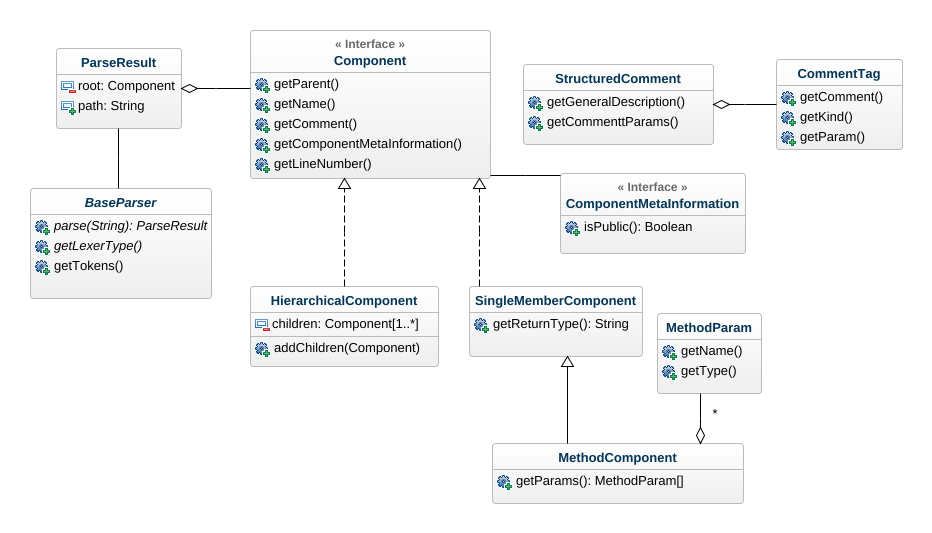
\includegraphics[height=9cm,keepaspectratio,angle=90]{figures/uml/parsing.png}
    \caption{UML-Diagramme aller Klassen, die relevant für das Parsen sind}
    \label{fig:uml_parsing}
\end{figure}
\chapter{UML-Diagramm: Metriken}\label{appendix_metrics_uml}
\begin{figure}[ht!]
\fontsize{5}{10}\selectfont
    \centering
    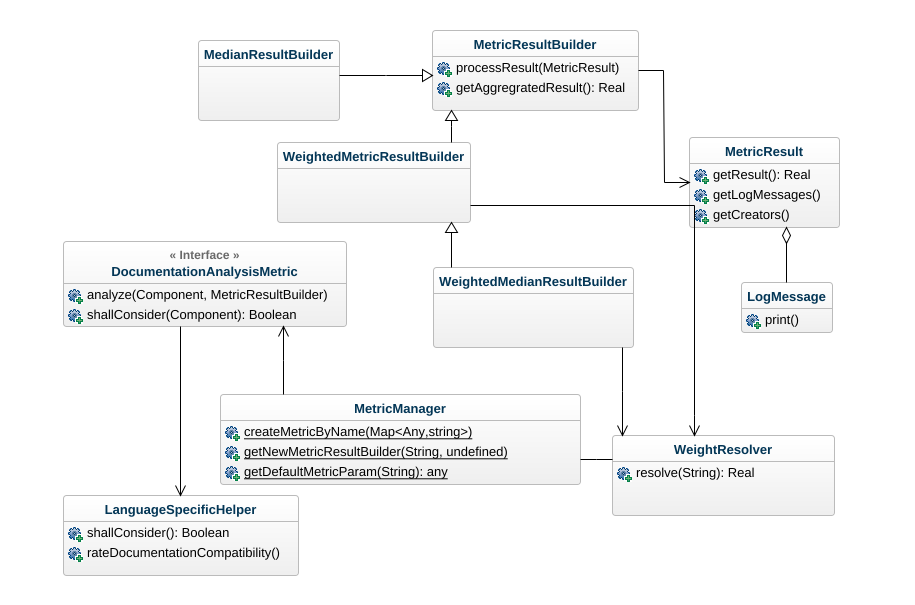
\includegraphics[height=10cm,keepaspectratio,angle=90]{figures/uml/metriken.png}
    \caption{UML-Diagramme aller Klassen, die relevant für die Metriken sind}
    \label{fig:uml_metrics}
\end{figure}
\chapter{Konfiguration des Tools}
\begin{description}
        \item[include]  Alle Dateien, die bei der Bewertung der Dokumentationsqualität berücksichtigt werden müssen
        \item[exclude]  Teilmenge von include, enthält Dateien, die nicht weiter betrachtet werden müssen
        \item[metrics]  Alle Metriken, die das Tool verwenden soll. Dies ist ein Array von Objekten mit der Struktur \enquote{(name,weight, unique\_name, params)}, wobei \textit{weight} das Gewicht der jeweiligen Metrik ist (Bei Algorithmen ohne Relevanz des Gewichts wird es ignoriert), \textit{name} der Name der Metrik und \textit{params} ein Objekt mit den Parametern der Metrik
        \item[absolute\_threshold] Mindestwert der Bewertung, die erreicht werden muss, sonst wird die Dokumentationsqualität nicht akzeptiert
       
          \item[builder] Der Algorithmus/\textit{ResultBuilder}, der die einzelnen Ergebnisse verarbeitet.
        
        \item[parser]  Kann verwendet, um die zu parsende Programmiersprache zu wählen. Dazu muss \textit{ParserFactory} angepasst werden
        
        \item[path\_weights] Ein Array von Objekten der Struktur \enquote{(path,weight)}. Wird verwendet, um einzelne Pfade höher oder niedriger zu gewichtet
        
         \item[component\_weights] Ein Array von Objekten der Struktur \enquote{(name,weight)}. Wird verwendet, um einzelne Komponenten höher oder niedriger zu gewichtet
         
         \item[default\_path\_weight] Das Standardgewicht für eine Datei, wenn keine passende Gewichtung gefunden wurde
         
         \item[default\_component\_weight] Das Standardgewicht einer Komponente, wenn keine passende Gewichtung gefunden wurde
         
         \item[state\_manager] Kann verwendet werden, um festzulegen, wie das letzte Ergebnis der Dokumentationsqualität gespeichert werden soll. Weitere Möglichkeiten können durch Erweiterung der \textit{StateManagerFactory} hinzugefügt werden.
         
         \item[relative\_threshold] Der maximale  relative Abstand zur letzten Dokumentationsqualität bevor eine Fehlermeldung geworfen wird.
         \item[builder\_params] Parameter für die \textit{MetricResultBuilder}. Diese wird aktuell nur von dem Squale-Builder (Kapitel \ref{chapter:squale}) genutzt
        
        
        
    \label{enum:tool_javadoc_conf}
\end{description}
\chapter{Implementierte Metriken}\label{appendix_metrics}

\begin{description}

\item[Anteil dokumentierter Komponenten an allen Komponenten]
\begin{description}
\item[]
    \item [Metrikname]  simple\_comment
    \item [Klassenname] SimpleCommentPresentMetric
    \item[Beschreibung] Berechnet den Anteil der dokumentierten Komponenten an allen Komponenten, kann Getter und Setter ignorieren
    \item[Quellen] \cite[S. 5]{HowDocumentationEvolvesoverTime}
\end{description}

\item[Anteil öffentlicher dokumentierter Komponenten]
\begin{description}
\item[]
    \item [Metrikname]  public\_members\_only
    \item [Klassenname] SimplePublicMembersOnlyMetric
    \item[Beschreibung] Berechnet den Anteil der öffentlichen dokumentierten Komponenten an allen öffentlichen Komponenten, kann Getter und Setter ignorieren
     \item[Quellen] \cite[S. 253]{JavadocViolationsandTheirEvolutioninOpen-SourceSoftware}
\end{description}

\item[Bestrafung langer undokumentierter Methoden]
\begin{description}
\item[]
    \item [Metrikname]  large\_method\_commented
    \item [Klassenname] SimpleLargeMethodCommentedMetric
    \item[Beschreibung] Bestraft undokumentierte Methoden je nach ihrer Länge
    \item[Quellen] Eigene Idee
\end{description}

\item[Vollständigkeit der Dokumentation von Methoden]
\begin{description}
\item[]
    \item [Metrikname]  method\_fully\_documented
    \item [Klassenname] SimpleMethodDocumentationMetric
    \item[Beschreibung] Prüft, ob alle Methodenparameter und Rückgabewert dokumentiert sind
    \item[Quellen] \cite[S. 5]{HowDocumentationEvolvesoverTime}
\end{description}
\clearpage
\item[Anteil dokumentierter Methoden unter
Berücksichtigung der LOC]
\begin{description}
\item[]
    \item [Metrikname]  commented\_lines
    \item [Klassenname] CommentedLinesRatioMetric
    \item[Beschreibung]  Berechnet den Anteil der \ac{LOC} der dokumentierten Methoden an allen \ac{LOC} aller Methoden
    \item[Quellen] Eigene Idee
\end{description}

\item[Flesch-Score]
\begin{description}
\item[]
    \item [Metrikname]  flesch
    \item [Klassenname] FleschMetric
    \item[Beschreibung]   Berechnet den Flesch-Score des Kommentars und bewertet so, ob der Kommentar verständlich ist
    \item[Quellen] \cite[S. 72]{AutomaticQualityAssessmentofSourceCodeComments:TheJavadocMiner}
\end{description}

\item[Kohärenz zwischen Kommentar und
Komponentenname]
\begin{description}
\item[]
    \item [Metrikname]  comment\_name\_coherence
    \item [Klassenname] CommentNameCoherenceMetric
    \item[Beschreibung]  Prüft, ob der Kommentar und der Name der dokumentierten Komponente sehr ähnlich sind oder keine Ähnlichkeit haben, arbeitet nur mit Methoden
    \item[Quellen] \cite[S. 86ff ]{Qualityanalysisofsourcecodecomments}
\end{description}

\item[Verwendung bestimmter Wörter bestrafen]
\begin{description}
\item[]
    \item [Metrikname]  certain\_terms
    \item [Klassenname] CertainTermCountMetric
    \item[Beschreibung]  Bestraft das Vorkommen bestimmter Wörter (wie z.~B. Abkürzungen)
     \item[Quellen] Inspiriert von Verbot lateinischer Ausdrücke nach \cite{HowtoWriteDocCommentsfortheJavadocTool}
\end{description}

\item[Bewertung der Formatierung]
\begin{description}
\item[]
    \item [Metrikname]  formatting\_good
    \item [Klassenname] FormattingGoodMetric
    \item[Beschreibung] Überprüft, ob korrekte Tags verwendet wurde, HTML-Tags geschlossen wurden und bei langen Methoden überhaupt eine Formatierung verwendet wurden
     \item[Quellen] Inspiriert von Regel in Checkstyle \cite{checkstyle_doc_metrics}
\end{description}

\clearpage
\item[Rechtschreibfehler bestrafen] 

\begin{description}
\item[]
    \item [Metrikname]  spellling
    \item [Klassenname] SpellingMetric
    \item[Beschreibung]Sucht nach Rechtschreibfehlern und bestraft sie
    \item[Quellen] Eigene Idee
\end{description}

\item[Erwähnung von Randfällen bei Methodenparameter
und -rückgabewerte]
\begin{description}
\item[]
    \item [Metrikname]  edge\_case
    \item [Klassenname] EdgeCaseMetric
    \item[Beschreibung] Prüft, ob bei der Dokumentation von Parametern die Behandlung des Wertes \textit{null} erwähnt wird
       \item[Quellen] Inspiriert von Idee in  \cite{javadoc_coding_standards}. In \cite[S.~1ff.]{@tComment:TestingJavadocCommentstoDetectComment-CodeInconsistencies} wird ebenfalls auf einer ähnlichen Art und Weise die Erwähnung von Randfällen geprüft, dort aber auch, ob diese Angaben korrekt sind
\end{description}


\item[Gunning-Fog-Index]
\begin{description}
\item[]
    \item [Metrikname]  gunning\_fog
    \item [Klassenname] GunningFogMetric
    \item[Beschreibung] Berechnet den Gunning-Fog-Index des Kommentars und bewertet so, ob der Kommentar verständlich ist
     \item[Quellen] \cite[S. 71]{AutomaticQualityAssessmentofSourceCodeComments:TheJavadocMiner}
\end{description}
 \end{description}

\chapter{Bilder des Tools}\label{chapter:pictures_tool}
In diesem Kapitel sind zwei Bilder des \textit{DoxEvaluators} abgedruckt, welche die zwei möglichen Ausgaben des Programms zeigen (Dokumentationsqualität ausreichend und nicht ausreichend):
\begin{figure}[htbp!]
    \centering
    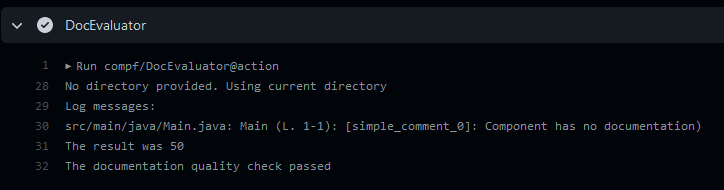
\includegraphics[width=\columnwidth]{figures/appendix/passed.png}
    \caption{Foto vom Tool: Dokumentationsqualität ausreichend}
    \label{fig:passed}
\end{figure}
\begin{figure}[htbp!]
    \centering
    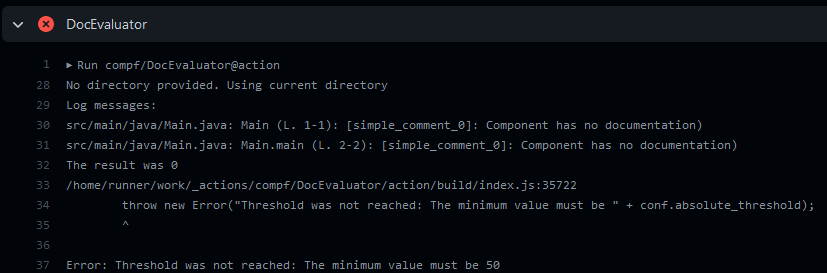
\includegraphics[width=\columnwidth]{figures/appendix/absolute_threshold.png}
    \caption{Foto vom Tool: Dokumentationsqualität zu schlecht}
    \label{fig:absolute}
\end{figure}

\end{appendices}
	



\chapter*{Erklärung zur selbstständigen Abfassung der Bachelorarbeit}

Ich versichere, dass ich die eingereichte Bachelorarbeit selbstständig und ohne unerlaubte Hilfe verfasst habe. Anderer als der von mir angegebenen Hilfsmittel und Schriften habe ich mich nicht bedient. Alle wörtlich oder sinngemäß den Schriften anderer Autoren entnommenen Stellen habe ich kenntlich gemacht. \\


\bigskip
\bigskip
\bigskip
\bigskip
\noindent
Osnabrück \today\\

\bigskip
\bigskip
\bigskip
\bigskip
\noindent
Timo Schoemaker
\end{document}

